\documentclass{book}

\usepackage[a4paper, total={6in, 8in}]{geometry}

% Failed attempt at setting wider margins for figures
\usepackage[export]{adjustbox}
\usepackage[french,english]{babel}
\usepackage{xspace}

\usepackage{amsmath}
\usepackage{amssymb}
\usepackage{amsfonts}
\usepackage{stmaryrd}

\usepackage{multicol}
\usepackage{float}

\input{include/bibliography}
\newcommand{\chapterdirectory}{.}
\newcommand{\definechapterdirectory}[1]{\def \chapterdirectory {#1}}

\usepackage{listings}
\lstset
{
   basicstyle=\footnotesize,
   numbers=left,
   stepnumber=1
}

\usepackage{caption}
\usepackage{subcaption}

\newtheorem{definition}{Definition}
\newtheorem{property}{Property}
\newtheorem{proposition}{Proposition}
\newtheorem{example}{Example}
\newtheorem{issue}{Issue}
\newtheorem{step}{Step}
\newtheorem{limitation}{Limitation}


%\newtheorem{varandclocks}{Clocks \& Variables}

\newcommand{\systemstate}[0]{\text{\texttt{System}}}
\newcommand{\obssystemstate}[0]{\text{\texttt{System}\textsubscript{b}}}
\newcommand{\hypreachfun}[0]{\text{\texttt{reach}}}
\newcommand{\obsreachfun}[0]{\text{\texttt{reach}\textsubscript{b}}}
\newcommand{\archboolflagscount}[0]{\ensuremath{k}}
\newcommand{\boolflag}[0]{\ensuremath{\mathbb{B}}}
\newcommand{\archboolflags}[0]{\ensuremath{\boolflag{}^\archboolflagscount{}}}
\newcommand{\validarchboolflags}[0]{\text{\texttt{V}\textsubscript{s}}}
\newcommand{\decodefun}[0]{\text{\texttt{decode}}}
\newcommand{\memoryelements}[0]{\text{\texttt{Addr}}}
\newcommand{\archmonitor}[0]{\text{\texttt{Perf\textsuperscript{Mon}}}}
\newcommand{\archmonitorval}[0]{\text{\texttt{Act\textsuperscript{Mon}}}}
\newcommand{\hyparchmonitorval}[0]{\text{\texttt{Act\textsubscript{Hyp}\textsuperscript{Mon}}}}
\newcommand{\instructions}[0]{\text{\texttt{Instr}}}
\newcommand{\systemaction}[0]{\ensuremath{\instructions{}^\cachecount{}}}
\newcommand{\operators}[0]{\text{\texttt{OPs}}}
\newcommand{\events}[0]{\text{\texttt{Evts}}}
\newcommand{\programs}[0]{\text{\texttt{InstrQueue}}}
\newcommand{\caches}[0]{\text{\texttt{Ccs}}}
\newcommand{\cmgr}[0]{\text{\texttt{mgr}}}
\newcommand{\cachesandcmgr}[0]{\text{\texttt{Ccs\textsuperscript{+}}}}
\newcommand{\nocache}[0]{\text{\texttt{nc}}}
\newcommand{\loadinstr}[0]{\text{\texttt{load}}}
\newcommand{\storeinstr}[0]{\text{\texttt{store}}}
\newcommand{\evictinstr}[0]{\text{\texttt{evict}}}
\newcommand{\nopinstr}[0]{\text{\texttt{nop}}}
\newcommand{\cachecount}[0]{\text{\texttt{cc}}}
\newcommand{\cachestatefun}[0]{\text{\texttt{C\textsubscript{s}}}}
\newcommand{\cacheboolstatefun}[0]{\text{\texttt{C\textsubscript{\boolflag{}}}}}
\newcommand{\replytofun}[0]{\text{\texttt{r}}}
\newcommand{\ownedbyfun}[0]{\text{\texttt{r}}}
\newcommand{\cachestate}[0]{\text{\texttt{S\textsubscript{c}}}}
\newcommand{\stablecachestate}[0]{\text{\texttt{S\textsubscript{c}\textsuperscript{s}}}}
\newcommand{\transientcachestate}[0]{\text{\texttt{S\textsubscript{c}\textsuperscript{t}}}}
\newcommand{\coherencemanagerstatefun}[0]{\text{\texttt{M\textsubscript{s}}}}
\newcommand{\coherencemanagerboolstatefun}[0]{\text{\texttt{M\textsubscript{\boolflag{}}}}}
\newcommand{\coherencemanagerownerfun}[0]{\text{\texttt{o}}}
\newcommand{\cachedatainfun}[0]{\text{\texttt{D\textsubscript{in}}}}
\newcommand{\cachedataoutfun}[0]{\text{\texttt{D\textsubscript{out}}}}
\newcommand{\cachequeryinfun}[0]{\text{\texttt{Q\textsubscript{in}}}}
\newcommand{\cachequeryoutfun}[0]{\text{\texttt{Q\textsubscript{out}}}}
\newcommand{\cmgrdatainfun}[0]{\text{\texttt{F\textsubscript{mdi}}}}
\newcommand{\cmgrdataoutfun}[0]{\text{\texttt{F\textsubscript{mdo}}}}
\newcommand{\cmgrqueryinfun}[0]{\text{\texttt{F\textsubscript{mqi}}}}
\newcommand{\replymessages}[0]{\text{\texttt{MSG\textsubscript{data}}}}
\newcommand{\querymessages}[0]{\text{\texttt{MSG\textsubscript{query}}}}
\newcommand{\coherencemanagerstate}[0]{\text{\texttt{S\textsubscript{m}}}}
\newcommand{\stablecoherencemanagerstate}[0]{\text{\texttt{S\textsubscript{m}\textsuperscript{s}}}}
\newcommand{\transientcoherencemanagerstate}[0]{\text{\texttt{S\textsubscript{m}\textsuperscript{t}}}}
\newcommand{\queries}[0]{\text{\texttt{Query}}}
\newcommand{\ownquery}[0]{\text{\texttt{Qry\textsubscript{own}}}}
\newcommand{\replies}[0]{\text{\texttt{Reply}}}
\newcommand{\getsquery}[0]{\text{\texttt{GetS}}}
\newcommand{\getmquery}[0]{\text{\texttt{GetM}}}
\newcommand{\putmquery}[0]{\text{\texttt{PutM}}}
\newcommand{\actions}[0]{\text{\texttt{Actions}}}
\newcommand{\hitact}[0]{\text{\texttt{hit}}}
\newcommand{\readact}[0]{\text{\texttt{read}}}
\newcommand{\writeact}[0]{\text{\texttt{write}}}
\newcommand{\resumeact}[0]{\text{\texttt{resume}}}
\newcommand{\stallact}[0]{\text{\texttt{stall}}}
\newcommand{\sendqueryact}[1]{\text{#1?}}
\newcommand{\senddataact}[2]{\text{#1!#2}}
\newcommand{\memorytarget}[0]{\text{\texttt{m}}}
\newcommand{\replytotarget}[0]{\text{\texttt{r}}}
\newcommand{\ownertarget}[0]{\text{\texttt{o}}}
\newcommand{\sendertarget}[0]{\text{\texttt{s}}}
\newcommand{\storereplytoact}[0]{\ensuremath{\replytotarget{}\gets\sendertarget{}}}
\newcommand{\storeowneract}[0]{\ensuremath{\ownertarget{}\gets\sendertarget{}}}
\newcommand{\setstateact}[1]{#1}
\newcommand{\noaction}[0]{\text{-}}
\newcommand{\simpledata}[0]{\text{\texttt{data}}}
\newcommand{\nodata}[0]{\text{\texttt{no-data}}}
\newcommand{\exclusivedata}[0]{\text{\texttt{data-e}}}
\newcommand{\resetreplytoact}[0]{\ensuremath{\replytotarget{}\gets\nocache{}}}
\newcommand{\resetowneract}[0]{\ensuremath{\ownertarget{}\gets\nocache{}}}
\newcommand{\updatefun}[3]{\ensuremath{#1(#2) \gets #3}}
\newcommand{\sequenceof}[1]{\ensuremath{\text{Seq}(#1)}}
\newcommand{\pushfun}[2]{\ensuremath{\text{push}(#1,#2)}}
\newcommand{\popfun}[1]{\ensuremath{\text{pop}(#1)}}
\newcommand{\isemptyfun}[1]{\ensuremath{\text{isEmpty}(#1)}}
\newcommand{\ifexistsin}[3]{\ensuremath{((#2 = \emptyset) \lor \exists #1 \in #2 : (#3)})}
\newcommand{\existsin}[3]{\ensuremath{\exists #1 \in #2 \text{ s.t. } (#3)}}
\newcommand{\forallin}[3]{\ensuremath{\forall #1 \in #2,\; #3}}
\newcommand{\reachfun}[0]{\text{\texttt{Reach}}}
\newcommand{\protocolccfun}[0]{\text{\texttt{Pro\textsubscript{CC}}}}
\newcommand{\protocolcmgrfun}[0]{\text{\texttt{Pro\textsubscript{CMGR}}}}

%\newcommand{\automatanext}[0]{\text{\texttt{Next\textsubscript{CA}}}}
\newcommand{\automatanext}[0]{\text{\texttt{Step}}}
\newcommand{\automatareach}[0]{\text{\texttt{Reach}}}
%\newcommand{\automataenvironments}[0]{\text{\texttt{Env\textsubscript{CA}}}}
\newcommand{\automataenvironments}[0]{\ensuremath{\mathcal{V}}}
%\newcommand{\automatasystem}[0]{\ensuremath{\texttt{Sys\textsubscript{CA}}}}
\newcommand{\automatasystem}[0]{\ensuremath{\mathcal{A}}}
%\newcommand{\automatastates}[0]{\text{\texttt{St\textsubscript{CA}}}}
\newcommand{\automatastates}[0]{\ensuremath{Q}}
\newcommand{\automatastate}[1]{\ensuremath{s_{#1}}}
\newcommand{\automataenvironment}[1]{\ensuremath{v_{#1}}}
%\newcommand{\automatachanlabels}[0]{\text{\texttt{Chan\textsubscript{CA}}}}
\newcommand{\automatachanlabels}[0]{\ensuremath{\mathcal{E}}}
\newcommand{\automatachanpriorities}[0]{\text{\texttt{Prio}\textsubscript{\automatachanlabels}}}
\newcommand{\automataurgentchans}[0]{\ensuremath{\automatachanlabels{}^{\texttt{ugt}}}}
\newcommand{\automatabroadcastchans}[0]{\ensuremath{\automatachanlabels{}^{\texttt{brd}}}}
\newcommand{\automataurgentlocations}[0]{\ensuremath{\automatastates{}^{\texttt{ugt}}}}
\newcommand{\automatacommittedlocations}[0]{\ensuremath{\automatastates{}^{\texttt{cmt}}}}
\newcommand{\automatainvariants}[0]{\text{\texttt{Inv}\textsubscript{\automatastates{}}}}
\newcommand{\automatasyncconstraint}[0]{\text{\texttt{Sync\textsubscript{con}}}}
\newcommand{\automatatransition}[0]{\ensuremath{\to}}
\newcommand{\automatatransitiontrace}[2]{\ensuremath{\xrightarrow[#2]{#1}}}
%\newcommand{\automatainit}[0]{\text{\texttt{Curr\textsubscript{CA}}}}
\newcommand{\automatainit}[0]{\automatastate{\text{init}}}
%\newcommand{\automatacondlabels}[0]{\text{\texttt{Cond\textsubscript{CA}}}}
\newcommand{\automatacondlabels}[0]{\ensuremath{\mathcal{B}}}
%\newcommand{\automataactionlabels}[0]{\text{\texttt{Act\textsubscript{CA}}}}
\newcommand{\automataactionlabels}[0]{\text{\texttt{Act}}}
%\newcommand{\automatarelations}[0]{\text{\texttt{Rel\textsubscript{CA}}}}
%\text{\texttt{Rel\textsubscript{CA}}}}
\newcommand{\automatarelations}[0]{\ensuremath{{\rightsquigarrow{}\!}}}
\newcommand{\automatavariables}[0]{\text{\texttt{Var}}}
\newcommand{\automatavardomain}[0]{\ensuremath{\text{\texttt{D}}_\automatavariables{}}}
\newcommand{\automatatrace}[0]{\text{\texttt{tr}}}
%\newcommand{\automatatraces}[0]{\text{\texttt{Tra\textsubscript{CA}}}}
\newcommand{\automatatraces}[0]{\text{\texttt{Tra}}}
\newcommand{\verifiesfun}[0]{\text{\texttt{verifies}}}
\newcommand{\fireablefun}[0]{\text{\texttt{fireable}}}
\newcommand{\automataclocks}[0]{\text{\texttt{Clocks}}}
\newcommand{\automataclockvals}[1]{\ensuremath{h_{#1}}}

\newcommand{\axop}[0]{\text{\texttt{AX}}\xspace{}}
\newcommand{\exop}[0]{\text{\texttt{EX}}\xspace{}}
\newcommand{\afop}[0]{\text{\texttt{AF}}\xspace{}}
\newcommand{\efop}[0]{\text{\texttt{EF}}\xspace{}}
\newcommand{\agop}[0]{\text{\texttt{AG}}\xspace{}}
\newcommand{\egop}[0]{\text{\texttt{EG}}\xspace{}}
\newcommand{\auop}[2]{\text{\texttt{A}}\ensuremath{[ \,}#1~\text{\texttt{U}}~#2\ensuremath{] \,}}
\newcommand{\euop}[2]{\text{\texttt{E}}\ensuremath{[ \,}#1~\text{\texttt{U}}~#2\ensuremath{] \,}}
\newcommand{\xop}[0]{\text{\texttt{X}}\xspace{}}
\newcommand{\fop}[0]{\text{\texttt{F}}\xspace{}}
\newcommand{\gop}[0]{\text{\texttt{G}}\xspace{}}
\newcommand{\uop}[2]{#1~\text{\texttt{U}}~#2}
\newcommand{\rop}[2]{#1~\text{\texttt{R}}~#2}
\newcommand{\wop}[2]{#1~\text{\texttt{W}}~#2}
\newcommand{\mop}[2]{#1~\text{\texttt{M}}~#2}
\newcommand{\leadstoop}[2]{#1~\texttt{-->}~#2}

\newcommand{\benchm}[0]{\texttt{M\textsubscript{b}}}
\newcommand{\benche}[0]{\texttt{E\textsubscript{b}}}
\newcommand{\benchi}[0]{\texttt{I\textsubscript{b}}}
\newcommand{\benchs}[0]{\texttt{$\varphi$\textsubscript{b}}}
\newcommand{\benchx}[0]{\texttt{$\chi$\textsubscript{b}}}
\newcommand{\benchts}[0]{\texttt{S\textsubscript{b}}}
\newcommand{\benchf}[0]{\texttt{F\textsubscript{b}}}

\newcommand{\symbtrue}[0]{\texttt{true}}
\newcommand{\symbfalse}[0]{\texttt{false}}

\newcommand{\benchmark}[0]{\text{\texttt{benchmark}}}

\usepackage{placeins}

\newcommand{\stopallthesefloats}[0]{\FloatBarrier}

% That seems to not be working right with #1 = 0, so beware...
\def\truncdiv#1#2{((#1-(#2-1)/2)/#2)}
\def\moduloop#1#2{(#1-\truncdiv{#1}{#2}*#2)}
\def\modulo#1#2{\number\numexpr\moduloop{#1}{#2}\relax}

\usepackage{multirow}

\usepackage[dvipsnames,table]{xcolor}

\newcommand{\disablecell}[0]{\cellcolor{black!40}}

\usepackage[ED=MITT-STICRT, Ets=ISAE]{tlsflyleaf}

\title{%
   \textbf{%
      \large%
      Analyse et contr\^ole des interf\'erences li\'ees \`a la coh\'erence de
      cache dans les multi-c\oe{}urs COTS%
   }%
}
\author{Nathana\"el SENSFELDER}

\defencedate{15 Mars 2021 (pr\'evisionnel)}
\lab{ONERA Toulouse}

%\cotutelle{Nom de l'\'etablissement}

\nboss{2}
\makesomeone{boss}{2}{Julien BRUNEL}{}{}  % Sera affiche en second
\makesomeone{boss}{1}{Claire PAGETTI}{}{} % Sera afiche en premier

%% Referee
\nreferee{2}
\makesomeone{referee}{1}{Isabelle PUAUT}{Professeur d'Universit\'e}{}
\makesomeone{referee}{2}{Olivier H ROUX}{Professeur d'Universit\'e}{}

%% Judges
\njudge{8}
\makesomeone{judge}{1}{Isabelle PUAUT}{Professeur d'Universit\'e}{Rapporteure}
\makesomeone{judge}{2}{Olivier H ROUX}{Professeur d'Universit\'e}{Rapporteur}
\makesomeone{judge}{3}{Bj\"orn BRANDENBURG}{Tenured Faculty Member}{Membre du Jury}
\makesomeone{judge}{4}{Christine ROCHANGE}{Professeur d'Universit\'e}{Membre du Jury}
\makesomeone{judge}{5}{Janette CARDOSO}{Professeur d'Universit\'e}{Membre du Jury}
\makesomeone{judge}{6}{Sylvain CONCHON}{Professeur d'Universit\'e}{Membre du Jury}
\makesomeone{judge}{7}{Claire PAGETTI}{Professeur d'Universit\'e}{Directeur de Thèse}
\makesomeone{judge}{8}{Julien BRUNEL}{Professeur d'Universit\'e}{Co-Directeur de Thèse}

% Add claire et julien dans le jury.

\usepackage{tikz}

\usetikzlibrary{arrows}
\usetikzlibrary{automata}
\usetikzlibrary{backgrounds}
\usetikzlibrary{calc}
\usetikzlibrary{decorations.pathreplacing}
\usetikzlibrary{matrix}
\usetikzlibrary{patterns}
\usetikzlibrary{positioning}
\usetikzlibrary{shapes,shapes.arrows,shapes.callouts,shapes.symbols}

\usetikzlibrary{shapes,arrows,backgrounds,positioning,calc, automata, backgrounds,fit, arrows, decorations.pathreplacing}
\usetikzlibrary{shadows, backgrounds,graphs, trees, patterns}

\definecolor{dblue}{rgb}{.11,.4,.7}

\tikzset{block/.style={draw,rectangle,text centered, text width=#1}}
\tikzset{block/.default={draw,rectangle}}
\tikzset{arc/.style={-latex}}
\tikzset{back/.style={latex-}}
\tikzset{connect/.style={draw, circle, fill=black, scale=.3}}
\tikzset{br/.style n args={2}{below=#1 of #2, anchor= south west}}
\tikzset{bl/.style n args={2}{below=#1 of #2, anchor= south east}}
\tikzset{ar/.style n args={2}{above=#1 of #2.south east}}
\tikzset{al/.style n args={2}{above=#1 of #2.south west}}
\tikzset{bolded/.style={line width= 2 pt}}

\tikzset{com/.style={draw, ellipse, thick, text centered, text width=3cm}}


\tikzset{
    max width/.style args={#1}{
        execute at begin node={\begin{varwidth}{#1}},
        execute at end node={\end{varwidth}}
    }
}
\tikzset{%
    set width/.style args={#1}{%
      text width=#1,
        execute at begin node={\begin{varwidth}{#1}},
        execute at end node={\end{varwidth}}
    }
}


% Trying out some way to model comm. in UPPAAL
\usetikzlibrary{matrix}
\usetikzlibrary{arrows}
\pgfdeclareshape{datastore}{
  \inheritsavedanchors[from=rectangle]
  \inheritanchorborder[from=rectangle]
  \inheritanchor[from=rectangle]{center}
  \inheritanchor[from=rectangle]{base}
  \inheritanchor[from=rectangle]{north}
  \inheritanchor[from=rectangle]{north east}
  \inheritanchor[from=rectangle]{east}
  \inheritanchor[from=rectangle]{south east}
  \inheritanchor[from=rectangle]{south}
  \inheritanchor[from=rectangle]{south west}
  \inheritanchor[from=rectangle]{west}
  \inheritanchor[from=rectangle]{north west}
% Stuff below breaks compilation, because of course it does...
%  \backgroundpath{
%    %  store lower right in xa/ya and upper right in xb/yb
%    \southwest \pgf@xa=\pgf@x \pgf@ya=\pgf@y
%    \northeast \pgf@xb=\pgf@x \pgf@yb=\pgf@y
%    \pgfpathmoveto{\pgfpoint{\pgf@xa}{\pgf@ya}}
%    \pgfpathlineto{\pgfpoint{\pgf@xb}{\pgf@ya}}
%    \pgfpathmoveto{\pgfpoint{\pgf@xa}{\pgf@yb}}
%    \pgfpathlineto{\pgfpoint{\pgf@xb}{\pgf@yb}}
% }
}

\tikzset{block/.style={fill=white,draw,rectangle,text centered, text width=#1}}
\tikzset{sub/.style={fill=white,draw,rectangle,text centered, text width=#1, minimum height=2cm}}
\tikzset{block/.default={draw,rectangle}}
\tikzset{arc/.style={-latex}}
\tikzset{bi/.style={latex-latex}}
\tikzset{back/.style={latex-}}
\tikzset{connect/.style={draw, circle, fill=black, scale=.3}}
\tikzset{br/.style n args={2}{ below=#1 of #2, anchor= south west}}
\tikzset{bl/.style n args={2}{ below=#1 of #2, anchor= south east}}
\tikzset{ar/.style n args={2}{ above=#1 of #2.south east}}
\tikzset{al/.style n args={2}{ above=#1 of #2.south west}}
\tikzset{box/.style={fill=lightgray!25, draw, rectangle, dashed}}
\tikzset{danger/.style={draw, text centered, regular polygon, regular polygon sides=3, label=center:{\textbf{!}}, thick}}

\tikzset{com/.style={draw, ellipse, thick, text centered, text width=3cm}}
\tikzset{conclusion/.style={draw=blue, rectangle, rounded corners, thick, text centered, text width=5cm}}
\tikzset{evidences/.style={draw=blue, rectangle, rounded corners,  fill=blue!20, text color= white, thick, text centered}}
\tikzset{strategy/.style={trapezium,trapezium left angle=60, trapezium right angle=120,draw, text centered}}
\tikzset{softStrategy/.style={trapezium,draw, fill=yellow!20, text centered}}
\tikzset{alternative/.style={diamond,draw, fill=black, label=right:{at least one}}}
\tikzset{backing/.style={draw,  trapezium, trapezium left angle=60, trapezium right angle = 90}}


\IfFileExists{todonotes.sty}{\usepackage{todonotes}}{}

\newcommand{\todomsg}[1]{%
   \IfFileExists{todonotes.sty}{%
      \todo[inline]{TODO: #1}%
   }{%
      \textcolor{red}{TODO: #1}%
   }
}


\usepackage{forest}

\usepackage{fancyhdr}
\pagestyle{empty}
\newenvironment{abstract}%
{\cleardoublepage\null \vfill\begin{center}%
\Huge \bfseries Abstract \end{center}}%
{\vfill\null}

\newenvironment{abstractfr}%
{\cleardoublepage\null \vfill\begin{center}%
\Huge \bfseries R\'esum\'e Fran\c{c}ais \end{center}}%
{\vfill\null}

\begin{document}
   \makeflyleaf

   \begin{abstract}
   This thesis proposes tools to help in the certification of multi-core
processors for use in aeronautical systems. While the parallel nature of
multi-core processors can greatly improve computation speeds, it also makes
them difficult to predict, preventing their use in critical environments.
Indeed, in such processors, the cores share access to nearly all resources and
this causes conflicts, or interference, which lead to seemingly random
variation in the execution time. Among the complex mechanisms prone to
interference is cache coherence, which ensures that cores that use a same
atomic memory block cannot blindly override the modifications made by another
core and that all cores are made aware of all modifications. To achieve cache
coherence, the processor automatically follows a predetermined protocol which
defines messages to be generated according to the actions of a core, as well as
the actions to be performed when another core’s message is received.


The focus of this thesis is to identify the interference generated by the cache
coherence mechanisms and provide a way to predict their effects on the
applications, as a first step toward their mitigation. The first contribution
made is to address the ambiguities in the understanding applicants have of the
coherence protocol implemented on their chosen architecture. Indeed,
architecture documentation does not generally offer sufficient details on their
cache coherence protocol. This thesis proposes a formalization of some standard
cache protocols and a strategy relying on micro-benchmarks in order to clarify
the implementation details of the architecture’s protocol. This approach is
applied to the NXP QorIQ T4240 architecture. Once the protocol has been
correctly identified, the second contribution consists in the making of a
low-level description of the architecture using timed automata in order to
adequately represent the micro-behaviors and understand clearly how the cache
coherence protocol acts. In effect, a generic model generation framework has
been developed, capable of handling cache coherence protocols as described by
the applicant, and to support architectures with different configurations in
order to better fit the applicant’s chosen architecture. The third contribution
explains how to make use of the timed automata low-level representation of the
architecture to expose interference. It proposes a strategy to detail the
causes and effects of cache coherence interference on the given programs.
Starting from a simple analysis of execution time, the results go down to
instruction level, indicating how each instruction generates and suffers from
interference. This is intended to provide sufficient information on cache
coherence interference to the applicant, both for the purposes of certification
and to form the base upon which a mitigation strategy can be started.

In effect, this thesis provides the applicant with the means to understand the
cache coherence mechanisms used by their chosen architecture and to expose the
interference they generate.

   \end{abstract}

   \begin{abstractfr}
   \begin{otherlanguage}{french}
L'objectif de cette thèse est d'offrir des outils d'aide à la certification
aéronautique de processeurs COTS multi-cœurs. Ces architectures sont par nature
parallèles et peuvent de ce fait largement améliorer les performances de
calcul. Cependant elles souffrent d'un grand manque de prédictibilité, au sens
où calculer les pires d'exécution même pour des programmes simples est un
problème complexe, voire impossible dans le cas général. En effet, les cœurs
partagent l'accès à presque toutes les ressources ce qui provoque des conflits
(qualifiés d'interférences) entrainant des variations non maîtrisées des temps
d'exécutions.  Parmi les mécanismes complexes d'un processeur multi-coeur se
trouve la cohérence de caches. Celle-ci assure que tous les cœurs lisant ou
écrivant dans un même bloc mémoire ne peuvent pas aveuglement ignorer les
modifications appliquées par les autres.  Afin de maintenir la cohérence de
caches, le processeur suit un protocole pré-déterminé qui définit les messages
à envoyer en fonction des actions d'un cœur ainsi que les actions à effectuer
lors de la réception du message d'un autre cœur.

Cette thèse porte sur l'identification des interférences générées par les
mécanismes de cohérence de caches ainsi que sur les moyens de prédiction de
leurs effets sur les applications en vue de réduire les effets négatifs
temporels.  La première contribution adresse les ambiguïtés dans la
compréhension que les applicants ont de la cohérence de cache réellement
présente dans l'architecture.  En effet, la documentation des architectures ne
fournit généralement pas suffisamment de détails sur les protocoles.  Cette
thèse propose une formalisation des protocoles standards, ainsi qu'une
stratégie, reposant sur les micro-benchmarks, pour clarifier les choix
d'implémentation du protocole de cohérence présent sur l'architecture. Cette
stratégie a notamment été appliquée sur le NXP QorIQ T4240. Une fois le
protocole correctement identifié, la seconde contribution consiste à réaliser
une description bas-niveau de l'architecture en utilisant des automates
temporisés afin de représenter convenablement les micro-comportements et
comprendre clairement comment le protocole de cohérence de cache agit. Ainsi,
un framework de génération de modèles génériques a été développé, capable de
supporter plusieurs protocoles de cohérence de cache et de représenter
différents agencements d'architectures afin de mieux correspondre à
l'architecture choisie par le postulant. La troisième contribution explique
comment utiliser cette représentation de l'architecture pour exhiber les
interférences. Elle propose une stratégie pour détailler les causes et effets
de chaque interférence liée à la cohérence de caches sur les programmes.
Commençant par une simple analyse de temps d'exécution, les résultats
descendent jusqu'au niveau des instructions pour indiquer comment chaque
instruction génère et souffre des interférences. L'objectif étant alors de
fournir suffisamment d'information à l'appliquant à la fois pour la
certification, mais aussi pour définir une stratégie d'atténuation et de
maîtrise des effets temporels.

Ainsi, cette thèse fournit l'appliquant des outils pour comprendre les
mécanismes de cohérence de cache présent sur une architecture donnée et pour
exhiber les interférences associées.
\end{otherlanguage}

   \end{abstractfr}

   \tableofcontents

   \part{Context}
   \chapter{Introduction}
\definechapterdirectory{src/introduction}
%3 pages max.

\section{Context}
\subsection{Aeronautical Embedded Systems}
%\todomsg{Tres generic intro intro on embedded systems}
The ever increasing complexity of aircraft and the market's depreciation of
single-core processors are motivating the introduction of multi-core processors
in aeronautical systems.

The operation of a safety critical system requires its certification by the
relevant authorities. The entity applying to obtain this certification is refered
to as the \textit{applicant} in thesis. Indeed, this certification is obtained
through a process in which an applicant argues for the compliance of that
system with regulation. The introduction of a new category of hardware in such
a system renders this process particularly difficult, as it implies a lack of
preexisting process for the generation of a proof of compliance. Furthermore,
the link between this new hardware and the high level certification objectives
may not be obvious.

\subsection{Multi-core Based Systems Certification}
This thesis is part of the Phylog project. The objective of the Phylog project
is to provide tools that will help building a strong case for applicants
attempting to pass the certification process of an aeronautical computer
system.  These systems are assumed to be commercial off-the-shelf
(\textit{COTS}) products, meaning processors not manufacted solely for this
specific use.  The requirements that the applicants must prove this computer
system passes include those listed in the CAST-32A (\cite{cast32}). This
document focuses on the particularities of multi-core processors and the way
these particularities complicate the demonstration of both safety and
performance standard objectives fulfillment. Among the requirements listed in
the CAST-32A figures \textit{Resource Usage 3}, which requires the complete
identification of all interference and its effects with the chosen
configuration: \textit{The applicant has identified the interference channels
that could permit interference to affect the software applications hosted on
the MCP cores, and has verified the applicant's chosen means of mitigation of
the interference.} The Phylog project translated this requirement into an
assurance case, which can be seen in
Figure~\ref{fig:cast32a:ru3_assurance_case}.  To help applicants fulfill this
objective, this thesis focuses on interference generated by a prevalent feature
of multi-core
processors: cache coherence.

\begin{figure}[hbt!]
\resizebox{\textwidth}{!}{
\ifdefined\standalone
\documentclass{standalone}
\usepackage[utf8]{inputenc}
\usepackage{tikz}
\usetikzlibrary{shapes,arrows,backgrounds,positioning,calc, automata, shadows, backgrounds,fit, arrows,graphs, trees, decorations.pathreplacing, patterns}
\usepackage{forest}
\usepackage{hyperref}
\usepackage{varwidth}
\input{tikzStyle}

\begin{document}
          \resizebox{930 px}{!}{\fi\begin{forest}
	for tree = { edge = {latex-}, parent anchor=south, child anchor=north, l sep+=.5em, s sep+= 1em },
	[{(RU3) Identification of interference and verified means of mitigation}, conclusion,  s sep-= 1.25em, calign=first,  
			[{(E1) Design of adequate means of mitigation for interference}, conclusion,  s sep-= 1.25em, calign=first,  
				[{(W2) Check all identified interference are mitigated ($\forall i \in \mathcal{I}$, $i$ mitigated)}, strategy, 
					[{(E2) Classification of interference effects $( \forall i \in \mathcal{I}, c(i))$}, conclusion,  s sep-= 1.25em, calign=first,  
						[{(W3) Safety analysis}, strategy, 
							[{(E4) Identification of all interference $\mathcal{I}$ \\ Given: Configuration settings $\mathcal{C}s$ }, conclusion, ] 
							[{(E5) Identification of $i$ effects }, conclusion, ] 
							[{(G3) Configuration settings $\mathcal{C}s$ and temporal constraints on applications (e.g. WCET)  }, conclusion,  , dashed ] 
						]
						[{Architecture mastery}, backing, no edge]
					]
					[{(E3) $i$ mitigated\\(e.g. prevention / blocking with run-time mechanism; impossible due to usage domain restriction; tolerance) }, conclusion, ] 
				]
			]
	]
\end{forest}\ifdefined\standalone}\end{document}
\fi
}
\caption{Assurance Case Corresponding to RU3}
\label{fig:cast32a:ru3_assurance_case}
\end{figure}

\begin{definition}[Interference]
An interference is the unwarranted modification of the execution time of an
application because of the actions of another.
\end{definition}

\begin{figure}[hbt!]
\begin{center}
\includegraphics[width=0.6\textwidth]{\chapterdirectory/../second_intro/figure/demo_arch0.pdf}
\end{center}
\caption{Example of Interference}
\label{fig:second_intro:interference_example}
\end{figure}

\begin{example}[Example of Interference]
\label{ex:second_intro:interference}
In a system in which two cores, with one cache each, both attempting to send a
query to load data simultaneously, the interconnect will end up having to
choose one of the two queries to send first, and will put the other query in
waiting. This waiting lengthens the execution time of the associated
instruction and would not occur if there was no concurrent query, thus making
it an interference. Figure~\ref{fig:second_intro:interference_example}
illustrates this example, by having \textit{Cache 1}'s query be prevented
access to the interconnect during the other query's propagation, meaning that
the application running on \textit{Core 0} is interfering with the one running
on \textit{Core 1}.
\end{example}

%%\section{Context}
The ever increasing complexity of aircraft and the market's depreciation of
single-core processors are motivating the introduction of multi-core processors
in aeronautical systems.

The operation of a safety critical system requires its certification by the
relevant authorities. This certification is obtained through a process in which
an applicant argues for the compliance of that system with regulation. The
introduction of a new category of hardware in such a system renders this process
particularly difficult, as it implies a lack of preexisting process for the
generation of a proof of compliance. Furthermore, the link between this new
hardware and the high level certification objectives may not be obvious.

For multi-core processors aboard an aircraft, the certification authorities
have published a set of guidelines (\cite{cast32A}) on low level certification
objectives that the applicant ought to prove their use of the multi-core
processor fulfills. This document does not, however, provide guidance on how to
obtain proof that these objectives are fulfilled, nor exactly what parts of the
multi-core processor may be involved in ensuring or impeding each of these
objectives.

The analysis of multi-core processors is made difficult by their inherently
parallel nature. Users have little control over the minutiae of the order in
which operations are performed. Furthermore, the users may not even be aware of
all the operations involved as, with few exceptions, the documentation provided
by the manufacturers is insufficient to properly understand the inner workings
of processor components. This is especially true in the case of some components
who have huge impacts on the processor's performance and for which the actual
behavior is kept secret, seemingly to avoid copy by a competing manufacturer.
While having the applicant manufacture their own processor would resolve this
issue, it is not economically viable in the aeronautical domain. Thus, the use
of preexisting commercially available components (\textit{Commercial
Off-The-Shelf}, \textit{COTS}) is prevalent.

Because of this lack of documentation despite their complexity, the behavior of
multi-core processors is generally conceived to be undeterministic, and its
features are deactivated in order to make executions more predictable. Indeed,
while mechanisms such as prefetching, out-of-order execution, and so many
others offer a very much welcomed improvement of performances in most cases,
they still can lead to decreased performances in some rare cases. To ascertain
compliance in all cases, applicants are expected to validate their programs
using their \textit{Worst Case Execution Time} (\textit{WCET}), which is
generally negatively impacted by such optimizations.

Cache coherence is one such optimization. In most cases, it speeds up access to
data used by multiple cores and ensures that the changes on the data performed
by one core are propagated to the others. This requires coordination between
the caches. This coordination is performed automatically and takes over the
fetching of data from the system's main memory. As a result, the speed at which
a core accesses data is dependent on the actions performed by the other cores.
Indeed, not only can the content of each core's cache be altered because of the
actions of another, but the speed at which each cache fetches data is dependent
on the data found in the other caches. This impact on the performance (and,
potentially, the correctness) of one core by the actions of another is called
\textit{interference}.

\todomsg{%
Interference w/o CTRL from user's bad. Breaks software isolation, can't just
analyze each software separately.
}

\todomsg{%
Cache Coordination is complex. Current works simply recommend disabling it.
With shared data between cores, that's pretty much either re-implementing it
yourself (error prone, costly, or non-COTS) or disabling caches (perf worse
than with a single core processor).
}

This thesis proposes a strategy that lets the applicant be aware of
the interference generated by cache coherence in a COTS multi-core system, thus
allowing them to take control of it so that they may prove their system to be
compliant despite its use of cache coherence.

This strategy is composed of three steps:
\todomsg{Turns these into something more like: the objective of this step
was to\ldots, also, mention that some of this stuff was published in a paper.}
\begin{itemize}
\item
The first step, presented in
Chapter~\ref{chap:identifying_cache_coherence}, is meant to ensure the
applicant is fully aware of all the peculiarities of the cache coherence
protocol implemented by the multi-core architecture of their choice. To achieve
this, the applicant is asked to start by formalizing what they believe the
cache coherence protocol to be, in a fashion that leaves no possible ambiguity.
This hypothetical cache coherence protocol ought to be proved correct prior to
its comparison with the one actually implemented by the platform. Indeed, this
comparison is done through a series of simple benchmarks which, by themselves,
would leave some gaps in the applicant's knowledge of the architecture's cache
coherence protocol. The hypothetical cache coherence protocol fills these gaps
with something that is at the very least plausibly what ought to have been
found.

\item
From the previous step, the applicant obtained an ambiguity-free cache
coherence protocol corresponding to the one used by the targeted multi-core
architecture. However, the analysis of the protocol by itself does not reveal
much. In Chapter~\ref{cha:modeling_cache_coherence}, the applicant is thus
invited to create a model of the cache coherence mechanisms in their entirety.
This thesis proposes a framework for the creation of such a model, basing
itself on networked timed automata. The components involved in maintaining
cache coherence all have their own automaton, letting the applicant model their
own system through the instantiation of the right amount of each type of
component as well as the setting of fairly basic parameters matching their
targeted architecture's documentation. Computer programs are also part of the
model, and are represented by sequences of instructions related to data
manipulation.

\item
The model created in the previous step can be used to perform an analysis of
the system. In this last step, Chapter~\ref{chap:exposing_interference}, are
proposed properties corresponding to the occurrence of interference, including
whether they had any impact, as well as some properties to measure said impact
on the execution time. Three types of interference are identified: Minor
interference, corresponding to the processing of other caches' queries without
impact on the studied cache; Demoting interference, where the studied cache
looses writing permissions because of another cache's query; and expelling
interference, where another cache's actions force the studied cache to evict a
memory element.
\end{itemize}


\section{The Issue of Cache Coherence}
\label{sec:intro:prob_statement}
When multiple cores make use of the same memory elements, separate copies of
these memory elements find themselves in different caches. As these copies are
separate, changes made to a copy are not reflected on the other copies. This
makes parallel computing difficult: a core might not be using the most
up-to-date value of the shared memory elements and the modifications it performs
might be blindly overridden by another core.

Cache coherence refers to mechanisms that will ensure all these separate copies
stay consistent. In effect, it will ensure that there is never an ambiguity on
the current value of memory elements, and that any core accessing a memory
element is using this most up-to-date value.

Achieving cache coherence requires caches to coordinate with each other. This
is done through shared buses, on which caches send queries to communicate needs
and receive data messages in reply. These buses in themselves are thus a
heavily used shared resource, making it a source of interference. However, the
main cause of cache coherence interference is that, to maintain coherence, these
queries can force caches to lose access to some of their content. As a result,
the actions of another core will determine whether a core can find the memory
element it wants through a quick cache access or if this will require a time
consuming fetch.

These cache coherence mechanisms are generally fully automated, meaning that
the application developers do not directly control when cache queries are made.
This makes predicting the emission and effects of these queries difficult.
Indeed, the emission of a query is determined by both program instruction and
the content of the cache, and the latter is subject to uncontrolled
modifications by queries emitted from other caches. This makes cache coherence
a source of important execution time variations and a challenge to
certification.

\section{Overview of the Thesis}
This thesis starts by introducing prerequisites: timed automata
(Chapter~\ref{cha:formal_methods}) and cache
coherence (Chapter~\ref{cha:cache_coherence}).
Once these have
been presented, the focus of this thesis can be explained in full
(Chapter~\ref{cha:second_intro}).
Indeed, The purpose of the thesis is to
develop a framework to ensure the applicant is made aware of the interference
generated by cache coherence in their chosen COTS multi-core processor.

To determine the state of the art and what specifically needs to be developed,
a whole part is dedicated to the relevant existing literature.
First is architecture profiling, for which existing solutions
relying on benchmarks are presented in Chapter~\ref{cha:micro-benchs}, including
works with a focus on caches. The current practices with regards to the use of
caches in multi-core employed in critical environments are detailed in
Chapter~\ref{cha:handling_it}. Since the solution proposed in this thesis
relies on formal methods, a number of existing works that have a similar
approach to the study of architectures are presented in
Chapter~\ref{cha:analyzing_rel_work}.

After clarifying what is left to be done to achieve a full framework that will
help with the cache coherence part of the certification, this thesis proposes
three contributions: a strategy to properly identify an architecture's cache
coherence protocol, a model template for multi-core architectures with cache
coherence support, and analyses to be performed on instantiated models in order
to expose the interference.
\begin{itemize}
\item
The first contribution, presented in
Chapter~\ref{chap:identifying_cache_coherence}, is meant to ensure the
applicant is fully aware of all the peculiarities of the cache coherence
protocol implemented by the multi-core architecture of their choice. To achieve
this, the applicant is asked to start by formalizing what they believe the
cache coherence protocol to be, in a fashion that leaves no possible ambiguity.
This hypothetical cache coherence protocol is then validated against the
architecture through observations made with micro-benchmarks.

\item
Using the previous contribution, the applicant obtained an ambiguity-free cache
coherence protocol corresponding to the one used by the targeted multi-core
architecture. However, the analysis of the protocol by itself does not reveal
much. The second contribution, presented in
Chapter~\ref{cha:modeling_cache_coherence}, proposes the model of a multi-core
architecture to the applicant. This model, made of networked timed automata, is
meant to be instantiated to fit the applicant's chosen architecture, and can
automatically be made to use the aforementioned ambiguity-free cache coherence
protocol.

\item
The instantiated model created using the previous contribution can be used to
perform an analysis of interference occurring in the system. This third
contribution, presented in Chapter~\ref{chap:exposing_interference}, shows how
model checking can be employed to expose the causes and effects of cache
coherence interference in the system. The analyzes include worst-case execution
time estimation, as well as the identification of how each program instruction
is affected by and/or generates interference.
\end{itemize}


   \chapter{(Timed) Automata}
\label{cha:formal_methods}
\label{cha:timed_automata}
\definechapterdirectory{src/formal_methods}
This chapter presents the concept of timed automata, which is the formal model
used in this thesis, and an associated formal method: reachability analysis
through model checking. In the first section, the main concepts behind
classical automata are introduced, with some fairly common additions: the use
of variables, having conditions and actions in transitions, and
synchronization. A definition of the temporal logic operators used in this
thesis is also given in the classical automata section. Timed automata are
introduced in a second section. As this thesis does not dwell into the theory
of automata, but simply uses them as a modeling tool, many details (such as
their precise semantics, the language theory or the details of how model
checking is achieved) are omitted.  Indeed, the objective of the chapter is for
the reader to have an understanding of the models of cache coherence presented
in later chapters, as well as the operators being used to query on them. Since
the aforementioned details are not directly related to the work presented in
this thesis, they are considered to be outside of the scope of this chapter.

\section{Classical Automata}
This section is meant as a reminder on classical automata. Readers looking for
in-depth information on the subject are encouraged to read \cite{arnold},
\cite{hopcroft}, or \cite{Schnoebelen:10.5555/1965314}.

\subsection{System Definition}

\begin{definition}[Syntax of Constraints and Actions]
\label{def:formal_methods:transition_grammar}
Given a set of variables \automatavariables{}, the grammar used when writing
constraints and actions in transitions is as follows, with \textbf{ident}
standing for a variable in \automatavariables{}:\\
$\textbf{lop} ::= \land~|~\lor $\\
$\textbf{cop} ::=\!\!\! ~< | \le | = | \ge | > $\\
$\textbf{mop} ::= + | - | * |~/$\\
$\textbf{mexpr} ::=
   \textbf{mexpr}~\textbf{mop}~\textbf{mexpr}
   ~|~ \textbf{ident}
   ~|~ \mathbb{Z}
$\\
$
\textbf{abexpr} ::=
   \textbf{mexpr}~\textbf{cop}~\textbf{mexpr}
   ~|~ \texttt{true}
   ~|~ \texttt{false}
$\\
$
\textbf{bexpr} ::=
   \neg \textbf{bexpr}
   ~|~ \textbf{bexpr}~\textbf{lop}~\textbf{bexpr}
   ~|~ \textbf{abexpr}
$\\
$
\textbf{assign} ::=
   \textbf{assign};~\textbf{assign}
   ~|~ \textbf{ident}~:=~\textbf{mexpr}
   ~|~ if~(\textbf{bexpr})~\{\textbf{assign}\}
   ~|~ \texttt{nop}
$
\end{definition}

\begin{definition}[Classical Automata System]
A classical automata system \automatasystem{} is a tuple
$\langle \automatastates{}, \allowbreak{}
\automatainit{}, \allowbreak{}
\automatacondlabels{}, \allowbreak{}
\automatachanlabels{}, \allowbreak{}
\automatavariables{}, \allowbreak{}
\automataactionlabels{}, \allowbreak{}
\automatarelations{}\rangle$ where:
\begin{itemize}
\item \automatastates{} is a finite set of states.
\item \automatainit{} is the initial state ($\automatainit{} \in
\automatastates{}$).
\item \automatavariables{} is a finite set of integer variables, taking their value on a finite subset \automatavardomain{} of integers.
\item
   $\automatachanlabels{} = \automatachanlabels{}^{\alpha} \cup
   \automatachanlabels{}^{\texttt{sync}}$ is a finite set of labels, with
   $\automatachanlabels{}^{\texttt{sync}}$ corresponding to labels meant for
   synchronization and $\automatachanlabels{}^{\alpha}$ being regular labels.
   The labels in $\automatachanlabels{}^{\texttt{sync}}$ affixed by either `?'
   or `!', with `?' denoting a reception on a ``channel'', and `!' an emission.
\item
   \automatacondlabels{} = \textbf{bexpr}(\automatavariables{}), as defined in
   Definition~\ref{def:formal_methods:transition_grammar}.
\item
   \automataactionlabels{} = \textbf{assign}(\automatavariables{}), as defined
   in Definition~\ref{def:formal_methods:transition_grammar}.
\item
   $\automatarelations{} \subseteq
      \automatastates{}
      \times \automatacondlabels{}
      \times \automatachanlabels{}
      \times \automataactionlabels{}
      \times \automatastates{}
   $ is the transition relation.
 \end{itemize}
 Note that we use both a set \automatastates{} of
 states and a set \automatavariables{} of integer variables, in order
 to be close to the framework of UPPAAL, which we are using in the
 rest of the thesis.
 
The semantics of \automatasystem{} is given via its set of valid
transitions (see Definition~\ref{sec:system-definition}) and its
execution traces (see Definition~\ref{def:formal_methods:trace}).
\end{definition}

\begin{definition}[Valuation]
Valuations map variables to their value:
$\automataenvironment{}:\automatavariables{} \to \automatavardomain$.
Given a valuation $\automataenvironment{}$, and a guard
$c \in \automatacondlabels{}$, we note $\automataenvironment{} \models_{PL} c$
to indicate that $c$ is true under the valuation $v$.

Similarly, given $a \in \automataactionlabels{}$, $v[a]$ denotes the valuation
obtained from $v$ by the application of the action $a$, were all variables
updated by $a$ have their new value and all other variables keep their previous
value.
\end{definition}


\begin{definition}[Transition]
  \label{sec:system-definition}
Given an automaton
$\automatasystem{} = \allowbreak{}
\langle \automatastates{}, \allowbreak{}
\automatainit{}, \allowbreak{}
\automatacondlabels{}, \allowbreak{}
\automatachanlabels{}, \allowbreak{}
\automatavariables{}, \allowbreak{}
\automataactionlabels{}, \allowbreak{}
\automatarelations{}\rangle$, we define \automatanext{}, which
indicates all valid transitions that can be performed from
$\langle \automatastate{}, \automataenvironment{}\rangle$, with
$s \in \automatastates{}$ and $\automataenvironment{}$ a valuation:
$\automatanext{}(\langle \automatastate{}, \automataenvironment{}\rangle)
\triangleq \{\langle \automatastate{}', \automataenvironment{}'\rangle
|
   \existsin{\langle \automatastate{}, c, l, a, \automatastate{}' \rangle}{\automatarelations{}}{%
%      (o = \automatastate{})
%      \land (d = \automatastate{}')
      (\automataenvironment{} \models_{PL} c)
      \land
      \automataenvironment{}' = \automataenvironment{}[a]
   }\}
$
\end{definition}

\begin{definition}[Path \& Trace]
\label{def:formal_methods:trace}
We consider a path to be a \emph{maximal} sequence of
states/transitions
$\langle \automatastate{1}, \automataenvironment{1}\rangle
\automatatransition{} \langle \automatastate{2},
\automataenvironment{2}\rangle \automatatransition{} \cdots$ such that
for each $i$,
$\langle \automatastate{i+1}, \automataenvironment{i+1}\rangle \in
\automatanext{}(\langle \automatastate{i},
\automataenvironment{i}\rangle) $. The sequence is maximal in the
sense that it is either infinite or of length $N$ and such that
$\automatanext{}(\langle \automatastate{N},
\automataenvironment{N}\rangle)$ is empty. A path
starting from
$ \langle \automatainit{}, \automataenvironment{0}\rangle$ (where
\automataenvironment{0} is the initial valuation) is called a trace.
\end{definition}

\begin{figure}[hbt!]
   \centering
   \begin{tabular}{cc}
   \begin{tikzpicture}[->,>=stealth',shorten >=1pt,auto,node distance=3cm,
                    semithick]
   \node[initial,state] (S0)              {$S_0$};
   \node[state] (S1) [right of=S0] {$S_1$};
   \node[state] (SE) [below of=S1] {$S_E$};

   \path[every node/.style={sloped, anchor=center, yshift=1em}]
      (S0) edge [bend left] node [above=-1em]{
      \begin{tabular}{l}
         $\textbf{request\_files}!$\\
         $\textit{fetched} := 0$
      \end{tabular}
      } (S1)

      (S0) edge [bend right] node [above=-1em]{ $\textbf{err}$ } (SE)

      (S1) edge [bend left] node [below=1em] {
      \begin{tabular}{l}
         $\textbf{done}?$\\
      \end{tabular}
      } (S0)

      (S1) edge [bend left] node [above=-1em]{ $\textbf{err}$ } (SE)

      (S1) edge [loop right] node [below=1em] {
      \begin{tabular}{l}
         $\textbf{new\_file}?$\\
         $\textit{fetched} := \textit{fetched} + 1$\\
      \end{tabular}
      } (S1)
   ;
\end{tikzpicture}
 &
   \input{\chapterdirectory/figure/classical_automata_new_b}
   \end{tabular}
   \caption{Example of two classical automata}
   \label{fig:classical_automata}
\end{figure}

\begin{example}[Classical Automata]
\label{ex:classical_automata}
Figure~\ref{fig:classical_automata} shows two automata modeling a client (on
the left) that fetches a number of files from a server (on the right).  In this
scenario, the system loops infinitely, with the client initiating a request for
files (\textbf{request\_files}), and counting (\textit{fetched}) their arrival
(\textbf{new\_file}) until the server indicates that all were transfered
(\textbf{done}). On each request, the server sends exactly 386 files (as
counted by \textit{sent}).
\end{example}

\begin{example}[Traces]
Here are some examples of traces for the client automaton from
Example~\ref{ex:classical_automata}:
\begin{itemize}
\item
   $
   \langle S_0, \{\langle \textit{fetched}, 0 \rangle\}\rangle \allowbreak{}
   \automatatransitiontrace{\textbf{err}}{} \allowbreak{}
   \langle S_E, \{\langle \textit{fetched}, 0 \rangle\}\rangle
   $
\item
   $
   \langle S_0, \{\langle \textit{fetched}, 0 \rangle\}\rangle \allowbreak{}
   \automatatransitiontrace{\textbf{request\_files!}}{\textit{fetched} := 0} \allowbreak{}
   \langle S_1, \{\langle \textit{fetched}, 0 \rangle\}\rangle \allowbreak{}
   \automatatransitiontrace{\textbf{err}}{} \allowbreak{}
   \langle S_E, \{\langle \textit{fetched}, 0 \rangle\}\rangle
   $
\end{itemize}
And for the server automaton:
\begin{itemize}
\item
   $
   \langle S_0, \{\langle \textit{sent}, 0 \rangle\}\rangle \allowbreak{}
   \automatatransitiontrace{\textbf{err}}{} \allowbreak{}
   \langle S_E, \{\langle \textit{sent}, 0 \rangle\}\rangle
   $
\item
   $
   \langle S_0, \{\langle \textit{sent}, 0 \rangle\}\rangle \allowbreak{}
   \automatatransitiontrace{\textbf{request\_files?}}{\textit{sent} := 0} \allowbreak{}
   \langle S_1, \{\langle \textit{sent}, 0 \rangle\}\rangle \allowbreak{}
   \automatatransitiontrace{\textbf{new\_file!}\\\textit{sent} < 386}{\textit{sent} := \textit{sent} + 1} \allowbreak{}
   \langle S_1, \{\langle \textit{sent}, 1 \rangle\}\rangle \allowbreak{}
   \automatatransitiontrace{\textbf{new\_file!}\\\textit{sent} < 386}{\textit{sent} := \textit{sent} + 1} \allowbreak{} \allowbreak{}
   \cdots
   \automatatransitiontrace{\textbf{new\_file!}\\\textit{sent} < 386}{\textit{sent} := \textit{sent} + 1} \allowbreak{} \allowbreak{}
   \langle S_1, \{\langle \textit{sent}, 386 \rangle\}\rangle \allowbreak{}
   \automatatransitiontrace{\textbf{done!}\\\textit{sent} = 386}{} \allowbreak{} \allowbreak{}
   \langle S_0, \{\langle \textit{sent}, 386 \rangle\}\rangle \allowbreak{}
   \automatatransitiontrace{\textbf{err}}{} \allowbreak{}
   \langle S_E, \{\langle \textit{sent}, 386 \rangle\}\rangle
   $
\end{itemize}
\end{example}

\begin{definition}[Synchronized automata]
Given \emph{n} automata
$\automatasystem{}_i = \allowbreak{}
\langle \automatastates{}_i, \allowbreak{}
\automatainit{}_i, \allowbreak{}
\automatacondlabels{}_i, \allowbreak{}
\automatachanlabels{}_i, \allowbreak{}
\automatavariables{}_i, \allowbreak{}
\automataactionlabels{}_i, \allowbreak{}
\automatarelations{}_i\rangle$, and a synchronization constraint
$\automatasyncconstraint{} \subseteq (\automatachanlabels{}_1 \cup \{-\})
\times \cdots \times (\automatachanlabels{}_n \cup \{-\})$, we can define a new automaton
$\automatasystem{}_s = \allowbreak{}
\langle \automatastates{}_s, \allowbreak{}
\automatainit{}_s, \allowbreak{}
\automatacondlabels{}_s, \allowbreak{}
\automatachanlabels{}_s, \allowbreak{}
\automatavariables{}_s, \allowbreak{}
\automataactionlabels{}_s, \allowbreak{}
\automatarelations{}\rangle$,
corresponding to the synchronized product of the $\automatasystem{}_i$ automata
according to \automatasyncconstraint{}, with the following rules:
\begin{itemize}
\item $\automatastates{}_s =
   \automatastates{}_1 \times \cdots \times \automatastates{}_n$
\item $\automatainit{}_s =
   \langle{} \automatainit{}_1, \cdots, \automatainit{}_n\rangle{}$
\item $\automatacondlabels{}_s =
   \automatacondlabels{}_1 \times \cdots \times \automatacondlabels{}_n$
\item $\automatachanlabels{}_s =
(\automatachanlabels{}_1 \cup \{-\})
\times \cdots \times (\automatachanlabels{}_n \cup \{-\})$. We extend the labels
   with $-$ to mark that a sub-automaton does not perform any transition.
\item $\automatavariables{}_s =
   \automatavariables{}_1 \cup \cdots \cup \automatavariables{}_n$,
   with $\forallin{i,j}{1..n}{(i \neq j) \implies (\automatavariables{}_i \cap \automatavariables{}_j = \emptyset)}$.
\item $\automataactionlabels{}_s =
   \automataactionlabels{}_1 \times \cdots \times \automataactionlabels{}_n$
\item
   $\automatarelations{}_s \subseteq
      \automatastates{}_s
      \times \automatacondlabels{}_s
      \times \automatachanlabels{}_s
      \times \automataactionlabels{}_s
      \times \automatastates{}_s
   $, with
   $$
   \langle
      \langle o_1, \cdots, o_n \rangle,
      \langle c_1, \cdots, c_n \rangle,
      \langle l_1, \cdots, l_n \rangle,
      \langle a_1, \cdots, a_n \rangle,
      \langle d_1, \cdots, d_n \rangle
   \rangle \in \automatarelations{}_s
   $$
   $$
   \iff
   \begin{cases}
      \langle l_1, \cdots, l_n \rangle \in \automatasyncconstraint{}\\
      \langle
         \forall i \in 1..n :
         o_i, c_i, l_i, a_i, d_i \rangle \in \automatarelations{}_i
         \lor (o_i = d_i \land l_i = - \land c_i = \texttt{true} \land a_i =
         \textit{nop})
   \end{cases}
   $$
\end{itemize}
\automatasyncconstraint{} is implicitely defined by the labels in
$\automatachanlabels_{1..n}$: for any transition with a label in
$\automatachanlabels^{\alpha}$, there is an entry in \automatasyncconstraint{}
with no other simultaneous transition allowed (indicated by $-$, which means
the particular sub-automaton does not perform a transition). For any transition
$chan$ in $\automatachanlabels^{\texttt{sync}}$, \automatasyncconstraint{} has
an entry for each possible $chan!$, $chan?$, $-$ label combination such that
there is a single $chan!$ label and a single $chan?$ label. This convention was
introduced in CCS (\cite{10.5555/539036}).
\end{definition}

\begin{definition}[Synchronized Automata Semantics]
As the product of synchronized automata is itself a classical automaton, its
semantics is the same as those from Definition~\ref{def:formal_methods:trace}.
\end{definition}

\iffalse
\begin{definition}[Synchronized Automata Semantics]
A valid transition for $\automatasystem{}_s$ is then defined as:
$\automatanext{}(\langle \automatastate{}, \automataenvironment{}\rangle)
\triangleq \{\langle \automatastate{}', \automataenvironment{}'\rangle
|
   \existsin{\langle \automatastate{}, c, l, a, \automatastate{}' \rangle}{%
      \automatarelations{}_s}{%
      (\llbracket{}c\rrbracket_{\automataenvironment{}} = true)
      \land (\automataenvironment{}' = \llbracket{}a\rrbracket_{\automataenvironment{}})
      \land l \in \automatasyncconstraint{}
   }\}
$
\end{definition}
\fi
\begin{figure}[hbt!]
   \centering
   \begin{tikzpicture}[->,>=stealth',shorten >=1pt,auto,node distance=3.5cm,
                    semithick]
   \node[state] (S00)        {$\langle S_0, S_0 \rangle$};
   \node[]  (Shadow0) [above of=S00,yshift=-1.5cm]       {start};
   \node[state] (S11) [below of=S00] {$\langle S_1, S_1 \rangle$};
   \node[state] (S0E) [right of=S00] {$\langle S_0, S_E \rangle$};
   \node[state] (SE0) [right of=S0E] {$\langle S_E, S_0 \rangle$};
   \node[state] (S1E) [right of=S11] {$\langle S_1, S_E \rangle$};
   \node[state] (SE1) [right of=S1E] {$\langle S_E, S_1 \rangle$};
   \node[state] (SEE) [below right of=SE0,yshift=0.6445cm] {$\langle S_E, S_E \rangle$};

   \path[every node/.style={sloped, anchor=center, yshift=1em}]
      (Shadow0) edge node {} (S00)

      (S00) edge [bend right] node [below=2em]{
      \begin{tabular}{l}
         $\langle \textbf{request\_files}!, \textbf{request\_files}? \rangle$\\
         $\langle \textit{fetched} := 0, \textit{sent} := 0 \rangle$
      \end{tabular}
      } (S11)

      (S11) edge [bend right] node [below=2em]{
      \begin{tabular}{l}
         $\langle \texttt{true}, \textit{sent} = 386 \rangle$\\
         $\langle \textbf{done}?, \textbf{done}! \rangle$
      \end{tabular}
      } (S00)

      (S00) edge [bend left] node [below=1.5em]{ $\langle -, \textbf{err} \rangle$ } (S0E)
      (S00) edge [bend left] node { $\langle \textbf{err}, - \rangle$ } (SE0)
      (S0E) edge node [below=1em] { $\langle \textbf{err}, - \rangle$ } (SEE)
      (SE0) edge [bend left] node  { $\langle -, \textbf{err} \rangle$ } (SEE)


      (S11) edge [bend right] node [above=-0.5em]{ $\langle -, \textbf{err} \rangle$ } (S1E)
      (S11) edge [bend right] node [below=1em] { $\langle \textbf{err}, - \rangle$ } (SE1)
      (S1E) edge node { $\langle \textbf{err}, - \rangle$ } (SEE)
      (SE1) edge [bend right] node [below=1.5em]  { $\langle -, \textbf{err} \rangle$ } (SEE)

      (S11) edge [loop below] node [below=0.8em,xshift=2cm]{%
      \begin{tabular}{l}
         $\langle \textbf{new\_file}?, \textbf{new\_file}! \rangle$\\
         $\langle \textit{fetched} := \textit{fetched} + 1, \textit{sent} := \textit{sent} + 1\rangle$
      \end{tabular}
      } (S1E)
   ;
\end{tikzpicture}

   \caption{Example of synchronized automaton}
   \label{fig:classical_synchronized_automaton}
\end{figure}

\begin{example}
Figure~\ref{fig:classical_automata} is in fact a network of automata, which is
one way of representing synchronization between automata.
Figure~\ref{fig:classical_synchronized_automaton} shows another representation,
with a single automaton resulting from the synchronized product of the automata
from Figure~\ref{fig:classical_automata}. In this case,
\automatasyncconstraint{} is defined as:
$\{
   \langle \textbf{request\_files}!, \textbf{request\_files}? \rangle, \allowbreak{}
   \langle \textbf{done}?, \textbf{done}! \rangle, \allowbreak{}
   \langle \textbf{new\_file}?, \textbf{new\_file}! \rangle, \allowbreak{}
   \langle \textbf{err}, - \rangle, \allowbreak{}
   \langle -, \textbf{err} \rangle \allowbreak{}
\}$.
\end{example}

\stopallthesefloats{}
\subsection{Query Logic Operators and Semantics}
\label{sec:automata_query_logic}
Given an automaton \automatasystem{} and an initial valuation
$\automataenvironment{0}$, we can define the satisfaction relation for a
property $\phi$. We assume $\phi$ to be a formula in
$\textbf{bexpr}(\automatavariables{})$
written in the subset of CTL
(\cite{10.1145/567067.567080}) temporal operators described below. Readers
interested in the details of how these are actually verified are encouraged to
read on model-checking (for example, \cite{clarke}).
The satisfaction of
$\langle \automatastate{}, \automataenvironment{} \rangle \models \phi$ is
defined using the following decomposition:
\iffalse
\begin{description}
\item[%
   $
      \langle
         \automatainit{},
         \automataenvironment{0}
      \rangle{}
      \models
      \afop{}~\phi \triangleq
   $]~~\\
      For all paths starting from
         $\langle
            \automatainit{},
            \automataenvironment{0}
         \rangle$,
         there is, within the path, a
         $\langle
            \automatastate{}',
            \automataenvironment{}'
         \rangle$,
         such that
         $
         \automataenvironment{}'
         \models_{PL} \phi
         $
\item[%
   $
      \langle
         \automatainit{},
         \automataenvironment{0}
      \rangle{}
      \models
      \efop{}~\phi \triangleq
   $]~~\\
      There is a path starting from
         $\langle
            \automatainit{},
            \automataenvironment{0}
         \rangle$ in which is found a
         $\langle
            \automatastate{}',
            \automataenvironment{}'
         \rangle$,
         such that
         $
         \automataenvironment{}'
         \models_{PL} \phi
         $
\item[%
   $
      \langle
         \automatainit{},
         \automataenvironment{0}
      \rangle{}
      \models
      \agop{}~\phi \triangleq
   $]~~\\
      For all paths starting from
         $\langle
            \automatainit{},
            \automataenvironment{0}
         \rangle$,
         all
         $\langle
            \automatastate{}',
            \automataenvironment{}'
         \rangle$
         of the path
         verify
         $
         \automataenvironment{}'
         \models_{PL} \phi
         $
\item[%
   $
      \langle
         \automatainit{},
         \automataenvironment{0}
      \rangle{}
      \models
      \egop{}~\phi \triangleq
   $]~~\\
      There is a path starting from
         $\langle
            \automatainit{},
            \automataenvironment{0}
         \rangle$, such that all 
         $\langle
            \automatastate{}',
            \automataenvironment{}'
         \rangle$
         verify
         $
         \automataenvironment{}'
         \models_{PL} \phi
         $
\item[%
   $
      \langle
         \automatainit{},
         \automataenvironment{0}
      \rangle{}
      \models
      \leadstoop{\phi}{\psi} \triangleq
   $]~~\\
      For any paths \pi starting from
         $\langle
            \automatainit{},
            \automataenvironment{0}
         \rangle$,
         any suffix of \pi starting from a
         $\langle
            \automatastate{}',
            \automataenvironment{}'
         \rangle$
         such that
         $
         \automataenvironment{}'
         \models_{PL} \phi
         $
         also contains some
         $\langle
            \automatastate{}'',
            \automataenvironment{}''
         \rangle$
         such that
         $
         \automataenvironment{}''
         \models_{PL} \psi
         $.\footnote{In CTL, this can also be defined as $\agop{}(\phi \implies
         \afop{}~\psi)$}
\end{description}
\fi
\begin{description}
\item[%
   $
      \langle
         \automatastate{},
         \automataenvironment{}
      \rangle{}
      \models
      \psi
      \triangleq
   $]
   $\automataenvironment{} \models_{PL} \psi$, where $\psi$ is an
   expression in $\textbf{abexpr}(\automatavariables{})$.
\item[%
   $
      \langle
         \automatastate{},
         \automataenvironment{}
      \rangle{}
      \models
      \neg \phi
      \triangleq
   $]
   $
      \langle
         \automatastate{},
         \automataenvironment{}
      \rangle{}
      \not\models
      \phi
   $
\item[%
   $
      \langle
         \automatastate{},
         \automataenvironment{}
      \rangle{}
      \models
      \phi \land \psi
      \triangleq
   $]
   $
      (\langle
         \automatastate{},
         \automataenvironment{}
      \rangle{}
      \models
      \phi)
   $
   and
   $(\langle
         \automatastate{},
         \automataenvironment{}
      \rangle{}
      \models
      \psi)
   $
\item[%
   $
      \langle
         \automatastate{},
         \automataenvironment{}
      \rangle{}
      \models
      \afop{}~\phi \triangleq
   $]~~\\
      For all paths starting from
         $\langle
            \automatastate{},
            \automataenvironment{}
         \rangle$,
         there is, within the path, a
         $\langle
            \automatastate{}',
            \automataenvironment{}'
         \rangle$,
         such that
         $\langle
            \automatastate{}',
            \automataenvironment{}'
         \rangle{}
         \models~\phi
         $
\item[%
   $
      \langle
         \automatastate{},
         \automataenvironment{}
      \rangle{}
      \models
      \efop{}~\phi \triangleq
   $]~~\\
      There is a path starting from
         $\langle
            \automatastate{},
            \automataenvironment{}
         \rangle$ in which is found a
         $\langle
            \automatastate{}',
            \automataenvironment{}'
         \rangle$,
         such that
         $\langle
            \automatastate{}',
            \automataenvironment{}'
         \rangle{}
         \models~\phi
         $
\item[%
   $
      \langle
         \automatastate{},
         \automataenvironment{}
      \rangle{}
      \models
      \agop{}~\phi \triangleq
   $]~~\\
      For all paths starting from
         $\langle
            \automatastate{},
            \automataenvironment{}
         \rangle$,
         all
         $\langle
            \automatastate{}',
            \automataenvironment{}'
         \rangle$
         of the path
         verify
         $\langle
            \automatastate{}',
            \automataenvironment{}'
         \rangle{}
         \models~\phi
         $
\item[%
   $
      \langle
         \automatastate{},
         \automataenvironment{}
      \rangle{}
      \models
      \egop{}~\phi \triangleq
   $]~~\\
      There is a path starting from
         $\langle
            \automatastate{},
            \automataenvironment{}
         \rangle$, such that all
         $\langle
            \automatastate{}',
            \automataenvironment{}'
         \rangle$
         verify
         $\langle
            \automatastate{}',
            \automataenvironment{}'
         \rangle{}
         \models~\phi
         $
\item[%
   $
      \langle
         \automatastate{},
         \automataenvironment{}
      \rangle{}
      \models
      \leadstoop{\phi}{\psi} \triangleq
   $]~~\\
      For all paths starting from
         $\langle
            \automatastate{},
            \automataenvironment{}
         \rangle$,
         any sub-path starting from a
         $\langle
            \automatastate{}',
            \automataenvironment{}'
         \rangle$
         such that
         $
         \automataenvironment{}'
         \models_{PL} \phi
         $
         also contains at least one
         $\langle
            \automatastate{}'',
            \automataenvironment{}''
         \rangle$
         such that
         $
         \automataenvironment{}''
         \models_{PL} \psi
         $.
\end{description}
\iffalse
\subsection{Reachability}
\begin{description}
\item[%
   $
      \langle
         \automatasystem{},
         \automatastate{},
         \automataenvironment{}
      \rangle{}
      \models
      \phi
      \triangleq
   $]
   $\llbracket\phi\rrbracket_{\automataenvironment{}}$
\item[%
   $
      \langle
         \automatasystem{},
         \automatastate{},
         \automataenvironment{}
      \rangle{}
      \models
      \axop{}~\phi \triangleq
   $]~~\\
   $
      \forallin{%
         \langle{}
            \automatastate{}',
            \automataenvironment{}'
         \rangle{}
      }{\automatanext{}(\langle{} \automatastate{}, \automataenvironment{} \rangle{})}{%
         \langle
            \automatasystem{},
            \automatastate{}',
            \automataenvironment{}'
         \rangle{}
         \models \phi
      }
   $
\item[%
   $
      \langle
         \automatasystem{},
         \automatastate{},
         \automataenvironment{}
      \rangle{}
      \models
      \exop{}~\phi \triangleq
   $]~~\\
   $
      \existsin{%
         \langle{}
            \automatastate{}',
            \automataenvironment{}'
         \rangle{}
      }{\automatanext{}(\langle{} \automatastate{}, \automataenvironment{} \rangle{})}{%
         \langle
            \automatasystem{},
            \automatastate{}',
            \automataenvironment{}'
         \rangle{}
         \models \phi
      }
   $
\item[%
   $
      \langle
         \automatasystem{},
         \automatastate{},
         \automataenvironment{}
      \rangle{}
      \models
      \afop{}~\phi \triangleq
   $]~~\\
   $
      (
         \langle
            \automatasystem{},
            \automatastate{},
            \automataenvironment{}
         \rangle{}
         \models \phi
      )
      \lor
      \forallin{%
         \langle{}
            \automatastate{}',
            \automataenvironment{}'
         \rangle{}
      }{\automatanext{}(\langle{} \automatastate{}, \automataenvironment{} \rangle{})}{%
         \langle
            \automatasystem{},
            \automatastate{}',
            \automataenvironment{}'
         \rangle{}
         \models \afop{}~\phi
      }
   $
\item[%
   $
      \langle
         \automatasystem{},
         \automatastate{},
         \automataenvironment{}
      \rangle{}
      \models
      \efop{}~\phi \triangleq
   $]~~\\
   $
      (
         \langle
            \automatasystem{},
            \automatastate{},
            \automataenvironment{}
         \rangle{}
         \models \phi
      )
      \lor
      \existsin{%
         \langle{}
            \automatastate{}',
            \automataenvironment{}'
         \rangle{}
      }{\automatanext{}(\langle{} \automatastate{}, \automataenvironment{} \rangle{})}{%
         \langle
            \automatasystem{},
            \automatastate{}',
            \automataenvironment{}'
         \rangle{}
         \models \efop{}~\phi
      }
   $
\item[%
   $
      \langle
         \automatasystem{},
         \automatastate{},
         \automataenvironment{}
      \rangle{}
      \models
      \agop{}~\phi \triangleq
   $]~~\\
   $
      (
         \langle
            \automatasystem{},
            \automatastate{},
            \automataenvironment{}
         \rangle{}
         \models \phi
      )
      \land
      \forallin{%
         \langle{}
            \automatastate{}',
            \automataenvironment{}'
         \rangle{}
      }{\automatanext{}(\langle{} \automatastate{}, \automataenvironment{} \rangle{})}{%
         \langle
            \automatasystem{},
            \automatastate{}',
            \automataenvironment{}'
         \rangle{}
         \models \agop{}~\phi
      }
   $
\item[%
   $
      \langle
         \automatasystem{},
         \automatastate{},
         \automataenvironment{}
      \rangle{}
      \models
      \egop{}~\phi \triangleq
   $]~~\\
   $
      (
         \langle
            \automatasystem{},
            \automatastate{},
            \automataenvironment{}
         \rangle{}
         \models \phi
      )
      \land
      \ifexistsin{%
         \langle{}
            \automatastate{}',
            \automataenvironment{}'
         \rangle{}
      }{\automatanext{}(\langle{} \automatastate{}, \automataenvironment{} \rangle{})}{%
         \langle
            \automatasystem{},
            \automatastate{}',
            \automataenvironment{}'
         \rangle{}
         \models \egop{}~\phi
      }
   $
\item[%
   $
      \langle
         \automatasystem{},
         \automatastate{},
         \automataenvironment{}
      \rangle{}
      \models
      \auop{\phi}{\psi} \triangleq
   $]~~\\
   $
      (
         \langle
            \automatasystem{},
            \automatastate{},
            \automataenvironment{}
         \rangle{}
         \models \psi
      )
      %\verifiesfun{}(\psi, \automataenvironment{})
      \lor
      (
         %\verifiesfun{}(\phi, \automataenvironment{})
         (
            \langle
               \automatasystem{},
               \automatastate{},
               \automataenvironment{}
            \rangle{}
            \models \phi
         )
         \land
      \forallin{%
         \langle{}
            \automatastate{}',
            \automataenvironment{}'
         \rangle{}
      }{\automatanext{}(\langle{} \automatastate{}, \automataenvironment{} \rangle{})}{%
         \langle
            \automatasystem{},
            \automatastate{}',
            \automataenvironment{}'
         \rangle{}
         \models
         \auop{\phi}{\psi}
      }
   $
\item[%
   $
      \langle
         \automatasystem{},
         \automatastate{},
         \automataenvironment{}
      \rangle{}
      \models
      \euop{\phi}{\psi} \triangleq
   $]~~\\
   $
      (
         \langle
            \automatasystem{},
            \automatastate{},
            \automataenvironment{}
         \rangle{}
         \models \psi
      )
      %\verifiesfun{}(\psi, \automataenvironment{})
      \lor
         %\verifiesfun{}(\phi, \automataenvironment{})
         (
            \langle
               \automatasystem{},
               \automatastate{},
               \automataenvironment{}
            \rangle{}
            \models \phi
         )
         \land
      \existsin{%
         \langle{}
            \automatastate{}',
            \automataenvironment{}'
         \rangle{}
      }{\automatanext{}(\langle{} \automatastate{}, \automataenvironment{} \rangle{})}{%
         \langle
            \automatasystem{},
            \automatastate{}',
            \automataenvironment{}'
         \rangle{}
         \models
         \euop{\phi}{\psi}
      }
   $
\end{description}
\fi
\iffalse
\paragraph{Linear Temporal Logic}
Given $t\in\automatatraces{}$,
\begin{description}
\item[%
   $
      \langle{}
         \automatasystem{},
         t,
         i
      \rangle{}
      \models
      \xop{}~\phi \triangleq
   $]
   $
      \langle{}
         \automatasystem{},
         t,
         i+1
      \rangle{}
      \models
      \phi
   $
\item[%
   $
      \langle{}
         \automatasystem{},
         t,
         i
      \rangle{}
      \models
      \fop{}~\phi \triangleq
   $]
   $
      (
         \langle{}
            \automatasystem{},
            t,
            i
         \rangle{}
         \models
         \phi
      )
      \lor
      (
         \langle{}
            \automatasystem{},
            t,
            i+1
         \rangle{}
         \models
         \fop{}~\phi
      )
   $
\item[%
   $
      \langle{}
         \automatasystem{},
         t,
         i
      \rangle{}
      \models
      \gop{}~\phi \triangleq
   $]
   $
      (
         \langle{}
            \automatasystem{},
            t,
            i
         \rangle{}
         \models
         \phi
      )
      \land
      (
         (
            |t| \leq i
         )
         \lor
         \langle{}
            \automatasystem{},
            t,
            i+1
         \rangle{}
         \models
         \gop{}~\phi
      )
   $
\item[%
   $
      \langle{}
         \automatasystem{},
         t,
         i
      \rangle{}
      \models
      \uop{\phi}{\psi} \triangleq
   $]
   $
      (
         \langle{}
            \automatasystem{},
            t,
            i
         \rangle{}
         \models
         \phi
      )
      \lor
      (
         (
            \langle{}
               \automatasystem{},
               t,
               i
            \rangle{}
            \models
            \psi
         )
         \land (|t| > i)
         \land
         \langle{}
            \automatasystem{},
            t,
            i+1
         \rangle{}
         \models
         \uop{\phi}{\psi}
      )
   $
\item[%
   $
      \langle{}
         \automatasystem{},
         t,
         i
      \rangle{}
      \models
      \rop{\phi}{\psi} \triangleq
   $]
   $
      (
         \langle{}
            \automatasystem{},
            t,
            i
         \rangle{}
         \models
         \psi
      )
      \land
      (
         (
            \langle{}
               \automatasystem{},
               t,
               i
            \rangle{}
            \models
            \phi
         )
         \lor (|t| \leq i)
         \land
         (
            \langle{}
               \automatasystem{},
               t,
               i+1
            \rangle{}
            \models
            \rop{\phi}{\psi}
         )
      )
   $
\item[%
   $
      \langle{}
         \automatasystem{},
         t,
         i
      \rangle{}
      \models
      \wop{\phi}{\psi} \triangleq
   $]
   $
      (
         \langle{}
            \automatasystem{},
            t,
            i
         \rangle{}
         \models
         \phi
      )
      \lor
      (
         \langle{}
            \automatasystem{},
            t,
            i
         \rangle{}
         \models
         \psi
      )
      \lor (|t| \leq i)
      \lor
      \langle{}
         \automatasystem{},
         t,
         i+1
      \rangle{}
      \models
      \uop{\phi}{\psi}
   $
\item[%
   $
      \langle{}
         \automatasystem{},
         t,
         i
      \rangle{}
      \models
      \mop{\phi}{\psi} \triangleq
   $]
   $
      (
         \langle{}
            \automatasystem{},
            t,
            i
         \rangle{}
         \models
         \rop{\phi}{\psi}
      )
      \land
      (
         \langle{}
            \automatasystem{},
            t,
            i
         \rangle{}
         \models
         \fop{}~\phi
      )
   $
\end{description}
\fi

\begin{example}
Examples of reachability analysis that would be relevant for the system used in
Example~\ref{ex:classical_automata} include:
\begin{itemize}
\item
   Ensuring the count of transferred files is always within what we expect:
$\agop{}~\textit{fetched} \ge 0 \land \textit{fetched} \le 386 \land
   \textit{sent} \ge 0 \land \textit{sent} \le 386$
\item
   Checking consistency between the number of sent and fetched files:
   $\agop{}~\textit{fetched} = \textit{sent}$
\item
   Verifying that all files always end up being received:
   $\afop{}~\textit{fetched} = 386$
\end{itemize}
\end{example}

\section{UPPAAL and Networks of Timed Automata}
This section summarizes the differences brought by timed automata and networks
of timed automata to the classical automata described previously. The features
presented here are those found within UPPAAL, a modeling tool for networks of
timed automata introduced in \cite{Bengtsson:1996:UTS:239587.239611}. The
addition of time leads to states in which a new type of variables, clocks,
evolve even when no transition is activated. To account for this,
\textit{states} are now referred to as \textit{locations} instead. Transitions
are all instantaneous. Readers looking for further information on timed
automata are encouraged to check out the papers in which they were first
described (\cite{143902} and \cite{tcs126(2)-AD}), or a more in-depth
introductory course on the subject (\cite{bouyer-cours} and
\cite{cours-raskin}).

\subsection{System Definition}
\begin{definition}[Clocks]
Timed automata feature a special type of variable, called \textit{clocks},
which model the passing of time. Transitions are instantaneous, can reset
clocks (but not set them to a specific value), and have guards referring to the
clock's current value. Within a location, however, time passes at the same rate
for all clocks in the system.
\end{definition}

\begin{definition}[Syntax of Constraints and Actions]
\label{def:formal_methods:transition_grammar2}
Given a set of variables \automatavariables{}, and a set of clocks
\automataclocks{}, the grammar used when writing
constraints and actions in transitions is as follows, with \textbf{ident}
standing for a variable in \automatavariables{}, and \textbf{clk} standing
for a clock in \automataclocks{}:\\
$\textbf{lop} ::= \land~|~\lor $\\
$\textbf{cop} ::=\!\!\! ~< | \le | = | \ge | > $\\
$\textbf{mop} ::= +~| - | * |~/$\\
$
\textbf{val} ::=
   \textbf{ident}
   ~|~ \mathbb{Z}
$\\
$\textbf{mexpr} ::=
   \textbf{mexpr}~\textbf{mop}~\textbf{mexpr}
   ~|~ \textbf{val}
$\\
$
\textbf{bexpr} ::=
   \neg \textbf{bexpr}
   ~|~ \textbf{bexpr}~\textbf{lop}~\textbf{bexpr}
   ~|~ \textbf{mexpr}~\textbf{cop}~\textbf{mexpr}
   ~|~ \textbf{clk}~\textbf{cop}~\textbf{val}
   ~|~ \textbf{clk} - \textbf{clk}~\textbf{cop}~\textbf{val}
   ~|~ \texttt{true}
   ~|~ \texttt{false}
$\\
$\textbf{iexpr} ::=
   \textbf{iexpr} \land \textbf{iexpr}
   ~|~ \textbf{clk}~\textbf{cop}~\textbf{val}
   ~|~ \textbf{clk} - \textbf{clk}~\textbf{cop}~\textbf{val}
   ~|~ \texttt{true}
$\\
$
\textbf{assign} ::=
   \textbf{assign};~\textbf{assign}
   ~|~ \textbf{ident}~:=~\textbf{mexpr}
   ~|~ if~(\textbf{bexpr})~\{\textbf{assign}\}
   ~|~ \textbf{clk} := 0
   ~|~ \texttt{nop}
$
\end{definition}

\begin{definition}[Locations]
Unlike in classic automata, states are referred to as \textit{locations}, since a state is now defined by a location \textit{and} a value for each clock (and a value for each integer variable in our framework).
% This can also be used to force a location to be left
% before a certain amount of time passes.
% \iffalse
% Indeed, without additional constraints
% such as an \texttt{urgent} channel synchronization, there is no obligation for
% activeable transitions to be taken immediately.
%\fi
Time related attributes can be applied to locations:
\begin{description}
\item[\texttt{urgent}:] This location must be left before any time passes.
\item[\texttt{committed}:] This location must be left before any time passes,
and only transition leaving a \texttt{committed} location are enabled.
\item[Invariant in \textbf{iexpr}:] Locations can feature an invariant on
clocks, which must be verified in order for the location to exist.
\end{description}
\end{definition}

The difference between an \texttt{urgent} and a \texttt{committed} location is
only meaningful if there are multiple automata.
Example~\ref{ex:urgent_vs_committed_locations} uses a network of automata to
illustrate the difference between these two attributes.

\begin{definition}[Timed Automata System]
A timed automata system \automatasystem{} is a
$\langle \automatastates{}, \allowbreak{}
\automatainvariants{}, \allowbreak{}
\automatainit{}, \allowbreak{}
\automatacondlabels{}, \allowbreak{}
\automatachanlabels{}, \allowbreak{}
\automatachanpriorities{}, \allowbreak{}
\automatavariables{}, \allowbreak{}
\automataclocks{}, \allowbreak{}
\automataactionlabels{}, \allowbreak{}
\automatarelations{}\rangle$ tuple, where:
\begin{itemize}
\item \automatastates{} is a finite set of locations.
   $\automataurgentlocations \subseteq \automatastates{}$
   denotes the \texttt{urgent} locations, and
   $\automatacommittedlocations \subseteq \automatastates{}$
   the \texttt{committed} ones.
   $\automataurgentlocations \cap \automatacommittedlocations = \emptyset$.
\item
   $\automatainvariants{} : \automatastates{} \to \textbf{iexpr}$ indicates
   the invariant of each location.
\item \automatainit{} is the initial location ($\automatainit{} \in
\automatastates{}$).
\item \automatavariables{} is a finite set of variables.
\item \automataclocks{} is a finite set of clocks.
\item
   $\automatachanlabels{} = \automatachanlabels{}^{\alpha} \cup
   \automatachanlabels{}^{\texttt{sync}}$ is a finite set of labels, with
   $\automatachanlabels{}^{\texttt{sync}}$ corresponding to labels meant for
   synchronization and $\automatachanlabels{}^{\alpha}$ being regular labels,
   with
   $\automatachanlabels{}^{\texttt{sync}} \cap \automatachanlabels{}^{\alpha}
   = \emptyset$.
   The labels in $\automatachanlabels{}^{\texttt{sync}}$ affixed by either `?'
   or `!', with `?' denoting a reception on a ``channel'', and `!' an emission.
   In addition, synchronization labels can be further categorized
   into $\automataurgentchans{} \subseteq \automatachanlabels{}^{\texttt{sync}}$
   corresponding to the \texttt{urgent} channels, and
   $\automatabroadcastchans{} \subseteq \automatachanlabels{}^{\texttt{sync}}$
   corresponding to the \texttt{broadcast} ones.
\item
   $\automatachanpriorities{}:
      \automatachanlabels{}^{\texttt{sync}}
      \to set(\automatachanlabels{}^{\texttt{sync}})$
   indicates, for any label, which labels have a strictly lower priority. It satisfies the following properties:
   $\forallin{l_1,l_2}{\automatachanlabels{}^{\texttt{sync}}}{%
      (l_1 \notin \automatachanpriorities{}(l_1)) \land (l_2 \in \automatachanpriorities{}(l_1))
      \implies
      (
         l_1 \not\in \automatachanpriorities{}(l_2)
         \land
         \automatachanpriorities{}(l_2) \subset \automatachanpriorities{}(l_1)
      )
   }
   $.
\item
   \automatacondlabels{} = \textbf{bexpr}(\automatavariables{},
   \automataclocks{}), as defined in
   Definition~\ref{def:formal_methods:transition_grammar2}.
\item
   \automataactionlabels{} = \textbf{assign}(\automatavariables{},
   \automataclocks{}), as defined in
   Definition~\ref{def:formal_methods:transition_grammar2}.
\item
   $\automatarelations{} \subseteq
      \automatastates{}
      \times \automatacondlabels{}
      \times \automatachanlabels{}
      \times \automataactionlabels{}
      \times \automatastates{}
   $ is the transition relation.
\end{itemize}
The semantics of \automatasystem{} is given via its valid transitions
(see Definition~\ref{sec:system-definition}) and its execution traces
(see Definition~\ref{def:formal_methods:trace2}).
\end{definition}

\begin{definition}[Clock Valuation]
Clocks are kept separate from standard variables, including in the definition of
the valuation. $\automataclockvals{}: \automataclocks \to \mathbb{R}^+$ is the
function mapping each clock to its valuation. As a shorthand, the increment
of the value of all clocks in \automataclockvals{} by $t$ units of time is
written $(\automataclockvals{} + t)$.
\end{definition}

\begin{definition}[Transition]
\label{sec:system-definition}Let $\automatasystem{} = \allowbreak{}
\langle \automatastates{}, \allowbreak{}
\automatainvariants{}, \allowbreak{}
\automatainit{}, \allowbreak{}
\automatacondlabels{}, \allowbreak{}
\automatachanlabels{}, \allowbreak{}
\automatachanpriorities{}, \allowbreak{}
\automatavariables{}, \allowbreak{}
\automataclocks{}, \allowbreak{}
\automataactionlabels{}, \allowbreak{}
\automatarelations{}\rangle$ be an automaton. Given a location $\automatastate{} \in \automatastates{}$, a valuation $\automataenvironment{}$, a clock valuation $\automataclockvals{}$, a duration $t$ and a transition $\langle \automatastate{}, c, l, a, \automatastate{}' \rangle \in \automatarelations{}$, we define the set of the reachable states (without considering priorities) $\automatareach{}(\langle \automatastate{}, \automataenvironment{}, \automataclockvals{}\rangle, \langle \automatastate{}, c, l, a, \automatastate{}' \rangle, t) \triangleq \{\langle \automatastate{}', \automataenvironment{}', \automataclockvals{}' \rangle |
%      (o = \automatastate{})
%      \land (d = \automatastate{}')
      \langle \automataenvironment{}, (\automataclockvals{} + t) \rangle \models_{PL} c
      \land
      \automataenvironment{}' = \automataenvironment{}[a]
      \land
      \automataclockvals{}' = (\automataclockvals{} + t)[a]
      \land
      \langle \automataenvironment{}, \automataclockvals{} \rangle \models_{PL} \automatainvariants{}(\automatastate{})
      \land
      \langle \automataenvironment{}', \automataclockvals{}' \rangle \models_{PL} \automatainvariants{}(\automatastate{}')\}$.

We now define \automatanext{}, which
indicates all valid transitions that can be performed, and takes into account that no transition with higher priority is doable.

$\automatanext{}(\langle \automatastate{}, \automataenvironment{}, \automataclockvals{}\rangle, t)
\triangleq
\{\langle \automatastate{}', \automataenvironment{}', \automataclockvals{}' \rangle |
  \existsin{\langle \automatastate{}, c, l, a, \automatastate{}' \rangle \rangle}{\automatarelations}{\langle \automatastate{}', \automataenvironment{}', \automataclockvals{}' \rangle \in \automatareach{}(\langle \{ \automatastate{}, \automataenvironment{}, \automataclockvals{}\rangle, t) \land \\
      \forallin{\langle \automatastate{b}, c_b, l_b, a_b, \automatastate{b}' \rangle}{\automatarelations{}}{\text{ if } l \in \automatachanpriorities{}(l_b) \text{ then }
\automatareach{}(\langle \{ \automatastate{}, \automataenvironment{}, \automataclockvals{}\rangle, \langle \automatastate{b}, c_b, l_b, a_b, \automatastate{b}' \rangle, t) \text{ is empty.}}
% \forallin{\langle \automatastate{}'', \automataenvironment{}'', \automataclockvals{}'' \rangle}{}{}
%          (\langle \automataenvironment{}, (\automataclockvals{} + t) \rangle \models_{PL} c_b)
%          \land
%          \automataenvironment{}'' = \automataenvironment{}[a_b]
%          \land
%          \automataclockvals{}'' = (\automataclockvals{} + t)[a_b]
%          \land
%          \langle \automataenvironment{b}'', \automataclockvals{b}'' \rangle \models_{PL} \automatainvariants{}(\automatastate{b}')
%          \land
%          \langle \automataenvironment{b}'', \automataclockvals{b}'' \rangle \models_{PL} \automatainvariants{}(\automatastate{b}')
%          \land
%          l \in \automatachanpriorities{}(l_b) \allowbreak{}
%       }
   }\}
$
\end{definition}

\begin{definition}[Path \& Trace]
\label{def:formal_methods:trace2}
We consider a path to be a \emph{maximal} sequence of states/transitions
$\langle \automatastate{1}, \automataenvironment{1}, \automataclockvals{1}\rangle
\automatatransition{}^{\!\!\!t_1} \langle \automatastate{2},
\automataenvironment{2}, \automataclockvals{2}\rangle \automatatransition{}^{\!\!\!t_2} \cdots$ such that $
   \forall i%
      \langle \automatastate{i+1}, \automataenvironment{i+1}, \automataclockvals{i+1}\rangle \in \automatanext{}(\langle \automatastate{i}, \automataenvironment{i}, \automataclockvals{i}\rangle, t)
$. The sequence is maximal in the sense that it is either infinite or of length $N$ and such that $\automatanext{}()$ is empty for any $t\in \mathbb{R}$.
A path starting from $ \langle
\automatainit{}, \automataenvironment{0},  \automataclockvals{0}\rangle$ (where
\automataenvironment{0} is the initial valuation and \automataclockvals{0}
associates each clock with 0) is called a trace.
\end{definition}

\begin{figure}[hbt!]
   \centering
   \begin{tabular}{cc}
   \begin{tikzpicture}[->,>=stealth',shorten >=1pt,auto,node distance=3cm,
                    semithick]
   \node[initial,state] (S0)              {$S_0$};
   \node[state] (S1) [right of=S0] {$S_1$};
   \node[state] (S2) [below of=S0] {$S_2$};
   \node[state] (S3) [below of=S1] {$S_3$};

   \path[every node/.style={sloped, anchor=center, yshift=1em}]
      (S0) edge [bend left] node [above=-1em]{
      \begin{tabular}{l}
         $\textbf{chan0}!$\\
      \end{tabular}
      } (S1)

      (S1) edge [bend left] node [below=1em]{
      \begin{tabular}{l}
         $\textbf{chan1}?$\\
      \end{tabular}
      } (S0)

      (S0) edge [bend right] node [below=1em]{
      \begin{tabular}{l}
         $\textbf{chan2}!$\\
      \end{tabular}
      } (S2)

      (S1) edge [bend left] node [above=-1em]{
      \begin{tabular}{l}
         $\textbf{chan3}?$\\
      \end{tabular}
      } (S3)
   ;
\end{tikzpicture}
 &
   \input{\chapterdirectory/figure/urgent_committed_example_b}
   \end{tabular}\\
   \begin{tikzpicture}[->,>=stealth',shorten >=1pt,auto,node distance=3cm,
                    semithick]
   \node[initial,state] (S0)              {$S_8$};

   \path[every node/.style={sloped, anchor=center, yshift=1em}]
      (S0) edge [loop above] node [above=-1em]{
      \begin{tabular}{l}
         $\textbf{chan3}!$\\
      \end{tabular}
      } (S0)

      (S0) edge [loop below] node [below=1em]{
      \begin{tabular}{l}
         $\textbf{chan2}?$\\
      \end{tabular}
      } (S0)
   ;
\end{tikzpicture}

   \caption{Example of Network of Timed Automata}
   \label{fig:timed_automata_urgent_comitted}
\end{figure}

\begin{example}[Urgent and Committed Locations]
\label{ex:urgent_vs_committed_locations}
Consider the network of timed automata shown in Figure~\ref{fig:timed_automata_urgent_comitted}.
Without any attributes on locations, the following path is legal:
$
   \langle \langle S_0, S_4, S_8 \rangle, \{\},  \{\langle C_0, 0\rangle\}\rangle \allowbreak
   \automatatransitiontrace{\langle \textbf{chan0!}, \textbf{chan0?}, -\rangle}{}^{75}
   \allowbreak
   \langle \langle S_1, S_5, S_8 \rangle, \{\}, \{\langle C_0, 75\rangle\}\rangle \allowbreak
   \automatatransitiontrace{\langle \textbf{chan3?}, -, \textbf{chan3!}\rangle}{}^{39}
   \allowbreak
   \langle \langle S_3, S_5, S_8 \rangle, \{\}, \{\langle C_0, 114\rangle\}\rangle \allowbreak
$
Let us now consider $S_1$ as \texttt{urgent}. The previous
$\langle \langle S_1, S_5, S_8 \rangle, \{\}, \{\langle C_0, 75\rangle\}\rangle \allowbreak
\automatatransitiontrace{\langle \textbf{chan3?}, -, \textbf{chan3!}\rangle}{}^{39}$
transition is no longer legal, as a maximum of $0$ units of time is now allowed
to be stayed at $S_1$.
If we instead considered $S_5$ to be \texttt{committed}, that transition would
still not be allowed to occur after more than $0$ units of time, but in
addition, it would also be illegal because it does not involve a transition
from a \texttt{committed} location (neither $S_1$ nor $S_8$, the two locations
involved in the transition, are \texttt{committed}). Performing
$\langle \langle S_1, S_5, S_8 \rangle, \{\}, \{\langle C_0, 75\rangle\}\rangle \allowbreak
\automatatransitiontrace{\langle -, \textbf{chan3?}, \textbf{chan3!}\rangle}{}^{0}$
instead would be legal (although the resulting state is different).
\end{example}

\begin{definition}[Channel Attributes]
In UPPAAL, all synchronizations have a single emitter transition, but the
number of receivers depends on the type of channel: standard channels have
exactly one receiver, and \texttt{broadcast} channels activate any automaton
able to perform a reception on that channel (even allowing the emitter to
transition alone if no receiver is available). It should be noted that available
receivers for the channel are forced to transition.

Communication channels can have attributes related to time. Indeed, the
\texttt{urgent} attribute indicates that, if a transition featuring this channel
is able to occur, it must do so before any time passes.

In a network of automata, the \automatachanpriorities{} function is shared by
all automata. Thus, the priority of channels is the same accross all automata.
\end{definition}

\begin{example}[Urgent and Broadcast Channels]
\label{ex:urgent_vs_committed_locations}
Consider the network of timed automata shown in Figure~\ref{fig:timed_automata_urgent_comitted}.
Without any attributes on channels, the following paths are legal:
\begin{itemize}
\item
$
   \langle \langle S_0, S_4, S_8 \rangle, \{\}, \{\}\rangle \allowbreak
   \automatatransitiontrace{\langle \textbf{chan0!}, \textbf{chan0?}, -\rangle}{}^{75} \allowbreak
   \langle \langle S_1, S_5, S_8 \rangle, \{\}, \{\}\rangle \allowbreak
   \automatatransitiontrace{\langle \textbf{chan3?}, -, \textbf{chan3!}\rangle}{}^{39} \allowbreak
   \langle \langle S_3, S_5, S_8 \rangle, \{\}, \{\}\rangle \allowbreak
   \automatatransitiontrace{\langle -, \textbf{chan3?}, \textbf{chan3!}\rangle}{}^{42} \allowbreak
   \langle \langle S_3, S_7, S_8 \rangle, \{\}, \{\}\rangle
$
\item
$
   \langle \langle S_0, S_4, S_8 \rangle, \{\}, \{\}\rangle \allowbreak
   \automatatransitiontrace{\langle \textbf{chan2!}, -, \textbf{chan2?}\rangle}{}^{23}
   \allowbreak
   \langle \langle S_2, S_4, S_8 \rangle, \{\}, \{\}\rangle \allowbreak
$
\item
$
   \langle \langle S_0, S_4, S_8 \rangle, \{\}, \{\}\rangle \allowbreak
   \automatatransitiontrace{\langle -, \textbf{chan2!}, \textbf{chan2?}\rangle}{}^{0}
   \allowbreak
   \langle \langle S_0, S_6, S_8 \rangle, \{\}, \{\}\rangle \allowbreak
   \automatatransitiontrace{\langle \textbf{chan2!}, -, \textbf{chan2?}\rangle}{}^{78}
   \allowbreak
   \langle \langle S_2, S_6, S_8 \rangle, \{\}, \{\}\rangle \allowbreak
$
\end{itemize}
Let us now consider \textbf{chan0} as \texttt{urgent}.
$
   \langle \langle S_0, S_4, S_8 \rangle, \{\}, \{\}\rangle \allowbreak
   \automatatransitiontrace{\langle \textbf{chan0!}, \textbf{chan0?}, -\rangle}{}^{75}
   \allowbreak
$
is no longer a legal transition: as the synchronization on \textbf{chan0} is
able to occur, it must do so before any time passes. The transition would be
legal if $75$ was $0$ instead. Furthermore, the transition
$
   \langle \langle S_0, S_4, S_8 \rangle, \{\}, \{\}\rangle \allowbreak
   \automatatransitiontrace{\langle \textbf{chan2!}, -, \textbf{chan2?}\rangle}{}^{23}
$ is also not legal, for the same reason: despite \textbf{chan0} not being
synchronized on, it was still an available synchronization and so no time must
pass while the \textbf{chan0} synchronization is available. Replacing $23$ by
$0$ makes this a legal transition. The third proposed path is still allowed
when \textbf{chan0} is marked as urgent: on the first transition, \textbf{chan0}
can be synchronized on, but no time passes prior to the transition occuring;
on the second transition, \textbf{chan0} can no longer be synchronized on, and
so its \texttt{urgent} attribute is not taken into account.

Let us now consider \textbf{chan3} as a broadcast channel.
$
\langle \langle S_1, S_5, S_8 \rangle, \{\}, \{\}\rangle \allowbreak
   \automatatransitiontrace{\langle \textbf{chan3?}, -, \textbf{chan3!}\rangle}{}^{39} \allowbreak$
is not longer a legal transition: $S_5$ is able to synchronize on \textbf{chan3}
as well, and thus must do so. On the other hand, a previously illegal transition
is now possible:$
\langle \langle S_1, S_5, S_8 \rangle, \{\}, \{\}\rangle \allowbreak
   \automatatransitiontrace{\langle \textbf{chan3?}, \textbf{chan3?}, \textbf{chan3!}\rangle}{}^{39} \allowbreak
$.
Perhaps more surprisingly, the following path is legal:
$
\langle \langle S_0, S_4, S_8 \rangle, \{\}, \{\}\rangle \allowbreak
   \automatatransitiontrace{\langle -, -, \textbf{chan3!}\rangle}{}^{3} \allowbreak
\langle \langle S_0, S_4, S_8 \rangle, \{\}, \{\}\rangle \allowbreak
   \automatatransitiontrace{\langle -, -, \textbf{chan3!}\rangle}{}^{89} \allowbreak
$.
Indeed, all automata able to synchronize (none) do so. Note that only the
receiving label can have any number of occurrences in the transition, there is
always a single emitting label. Thus, setting \textbf{chan2} as a broadcast
channel instead would not cause any change in legal paths.
\end{example}

\begin{figure}[hbt!]
   \centering
   \begin{tabular}{cc}
   \input{\chapterdirectory/figure/timed_automata_a} &
   \input{\chapterdirectory/figure/timed_automata_b}
   \end{tabular}
   \caption{Another example of timed automata}
   \label{fig:timed_automata}
\end{figure}

\begin{example}
\label{ex:timed_automata}
In an evolution from Example~\ref{ex:classical_automata},
Figure~\ref{fig:timed_automata} shows a network of automata modeling the exact
same scenario, but with the addition temporal behaviors. The server now
takes between 32 and 64 time units before providing each file. Transfer times
are thus able to be modeled. To avoid having both automata wait forever in
their $S_0$ location, we consider the \textbf{request\_file} channel as being
\texttt{urgent}. Similarly, the \textbf{done} channel needs to be made urgent
for the $S_1$ locations to be left as soon as all files were transfered. Instead
of having the \textbf{request\_file} channel be \texttt{urgent}, another
solution would be to mark the client's $S_0$ location as \texttt{urgent}. This
would also lead to a deadlock after all transfers have been done.
\end{example}

\iffalse
\begin{definition}[Synchronizations]
In regards to actions performed during a transition, the emitter's actions
are performed prior to that of the receivers. This makes it possible for the
emitter to store a value in a variable, and have the receiver read that new
value within a single step, much like a message being passed.
\end{definition}
\fi


\subsection{Query Logic Operators and Semantics}
\label{sec:uppaal_queries}
UPPAAL uses the temporal operators described in
Section~\ref{sec:automata_query_logic}. In this case however, $\phi$ is
a
$
\textbf{bexpr} ::= \allowbreak
   \neg \textbf{bexpr} \allowbreak
   ~|~ \textbf{bexpr}~\textbf{lop}~\textbf{bexpr} \allowbreak
   ~|~ \textbf{mexpr}~\textbf{cop}~\textbf{mexpr} \allowbreak
   ~|~ \textbf{clk}~\textbf{cop}~\textbf{val} \allowbreak
   ~|~ \textbf{clk} - \textbf{clk}~\textbf{cop}~\textbf{val} \allowbreak
   ~|~ \texttt{true} \allowbreak
   ~|~ \texttt{false} \allowbreak
   ~|~ \texttt{deadlock} \allowbreak
   ~|~ \textbf{sub-automaton}.\textbf{location} \allowbreak
$,
with \texttt{deadlock} being true if and only if no transition is able to occur
and time is not allowed to pass, and \textbf{sub-automaton}.\textbf{location}
being true if and only if said sub-automaton is currently in the given
location.

In addition to these temporal operators, UPPAAL features operators that seek
the extremum of either a clock or a variable, with the possibility of an
invariant delimiting the system locations in which the value is considered. Given
either a variable or a clock $t$,
$\texttt{sup}\{\phi\}: t \triangleq$
maximum value for $t$ across all traces, such that this value has been reached
in a state satisfying $\phi$.\\
The $\texttt{inf}$ operator is the equivalent for finding the minimum value.

\begin{example}
In Example~\ref{ex:timed_automata}, computation of the WCET for file fetching
can now be achieved through model checking:
$\texttt{sup}\{\textit{client}.S_1\}: C_0$.  This query looks for the maximum
value reached by $C_0$ when the \textit{client} automaton is in the $S_1$
location.
Considering $max$ to be the returned value, a trace leading to that value could
be obtained by using UPPAAL to query
for $\agop{}~\neg((C_0 = max) \land client.S1)$
\end{example}

\section{Conclusion}
This chapter has shown how UPPAAL's model checking capabilities can be exploited
to analyze the interference caused by cache coherence on the model from
Chapter~\ref{cha:modeling_cache_coherence}.

This analysis starts by a computation of the WCET for each program. Useful in
itself, this analysis is extended by that of the WCET for these programs with
the architecture in different configurations in order to extract more
information about how much of the execution time is caused by interference.

In order to more precisely understand what determine the WCET and to provide
the user with information about elements of the program that can directly be
manipulated, the analysis proceeds by an categorization of the accuracy of each
instruction. This indicates which instructions are unaffected by the
interference, which instructions are always time-consuming, and which
instructions take a varying amount of time depending on the execution. By
looking at the accuracy of all accesses made on each memory element, patterns
for these instructions of varying execution time can sometimes be found, which
results in a more predictable system.

The determining factor for the accuracy of instructions is then properly
defined. This corresponds to a categorization of all external queries depending
on their effects on the permissions held by a cache, and whether a loss of
permission led to an instruction taking additional time. Thus, three categories
of interference are defined: minor (no change of permission, but loss of time
due to query processing), demoting (loss of writing permission), and expelling
(loss of all permissions).

Finally, analyses are performed in order to determine how each instruction
interfere with the other instructions. This results in a graph showing, for
each instruction, which instruction can generate interference that will
directly impact it, the category of this interference, and whether this
interference occurs on all possible executions or not.

This provides the user with a clear understanding of the causes and effects of
cache coherence interference on the programs' instructions, opening the way to
finding means of mitigation for this interference.


   \chapter{Fundamentals of Cache Coherence}
\label{cha:cache_coherence}
\definechapterdirectory{src/cache_coherence}
This chapter presents all the notions related to cache coherence required for
the understanding of the thesis. The content described is based on
\cite{Sorin:2011:PMC:2028905}.

\stopallthesefloats{}
\paragraph{Notations}
\sequenceof{$A$} indicates a finite sequence, potentially empty, composed of
type $A$ elements. Sequences are thus defined as
\[
   \sequenceof{A} =
      \begin{cases}
         \lbrack \rbrack\\
         A :: \sequenceof{A}
      \end{cases}
\]
% REprendre notation avec pipe genre langage Elm, Caml.
The addition of an element $e$ at the head of a sequence $S$ is written
\pushfun{$e$}{$S$}, standing for $e:: S$. The retrieval and removal of the head
of a sequence $S$ is written \popfun{$S$}, returning $head(S)$ prior to applying
$S \gets tail(S)$. Lastly, \isemptyfun{$S$} indicates whether $S$ is
an empty sequence, and is equivalent to testing if $S = \lbrack \rbrack$.

\section{Components}%
\label{sec:cache_coherence_components}
\begin{figure}
\begin{center}
\begin{tabular}{cc}
\begin{subfigure}[t]{0.47\textwidth}
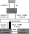
\includegraphics[width=14em]{\chapterdirectory/figure/cmp_overview.pdf}
\caption{Overview}%
\label{fig:cache-coherence-cmps-overview}
\end{subfigure} &
\begin{subfigure}[t]{0.47\textwidth}
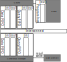
\includegraphics[width=20em]{\chapterdirectory/figure/cmp_detailed.pdf}
\caption{Showcasing the FIFOs}%
\label{fig:cache-coherence-cmps-fifos}
\end{subfigure}
\end{tabular}
\end{center}
\caption{Components involved in cache coherence}%
\label{fig:cache-coherence-cmps}
\end{figure}

In this section are presented the various components involved in maintaining
cache coherence in a multi-core architecture.
Figure~\ref{fig:cache-coherence-cmps} shows how the components presented in this
section are interconnected, with Figure~\ref{fig:cache-coherence-cmps-overview}
providing an overview and Figure~\ref{fig:cache-coherence-cmps-fifos} making
the involved FIFO queues more apparent.

Architectures generally feature instruction, data, as well as caches holding
both. Instruction caches are not affected by cache coherence and thus not
considered in this chapter.

\subsection{Memory Elements}%
\label{sec:memory_element}
The memory of a system is partitioned into addressable blocks. That is, there
are blocks of a certain size for which performing any access operation on its
content requires performing an operation on the block in its entirety.

Cache coherence is maintained over a cache line. Cache lines form another
partitioning of the system's main memory, such that all cache lines contain the
same amount of addressable blocks. Thus, even without accounting for the
possibility of multiple addresses pointing to the same atomic block, there may
be multiple addresses pointing to different parts of a same cache line. The
content of each cache line is made of contiguous memory blocks. Thus, if a
cache line of 16 elements starts with a block of address 42, it will also have
the blocks of addresses 43 through 57. If ignored, this mismatch between blocks
used for cache coherence and for program instructions can lead to unexpected
results, such as false sharing (see Appendix~\ref{app:false_sharing}).

To avoid unwarranted complications, this thesis merges the two partitioning
types into one: memory elements. In effect, we consider that memory elements
are cache lines with the size of a single addressable block, but change the
term so that this simplification remains explicit. Furthermore, since there is
only a single address per memory element, a memory element and its address can
be used interchangeably to refer to one another.

\begin{definition}[Memory Element]
\label{def:memoryelement}
The set of all memory elements is defined as $\memoryelements{} \subseteq
\mathbb{N}$.
\end{definition}

\subsection{Core: Programs \& Instructions}%
\label{sec:instructions}
Cache coherence is only affected by programs accessing the memory. As a result,
only the instructions related to the writing (\storeinstr{}), reading
(\loadinstr{}), and the eviction (\evictinstr{}) of memory elements are of any
considered while examining cache coherence. All other instructions are
assimilated into the no operation instruction (\nopinstr{}). As a result, when
observed through the lens of cache coherence, cores are executing programs by
adding instructions into a FIFO queue, without any possibility for branching or
jumping. Each of these instructions being applied to a single memory element.

The resolution of each instruction by its cache is signaled instantly to the
core, bypassing the need for a dedicated queue.

\begin{definition}[Instruction]
The set of all operators is defined as $\operators{} = \{\loadinstr{},
\storeinstr{}, \evictinstr{}, \nopinstr{}\}$, and instructions are defined
as $\instructions{} = \operators{} \times \memoryelements{}$
\end{definition}

\begin{definition}[Program]
Programs are sequences of instructions, thus $\programs{} =
\sequenceof{\instructions{}}$.
\end{definition}

\subsection{Caches}
\label{sec:cache_coherence:cache_cmp}
\begin{definition}[Cache]
\label{def:cache}
The set of all caches in the system is defined as \caches{}.  Some components
are present in both the caches and the coherence manager. We define
$\cachesandcmgr{} = \caches{} \cup \{\cmgr{}\}$ to add the coherence manager
(\cmgr{}). Furthermore, we define \nocache{}, not included in \caches{}, to
indicate the absence of a cache where one could be. The caches can also be
referred to using naturals from $1$ to \cachecount{}, with
$\cachecount{} = |\caches{}| - 1$.
\end{definition}

Caches are tasked with obtaining copies of memory elements able to fulfill the
memory accesses that are requested of them by their core. This requires keeping
track of permission for each copy of memory element they own, as well as
keeping track of operations (steps of the resolution of an instruction) that
are in progress. To do so, all caches assign a single state to each of their
memory element copies. These states are split into two categories:
\textit{stable} states, solely denoting that the cache has a certain permission
for that memory element, and \textit{transient} states, which indicate that the
resolution of a core's request is in progress and still awaiting either the
broadcast of a previously prepared query, or the reception of a data message
(or both).

\begin{definition}[States in Caches]
\label{def:cache_state}
\stablecachestate{} is the set of all stable states defined by the cache
coherence protocol, and \transientcachestate{} is the set of the transient
ones.  To shorten some notations, we also define $\cachestate{} =
\stablecachestate{} \cup \transientcachestate{}$, the set all cache states.
States cannot be both transient and stable, thus $\stablecachestate{} \cap
\transientcachestate{} = \emptyset$.
\end{definition}

To acquire new permissions, caches send queries on the interconnect. Each of
these queries pertains to a single memory element and leads to at most a single
reply being received by the emitter. For most types of data replies, a copy of
the memory element is part of the message. The types of queries that can be
sent are dependent on the actual cache coherence protocol. However, the
protocols used in this thesis all rely on the same ones: demand a read-only
copy of a memory element (\getsquery, likely following a \loadinstr{}
instruction), demand a read-and-write copy (\getmquery, likely following a
\storeinstr{} instruction), and signal the eviction of a potentially modified
copy (\putmquery, likely following an \evictinstr{}). Similarly, the
types of replies that can be exchanged are also dependent on the coherence
protocol. For those described in this thesis, only three types are required: a
message containing the memory element (\simpledata), one also indicating that
no other cache currently has access to that memory element (\exclusivedata),
and a message indicating that no copy of the memory element is going to be sent
(\nodata).

\begin{definition}[Query]
The categories of queries are defined as $\queries{} = \{\getsquery,
\getmquery, \putmquery\}$. A query message is an element of
$\querymessages{}: \queries{} \times \memoryelements{} \times \caches$, which
indicates the type of query, the memory element being targeted, and the
query's emitter.
\end{definition}

\begin{definition}[Reply]
The categories of reply messages are defined as $\replies{} = \{\simpledata,
\allowbreak{}
\exclusivedata,\allowbreak{} \nodata\}$. A reply message is an element of $\replymessages{}:
\replies{} \times \memoryelements{} \times \cachesandcmgr{}$, which indicates
its category, relevant memory element, and targeted cache (or \cmgr{}, when
targeting the coherence manager).
\end{definition}

Depending on what the cache coherence protocol allows, it is possible for
caches to receive queries they are in charge of replying to, despite not yet
having the data to do so. To handle such cases, caches can associate the
identifier of another cache with each address. By doing so, they are able to
send the data reply at a later date. As there is always at most one cache in
charge of providing a reply for any query, this can lead to caches waiting on a
reply, from a cache itself waiting on a reply, also receiving a query to which
they are supposed to be providing an answer. As the protocols ensure that there
is always exactly one component charged with replying for each memory element,
this cannot lead to a deadlock.

\begin{definition}[Information in Caches]
\label{def:cache_info}
Each cache associates a state to each memory element, and can also associate
with it the identifier of another cache. We define $\cachestatefun{} :
\caches{} \to \memoryelements{} \to \cachestate{}$ as the function indicating
the state associated with a given memory element by a given cache, and
$\replytofun{} : \caches{} \to \memoryelements{} \to (\caches{} \cup
\{\nocache{}\})$ is the function indicating the cache (or lack thereof)
expecting a data reply in the future for a given memory element in a given
cache.
\end{definition}

Each cache has four FIFO queues, each one handling either incoming or outgoing
queries or data messages, as seen in
Figure~\ref{fig:cache-coherence-cmps-fifos}.

\begin{definition}[Cache FIFOs]
\label{def:cache_fifos}
The four FIFOs of each cache are defined as:
$\cachedatainfun{} : \cachesandcmgr{} \to \sequenceof{\replymessages{}}$ and
$\cachedataoutfun{} : \cachesandcmgr{} \to \sequenceof{\replymessages{}}$ for the
incoming and outgoing data message queues;
$\cachequeryinfun{} : \cachesandcmgr{} \to \sequenceof{\querymessages{}}$ and
$\cachequeryoutfun{} : \caches{} \to \sequenceof{\querymessages{}}$ for the
incoming and outgoing query message queues.
\end{definition}

The behavior of a cache is described through a transition system focused on a
single memory element $E$ and reacting to events (Definition~\ref{def:event}).
The available actions within a transition for a cache $C$ are as follows:
\begin{itemize}
\item \textbf{Stalling:}
   stalling, written as \stallact{}, is a special action indicating that the
   event cannot be processed while the memory element is in this state. In
   effect, the event that led to this action being taken (be it an instruction
   from the core, an incoming query, or an incoming data message) is not
   removed from its queue and stays ready to be re-evaluated in any state where
   \stallact{} is no longer an action it leads to.

\item \textbf{Completing a core's request:}
   the \hitact{} indicates the cache has fulfilled one of its core's ongoing
   request for $E$. In some cases, multiple requests of different types
   (\loadinstr{}, \storeinstr{}, \evictinstr{}) may have be ongoing in
   parallel, leading the operator being fulfilled by the \hitact{} to be made
   explicit (e.g.~\storeinstr{} \hitact{}).

\item \textbf{Preparing a query:}
   a cache $C$ performing \sendqueryact{$Q$} is pushing a query of type $Q$ for
   the memory element $E$ in its outgoing query queue.
   \updatefun{\cachequeryoutfun{}}{C}{\pushfun{\langle{}Q, E,
   C\rangle{}}{\cachequeryoutfun{}(C)}}.

\item \textbf{Changing state:}
   The state attributed to $E$ is changed by writting \setstateact{$N$}, with
   $N$ being the new state. This corresponds to performing
   \updatefun{\cachestatefun{}}{C, E}{N}.

\item \textbf{Preparing a data reply:}
   when sending a data message, there are three possible targets: the emitter
   of an incoming query (\sendertarget{}), the coherence manager
   (\memorytarget{}), and a previously memorized cache (\replytotarget{}).
   \senddataact{$T$}{$D$} indicates that a data message of type $D$ is added to
   the outgoing data queue, with $T$ being its target.
   \updatefun{%
      \cachedataoutfun{}%
   }{C}{%
      \pushfun{\langle{}D, E, T\rangle{}}{%
         \cachedataoutfun{}(C)
      }
   }

\item \textbf{Memorizing a cache:}
   if an incoming query from $C_2$ is expected to be replied to by $C$, yet $C$
   is not currently able to provide data, the $C_2$ is memorized so that $C$
   knows to send data to $C_2$ when able. This is indicated by
   \storereplytoact{}, which is equivalent to $\updatefun{\replytofun{}}{C,
   E}{C_2}$. Although it does not impact the workings of cache coherence, the
   protocols shown in this thesis also indicate whenever the memorized cache
   can be cleared (\resetreplytoact{}, which is the same as
   \updatefun{\replytofun{}}{C, E}{\nocache{}}.
\end{itemize}

\subsection{Coherence Manager}
Maintaining cache coherence requires the caches to coordinate with each other.
Depending on the protocol, this may require some information to be accessible
to all caches. The coherence manager is a representation of this information.
This may not match any single one physical component of the system (for example
if there is no shared last level cache), as with certain protocols, its
behavior may be implemented through direct communication channels between the
caches. The role of the coherence manager is to act when none of the caches is
able to provide an answer to a cache's query. In order to detect such queries,
the coherence manager also assigns a state to each memory element. In effect,
the coherence manager acts as an intermediary between the caches and the
system's main memory. Furthermore, the coherence manager keeps track of which
cache, if any, is in charge of replying to queries.

\begin{definition}[Coherence Manager]
\label{def:cmgr_info}
Let \coherencemanagerstate{} the set of states that can be attributed by the
coherence manager, $\coherencemanagerstatefun{} : \memoryelements{} \to
\coherencemanagerstate{}$ is the function indicating which state is attributed
to each memory element. The cache (or lack thereof) associated with each memory
element is defined as $\coherencemanagerownerfun{} : \memoryelements{} \to
(\caches{} \cup \{\nocache{}\})$.
\end{definition}

Much like the caches, the coherence manager uses FIFO queues to handle incoming
and outgoing messages. It has one less queue however, as the coherence manager
never sends any query. This can be seen in Definition~\ref{def:cache_fifos},
where all but one of the types of FIFO queues are shared with the caches.

For a memory element $E$, the coherence manager's behavior can be defined
through the following actions:
\begin{itemize}
\item \textbf{Stalling:}
   the coherence manager may sometimes not be able to properly react to an
   incoming event. Just like caches, it can then use the special \stallact{}
   action to indicate that the event should not be processed while $E$ is in
   this state, leaving the event (either a query or a data message) untouched
   in its queue.

\item \textbf{Changing state:}
   as with the caches, the state attributed to $E$ by the coherence manager
   is changed by writing \setstateact{$N$}, with $N$ being the new state.
   This corresponds to \updatefun{\coherencemanagerstatefun{}}{E}{N}.

\item \textbf{Preparing a data reply:}
   the coherence manager replies to incoming cache queries by sending data.
   With the cache that emitted the query being referred to as \sendertarget{},
   the coherence manager can send a data message of type $D$ by performing
   \senddataact{$T$}{$D$}. This is equivalent to
   \updatefun{%
      \cachedataoutfun{}%
   }{\cmgr{}}{%
      \pushfun{\langle{}D, E, T\rangle{}}{%
         \cachedataoutfun{}(\cmgr{})
      }
   }

\item \textbf{Memorizing the current owner:}
   the coherence manager keeps track of which cache is currently in charge of
   distributing data for each memory element, if there is one. Similarly to the
   memorizing of a cache by another, having a cache $C_2$ be considered to have
   this role is done by \storeowneract{}, which corresponds to
   \updatefun{\coherencemanagerownerfun{}}{E}{C_2}. This value can also be
   cleared by having $C_2$ = \nocache{}.
\end{itemize}

\subsection{Interconnect}
The interconnect links all caches together, as well as the coherence manager.
It broadcasts queries from the caches to all the components it is linked to,
including the original query emitter. The replies, however, are targeted, and
thus only received by a single component.

Transfers between components are not instantaneous. Instead, outgoing message
queues are used to wait for access to the interconnect to become available.
Conversely, the interconnect deposits messages in incoming message queues so
that it does not have to synchronize with each component. Depending on the
system, some restrictions on how the interconnect behave can be present.
Indeed, not only is there generally an access policy controlling the order in
which outgoing messages are being sent (Round-Robin being commonly used), but
it is also possible for the interconnect to not allow a new query to be
broadcasted until the previous one has been resolved (such interconnects are
called atomic), whereas other interconnects allow the interleaving of queries
(split-transaction, where data and query use separate channels). This thesis
focuses on split-transaction buses architectures, as atomic buses are not found
in contemporary architectures.

In effect, the actions performed by the transitions of an automaton
corresponding to the interconnect are as follows:
\begin{itemize}
\item \textbf{Query Broadcast:}
   Given a cache $C_0$ such that $\neg\isemptyfun{\cachequeryoutfun{}(C_0)}$, a
   query broadcast takes a query $Q$ out of $C_0$'s outgoing query queue ($Q =
   \popfun{\cachequeryoutfun{}(C_0)}$) and adds it to every incoming query
   queues, including $C_0$'s (%
   $\updatefun{\cachequeryoutfun{}}{C_1}{\pushfun{Q}{\cachequeryoutfun{}(C_1)}}$).

\item \textbf{Data Transfer:}
   Given $C_0$, either a cache or the coherence manager, such that
   $\neg\isemptyfun{\cachedataoutfun{}(C_0)}$, a data transfer for
   $\langle{}D, E, T\rangle{} = \popfun{\cachedataoutfun{}(C_0)}$ adds the
   corresponding data message to $T$'s incoming data messages queue (%
   $\updatefun{%
      \cachedatainfun{}%
   }{T}{%
      \pushfun{\langle{}D, E, T\rangle{}}{%
         \cachedatainfun{}(T)
      }
   }$).
\end{itemize}

\stopallthesefloats{}
\section{Coherence Protocols}
When definiting the protocols, the behavior of the caches and the coherence
manager is given in the form of a classical automata (see
Chapter~\ref{cha:formal_methods}), and limited to a single memory component.

\subsection{Introduction to the MSI Protocol}
\label{sec:intro_to_msi}
The archetypal cache coherence protocols are those belonging to the MSI
protocol family. In their basic version, these protocols feature three stable
states from which the MSI name is derived:
\begin{itemize}
\item \textbf{Modified:}
When a cache assigns the Modified state to a memory element, it indicates that
this cache performed at least one write to that memory element. While in this
state, it can freely read and write to that memory element. This corresponds
to being the \textit{Single Writer} from Property~\ref{prop:swmr}.

\item \textbf{Shared:}
When a cache assigns the Shared state to a memory element, it indicates that
this cache is able to freely read that memory element but not write to it. This
corresponds to being one of the \textit{Multiple Readers} (and potentially the
only one) of Property~\ref{prop:swmr}.

\item \textbf{Invalid:}
When a cache assigns the Invalid state to a memory element, it is no longer
considered to be holding a copy of that memory element, thus absolving this
cache from verifying Property~\ref{prop:system_wide_value}. Not having a copy,
the cache can neither read nor write to the memory element.
\end{itemize}

\stopallthesefloats
\begin{figure}
   \begin{center}
   \begin{subfigure}[b]{0.7\linewidth}
      \input{\chapterdirectory/figure/general_msi_cc}
      \caption{Cache}
      \label{fig:general_msi_cc}
   \end{subfigure}
   \\
   \begin{subfigure}[b]{0.5\linewidth}
      \input{\chapterdirectory/figure/general_msi_cmgr}
      \caption{Coherence Manager}
      \label{fig:general_msi_cmgr}
   \end{subfigure}
   \begin{subfigure}[b]{0.3\linewidth}
      \input{\chapterdirectory/figure/general_msi_cpu}
      \caption{Core}
      \label{fig:general_msi_cpu}
   \end{subfigure}
   \end{center}
   \caption{Overview of the MSI Protocol}
   \label{fig:general_msi}
\end{figure}

To keep it simple, the protocol presented in this section does not use any FIFO
queue. Instead, all exchanges are done synchronously. The only elements taken
into account are the state of the memory elements and the points of
synchronization (i.e. instruction and message exchanges). Thus, the notations
on the automata of this section are not the notations presented in the previous
section, but are instead based on CCS (Calculus of Communicating Systems,
\cite{10.5555/539036}): a \texttt{?} marks the reception of a signal, and
\texttt{!} marks its sending.  Queries are still sent to all components, and
data only to a single one.  Furthermore, only a single transaction (that is,
the resolution of an instruction) can occur at any
moment. This is reflected by transitions featuring multiple synchronizations,
as no other actions would be permitted to be interleaved.

Figure~\ref{fig:general_msi} shows the two automata corresponding to this
simplified protocol. Each of these automata pertains to a single memory element,
with states corresponding to what the component attributes to that memory
element.

In the case of the coherence manager (Figure~\ref{fig:general_msi_cmgr}), the
two states simply correspond to whether or not the coherence manager is in
charge of providing the current value for that memory element: \texttt{M}
indicates that one of the caches is currently in the \texttt{M} state, meaning
that the value stored in the system's main memory may be out of date; \texttt{I}
indicates that the main memory's value for that element is up-to-date, leaving
(in the MSI protocol) the coherence manager in charge of propagating copies
as the caches demand them.

\begin{example}[Simple MSI Transition]
\label{ex:general_msi_single_store}
Consider a system with two caches, $C_A$ and $C_B$, and a single memory
element $E$, such that, initially, $C_A$ holds no copy of $E$ (\texttt{I}
state) and $C_B$ holds one in the \texttt{S} state, the coherence manager
has the \texttt{I} state assigned to $E$. Were $C_A$ to receive a \storeinstr{}
request, it would broadcast a \getmquery{} to itself, $C_B$, and the coherence
manager. Upon receiving the \getmquery{}, $C_B$ would have to abandon the
\texttt{S} state for \texttt{I} in order to maintain Property~\ref{prop:swmr}.
The coherence manager would react to receiving the \getmquery{} by sending a
copy of $E$ from the system's main memory to $C_A$ (\simpledata!)
before moving to \texttt{M} so as to memorize that the most up-to-date value
for $E$ is now held by $C_A$. This \simpledata{} reply allows $C_A$ to move to
the \texttt{M} state, thus completing its transition.
\end{example}



\subsection{Properties to be Verified}
\label{sec:proper_cache_coherence_protocol}
A system maintaining cache coherence is a system in which the application of
each read and write instruction on the same memory elements across multiple
caches holds the same results as if these caches shared a permanent single copy
of each of those memory elements.

One possible strategy to achieve cache coherence is to enforce
Properties~\ref{prop:system_wide_value}, \ref{prop:swmr}, and
\ref{prop:forget_me_not}. Other approaches may also be possible, but this is
the one considered in this thesis.

\begin{property}[Caches Have the System-Wide Value]%
\label{prop:system_wide_value}
At any point, for each memory element, all copies of that memory element being
held in a cache have the value that was last written to that memory element,
regardless of which cache performed the writing.
\end{property}

\begin{property}[Single Writer or Multiple Readers]%
\label{prop:swmr}
At any point, for each memory element, there is either a single cache being
able to write to that memory element while the others can neither read nor
write to it, or there is any number of caches being able to read the memory
element and none able to write to it.
\end{property}

\begin{property}[Forget Me Not]%
\label{prop:forget_me_not}
If a memory element has no copy held in cache, then the system's main memory
has the value that was last written to that memory element.
\end{property}

Cache coherence protocols can be split into categories according to whether
they are directory-based or snooping-based, and write-back or write-through.

As this thesis only considers snooping-based protocols, the component
descriptions provided in Section~\ref{sec:cache_coherence_components} are
unlikely to fit a directory-based protocol. Indeed, in directory-based
protocols, cache queries are not broadcasted to every cache but instead
addressed to a component that, much like the coherence manager, keeps track of
which component may need to see this query and sends a copy of that query to
them. In snooping-based protocols, the caches and the coherence manager all
receive every query, and do so in the same order.

Write-through protocols ensure that any modification made to a memory element's
copy in a cache is also applied to the original in the system's main memory.
Conversely, write-back protocols delay the modification of the original until
the cache loses the write permissions on its own copy. As it happens, the
protocols studied during this thesis are all write-back ones.

\subsection{Protocol Definition}
Protocols are customarily defined by the behavior they require of caches (and
the coherence manager, if it is used) for a single memory element according to
its currently attributed state in the component and the type of incoming event.

\begin{definition}[Event]
\label{def:event}
Events for a single memory element are defined as $\events{} = \querymessages{}
\cup \instructions{} \cup \replymessages{}$
%\cup \{\ownquery{}\}$, with \ownquery{} indicating a query that was sent by this cache.
\end{definition}

\begin{definition}[Protocol]
\label{def:protocol}
A protocol is thus defined as two functions:
$\protocolccfun{} = \cachestate \to \events{} \to set(\actions{})$, which
defines the behavior of cache controllers, given the state of memory element
and an incoming event; and
$\protocolcmgrfun{} = \coherencemanagerstate \to \events{} \to set(\actions{})$,
the coherence manager equivalent. \actions{} corresponds to the actions
described in each component's sub-section.
\end{definition}

\begin{definition}[System State]
\label{def:systemstate}
   For the definition of a cache coherence protocol, only a single memory
   element needs to be considered. Indeed, the behavior is the same for any
   address, and thus defining it for one is defining it for all. This can be
   exploited to shorthand the notation of memory element states across the
   system: Given $E$ the memory element arbitrarily chosen for the protocol's
   definition, a system $\langle CC_1, \ldots, CC_n, CM\rangle$ denotes one in
   which
   $
      \coherencemanagerstatefun{}(E) = CM \land
      \forallin{c}{0..\cachecount}{%
         \cachestatefun(c, E) = CC_c
      }
   $. The set of all possible systems states is denoted \systemstate{}.
\end{definition}

\begin{definition}[Stable System Transitions]
   \label{def:hypreachfun}
   To allow reasoning more simply over state changes, another shorthand notation
   is introduced: $\hypreachfun{}: \systemstate{} \to
   \instructions{}^\cachecount{} \to set(\systemstate{})$ which, given a system
   state and instructions to apply on each cache, returns the set of all
   possible next system states composed solely of stable states that can be
   reached.
\end{definition}

\stopallthesefloats{}
\section{Split-Transaction Bus, case of the MSI Protocol}
\label{sec:split_msi}
Section~\ref{sec:intro_to_msi} provides an overview of the MSI protocol without
considerations for the possibility of interleaving or even asynchronous
communications. This section presents an MSI protocol featuring all of those.
This leads a large number of additional states and transitions, so instead of
using graphs to represent the automata, we use matrices (see
Figure~\ref{fig:msi_cc_table} for the cache controllers, and
Figure~\ref{fig:msi_mgr_table} for the coherence manager). The columns in
these matrices correspond to the events from Definition~\ref{def:event}. Bear
in mind that this corresponds to how the caches and the coherence manager act
for each memory element, according to the state currently assigned to that
state (first column). The \textbf{Own Query} column in the cache's
table corresponds to when it processes one of its own queries (from its incoming
query queue) for that memory element. In the coherence manager's table, the
behavior upon reception of a query may differ according to whether the emitter
is the owner (as defined by the \coherencemanagerownerfun{} function) or not.

\subsection{State Naming}
\label{sec:cache_state_naming}
Invalid (\texttt{I}), Shared (\texttt{S}), and Modified (\texttt{M}) are the
three stable states of the \texttt{MSI} protocol, the other states are
transient.

Reception of a request that requires use of the interconnect will usually lead
to a \texttt{XY\textsuperscript{BD}} transient state, which means that the
cache controller is handling a transition between the stable states \texttt{X}
and \texttt{Y}, with \textsuperscript{B} indicating that this transition
requires the acquisition of the interconnect and \textsuperscript{D} the
reception of a related data reply (regardless of whether it comes from an other
cache controller or the memory).

\texttt{XY\textsuperscript{D}} usually follows \texttt{XY\textsuperscript{BD}}
if the cache controller sees its own query before receiving a reply. If the
reply is seen first, then the memory element goes into the
\texttt{XY\textsuperscript{B}} state instead. While the former is more likely,
the latter may occur because, despite processing all queries in the same order,
not all cache controllers take the same time to do so.

It is also possible an external query to lead to a change of state, especially
when in the \texttt{XY\textsuperscript{D}} state. Indeed, at that point, the
system pretty much considers that the cache controller is in the \texttt{Y}
state, and thus has the responsibilities that the \texttt{Y} state would imply.
This makes it possible for a cache controller to see a query it needs to act
upon before being actually ready to do so (e.g.~observing a \texttt{GetM} query
while waiting for \texttt{data}). The states thus reached have either a
\texttt{XY\textsuperscript{D}V} pattern, with \texttt{V} being a stable state,
indicating that the external query would have required this memory element to be
assigned the \texttt{V} state if it were currently in the \texttt{Y} state.
Thus, this state is used to memorize that, after sending the data, the cache is
expected to perform the appropriate change of state. It is possible for
the \texttt{Y} state to also be susceptible to external queries. Thus, there
are also \texttt{XY\textsuperscript{D}YZ} states, indicating that the final
state is now \texttt{Z}.

\begin{figure}
\begin{center}
\begin{tabular}{|l||c|c|c|c|c||c|c|c|}
 \hline

 \textbf{State}
 & \multicolumn{3}{c|}{\textbf{Core Request}}
 & \begin{tabular}{@{}c@{}}
      \textbf{Own}\\
      \textbf{Query}
   \end{tabular}
 & \begin{tabular}{@{}c@{}}
      \textbf{Data}\\
      \textbf{Reply}
   \end{tabular}
 & \multicolumn{3}{c|}{\textbf{Received Queries}}
 \\

%%%%%%%%%%%%%%%%%%%%%%%%%%%%%%%%%%%%%%%%%%%%%%%%%%%%%%%%%%%%%%%%%%%%%%%%%%%%%%%%
 & \loadinstr{} & \storeinstr{} & \evictinstr{}
 &
 &
 & \getsquery{} & \getmquery{} & \putmquery{}
 \\
 \hline

%%%%%%%%%%%%%%%%%%%%%%%%%%%%%%%%%%%%%%%%%%%%%%%%%%%%%%%%%%%%%%%%%%%%%%%%%%%%%%%%
 \texttt{I}

 % Load/Store/Evict
 &
   \begin{tabular}{@{}c@{}}
      \sendqueryact{\getsquery{}}\\
      \setstateact{\texttt{IS\textsuperscript{BD}}}
   \end{tabular}
 &
   \begin{tabular}{@{}c@{}}
      \sendqueryact{\getmquery{}}\\
      \setstateact{\texttt{IM\textsuperscript{BD}}}
   \end{tabular}
 & \disablecell{}

 % Seeing Own Query
 & \disablecell{}

 % Data Reply
 & \disablecell{}

 % GetS/GetM/PutM
 & \noaction{}
 & \noaction{}
 & \noaction{}
 \\
 \hline

%%%%%%%%%%%%%%%%%%%%%%%%%%%%%%%%%%%%%%%%%%%%%%%%%%%%%%%%%%%%%%%%%%%%%%%%%%%%%%%%
 \texttt{IS\textsuperscript{BD}}

 % Load/Store/Evict
 & \stallact{}
 & \stallact{}
 & \stallact{}

 % Seeing Own Query
 & \setstateact{\texttt{IS\textsuperscript{D}}}

 % Data Reply
 & \setstateact{\texttt{IS\textsuperscript{B}}}

 % GetS/GetM/PutM
 & \noaction{}
 & \noaction{}
 & \noaction{}
 \\
 \hline

%%%%%%%%%%%%%%%%%%%%%%%%%%%%%%%%%%%%%%%%%%%%%%%%%%%%%%%%%%%%%%%%%%%%%%%%%%%%%%%%
 \texttt{IS\textsuperscript{B}}

 % Load/Store/Evict
 & \stallact{}
 & \stallact{}
 & \stallact{}

 % Seeing Own Query
 & \setstateact{\texttt{S}}

 % Data Reply
 & \disablecell{}

 % GetS/GetM/PutM
 & \noaction{}
 & \noaction
 & \disablecell{}
 \\
 \hline

%%%%%%%%%%%%%%%%%%%%%%%%%%%%%%%%%%%%%%%%%%%%%%%%%%%%%%%%%%%%%%%%%%%%%%%%%%%%%%%%
 \texttt{IS\textsuperscript{D}}

 % Load/Store/Evict
 & \stallact{}
 & \stallact{}
 & \stallact{}

 % Seeing Own Query
 & \disablecell{}

 % Data Reply
 & \setstateact{\texttt{S}}

 % GetS/GetM/PutM
 & \noaction{}
 & \setstateact{\texttt{IS\textsuperscript{D}I}}
 & \disablecell{}
 \\
 \hline

%%%%%%%%%%%%%%%%%%%%%%%%%%%%%%%%%%%%%%%%%%%%%%%%%%%%%%%%%%%%%%%%%%%%%%%%%%%%%%%%
 \texttt{IS\textsuperscript{D}I}

 % Load/Store/Evict
 & \stallact{}
 & \stallact{}
 & \stallact{}

 % Seeing Own Query
 & \disablecell{}

 % Data Reply
 & \setstateact{\texttt{I}}

 % GetS/GetM/PutM
 & \noaction{}
 & \noaction{}
 & \disablecell{}
 \\
 \hline

%%%%%%%%%%%%%%%%%%%%%%%%%%%%%%%%%%%%%%%%%%%%%%%%%%%%%%%%%%%%%%%%%%%%%%%%%%%%%%%%
 \texttt{IM\textsuperscript{BD}}

 % Load/Store/Evict
 & \stallact{}
 & \stallact{}
 & \stallact{}

 % Seeing Own Query
 & \setstateact{\texttt{IM\textsuperscript{D}}}

 % Data Reply
 & \setstateact{\texttt{IM\textsuperscript{B}}}

 % GetS/GetM/PutM
 & \noaction{}
 & \noaction{}
 & \noaction{}
 \\
 \hline

%%%%%%%%%%%%%%%%%%%%%%%%%%%%%%%%%%%%%%%%%%%%%%%%%%%%%%%%%%%%%%%%%%%%%%%%%%%%%%%%
 \texttt{IM\textsuperscript{B}}

 % Load/Store/Evict
 & \stallact{}
 & \stallact{}
 & \stallact{}

 % Seeing Own Query
 & \setstateact{\texttt{M}}

 % Data Reply
 & \disablecell{}

 % GetS/GetM/PutM
 & \noaction{}
 & \noaction{}
 & \noaction{}
 \\
 \hline

%%%%%%%%%%%%%%%%%%%%%%%%%%%%%%%%%%%%%%%%%%%%%%%%%%%%%%%%%%%%%%%%%%%%%%%%%%%%%%%%
 \texttt{IM\textsuperscript{D}}

 % Load/Store/Evict
 & \stallact{}
 & \stallact{}
 & \stallact{}

 % Seeing Own Query
 & \disablecell{}

 % Data Reply
 & \setstateact{\texttt{M}}

 % GetS/GetM/PutM
 & \begin{tabular}{@{}c@{}}
      \storereplytoact{}\\
      \setstateact{\texttt{IM\textsuperscript{D}S}}
   \end{tabular}
 & \begin{tabular}{@{}c@{}}
      \storereplytoact{}\\
      \setstateact{\texttt{IM\textsuperscript{D}I}}
   \end{tabular}
 & \disablecell{}
 \\
 \hline

%%%%%%%%%%%%%%%%%%%%%%%%%%%%%%%%%%%%%%%%%%%%%%%%%%%%%%%%%%%%%%%%%%%%%%%%%%%%%%%%
 \texttt{IM\textsuperscript{D}I}

 % Load/Store/Evict
 & \stallact{}
 & \stallact{}
 & \stallact{}

 % Seeing Own Query
 & \disablecell{}

 % Data Reply
 &
   \begin{tabular}{@{}c@{}}
      \senddataact{\replytotarget{}}{\simpledata{}}\\
      \setstateact{\texttt{I}}
   \end{tabular}

 % GetS/GetM/PutM
 & \noaction{}
 & \noaction{}
 & \disablecell{}
 \\
 \hline

%%%%%%%%%%%%%%%%%%%%%%%%%%%%%%%%%%%%%%%%%%%%%%%%%%%%%%%%%%%%%%%%%%%%%%%%%%%%%%%%
 \texttt{IM\textsuperscript{D}S}

 % Load/Store/Evict
 & \stallact{}
 & \stallact{}
 & \stallact{}

 % Seeing Own Query
 & \disablecell{}

 % Data Reply
 & \begin{tabular}{@{}c@{}}
      \senddataact{\replytotarget{}}{\simpledata{}}\\
      \senddataact{\memorytarget{}}{\simpledata{}}\\
      \setstateact{\texttt{I}}
   \end{tabular}

 % GetS/GetM/PutM
 & \noaction{}
 & \setstateact{\texttt{IM\textsuperscript{D}SI}}
 & \disablecell{}
 \\
 \hline

%%%%%%%%%%%%%%%%%%%%%%%%%%%%%%%%%%%%%%%%%%%%%%%%%%%%%%%%%%%%%%%%%%%%%%%%%%%%%%%%
 \texttt{IM\textsuperscript{D}SI}

 % Load/Store/Evict
 & \stallact{}
 & \stallact{}
 & \stallact{}

 % Seeing Own Query
 & \disablecell{}

 % Data Reply
 & \begin{tabular}{@{}c@{}}
      \senddataact{\replytotarget{}}{\simpledata{}}\\
      \senddataact{\memorytarget{}}{\simpledata{}}\\
      \setstateact{\texttt{I}}
   \end{tabular}

 % GetS/GetM/PutM
 & \noaction{}
 & \noaction{}
 & \disablecell{}
 \\
 \hline

%%%%%%%%%%%%%%%%%%%%%%%%%%%%%%%%%%%%%%%%%%%%%%%%%%%%%%%%%%%%%%%%%%%%%%%%%%%%%%%%
 \texttt{S}

 % Load/Store/Evict
 & \hitact{}
 &
   \begin{tabular}{@{}c@{}}
      \sendqueryact{\getmquery{}}\\
      \setstateact{\texttt{SM\textsuperscript{BD}}}
   \end{tabular}
 & \setstateact{\texttt{I}}

 % Seeing Own Query
 & \disablecell{}

 % Data Reply
 & \disablecell{}

 % GetS/GetM/PutM
 & \noaction{}
 & \setstateact{\texttt{I}}
 & \disablecell{}
 \\
 \hline

%%%%%%%%%%%%%%%%%%%%%%%%%%%%%%%%%%%%%%%%%%%%%%%%%%%%%%%%%%%%%%%%%%%%%%%%%%%%%%%%
 \texttt{SM\textsuperscript{BD}}

 % Load/Store/Evict
 & \hitact{}
 & \stallact{}
 & \stallact{}

 % Seeing Own Query
 & \setstateact{\texttt{SM\textsuperscript{D}}}

 % Data Reply
 & \setstateact{\texttt{SM\textsuperscript{B}}}

 % GetS/GetM/PutM
 & \noaction{}
 & \setstateact{\texttt{IM\textsuperscript{BD}}}
 & \disablecell{}
 \\
 \hline

%%%%%%%%%%%%%%%%%%%%%%%%%%%%%%%%%%%%%%%%%%%%%%%%%%%%%%%%%%%%%%%%%%%%%%%%%%%%%%%%
 \texttt{SM\textsuperscript{B}}

 % Load/Store/Evict
 & \hitact{}
 & \stallact{}
 & \stallact{}

 % Seeing Own Query
 & \setstateact{\texttt{M}}

 % Data Reply
 & \disablecell{}

 % GetS/GetM/PutM
 & \noaction{}
 & \setstateact{\texttt{IM\textsuperscript{B}}}
 & \disablecell{}
 \\
 \hline


%%%%%%%%%%%%%%%%%%%%%%%%%%%%%%%%%%%%%%%%%%%%%%%%%%%%%%%%%%%%%%%%%%%%%%%%%%%%%%%%
 \texttt{SM\textsuperscript{D}}

 % Load/Store/Evict
 & \hitact{}
 & \stallact{}
 & \stallact{}

 % Seeing Own Query
 & \disablecell{}

 % Data Reply
 & \setstateact{\texttt{M}}

 % GetS/GetM/PutM
 & \begin{tabular}{@{}c@{}}
      \senddataact{\replytotarget{}}{\simpledata{}}\\
      \setstateact{\texttt{SM\textsuperscript{D}S}}
   \end{tabular}
 & \begin{tabular}{@{}c@{}}
      \senddataact{\replytotarget{}}{\simpledata{}}\\
      \setstateact{\texttt{SM\textsuperscript{D}I}}
   \end{tabular}
 & \disablecell{}
 \\
 \hline

%%%%%%%%%%%%%%%%%%%%%%%%%%%%%%%%%%%%%%%%%%%%%%%%%%%%%%%%%%%%%%%%%%%%%%%%%%%%%%%%
 \texttt{SM\textsuperscript{D}I}

 % Load/Store/Evict
 & \hitact{}
 & \stallact{}
 & \stallact{}

 % Seeing Own Query
 & \disablecell{}

 % Data Reply
 & \begin{tabular}{@{}c@{}}
      \senddataact{\replytotarget{}}{\simpledata{}}\\
      \setstateact{\texttt{I}}
   \end{tabular}

 % GetS/GetM/PutM
 & \noaction{}
 & \noaction{}
 & \disablecell{}
 \\
 \hline

%%%%%%%%%%%%%%%%%%%%%%%%%%%%%%%%%%%%%%%%%%%%%%%%%%%%%%%%%%%%%%%%%%%%%%%%%%%%%%%%
 \texttt{SM\textsuperscript{D}S}

 % Load/Store/Evict
 & \hitact{}
 & \stallact{}
 & \stallact{}

 % Seeing Own Query
 & \disablecell{}

 % Data Reply
 & \begin{tabular}{@{}c@{}}
      \senddataact{\replytotarget{}}{\simpledata{}}\\
      \senddataact{\memorytarget{}}{\simpledata{}}\\
      \setstateact{\texttt{S}}
   \end{tabular}

 % GetS/GetM/PutM
 & \noaction{}
 & \setstateact{\texttt{SM\textsuperscript{D}SI}}
 & \disablecell{}
 \\
 \hline

%%%%%%%%%%%%%%%%%%%%%%%%%%%%%%%%%%%%%%%%%%%%%%%%%%%%%%%%%%%%%%%%%%%%%%%%%%%%%%%%
 \texttt{SM\textsuperscript{D}SI}

 % Load/Store/Evict
 & \hitact{}
 & \stallact{}
 & \stallact{}

 % Seeing Own Query
 & \disablecell{}

 % Data Reply
 & \begin{tabular}{@{}c@{}}
      \senddataact{\replytotarget{}}{\simpledata{}}\\
      \senddataact{\memorytarget{}}{\simpledata{}}\\
      \setstateact{\texttt{I}}
   \end{tabular}

 % GetS/GetM/PutM
 & \noaction{}
 & \noaction{}
 & \disablecell{}
 \\
 \hline

%%%%%%%%%%%%%%%%%%%%%%%%%%%%%%%%%%%%%%%%%%%%%%%%%%%%%%%%%%%%%%%%%%%%%%%%%%%%%%%%
 \texttt{M}

 % Load/Store/Evict
 & \hitact{}
 & \hitact{}
 & \begin{tabular}{@{}c@{}}
      \sendqueryact{\putmquery{}}\\
      \setstateact{\texttt{MI\textsuperscript{B}}}
   \end{tabular}

 % Seeing Own Query
 & \disablecell{}

 % Data Reply
 & \disablecell{}

 % GetS/GetM/PutM
 &
   \begin{tabular}{@{}c@{}}
      \senddataact{\memorytarget{}}{\simpledata{}}\\
      \senddataact{\sendertarget{}}{\simpledata{}}\\
      \setstateact{\texttt{S}}
   \end{tabular}
 &
   \begin{tabular}{@{}c@{}}
      \senddataact{\sendertarget{}}{\simpledata{}}\\
      \setstateact{\texttt{I}}
   \end{tabular}
 & \disablecell{}
 \\
 \hline

%%%%%%%%%%%%%%%%%%%%%%%%%%%%%%%%%%%%%%%%%%%%%%%%%%%%%%%%%%%%%%%%%%%%%%%%%%%%%%%%
 \texttt{MI\textsuperscript{B}}

 % Load/Store/Evict
 & \hitact{}
 & \hitact{}
 & \stallact{}

 % Seeing Own Query
 &
   \begin{tabular}{@{}c@{}}
      \senddataact{\memorytarget{}}{\simpledata{}}\\
      \setstateact{\texttt{I}}
   \end{tabular}

 % Data Reply
 & \disablecell{}

 % GetS/GetM/PutM
 &
   \begin{tabular}{@{}c@{}}
      \senddataact{\memorytarget{}}{\simpledata{}}\\
      \senddataact{\sendertarget{}}{\simpledata{}}\\
      \setstateact{\texttt{II\textsuperscript{B}}}
   \end{tabular}
 &
   \begin{tabular}{@{}c@{}}
      \senddataact{\sendertarget{}}{\simpledata{}}\\
      \setstateact{\texttt{II\textsuperscript{B}}}
   \end{tabular}
 & \disablecell{}
 \\
 \hline

%%%%%%%%%%%%%%%%%%%%%%%%%%%%%%%%%%%%%%%%%%%%%%%%%%%%%%%%%%%%%%%%%%%%%%%%%%%%%%%%
 \texttt{II\textsuperscript{B}}

 % Load/Store/Evict
 & \stallact{}
 & \stallact{}
 & \stallact{}

 % Seeing Own Query
 & \setstateact{\texttt{I}}

 % Data Reply
 & \disablecell{}

 % GetS/GetM/PutM
 & \noaction{}
 & \noaction{}
 & \noaction{}
 \\
 \hline

 \multicolumn{1}{l|}{}
 & \multicolumn{5}{c||}{\textbf{Handling Requests}}
 & \multicolumn{3}{c|}{\textbf{Handling Queries}}
 \\
 \cline{2-9}
\end{tabular}

\end{center}
\caption{Split-Transaction MSI Automaton for Cache Controllers}
\label{fig:msi_cc_table}
\end{figure}
%
%Figure~\ref{fig:msi_mgr_table} shows how the coherency manager keeps track of
%whether the RAM has the most up-to-date value for a memory element (state
%\texttt{I}) or if a cache controller does (state \texttt{M}). This is used to
%determine if the RAM should be the one to reply when either a \texttt{GetS} or a
%\texttt{GetM} query passes through the interconnect. The \texttt{I} state
%indicates that the RAM currently has the most up-to-date value. The
%\texttt{I\textsuperscript{D}} state indicates that the RAM should be the one to
%respond to queries, but it still hasn't received the latest value.  Unlike the
%cache controller, it will not switch to a dedicated state but instead force
%queries from the interconnect to stall until the problematic query can be
%fulfilled. \texttt{I\textsuperscript{B}} indicates that the RAM has received
%the latest value, but has not yet seen the query that led this data to be sent.

\begin{figure}
\begin{center}
\input{\chapterdirectory/figure/split_msi_coherence_manager.tex}
\end{center}
\caption{Split-Transaction MSI Automaton for Coherence Manager}
\label{fig:msi_mgr_table}
\end{figure}

\stopallthesefloats
\subsection{Examples}
\stopallthesefloats
\begin{example}[Simple Read]
\label{ex:split_msi_simple_read}
In this example a single cache is moving from not having any access to a
memory element to having a read-only copy. This is one the simplest example of
transaction and is meant to show how messages are exchanged. This example is
illustrated as a sequence in Figure~\ref{fig:split_msi_simple_read}.

\begin{figure}[h!bt]
\begin{center}
\begin{tabular}{ccc}
\begin{subfigure}[t]{0.3\textwidth}
\includegraphics[width=\columnwidth]{\chapterdirectory/figure/i_to_s_alone_demo/f00.pdf}
\caption{%
$C_A$ holds the memory element in the \texttt{I} state. As no cache holds any
copy, its value must be provided by the main memory. Thus, $C_{mgr}$ considers
the memory element to be in the \texttt{I} state.
}
\end{subfigure} &

\begin{subfigure}[t]{0.3\textwidth}
\includegraphics[width=\columnwidth]{\chapterdirectory/figure/i_to_s_alone_demo/f01.pdf}
\caption{%
$C_A$'s core now issues a \texttt{load} instruction on $42$.  This leads $C_A$
to move to the \texttt{IS\textsuperscript{BD}} state, and to prepare a
\texttt{GetS} query in its outgoing query queue.
}
\end{subfigure} &

\begin{subfigure}[t]{0.3\textwidth}
\includegraphics[width=\columnwidth]{\chapterdirectory/figure/i_to_s_alone_demo/f02.pdf}
\caption{%
The interconnect broadcasts outgoing queries from caches to all the incoming
query queues: $C_A$'s \texttt{GetS} is added to both its own and $C_{mgr}$'s
incoming query queue.
}
\end{subfigure}
\end{tabular}
\end{center}
\end{figure}

\begin{figure}\ContinuedFloat
\begin{center}
\begin{tabular}{ccc}
\begin{subfigure}[t]{0.3\textwidth}
\includegraphics[width=\columnwidth]{\chapterdirectory/figure/i_to_s_alone_demo/f03.pdf}
\caption{%
Consuming the message in its incoming query queue, $C_A$ confirms it has
processed all other prior queries and now associates the
\texttt{IS\textsuperscript{D}} state to $42$, which indicates that a data reply
is now expected. Similarly, $C_{mgr}$ consumes the \texttt{GetS} query, and,
since the main memory is in charge of replying prepares a data message for
$C_A$.
}
\end{subfigure} &

\begin{subfigure}[t]{0.3\textwidth}
\centering
\includegraphics[width=\columnwidth]{\chapterdirectory/figure/i_to_s_alone_demo/f04.pdf}
\caption{%
The interconnect transfers the data message from $C_{mgr}$ to $C_A$.
}
\end{subfigure} &

\begin{subfigure}[t]{0.3\textwidth}
\includegraphics[width=\columnwidth]{\chapterdirectory/figure/i_to_s_alone_demo/f05.pdf}
\caption{%
By receiving the data message, $C_A$ has obtained a read-only copy of $42$,
making it switch to the \texttt{S} state and completing its core's request.
}
\end{subfigure}
\end{tabular}
\end{center}
\caption{Illustrations for \textbf{Simple Read}}
\label{fig:split_msi_simple_read}
\end{figure}
\end{example}


\stopallthesefloats
\begin{example}[Reaching \texttt{S}]
\label{ex:split_msi_reaching_s}
This example is meant to showcase how exchanges between cache controllers are
assumed to take place. To keep things simple, we only consider two cores and a
single memory element (whose address is $42$). This example is illustrated as a
sequence in Figure~\ref{fig:split_msi_reach_s}.

\begin{figure}[h!bt]
\begin{center}
\begin{tabular}{cc}
\begin{subfigure}[t]{0.47\textwidth}
\includegraphics[width=\columnwidth]{\chapterdirectory/figure/i_to_s_demo/f00.pdf}
\caption{%
$C_A$ holds that memory element in the \texttt{I} state, while the
other, $C_B$, holds it in the \texttt{M} state. As $C_B$ may have modified the
memory element, $C_{mgr}$ considers the memory element to be in the \texttt{M}
state. Furthermore, $C_{mgr}$ has memorized that $C_B$ is currently in charge
of that particular memory element (\texttt{o:} $C_B$).
}
\end{subfigure} &

\begin{subfigure}[t]{0.47\textwidth}
\includegraphics[width=\columnwidth]{\chapterdirectory/figure/i_to_s_demo/f01.pdf}
\caption{%
Next, we consider that $C_A$'s core issued a \texttt{load} instruction on $42$.
This leads $C_A$ to move to the \texttt{IS\textsuperscript{BD}} state, and to
issue a \texttt{GetS} query to its outgoing query queue.
}
\end{subfigure}
\end{tabular}
\end{center}
\end{figure}

\begin{figure}\ContinuedFloat
\begin{center}
\begin{tabular}{cc}

\begin{subfigure}[t]{0.47\textwidth}
\includegraphics[width=\columnwidth]{\chapterdirectory/figure/i_to_s_demo/f02.pdf}
\caption{%
The interconnect broadcasts outgoing queries from caches to all the incoming
query queues. As $C_A$ is the only one with an outgoing query, the
\texttt{GetS} is added to both its own and $C_B$'s incoming query queue,
as well as the coherency manager's.
}
\end{subfigure} &

\begin{subfigure}[t]{0.47\textwidth}
\includegraphics[width=\columnwidth]{\chapterdirectory/figure/i_to_s_demo/f03.pdf}
\caption{%
Consuming the message in their incoming query queues, $C_A$, $C_B$
and $C_{mgr}$ change state, moving to \texttt{IS\textsuperscript{D}},
\texttt{S}, and \texttt{I\textsuperscript{D}} respectively. In addition, $C_B$
adds a reply for the query to its outgoing data queue, as well as a
\texttt{data} message to inform the coherence manager and the main
memory of @42's new value. As it is about to receive the updated value,
$C_{mgr}$ no longer considers $C_B$ to be responsible
for that memory element.
}
\end{subfigure}
\end{tabular}
\end{center}
\end{figure}

\begin{figure}\ContinuedFloat
\begin{center}
\begin{tabular}{cc}
\begin{subfigure}[t]{0.47\textwidth}
\centering
\includegraphics[width=\columnwidth]{\chapterdirectory/figure/i_to_s_demo/f04.pdf}
\caption{%
Data messages are not broadcasted, but instead only added to the incoming data
queue of a targeted cache controller (or the coherence manager's). Thus, the
first reply is moved from $C_B$'s outgoing reply queue to $C_A$'s incoming one.
}
\end{subfigure} &

\begin{subfigure}[t]{0.47\textwidth}
\includegraphics[width=\columnwidth]{\chapterdirectory/figure/i_to_s_demo/f04b.pdf}
\caption{%
The \texttt{data} message meant for the coherence manager follows,
being added to $C_{mgr}$'s incoming data queue.
}
\end{subfigure}
\end{tabular}
\end{center}
\end{figure}

\begin{figure}\ContinuedFloat
\begin{center}
\begin{tabular}{cc}
\begin{subfigure}[t]{0.47\textwidth}
\includegraphics[width=\columnwidth]{\chapterdirectory/figure/i_to_s_demo/f05.pdf}
\caption{%
Finally, $C_A$ and $C_{mgr}$ consume the message in their incoming data queue.
Thus, $C_A$ changes its state for to \texttt{S} and fulfilling its core's
request, and $C_{mgr}$ assigns the \texttt{I} state to @42, denoting that
it is responsible for providing its value in future queries.
}
\end{subfigure}
\end{tabular}
\end{center}
\caption{Illustrations for \textbf{Reaching \texttt{S}}}
\label{fig:split_msi_reach_s}
\end{figure}
\end{example}
% Very simple example that must be fully illustrated to show how the FIFOs work.

\stopallthesefloats
\begin{example}[Parallel Stores]
\label{ex:split_msi_double_store}
Figure~\ref{fig:split_msi_dual_store} illustrates what happens when a cache
processes a query it must reply to yet cannot at the moment.
\end{example}

\begin{figure}[h!bt]
\begin{center}
\begin{tabular}{cc}
\begin{subfigure}[t]{0.47\textwidth}
\includegraphics[width=\columnwidth]{\chapterdirectory/figure/dual_store/f00.pdf}
\caption{%
In this initial phase, no cache holds a copy of the memory element
(i.e.~both are in the \texttt{I} state). The coherence manager reflects that
state by also having the \texttt{I} state assigned to that memory element.
}
\end{subfigure} &

\begin{subfigure}[t]{0.47\textwidth}
\includegraphics[width=\columnwidth]{\chapterdirectory/figure/dual_store/f01.pdf}
\caption{%
Next, we consider that both cores issue simultaneous \texttt{store}
instructions on their respective cache. This leads the caches to move to the
\texttt{IM\textsuperscript{BD}} state, and to prepare a \texttt{GetM} query in
their outgoing query queue.
}
\end{subfigure}
\end{tabular}
\end{center}
\end{figure}

\begin{figure}\ContinuedFloat
\begin{center}
\begin{tabular}{cc}

\begin{subfigure}[t]{0.47\textwidth}
\includegraphics[width=\columnwidth]{\chapterdirectory/figure/dual_store/f01_next.pdf}
\caption{%
The interconnect's access policy dictates which query is broadcasted first.
In this example, $C_A$'s \texttt{GetM} is broadcasted to all incoming query
queues (includings $C_A$'s).
}
\end{subfigure} &

\begin{subfigure}[t]{0.47\textwidth}
\includegraphics[width=\columnwidth]{\chapterdirectory/figure/dual_store/f02.pdf}
\caption{%
$C_A$, $C_B$, and the coherence manager consume $C_A$'s
query next. $C_A$ simply updates its associated state accordingly.
$C_B$ does not change anything as, in its current state, it behaves to external
queries as if it was in the \texttt{I} state. The coherence manager reacts by preparing a \texttt{data}
reply for $C_A$, memorizing that $C_A$ is now responsible for the memory
element's propagation, and updating its associated state.
}
\label{fig:split_msi_dual_store_ref_0}
\end{subfigure}

\end{tabular}
\end{center}
\end{figure}

\begin{figure}\ContinuedFloat
\begin{center}
\begin{tabular}{cc}

\begin{subfigure}[t]{0.47\textwidth}
\centering
\includegraphics[width=\columnwidth]{\chapterdirectory/figure/dual_store/f03.pdf}
\caption{%
The coherence manager's data may take a while to be read off the main memory,
so we'll see what happens if $C_B$'s \texttt{GetM} is broadcasted next.
}
\end{subfigure} &

\begin{subfigure}[t]{0.47\textwidth}
\includegraphics[width=\columnwidth]{\chapterdirectory/figure/dual_store/f04.pdf}
\caption{
$C_B$ reacts to consuming its own query exactly as $C_A$ did in
\ref{fig:split_msi_dual_store_ref_0}. The coherence manager simply updates
which cache is now assumed to be able to perform modifications on the memory
element. It does not prepare data for $C_B$. $C_A$ must act as if it already
had modified the memory element and is responsible for providing $C_B$ with
data. As it is currently unable to do so, it memorizes $C_B$ needs the data
and sets its associated state to reflect the effects of receiving a
\texttt{GetM} when in \texttt{M}.
}
\end{subfigure}
\end{tabular}
\end{center}
\end{figure}

\begin{figure}\ContinuedFloat
\begin{center}
\begin{tabular}{cc}

\begin{subfigure}[t]{0.47\textwidth}
\includegraphics[width=\columnwidth]{\chapterdirectory/figure/dual_store/f05.pdf}
\caption{%
The data message meant for $C_A$ ends up in $C_A$'s incoming data queue.
}
\end{subfigure} &
\begin{subfigure}[t]{0.47\textwidth}
\includegraphics[width=\columnwidth]{\chapterdirectory/figure/dual_store/f06.pdf}
\caption{%
Upon receiving data, $C_A$ completes its core's request, prepares a data message
with the new value meant for $C_B$, and moves to the \texttt{I} state, as it
cannot hold a copy of the memory element while $C_B$ may modify it.
}
\end{subfigure}
\end{tabular}
\end{center}
\end{figure}

\begin{figure}\ContinuedFloat
\begin{center}
\begin{tabular}{cc}
\begin{subfigure}[t]{0.47\textwidth}
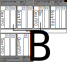
\includegraphics[width=\columnwidth]{\chapterdirectory/figure/dual_store/f07.pdf}
\caption{%
The data message moves from one core's outgoing data queue to the other's
incoming one.
}
\end{subfigure} &
\begin{subfigure}[t]{0.47\textwidth}
\includegraphics[width=\columnwidth]{\chapterdirectory/figure/dual_store/f08.pdf}
\caption{%
Upon reception of data, $C_B$ simply completes its core's request.
}
\end{subfigure}
\end{tabular}
\end{center}
\caption{Illustrations for \textbf{Parallel Stores}}
\label{fig:split_msi_dual_store}
\end{figure}
% Very simple example that must be fully illustrated to show how the FIFOs work.
\stopallthesefloats

\stopallthesefloats{}
\newpage{}
\section{Variants}
This section presents the most common variants of the MSI. In effect, the main
factor of a cache coherence protocol's efficiency is how frequently it needs to
fetch or write data to the main memory. As a result, it is unsurprising to see
that all of these optimizations are focused on removing that necessity in
certain common scenarios. Each of them adds a new stable state, corresponding
to a new permission or new responsibility, and each one can be combined with
the others to form a new variant (forming for example, the MESI, MOESI, and
MESIF protocols).

\paragraph{Exclusive State}
The Exclusive state (\texttt{E}) is equivalent to the \texttt{S} state, with the
added information that no other cache currently holds any copy of the memory
element. As a result, the cache modifying the value of its copy of the memory
element without broadcasting for new permission does not violate
Properties~\ref{prop:system_wide_value} and \ref{prop:swmr}. It does, however,
mean that the coherence manager must be able to detect that no caches hold any
copy of the memory element, which implies some change in how caches evict
from the \texttt{S} state, as they otherwise need not do inform any other
component.

\paragraph{Owned State}
The Owned state (\texttt{O}) allows a cache to keep its modified copy of a
memory element without having to perform a write-back when another cache asks
for a read-only copy of that memory element.

\paragraph{Forward State}
The Forward state (\texttt{F}) is equivalent to an \texttt{S} state where the
cache is also in charge of providing a copy of the memory element to any cache
that demand it.

\stopallthesefloats{}
\section{Cache Line Organization}
Caches hold a finite amount of cache lines. Thus, at some point, the need for a
new cache line when none are available may arise. Deciding which cache line to
evict in order to store the new one has a very important impact on performance.
This is typically decided by two factors: its placement policy and its
replacement policy. These two policies interact: the placement policy determines
which group of cache lines are considered by the replacement policy.

\subsection{Replacement Policies}
The cache eviction policy is the algorithm used to determine which line to
evict when there is no more room. The optimal strategy would ensure that the
line that is evicted is the one that would not be used for the longest time.
However, being able to determine which line this is would require explicit
management of the caches.

Since it is commonly assumed that data recently accessed is likely to be
accessed again soon (a principle known as \textit{locality of reference}), the
most common replacement strategy is to choose the least recently used cache
line as the one to evict. This is referred to as the \textit{LRU} policy.
However, keeping accurate track of which line was accessed last is costly in
both space and time, and so, in practice, a less precise approach, the
Pseudo-LRU (or \textit{PLRU}) is implemented instead. The principle behind
\textit{PLRU} is similar to having a binary tree, with the leaves corresponding
to cache lines. Each node of the tree has a single bit. This bit indicates which
of the two children to follow to find a cache line that was not recently used.
When using any of the cache lines, all nodes in the path leading to it are set
so that they point to a node not also in the path.

Other replacement policies include \textit{FIFO}, in which the cache line that
was the least recently \textit{allocated} is evicted, and cache line uses have
no impact; using frequency of use instead of date, in something similar to the
LRU policy (called \textit{LFU}, for Least-Frequently Used); and random
replacement (\textit{RR}).

These policies are applied to a set of cache lines. Exactly what lines are part
of this set is determined by the placement policy.

\begin{figure}[hbt!]
\begin{center}

\begin{tikzpicture}[->,>=stealth',shorten >=1pt,auto,  semithick]
\tikzstyle{address} = [state,rectangle,  node distance = 0.5cm and 2cm]
\tikzstyle{cacheline} = [state,rectangle, node distance = 0.5cm and 2cm]

\node[cacheline] (CL0) {Cache Line 0: A [3]};
\node[cacheline] (CL1) [below = of CL0] {Cache Line 1: B [2]};
\node[cacheline] (CL2) [below = of CL1] {Cache Line 2: C [1]};
\node[cacheline] (CL3) [below = of CL2] {Cache Line 3: D [0]};

\node[] (sep0) [right = of CL1,xshift=-1em,yshift=-2em] {$ \Longrightarrow $};

\node[cacheline] (CL0b) [right = of CL0] {Cache Line 0: E [0]};
\node[cacheline] (CL1b) [below = of CL0b] {Cache Line 1: B [3]};
\node[cacheline] (CL2b) [below = of CL1b] {Cache Line 2: C [2]};
\node[cacheline] (CL3c) [below = of CL2b] {Cache Line 3: D [1]};

\node[] (sep1) [right = of CL1b,xshift=-1em,yshift=-2em] {$ \Longrightarrow $};

\node[cacheline] (CL0c) [right = of CL0b] {Cache Line 0: E [1]};
\node[cacheline] (CL1c) [below = of CL0c] {Cache Line 1: B [3]};
\node[cacheline] (CL2c) [below = of CL1c] {Cache Line 2: C [0]};
\node[cacheline] (CL3c) [below = of CL2c] {Cache Line 3: D [2]};
\end{tikzpicture}

\end{center}
\caption{Example of LRU Replacement Policy}
\label{fig:replacement:lru}
\end{figure}

Figure~\ref{fig:replacement:lru} is an example of LRU replacement
policy in action: in a cache of four lines, the memory elements $A$, $B$, $C$,
and $D$ were initially loaded, in that order. In the figure, the rightmost
number in each cache line indicates its index for the LRU replacement policy.
The figure shows what happens when a memory element $E$ is loaded, then the
memory element $C$ is accessed. Because $A$ was the least-recently used element,
it is the one that was evicted upon insertion of $E$. As it was just added, the
element $E$ is considered as having been accessed, and all other indices are
updated accordingly. The figure then shows what happens when $C$ is loaded: all
indices strictly below $C$'s are increased by one, then the index of $C$ is set
to $0$, marking it as the most recently used cache line.

\subsection{Placement Policies}
\begin{figure}[hbt!]
\begin{center}

\begin{tikzpicture}[->,>=stealth',shorten >=1pt,auto,  semithick]
\tikzstyle{address} = [state,rectangle,  node distance = 0.5cm and 3cm]
\tikzstyle{cacheline} = [state,rectangle, node distance = 0.5cm and 3cm]

\node[address] (ADDR0)        {Address 0};
\foreach \c in {1,...,7}
{
   \node[address] (ADDR\c)  [below = of ADDR\the\numexpr \c - 1\relax]    {Address \c};
}

\node[cacheline] (CL0) [right = of ADDR0] {Cache Line 0};
\foreach \c in {1,...,7}
{
   \node[cacheline] (CL\c)  [below = of CL\the\numexpr \c - 1\relax]    {Cache Line \c};
}

\node[address] (ADDR8) [right = of CL0] {Address 8};
\foreach \c in {9,...,15}
{
   \node[address] (ADDR\c)  [below = of ADDR\the\numexpr \c - 1\relax]    {Address \c};
}

\foreach \cc in {0,...,7}
{
   \foreach \cl in {0,...,7}
   {
      \path (ADDR\cc.east) edge (CL\cl.west);
   }
}
\foreach \cc in {8,...,15}
{
   \foreach \cl in {0,...,7}
   {
      \path (ADDR\cc.west) edge (CL\cl.east);
   }
}

\end{tikzpicture}

\end{center}
\caption{Example of Fully Associative Cache Organization}
\label{fig:placement:fully_associative}
\end{figure}

\begin{figure}[hbt!]
\begin{center}
\input{\chapterdirectory/figure/cache_placement_direct_map.tex}
\end{center}
\caption{Example of Directly Mapped Cache Organization}
\label{fig:placement:direct_map}
\end{figure}

\begin{figure}[hbt!]
\begin{center}
\input{\chapterdirectory/figure/cache_placement_set_associative.tex}
\end{center}
\caption{Example of Set Associative Cache Organization}
\label{fig:placement:set_associative}
\end{figure}

Placement policies determine where a memory element can be stored within the
cache, according to the memory element's address. There are three common
strategies: allow it to go anywhere; allow it to go only at one location; and
allow it to go anywhere within a group of cache lines;

A cache in which memory elements can be placed anywhere is called a
\textit{fully associative} cache. This makes the replacement policy able to
perform at its best, since it applies to the whole cache at once. However,
locating a cache line is costly, since it can effectively be anywhere in the
cache. An example of fully associative cache organization is shown in
Figure~\ref{fig:placement:fully_associative}.

A cache in which each address maps to a single cache line is called a
\textit{direct-mapped} cache. This effectively negates the need for a
replacement policy. Access to a cache line is very fast. Depending on
the mapping algorithm and the accesses made, this can end up being very
efficient. However, even a very frequently accessed memory element is at risk of
being evicted if another memory element that maps to same cache line is also
accessed. Furthermore, this may lead to cache lines being evicted even when
other cache lines remain unused. An example of directly mapped cache
organization is shown in Figure~\ref{fig:placement:direct_map}.

A cache in which a mix of both strategies is used is called a
\textit{set-associative} cache. This is equivalent to having the cache be split
into equally sized groups of cache lines, and applying the direct mapping to
groups instead of single cache lines: each address is mapped to a group, but the
memory element can end up anywhere within that group. The replacement policy is
then only applied within the relevant group, which is much cheaper than a
cache-wide implementation. Additionally, more frequently used memory elements
sharing a set with other memory elements are less likely to get evicted. The
issue of cache lines being evicted despite having potentially unused cache lines
is still there, but only if these unused cache lines are not part of the group
to which the newly allocated cache line belongs. An example of set associative
cache organization where each set has two lines is shown in
Figure~\ref{fig:placement:set_associative}.

\stopallthesefloats{}
\section{Conclusion}
This chapter has shown how UPPAAL's model checking capabilities can be exploited
to analyze the interference caused by cache coherence on the model from
Chapter~\ref{cha:modeling_cache_coherence}.

This analysis starts by a computation of the WCET for each program. Useful in
itself, this analysis is extended by that of the WCET for these programs with
the architecture in different configurations in order to extract more
information about how much of the execution time is caused by interference.

In order to more precisely understand what determine the WCET and to provide
the user with information about elements of the program that can directly be
manipulated, the analysis proceeds by an categorization of the accuracy of each
instruction. This indicates which instructions are unaffected by the
interference, which instructions are always time-consuming, and which
instructions take a varying amount of time depending on the execution. By
looking at the accuracy of all accesses made on each memory element, patterns
for these instructions of varying execution time can sometimes be found, which
results in a more predictable system.

The determining factor for the accuracy of instructions is then properly
defined. This corresponds to a categorization of all external queries depending
on their effects on the permissions held by a cache, and whether a loss of
permission led to an instruction taking additional time. Thus, three categories
of interference are defined: minor (no change of permission, but loss of time
due to query processing), demoting (loss of writing permission), and expelling
(loss of all permissions).

Finally, analyses are performed in order to determine how each instruction
interfere with the other instructions. This results in a graph showing, for
each instruction, which instruction can generate interference that will
directly impact it, the category of this interference, and whether this
interference occurs on all possible executions or not.

This provides the user with a clear understanding of the causes and effects of
cache coherence interference on the programs' instructions, opening the way to
finding means of mitigation for this interference.

\stopallthesefloats{}

   \chapter{Objective}
\label{cha:second_intro}
\definechapterdirectory{src/second_intro}

The introduction of multi-core processors in critical avionic systems requires
the ability to sufficiently predict their behavior so that certification of the
system is achievable. Indeed, the parallel nature of multi-core processors
leads to numerous interactions that do not strictly pertain to the objective
of the applications being ran. This large amount of unprompted interactions
render execution times difficult to predict and subject to large variations.
Among the main causes of large time variations is cache coherence, the
mechanism ensuring that data modifications performed by programs running in
parallel are properly propagated. While cache coherence can be implemented with
predictability in mind (see
Section~\ref{sec:rel_work:handling_it:through_hardware}), this requires hardware
modifications, precluding such solutions in an aeronautical context.
Unfortunately, the available strategies to predict worst-case execution time of
applications running on multi-core \textit{Commercial Off-The-Shelf} processors
require cache coherence to be deactivated (see
Section~\ref{sec:rel_work:handling_it:accepting_it} and
Chapter~\ref{cha:analyzing_rel_work}).

This thesis proposes solutions to begin addressing the issue of cache coherence
predictability in an aeronautical context. To do so, it provides the applicant
with tools that can expose and explain the interference generated by cache
coherence. In this chapter is provided a summary, the limitations, and
suggestions of future improvements for each contribution made in this thesis.

\subsection{Hypotheses and Limitations}
\label{sec:thesis_hypotheses}
This section presents the hypotheses made on the context in order to limit the
scope of this thesis, as well as the reason behind these limitations and, when
applicable, how these could be removed in future works.

The first scope restrictions stem from the aeronautical context. Indeed:
\begin{itemize}
\item Only COTS architectures are considered. The use of self-made hardware is
not deemed acceptable in critical systems such as avionics.
\item Uses cache coherence. Using multi-core processors without cache coherence
prevents any gain they would otherwise provide over single-core processors when
running application with parallel processing.
\item Snooping-based cache coherence. This is the more common approach to cache
coherence in COTS, and thus makes for a good starting point. Extending this
thesis to also handle directory-based cache coherence would require the creation
of a different architecture model.
\end{itemize}

Other restrictions are more related to what the thesis' time constraints
permitted. The focus stayed on cache coherence itself, since this is what the
existing literature consistently avoids. Thus, elements that are already
explored in other numerous works have not been expended upon past the bare
minimum. An example of architecture complying with these restrictions can
be seen in Figure~\ref{fig:second_intro:typical_arch}.

\begin{figure}[hbt!]
\begin{center}
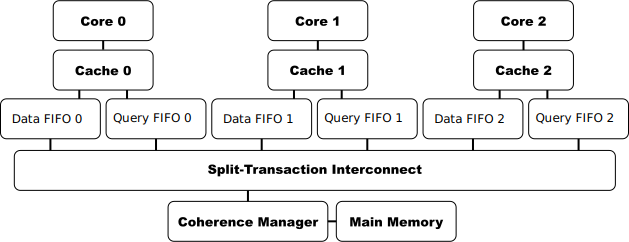
\includegraphics[width=\textwidth]{\chapterdirectory/figure/typical_arch3.pdf}
\end{center}
\caption{Typical profile of the targeted architecture}
\label{fig:second_intro:typical_arch}
\end{figure}

\begin{itemize}
\item No cache hierarchy. The coherence is studied within a single level of
cache, there is no issue of memory element propagation across L1, L2, or L3
caches. Adding proper support for cache hierarchy to the tools presented in this
thesis would require a large number of modifications.
\item One core per cache. The solution proposed in this thesis does not properly
handle multiple cores per cache, as the model fails to account for the
originator of each request in at least one of its functionalities. Unless as of
yet unknown issues arise, this limitation should be fairly easily removed.
\item Fully associative cache placement policy. Supporting the segregation of
cache lines would add a layer of complexity without being a fundamental change
in what the tools prove to be possible. Allowing configuration by the user so
that other placement policies may be used should be straight forward, and is
only absent because of its low priority.
\item LRU cache replacement policy. While a replacement policy had to be chosen,
the most popular one, PLRU, was not the one implemented. LRU is easier to
debug, which is why it was chosen. Here also, adding support for other policies
would not constitute a major change in the model, but neither was it considered
a high priority feature.
\item Simplified program representation. The focus is really put on cache
coherence. No matter how complex, programs only interact with cache coherence
through memory accesses. Thus, only sequences of memory accesses are represented
and, by default, instruction jumping and branching is not supported.
Technically, this can already be bypassed by creating a new automaton for each
of the more complex program, however, automation of the automaton creation is
required before such a solution can be considered reasonable.
\end{itemize}

Lastly, the tools proposed in this thesis only constitute part of the solution
needed to properly analyse multi-core processors for use in avionics:
\begin{itemize}
\item Results focused on cache coherence only. For accurate measurement of the
effects of interference on applications running in a multi-core, the separate
analysis of sources of interference is inadequate as not only are these sources
not independent, but the effects of each source interference can, by definition,
alter the behavior of the application and thus lead to the other sources of
interference having a different effect on the application. Assuming a worst case
for each source of interference does not ensure that the global worst case is
measured (a principle known as \textit{timing anomaly}). Thus, the contributions
made in this thesis would need to be integrated into an all-encompassing
framework in order to allow adequate estimation of the WCET.
\end{itemize}

\subsection{Framework Overview}
\label{sec:second_intro:framework}
Figure~\ref{fig:second_intro:approach} presents the general framework proposed
in this thesis for the analysis of the impact of cache coherence on software
running on a multi-core COTS system.

Given an architecture, the applicant performs an identification of the cache
coherence mechanisms. This removes any ambiguities that may be lingering in the
description of the cache coherence protocol from the architecture's
documentation. This process is described in
Chapter~\ref{cha:identifying_cache_coherence} and involves the use of
performance monitors in order to observe the behavior of the architecture's
cache coherence mechanisms and compare it with that of a hypothetical cache
coherence protocol. If the two match, the applicant thus obtains an
ambiguity-free cache coherence protocol description for the architecture.

Using this ambiguity-free cache coherence protocol, the temporal cost of each
operation is quantified through benchmarks. Indeed, now that all relevant
coherence states and behaviors are known, the applicant can be sure their
measures are not missing important results. This step is not expanded upon by
the thesis, as the existing literature already covers it (see
Chapter~\ref{cha:micro-benchs}). With these measures, a profile of the
architecture's cache coherence mechanisms has been obtained.

To evaluate the impact of cache coherence on the execution of software, this
thesis proposes the use of formal methods. This requires the creation of a model
for the architecture (see Chapter~\ref{cha:modeling_cache_coherence}), as well
as the definition of the appropriate queries in order to retrieve information
that can be used by the applicant through model checking (see
Chapter~\ref{chap:exposing_interference}).

\begin{figure}[hbt!]
\iffalse
\begin{subfigure}[t]{\textwidth}
\centering
\begin{tikzpicture}[
  font=\sffamily,
  every matrix/.style={ampersand replacement=\&,column sep=2.5cm,row sep=1cm},
  source/.style={draw,thick,rounded corners,fill=yellow!20,inner sep=.3cm},
  process/.style={draw,thick,circle,fill=blue!20},
  sink/.style={source,fill=green!20},
  datastore/.style={draw,very thick,shape=datastore,inner sep=.3cm},
  dots/.style={gray,scale=2},
  to/.style={->,>=stealth',shorten >=1pt,semithick,font=\sffamily\footnotesize},
  every node/.style={align=center}]

  % Position the nodes using a matrix layout
  \matrix{
    \node[datastore] (architecture) {Architecture};
      \& \node[sink] (identification) {%
         \begin{tabular}{@{}c@{}}
            Cache Coherence Identification\\
            (Section~\ref{fr:sec:identify})
         \end{tabular}
         };
      \&
    \node[datastore] (cacheprotocol) {%
         \begin{tabular}{@{}c@{}}
            Cache Coherence\\ Protocol
         \end{tabular}
         };
      \\
  };

  % Draw the arrows between the nodes and label them.
  \draw[to] (architecture) to (identification);

  \draw[to] (identification) to (cacheprotocol);
\end{tikzpicture}

\end{subfigure}
\begin{subfigure}[t]{\textwidth}
\vspace{2em}
\centering
\begin{tikzpicture}[
  font=\sffamily,
  every matrix/.style={ampersand replacement=\&,column sep=2.5cm,row sep=1cm},
  source/.style={draw,thick,rounded corners,fill=yellow!20,inner sep=.3cm},
  process/.style={draw,thick,circle,fill=blue!20},
  sink/.style={source,fill=green!20},
  datastore/.style={draw,very thick,shape=datastore,inner sep=.3cm},
  dots/.style={gray,scale=2},
  to/.style={->,>=stealth',shorten >=1pt,semithick,font=\sffamily\footnotesize},
  every node/.style={align=center}]

  % Position the nodes using a matrix layout
  \matrix{
   \&
    \node[datastore] (cacheprotocol) {%
         \begin{tabular}{@{}c@{}}
            Cache Coherence\\ Protocol
         \end{tabular}
         };
      \&
   \\
    \node[datastore] (architecture) {Architecture};
      \&
      \node[source] (benchmarking) {%
         \begin{tabular}{@{}c@{}}
            Benchmarking\\
            (Section~\ref{fr:sec:benchs})
         \end{tabular}
      };
      \&
    \node[datastore] (cacheperformance) {%
         \begin{tabular}{@{}c@{}}
            Cache Coherence\\
            Performance
         \end{tabular}
      };
      \\
  };

  % Draw the arrows between the nodes and label them.
  \draw[to] (architecture) to (benchmarking);
  \draw[to] (cacheprotocol) to (benchmarking);

  \draw[to] (benchmarking) to (cacheperformance);
\end{tikzpicture}

\end{subfigure}
\begin{subfigure}[t]{\textwidth}
\vspace{4em}
\centering
\input{\chapterdirectory/figure/approach_step3.tex}
\end{subfigure}
\fi
\centering
\begin{tikzpicture}[
  font=\sffamily,
  every matrix/.style={ampersand replacement=\&,column sep=2.5cm,row sep=1cm},
  source/.style={draw,thick,rounded corners,fill=yellow!20,inner sep=.3cm},
  process/.style={draw,thick,circle,fill=blue!20},
  sink/.style={source,fill=green!20},
  datastore/.style={draw,very thick,shape=datastore,inner sep=.3cm},
  dots/.style={gray,scale=2},
  to/.style={->,>=stealth',shorten >=1pt,semithick,font=\sffamily\footnotesize},
  every node/.style={align=center}]

  % Position the nodes using a matrix layout
  \matrix{
    \node[datastore] (architecture) {Architecture};
      \& \node[sink] (identification) {%
         \begin{tabular}{@{}c@{}}
            Cache Coherence Identification\\
            (Chapter~\ref{cha:identifying_cache_coherence})
         \end{tabular}
         };
      \&
    \node[datastore] (cacheprotocol) {%
         \begin{tabular}{@{}c@{}}
            Cache Coherence\\ Protocol
         \end{tabular}
         };
      \\


   \&
      \&
   \\
      \&
      \node[source] (benchmarking) {%
         \begin{tabular}{@{}c@{}}
            Benchmarking\\
            (Chapter~\ref{cha:micro-benchs})
         \end{tabular}
      };
      \&
    \node[datastore] (cacheperformance) {%
         \begin{tabular}{@{}c@{}}
            Cache Coherence\\
            Performance
         \end{tabular}
      };
      \\



   \&
      \&
   \\
      \node[datastore] (application) {Application};
      \&
      \node[sink] (uppaal) {
         \begin{tabular}{@{}c@{}}
            UPPAAL Analysis\\
            (Chapters~\ref{cha:modeling_cache_coherence} and
            \ref{chap:exposing_interference})
         \end{tabular}
         };
      \&
      \node[datastore] (coherenceeffect) {%
         \begin{tabular}{@{}c@{}}
            Cache Coherence\\
            Impact
         \end{tabular}
      };
   \\
  };

  % Draw the arrows between the nodes and label them.
  \draw[to] (architecture) to (identification);

  \draw[to] (identification) to (cacheprotocol);



  \draw[to] (architecture) to (benchmarking.north west);
  \draw[to] (cacheprotocol) to (benchmarking.north east);

  \draw[to] (benchmarking) to (cacheperformance);



  \draw[to] (architecture) to (uppaal.north west);
  \draw[to] (cacheperformance) to (uppaal.north east);
  \draw[to] (cacheprotocol) to (uppaal);
  \draw[to] (application) to (uppaal);

  \draw[to] (uppaal) to (coherenceeffect);
\end{tikzpicture}

\caption{Approach Overview}
\label{fig:second_intro:approach}
\end{figure}


\stopallthesefloats
\section{Conclusion}
This chapter concludes the context part of the thesis by clearly defining the
objective of this thesis and curtailing its target application.

The next part of the thesis presents a selection of the existing literature
relevant to this thesis. It starts with a chapter focused on benchmarking
(Chapter~\ref{cha:micro-benchs}), providing a description of approaches that can
be used to measure the performance of the architecture's cache coherence
mechanisms once the protocol has been identified.

Literature around the broader issue of using a multi-core processor's caches in
a critical real-time environment is then presented
(Chapter~\ref{cha:handling_it}). None of the existing solutions allow the use of
cache coherence within an aeronautical context, but there are ways to still
benefit from caches by adhering to restrictions on their use.

Lastly, the related works part of this thesis features a chapter on approaches
similar to that presented in this thesis for the use of formal methods to
analyze an architecture (Chapter~\ref{cha:analyzing_rel_work}). It shows that
the use of timed automata eases the creation of both readable and modular
models.


   \part{Related Works}
   \definechapterdirectory{src/related_works}
\chapter{Micro-Stressing Benchmarks}
\label{cha:micro-benchs}
This chapter presents strategies relying on benchmarks to figure out the
characteristics of an architecture, be it its speed, the capacity of its
components, or other information not sufficiently detailed in the architecture's
documentation. Having properly characterized the architecture is a
necessary preliminary step to the analysis of interference. Indeed, to
understand the effects the interference has on running software, a
quantification of the architecture's components capabilities is necessary, as
determining which parallel accesses would interfere with one another is
otherwise impossible.

In the contributions made by this thesis, the objective of the benchmarks is not
only to measure the maximum performance of the cache coherence mechanisms, but
also ascertain that they are fully understood by the user. This is a vital part
of the characterization process, and solutions for mechanisms much simpler than
cache coherence have already been explored. For example, the first section of
this chapter showcases two papers proposing solutions to detect hidden
correlations between components.

Once the mechanisms have been understood, then the performance measurements can
proceed, as the user is now fully aware of what is being measured. The second
section of this chapter is thus about papers on the use of benchmarks for the
performance analysis of cache coherence.

Lastly, this chapter presents a paper on the use of benchmarks to remedy a lack
of performance monitors. Such an approach could be used to implement the
solution proposed in Chapter~\ref{cha:identifying_cache_coherence} if the user
cannot find the appropriate performance monitors.

Because the terms are recurrently used thorough this chapter, definitions for
\textit{execution time}, \textit{overhead}, and \textit{bandwidth} are provided below.

\begin{definition}[Configuration]
\label{def:configuration}
A configuration is defined as the combination of the mapping of programs on each
core, the hardware's settings, and the initial state of the architecture prior
to program execution.
\end{definition}

\begin{example}[Configuration]
\label{ex:configuration}
Running a sequence of instructions in isolation, and running that same sequence
of instructions while other programs are running on other cores correspond to
two separate configurations.
\end{example}

\begin{definition}[Execution Time]
The execution time of a list of instructions on a certain configuration is the
time between the emission of the first of the instructions and the last
instruction of the list being seen as completed by the emitter.
\end{definition}

\begin{example}[Execution Time]
In the case of two successive loads, the execution time corresponds to the time
elapsed between core emitting the first load instruction to its cache, and the
cache providing the data for the second load instruction.
\end{example}


\begin{definition}[Overhead]
Given $T_A$ and $T_B$ two execution times of a same list of instructions from
two separate arbitrary configurations $A$ and $B$, such that $T_B \ge T_A$, The
overhead $O$ of being in configuration $B$ over configuration $A$ is defined as:
\[ O = T_B - T_A \]
\end{definition}

\begin{example}[Overhead]
If the two configurations of Example~\ref{ex:configuration} yielded an execution
time of 5 CPU cycles and 13 CPU cycles respectively, the overhead incurred
because of the other programs running in parallel would be $13 - 5 = 8$ CPU
cycles.
\end{example}

\begin{definition}[Bandwidth]
Bandwidth is the amount of data (e.g.~bits, bytes, words) that can be
transferred from one component to another within a given time frame.
\end{definition}

\begin{example}[Bandwidth]
A CPU attempting to write a sequence of data with a size of 512MB in the memory
would have to pass the information through all the mechanisms between itself and
the memory. The amount of data that went through all the mechanisms within
either a CPU cycle or a microsecond is considered to be the bandwidth.
\end{example}

\stopallthesefloats{}
\section{Detecting Component Correlation}
\stopallthesefloats{}
\stopallthesefloats
\subsection{Evaluating Interference Through Resource-Stressing}
\label{sec:radojkovic}
\cite{10.1145/2086696.2086713} presents a strategy to characterize the
sensibility of a shared resource to temporal interference. The general idea
behind the approach is to perform a stressing benchmark on an architecture's
resource with only that single thread running (i.e.~running in isolation), and
compare the result with the same test in which multiple threads of the stressing
benchmark run in parallel, in a metric called \textit{slowdown factor} (see
Definition~\ref{def:slowdown-factor}).

\begin{definition}[Slowdown Factor]
\label{def:slowdown-factor}
Given a benchmark targeting a specific component, its application using a single
thread in isolation resulting in a execution time $n$, and its application while other
threads are stressing components (potentially the same one) yielding a execution time
of $m$, the slowdown factor $f$ is defined as:
\[f = \frac{n}{m}\]
\end{definition}

This slowdown factor indicates how sensible the component targeted by the
measured benchmark is to interference, and thus how large the execution time
variations caused by parallel access to that component will be. By having the
other threads target different components, correlation between them can be
exposed: if the slowdown factor is higher than $1.0$, some interactions occur
between these components, and the other components are able to generate
interference on any application using the component targeted by the measured
thread.
\begin{figure}[hbt!]
\begin{center}
%\lstinputlisting{\chapterdirectory/figure/micro_bench/atom_bench.txt}
\begin{tabular}{r|l|l}
\hline
Line  & Source code                    & Explanation\\
\hline
001   & {\lstinline!movl %1, %ecx!}    & initialize loop counter \textit{ecx}
({\lstinline!%1!} is an input parameter)\\
002   & {\lstinline!label_intAdd:!}    & beginning of the loop\\
003   & {\lstinline!add %eax, %ebx!}   & target instruction\\
004   & {\lstinline!add %ebx, %eax!}   & target instruction\\
...   & {\lstinline!...!}              & ...\\
...   & {\lstinline!...!}              & ...\\
252   & {\lstinline!add %ebx, %eax!}   & target instruction\\
253   & {\lstinline!decl %ecx!}        & decrement loop counter\\
254   & {\lstinline!cmp %ecx, $0!}     & compare loop counter with 0\\
255   & {\lstinline!jne label_intAdd!} & if (counter != 0) jump to the beginning of the loop\\
\hline
\end{tabular}
\end{center}
\caption{\textit{intAdd} Benchmarking Code (taken from
\cite{10.1145/2086696.2086713})}%
\label{fig:micro_bench:atom_bench}
\end{figure}

\begin{figure}[hbt!]
\begin{center}
\lstinputlisting{\chapterdirectory/figure/micro_bench/atom_init.txt}
\end{center}
\caption{Memory Benchmark Initialization Code (taken from
\cite{10.1145/2086696.2086713})}%
\label{fig:micro_bench:atom_init}
\end{figure}

The benchmarks of \cite{10.1145/2086696.2086713} are implemented following the
pattern shown in Figure~\ref{fig:micro_bench:atom_bench}: a simple loop applying
the appropriate instruction numerous times. For memory access benchmarking, a
slightly different strategy is used (see
Figure~\ref{fig:micro_bench:atom_init}): each loaded memory element contains the
address of the next memory element to load, a principle known as pointer
chasing.

\begin{figure}[hbt!]
\begin{center}
\includegraphics[width=\textwidth]{\chapterdirectory/figure/micro_bench/atom_stress.pdf}
\end{center}
\caption{Slowdown factor on the Intel Atom Z530 (taken from \cite{10.1145/2086696.2086713})}%
\label{fig:micro_bench:atom_stress}
\end{figure}

Figure~\ref{fig:micro_bench:atom_stress} shows the approach of
\cite{10.1145/2086696.2086713} working at its best. This is the result on an
Intel Atom Z530, which features a single core capable of running two parallel
threads. The lines correspond to the benchmark being measured, the columns
correspond to the target of the benchmark being used as a source of
interference.

\begin{figure}[hbt!]
\begin{center}
\includegraphics[width=0.6\textwidth]{\chapterdirectory/figure/micro_bench/core2quad.png}
\end{center}
\caption{The Intel Core2Quad architecture (taken
from \cite{10.1145/2086696.2086713})}%
\label{fig:micro_bench:core2quad}
\end{figure}

\begin{figure}[hbt!]
\begin{center}
\includegraphics[width=\textwidth]{\chapterdirectory/figure/micro_bench/shared_cache_interference_detect.png}
\end{center}
\caption{Slowdown factor on the Intel Core2Quad within the same cluster (taken
from \cite{10.1145/2086696.2086713})}%
\label{fig:micro_bench:core2quad_stress}
\end{figure}

The application on a multi-core processor, however, is not as informative:
Figure~\ref{fig:micro_bench:core2quad_stress} shows the same experiment
performed within a cluster of an Intel Core2Quad (two separate cores that share
the same L2 cache, see Figure~\ref{fig:micro_bench:core2quad}). The results
indicate no unexpected slowdowns from the simultaneous use of components.
Information on slowdown due to simultaneous use of caches points is still
relevant and points to running two parallel cache intensive programs being
slower than one after the other.

\begin{figure}[hbt!]
\begin{center}
\includegraphics[width=0.5\textwidth]{\chapterdirectory/figure/micro_bench/simultaneous_stressing.png}
\end{center}
\caption{Standard benchmark interference on the Intel Core2Quad (taken
from \cite{10.1145/2086696.2086713})}%
\label{fig:micro_bench:core2quad_max_interference}
\end{figure}

\cite{10.1145/2086696.2086713} does not provide the analysis of potential
interference channels with more than two components in use simultaneously, but
it does analyze the slowdown factor suffered by some standard benchmark
applications running on one core when other components are being stressed by all
the other core.
The results are shown in
Figure~\ref{fig:micro_bench:core2quad_max_interference}. The observed slowdown
factors are very small, regardless of the components being stressed by the other
cores. This points to the use of standard benchmarks being poor indicators of
the worst slowdown that can be suffered because of interference. Indeed, none of
these results reflect the high slowdown factor that was obtained when even just
two cores stressed the same L2 cache. Thus, the effects of interference on an
application that uses the L2 cache more than those standard benchmarks is likely
to be much higher than what the results from
Figure~\ref{fig:micro_bench:core2quad_max_interference} would lead to believe.

\iffalse % Let's ignore the paper's actual contribution, shall we?
Figure~\ref{fig:micro_bench:atom_stress} shows the slowdown factors obtained by
this strategy on a Intel Atom Z530, which features a single core capable of
running two parallel threads. The lines correspond to the benchmark being
measured, the columns correspond to the target of the benchmark being used as
a source of interference.

The paper presents the same table for two other architectures: an Intel Pentium
D, with two cores each capable of a single thread; and an Intel Core2Quad
Q9550, with four cores, also only capable of a single thread. The resulting
slowdown factors for this particular set of shared resources for these two
architectures is considerably less impressive however, as only at most
two of these resources are actually shared by the separate cores (\textit{L2
cache}, and main memory access - \textit{mem\_bw}). Nevertheless, performing
such measurements does confirm that the resources are indeed not shared and
thus unable to interfere with one another, and the results do point out
L2 cache accesses to be a bottleneck on the Core2Quad architecture, with a
slowdown factor of $14.4$.

The results shown in \cite{10.1145/2086696.2086713}, especially those in
Figure~\ref{fig:micro_bench:atom_stress}, do make a strong argument against the
use of simultaneous multi-threading on a single core in applications with
real-time constraints, as having to taking into account the slowdown factor of
each of these shared resources makes the estimation of a precise worst-case
execution time that much more difficult. Unsurprisingly, such results are the
reason for simultaneous multi-threading being forbidden in aeronautical
contexts.
\fi

To summarize, the strategy employed here forms the basis of covert interference
channel identification, as it exposes potentially unknown links between
components, but it also provides some quantification of the architecture's
capabilities through the slowdown factor, and argues for the use of
micro-stressing benchmarks over that of standard ones for a true observation of
the maximum impact of interference, including for interference related to the
use of caches.

The next paper expands on this approach, by using performance monitors to
measure more than cycle counts, and thus learn more about how components
interact.

\stopallthesefloats

\stopallthesefloats{}
\subsection{Architecture and Application Characterization}
\begin{figure}
\begin{center}
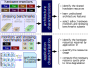
\includegraphics[width=0.7\textwidth]{\chapterdirectory/figure/micro_bench/co_running_apps_cots.pdf}
\end{center}
\caption{Strategy overview for \cite{Bin14} (Figure taken from the paper)}%
\label{fig:micro_bench:co_running_apps_cots}
\end{figure}

The approach presented in \cite{Bin14} can be seen as a follow up to the one of
\cite{10.1145/2086696.2086713}: the correlations between components that were
exposed are used to tailor the benchmarks performed on the application.  The
process is summarized in Figure~\ref{fig:micro_bench:co_running_apps_cots}.

When profiling the architecture, the objective is to characterize the hardware
itself, in order to identify shared hardware resources (including some that may
be missing from the architecture's documentation), determine their behavior when
in contention, potentially uncover unsuspected interactions between hardware
components, measure pertinent execution times and maximum bandwidths. To do so, the
approach starts with a comparison of each benchmark running in isolation and
running with other copies of itself running in parallel, as in the approach from
Section~\ref{sec:radojkovic} (the top-left diagonal in
Figure~\ref{fig:micro_bench:atom_stress}). In a second step, benchmarks
targeting different features are launched together. This provides information on
which parallel resource accesses affect one another. Here also, the approach is
similar to the one in Section~\ref{sec:radojkovic} (all cases other than the
top-left diagonal in Figure~\ref{fig:micro_bench:atom_stress}). Note that this
similarity with the previous section is to be expected, as both approaches make
similar assumptions on the availability of standard monitoring resources.  The
main difference being the use of hardware monitors other than the cycle counter
in \cite{Bin14}, where performance counters such as ``number of L1 hits'' are
also used in order to obtain a clearer understanding of the architecture, and
thus of the causes of the interference instead of just observing its effects.
This can be used to uncover relations between components despite not having
measured a change of slowdown factor upon their concurrent benchmarking.

Hardware monitors are counters that can be set to increase on the occurrence of
a given event, such as an access to the interconnect, a cache miss, a cache
eviction, and many other. The architecture's documentation generally provides a
list of events that can be monitored. These monitors can be reset, temporarily
frozen, or set to track another type of event during the execution of programs,
making them a very useful debugging and analysis tool.

\cite{Bin14} proposes using this information to limit the analysis made on
programs to what is truly necessary. Indeed, the architecture characterization
phase having already determined which combinations of benchmarks are redundant
for the analysis of interference between tasks, only a subset needs to be
employed to fully understand the impact of resource sharing on the
timing of the applications.

This subset of benchmark combinations is then used to analyze how much usage of
a particular resource is needed before an application slows down. In effect,
this indicates the minimal share of each resource needed for an application to
not suffer drastic worst case execution time slowdowns, and thus helps effective
scheduling of applications on a multi-core processor.

\begin{figure}[hbt!]
\begin{tabular}{cc}
\begin{subfigure}[t]{0.37\textwidth}
\lstinputlisting{\chapterdirectory/figure/micro_bench/paris_thesis_actual_general.txt}
\caption{Performance Counter Management}
\label{fig:micro_bench:co_running_apps_cots_algo_part_one}
\end{subfigure}
&
\begin{subfigure}[t]{0.47\textwidth}
\lstinputlisting{\chapterdirectory/figure/micro_bench/paris_thesis_general.txt}
\caption{Benchmark execution}
\label{fig:micro_bench:co_running_apps_cots_algo_part_deux}
\end{subfigure}
\end{tabular}
\caption{%
Benchmark algorithm used in \cite{Bin14} (extracted from \cite{Bin14Thesis})
}
\label{fig:micro_bench:co_running_apps_cots_algo}
\end{figure}

While \cite{Bin14} does not provide any code extracts, the algorithm can be
found in the associated thesis (\cite{Bin14Thesis}).
Figure~\ref{fig:micro_bench:co_running_apps_cots_algo} shows an overview of
algorithm used by \cite{Bin14}.
Figure~\ref{fig:micro_bench:co_running_apps_cots_algo_part_one} indicates how
the performance monitors are handled. The use of a loop to perform multiple
measures of the same experiment allow capture of the result's variability.
The benchmarked operations take the form shown in
Figure~\ref{fig:micro_bench:co_running_apps_cots_algo_part_deux}: it features an
unrolled loop (with \lstinline!UNROLLED! corresponding to the size of that inner
loop) within another loop, all performing the same operation (writing or
reading). The only reason for there to be an unrolled loop within the primary
loop is to reduce the amount of computations made during the iteration: the
combination of both loops simply makes the operations be performed across
the whole \lstinline!TABLESIZE! addresses. The \lstinline!STRIDE! parameter
corresponds to the gap between accesses, which is there to control the number of
times the same cache line is accessed. \cite{Bin14Thesis} indicates that the
use of the \lstinline!NOP! parameter is there to have idle time between
accesses: it corresponds to a varying number of \lstinline!nop! operations, and
can thus be used to see the effect of temporally spacing out the accesses.

The cache coherence identification part of this thesis
(Chapter~\ref{cha:identifying_cache_coherence}) uses an algorithm similar to the
one shown in Figure~\ref{fig:micro_bench:co_running_apps_cots_algo_part_one} to
observe the behavior of caches. In effect,
Chapter~\ref{cha:identifying_cache_coherence} is a specialized part of the
\textit{learn undisclosed architecture features} section of the
\textit{architecture characterization} process shown in
Figure~\ref{fig:micro_bench:co_running_apps_cots}. Instead of simply detecting
interaction It goes beyond the analysis
of simple interactions to really understand
\stopallthesefloats{}

\stopallthesefloats{}
\section{Analyzing Cache Performance}
The previous section showed approaches to the detection of potential
interference channels that could be applied to any component, but whose
genericity ran the risk of failing to detect complicated relations between
components. This section focuses on approaches that use benchmarks to
characterize cache coherence performance and/or interference channels.
\stopallthesefloats{}
\stopallthesefloats
\subsection{Cost of Cache Coherence}
\cite{Nowotsch2012LeveragingMC} places itself in a context similar to this
thesis: the issues of interference in multi-core architecture preventing their
use in avionics. More precisely, the paper proposes an analysis of an
architecture through benchmarks to ensure that tasks running in parallel can
correctly be time partitioned. The tasks in question involve mixed-criticality,
meaning that some tasks are more important than others, and thus lower
importance tasks must not impede higher importance ones.

The studied architecture is a NXP QorIQ P4080, featuring eight single-thread
cores with their own L1 and L2 caches, and interconnected through a CoreNet
Fabric implementing the MESI cache coherence protocol. There are also two L3
caches accessible through the interconnect.

The main sources of interference studied in \cite{Nowotsch2012LeveragingMC} are
simultaneous accesses to the interconnect and the main memory, as well as the
latencies induced by cache coherence. The idea is to have one core act as the
active observer, meaning that it is where time is measured, but it also performs
some operation. The other cores only act as a source of interference, and
multiple benchmarks are performed to see how increasing the number of secondary
cores influences the time measured by the observer core. This is similar to the
approaches presented in the previous section, with the difference being that
instead of targetting a specific component, the benchmarks are solely focused on
memory access, and the comparison is made on cores performing either
\textit{read} or \textit{write} on memory elements.

For the evaluation of the latencies induced by cache coherence, three categories
of cache coherence benchmarks are considered:
\begin{itemize}
\item \textbf{disabled:} No cache coherence enabled (i.e.~the baseline), where
its mechanisms are disabled and the cores do not target any of the same memory
elements.
\item \textbf{static:} Cache coherence mechanisms are enabled, but the cores
still do not target any of the same memory elements.
\item \textbf{dynamic:} Cache coherence enabled, and cores only target shared
memory elements.
\end{itemize}
This is made possible by the fact that the architecture supports disabling cache
coherence all together. For all three categories, sub-benchmarks are performed,
in which the observer core either reads or writes memory elements while the
secondary core also perform either reading or writing (thus resulting in four
combinations for each category of cache coherence: read read - \textit{rr}, read
- write, \textit{rw}, \textit{wr}, and \textit{ww}).

\begin{figure}[hbt!]
\lstinputlisting{\chapterdirectory/figure/micro_bench/06214768_code.txt}
\caption{%
Algorithm overview for \cite{Nowotsch2012LeveragingMC} (taken from the paper)
}
\label{fig:micro_bench:cache_coherence_avionics_algo}
\end{figure}

Figure~\ref{fig:micro_bench:cache_coherence_avionics_algo} shows the algorithm
used by \cite{10.1109/PACT.2009.22}. Prior to each measurement, the caches are
flushed, then the cores synchronize with each other. Time is recorder using
utilities from the cores, which avoids making \lstinline!time()! be a source of
interference. The measured operation takes three parameters:
\lstinline!OPERATION! corresponds to either reading or writing,
\lstinline!NBYTES! is the number of bytes accessed in a measurement,
\lstinline!GAP! is the distance between the accesses made in order to target
separate cache lines and thus ensure that all accesses are cache misses. The
number of measures is controlled by \lstinline!NMEAS!. The
\lstinline!__asm_write_loop_gap64! corresponds to a \lstinline!meas_loop! for
a writing operation with a gap of 64 bytes.

\begin{figure}[hbt!]
\begin{center}
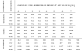
\includegraphics[width=0.7\textwidth]{\chapterdirectory/figure/micro_bench/cache_coherence_avionics.pdf}
\end{center}
\caption{Observed execution times depending on cache coherence and number of
active cores (adapted from \cite{Nowotsch2012LeveragingMC})}%
\label{fig:micro_bench:cache_coherence_avionics}
\end{figure}

The results of these benchmarks are shown in
Figure~\ref{fig:micro_bench:cache_coherence_avionics}.
\paragraph{Comparing \textit{Disabled} and \textit{Static} Cache Coherence:}
\textit{Static} cache coherence (mechanisms enabled, but each core access
different memory elements) does have an overhead compared to no cache
coherence at all when performing read operations, regardless of the operation
being performed by the other cores. For writing, this overhead is much lower.
This is interesting, as the \textit{static} benchmarks are the same experiment
as the \textit{disabled} cache coherence, meaning that effectively measures the
minimal overhead induced by having cache coherence mechanisms active,
regardless of how their are used. Thus, even when not having any use for it,
keeping cache coherence mechanisms enabled does lead to a increase in execution times.
This makes an argument for taking extra steps and disabling cache coherence for
memory elements that are not shared.

\paragraph{Comparing \textit{Static} and \textit{Dynamic} Cache Coherence:}
\textit{Dynamic} cache coherence (cache coherence enabled, and accesses
made to only shared memory elements) leads to the reverse: read operations yield
better execution time compared to writes. The best execution times are obtained by reading
while the other cores write, and the worst by writing while other cores are
writing as well. This is a surprising result (\textit{wr} and \textit{ww} being
slower than \textit{rr} and \textit{rw}), but these benchmarks do not take
coherence state of memory elements into account. The order in which cores get to
perform their operation changes that coherence state, and thus it changes the
cache's response  to other cores' operations, which in turn changes the execution time
results. Because of this, the results for \textit{dynamic} cache coherence
analysis cannot be exploited for a precise measurement of the effects of cache
coherence on running software.

To summarize, \cite{Nowotsch2012LeveragingMC} does provide an interesting
metric, which is found by comparing the execution time between the \textit{disabled}
and \textit{static} benchmarks. The overhead caused by unrequited cache
coherence queries are considered to be a form of interference.  Indeed, this
corresponds to the \textit{minor} interference of
Chapter~\ref{chap:exposing_interference} (see
Definition~\ref{def:interference:minor}).

The lack of information on coherence states prevent the \textit{dynamic}
benchmarks from being reused in the context of this thesis. However, a more
appropriate form of benchmarking for cache coherence mechanisms with shared
memory elements is explored in the next section.

\stopallthesefloats

\stopallthesefloats{}
\subsection{Cache Performance Analysis}
\label{sec:nehalem}

\begin{figure}[hbt!]
\centering
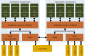
\includegraphics[width=0.6\columnwidth]{\chapterdirectory/figure/micro_bench/intel_nehalem.pdf}
\caption{%
Interconnected Intel Nehalem processors (extracted from \cite{10.1109/PACT.2009.22}).
}
\label{fig:micro_bench:intel_nehalem}
\end{figure}

\cite{10.1109/PACT.2009.22} is a paper on benchmarks performed on the Intel
Nehalem architecture (see Figure~\ref{fig:micro_bench:intel_nehalem}), which
uses the MESIF cache coherence protocol and has an inclusive cache hierarchy.
For clarification's sake, the cache coherence protocol is active below the L3
cache, meaning that this dual processor architecture effectively results in
only two caches being made coherent through MESIF.

To perform the benchmarks comparing the effect of coherence states of memory
element on writing and reading performance, their benchmark library makes it so
they are able to put data in the desired stable coherence state in the cache
they want, potentially using the other processor to attain the desired state.
In effect, this allows control of the coherence states of the system prior to
the start of the benchmark.  To reach the desired state in the caches of core
$N$, the following strategy is employed:
\begin{description}
\item[Modified] Core $N$ writes the data.
\item[Exclusive] Core $N$ writes the data (thus invalidating the other cores'
data), flushes, then reads the data.
\item[Shared] Core $N$ reaches the \textit{Exclusive} state, then another core
reads the same data.
\end{description}

There is an interesting omission: the \textit{Forward} state is not considered.
The authors indicate expecting the \textit{Forward} state to only become an
improvement for systems in which there are more than two processors and is thus
assumed not to have any effect on the benchmarks of their dual processor
architecture. This is incorrect, but, as explained later, the effects of the
\textit{Forward} are not seen in their results, since the benchmarks which would
have been affected were also omitted.

On the other hand, the strategy to reach a selected state for core $N$ described
above is still valid, even when ignoring the \textit{Forward}. Indeed, with this
process, the \textit{Forward} state only appears when reaching the
\textit{Shared} state, but it is reached by the core that ``reads the same
data'', not core $N$. In reality, having a \textit{Forward} state in an
architecture with only two caches does actually have some benefits: if the two
caches have read certain data, then one wants to write to it. Without
\textit{Forward} state, the cache wanting to write will have to fetch data in
RAM, whereas with the \textit{Forward} state available, it might be provided by
the other cache or simply ot have to fetch it in RAM (depending on which cache
performed a write first, and choices of implementation). Similarly, it has an
impact if a cache line is read by both caches, but the cache not in the
\textit{Forward} cache evicts it at some point, them re-acquires it. This would
have had an observable result when measuring the writing execution time. Indeed,
writing when core $N$ is in the \textit{Shared} state and another core is in the
\textit{Forward} state should result in faster execution time than when the other core
is in the \textit{Shared} state. Since The paper does not feature a table
proving a list of execution time when writing, but only for benchmarks that reading,
this difference cannot be seen and one might erroneously assume that the
\textit{Forward} state does indeed have no impact on systems with coherence
maintained between only two caches.

\iffalse
Considerations are taken to minimize any mechanic interfering with the
benchmarks: transaction look-aside buffers are pre-loaded and accessed memory
elements are not adjacent to avoid any pre-fetching optimization.
\fi

\begin{figure}[hbt!]
\begin{tabular}{cc}
\begin{subfigure}[t]{0.47\textwidth}
\lstinputlisting{\chapterdirectory/figure/micro_bench/algo_nehalem_latency.txt}
\caption{Latency benchmarks}
\label{fig:micro_bench:intel_nehalem_latency_algo}
\end{subfigure}
&
\begin{subfigure}[t]{0.47\textwidth}
\lstinputlisting{\chapterdirectory/figure/micro_bench/algo_nehalem_bandwidth.txt}
\caption{Bandwidth benchmarks}
\label{fig:micro_bench:intel_nehalem_bandwidth_algo}
\end{subfigure}
\end{tabular}
\caption{%
Algorithm overview for \cite{10.1109/PACT.2009.22} (taken from the paper)
}
\label{fig:micro_bench:intel_nehalem_algo}
\end{figure}

Figure~\ref{fig:micro_bench:intel_nehalem_latency_algo} shows an overview of the
algorithm used by \cite{10.1109/PACT.2009.22} to measure execution times. The steps
described are more about what is done prior to the measurements themselves.
Warming up the transaction look-aside buffer means pre-loading all entries in
order to avoid this loading being taken into account in the resulting execution time.
The accesses made for the measured part of the benchmark correspond to a pointer
chasing algorithm, just like in \cite{10.1145/2086696.2086713} (see
Figure~\ref{fig:micro_bench:co_running_apps_cots_algo_part_deux}).

The bandwidth benchmarking algorithm is shown in
Figure~\ref{fig:micro_bench:intel_nehalem_bandwidth_algo}. Synchronization
between the threads is more thoroughly controlled in this one: by memorizing the
exact window upon which each thread made its accesses, the window corresponding
to the period in which all threads were performing accesses can be obtained.
The bandwidth can then be obtained from the number of accesses successfully
performed within this window.

\begin{figure}[hbt!]
\centering
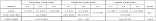
\includegraphics[width=\textwidth]{\chapterdirectory/figure/micro_bench/nehalem_read_latencies.pdf}
\caption{%
Latencies of reading from Core 0, results in ``nanoseconds (cycles)'' (Figure
taken from \cite{10.1109/PACT.2009.22})
}
\label{fig:micro_bench:intel_nehalem_read_latencies}
\end{figure}

Figure~\ref{fig:micro_bench:intel_nehalem_read_latencies} shows the results of
benchmarks measuring the time required for the core 0 to read data held in
various locations, according to the state of the data in the remote location.
Unsurprisingly, accesses made to the local L1 and L2 caches was not impacted by
the state of the data in the L3 cache. It appears this also holds true for the
local L3 cache itself. Access to data held in the caches of another core on the
same processor does vary depending on the coherence state. According to
\cite{10.1109/PACT.2009.22}, this is explained by the L3 cache having to check
on the L2 and L1 caches of that other core, as, unless the state is
\textit{Shared}, the L1 and L2 cores may hold a more up-to-date value. For data
held in the other processor, the results are as expected, with the cost of
traversing the bridge between both processors being added when accessing memory
elements in either the \textit{Exclusive} or \textit{Shared} state, but also
having a higher cost when accessing \textit{Modified} memory elements: as
explained in \cite{10.1109/PACT.2009.22} and Chapter~\ref{cha:cache_coherence},
\textit{Modified} memory elements are wrote back to the memory prior to being
sent as a reaction to a \textit{GetS} query.

\begin{figure}[hbt!]
\centering
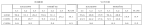
\includegraphics[width=\textwidth]{\chapterdirectory/figure/micro_bench/nehalem_bandwidths.pdf}
\caption{%
Bandwidth for access from Core 0, results in GB/s (Figure
taken from \cite{10.1109/PACT.2009.22})
}
\label{fig:micro_bench:intel_nehalem_broad}
\end{figure}

\cite{10.1109/PACT.2009.22} does however perform more analyses on the
performance of cache accesses. The second half of the paper is dedicated to
bandwidth analysis, of which the results are shown in
Figure~\ref{fig:micro_bench:intel_nehalem_broad}. These results are coherent
with their equivalent in the execution time benchmarks. They do provide more
information than what was available in the documentation however, such as actual
maximum bandwidth instead the theoretical maximal one.

The approach presented in \cite{10.1109/PACT.2009.22} is a good solution for the
\textit{benchmark} part of the framework described in
Section~\ref{sec:second_intro:framework}. Indeed, by taking into account the
coherence state of the targeted memory elements, \cite{10.1109/PACT.2009.22}
ensures the system state that led to the recording of the execution time is
understood and thus, that the correct execution time will be expected when attempting
to predict the architecture's behavior.
\stopallthesefloats

\stopallthesefloats{}
\section{Finding Elusive Hardware Monitors}
\label{sec:elusive_hardware_monitors}
\begin{figure}[hbt!]
\centering
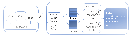
\includegraphics[width=\columnwidth]{\chapterdirectory/figure/micro_bench/expose_monitor_general_approach.pdf}
\caption{%
Trace collection process (extracted from \cite{palomo_et_al:LIPIcs:2020:12378})
}
\label{fig:micro_bench:expose_monitors}
\end{figure}

\cite{palomo_et_al:LIPIcs:2020:12378} presents a case study for the profiling of
architectures where performance monitors are not available. This is interesting,
because architecture profiling usually assumes that they are available. Having
a way to profile architectures without would extend the range of architectures
that can be considered for critical real-time contexts.

The architecture being studied in \cite{palomo_et_al:LIPIcs:2020:12378} is
system-on-chip with a dual-core processor.  While it does not have performance
monitors, it does have some hardware debugging features, which can be accessed
using a \textit{JTAG} port.

These hardware debugging features can snoop the messages passing through the
interconnect, as well as the instructions executed by each core (and their
program counter). In the approach proposed by
\cite{palomo_et_al:LIPIcs:2020:12378}, the platform is configured so that these
two sources of information are stored into circular buffers (within the chip).
The \textit{JTAG} connection is used to continuously copy these buffers into an
external analysis platform (see Figure~\ref{fig:micro_bench:expose_monitors}).
The speed at which these buffers are filled is higher than that of the
\textit{JTAG} connection, meaning that information would be lost if the programs
were running normally. Thus, the \textit{GRMON} script takes control of the
execution once the section of the programs under analysis is reached, and
proceeds to running the applications in a \textit{step-by-step} manner, which
ensures no information is lost.

Once this event capture is completed, the post-processing steps begin, starting
with a clean-up phase (\textit{Trace Merging}), which clears out redundant data.
Then comes the \textit{Event Counting} phase, which matches instructions to bus
events in order to recognize patterns that fit known events. For example, data
cache load misses are identified by seeing a load instruction be performed by
a core one cycle \textit{after} seeing the matching query go through the
interconnect.

Thus, instead of relying on performance counters, it is possible to obtain an
accurate description of the behavior of the platform through capture and
analysis of execution traces. Such strategies extend the range of platforms upon
which profiling is possible, including for the purpose of identifying cache
coherence using the process described in
Chapter~\ref{cha:identifying_cache_coherence}.

\stopallthesefloats{}
\section{Conclusion}
The approach shown in Section~\ref{sec:nehalem} is adequate for the second step
of the framework presented in this thesis (see
Section~\ref{sec:second_intro:framework}), in which the performance of the
architecture's cache coherence mechanisms are measured in order to feed them to
a model. Indeed, it does provide interesting information about single
instruction execution time according to the type of instruction being performed
(\loadinstr{} or \storeinstr{}) and the cache coherence state. It does not,
however, attempt to analyze the internals of the cache coherence mechanisms used
by the architecture. In fact, some of them are explicitly ignored
(\textit{Forward} state). Thus, while being an important step, it remains
insufficient to provide the user with enough information to understand what
interference could be generated by cache coherence mechanisms, unless the
identification step proposed in this thesis is applied.

Furthermore, approaches such as the one described in
Section~\ref{sec:elusive_hardware_monitors} can be used to apply the framework
presented in this thesis to architectures with more restricted monitoring
facilities.

\chapter{Handling Cache Interference in Safety-Critical Systems}
\label{cha:handling_it}
This chapter explores existing solutions to the issue of the interference
generated by cache coherence in safety-critical systems. Three approaches are
considered: Limiting either the capabilities of either the architecture or the
software running on it in order to limit the generation of these interference
(Section~\ref{sec:rel_work:handling_it:through_restrictions}); Modifying the
architecture's hardware or adding new hardware components in order to lessen
the unpredictability (Section~\ref{sec:rel_work:handling_it:through_hardware});
and lastly, solutions that involve running software in safety-critical systems
by showing that the effects of the interference remain acceptable.

\section{Through Restrictions}
\label{sec:rel_work:handling_it:through_restrictions}
The crudest approach to the handling of interference generated by cache
coherence is to not have any because all caches are disabled. While this
solution tremendously improves the predictability of the system, it also
tremendously decreases its execution speed, to the point where it may be
preferable to use a single-core architecture with caches instead.

One step above is a solution in which the caches are enabled, but their content
is locked, making their usefulness severely limited but without compromising the
system's predictability.

In this section are presented strategies that allow the use of caches in a
limited manner in order to achieve reasonable execution speed while keeping the
system as predictable as possible.

\subsection{Shared Cache Partitioning}
\cite{10.1145/1629335.1629369} presents two algorithms for a condition
sufficient to prove schedulability, it is meant for tasks with time and cache
space constraints in the context of a shared L2 cache in which space is
partitioned in order to avoid contentions.  Thus, this work is more about
proving that the measures taken in order to address interference are sufficient
rather than a strategy to control the interference itself. For these
schedulability tests, the tasks are assumed to be non-preemptive and to have a
fixed priority.

The paper's first algorithm is based on constraint programming. It basically
considers that there is a task missing its deadline, which implies that either
all cores are being used, or that too little cache space is available.
Intervals at which either of these conditions is true are searched for in order
to find their maximal impact of the hypothetical task that missed its deadline.
If this maximum impact is lower than the slack (longest affordable delay) of
this hypothetical task, then the tasks are schedulable. The second algorithm is
very similar, but simplifies the constraints by simply assuming the worst
possible interference from the other tasks in all criteria with much less
regard for whether the configuration leading to this interference is actually
possible. This effectively creates a more scalable schedulability test, at the
cost of being much more pessimistic.

\stopallthesefloats
\subsection{Cache Coloring to Curtain Interference}
\begin{figure}[hbt]
\begin{center}
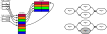
\includegraphics[width=\textwidth]{\chapterdirectory/figure/handling_it/cache_coloring_wcet.pdf}
\end{center}
\caption{Cache coloring aware scheduling, from \cite{DBLP:journals/corr/abs-1903-09310}}%
\label{fig:handling_it:cache_coloring}
\end{figure}
When using a set-associative cache, the cache is divided in equal sets of cache
lines. The memory element's physical address determines which of these sets of
cache lines it will go to. The cache eviction policy then applies solely inside
that set. The idea behind cache coloring is to exploit this, by determining
which memory element will find itself in which set of lines, and assigning
virtual addresses to physical addresses in a manner that will ensure a maximum
of virtual addresses will find themselves in the cache.

\cite{DBLP:journals/corr/abs-1903-09310} uses cache coloring in the opposite
manner. It instead assigns a single color (thus, set of cache lines) per
program. While this is not an efficient use of the cache for any one program,
it means that each program is effectively curtained into the set of caches of
its color. Using careful scheduling, the number of programs running in parallel
that share the same colors can be reduced (see
Figure~\ref{fig:handling_it:cache_coloring}), thus removing the interference
they can inflict on one another.
\stopallthesefloats

\subsection{Limited Shared Resources}
\begin{figure}
\centering
\includegraphics[width=0.6\columnwidth]{\chapterdirectory/figure/handling_it/marthy.png}
\caption{%
System running Marthy (Control Software in the figure), a figure extracted from
\cite{7311481}.
}
\label{fig:handling_it:marthy}
\end{figure}

One approach to dealing with cache coherence in multi-core processors for
environments requiring certification is to simply use the caches in a manner
that cancels the need for such a feature. Indeed, since the applications for
single core are already available, it stands to reason plenty of them could run
on multi-core processors without the need for shared memory elements. For
example, \cite{jean:tel-01341758} presents \textit{Marthy} (see
Figure~\ref{fig:handling_it:marthy}), a hypervisor aiming to enforce robust
partitioning between applications running on a COTS multi-core processor. This
hypervisor permanently lives in the cache of each core, using cache locking
mechanisms to avoid being inadvertently removed, and makes use of the MMU to
take over whenever an instruction triggers a cache miss, stalling that
instruction until access to the system's shared resources (i.e.~any shared
component, not just memory) is exclusively granted to the core by a TDMA. All
shared memory elements must be read-only, which does indeed remove the need for
cache coherence mechanisms.

\stopallthesefloats

\subsection{Isolated Communications Through Scheduling}
\begin{figure}
\centering
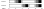
\includegraphics[width=0.5\columnwidth]{\chapterdirectory/figure/handling_it/deterministic_execution_model.pdf}
\caption{%
Overview of the strategy presented in \cite{10.1007/978-3-642-28293-5_9} (taken
from the paper)
}
\label{fig:handling_it:deterministic_execution_model}
\end{figure}

In \cite{10.1007/978-3-642-28293-5_9}, careful scheduling is used to make
calculating the worst-case execution time easier. This scheduling requires
programs running on each cores to have been sliced into computation blocks and
communication ones. Computation blocks are built so that while a core is in
one, the other cores cannot access the same data (or only as a read-only copy
if all tasks are only reading this data). Communications nodes indicate
fetching and writing periods (no computation), which are similarly limited by
any task currently performing a computation block. The paper provides a
strategy to automatically slice the programs intended for a core into a
scheduling of these types of blocks.
Figure~\ref{fig:handling_it:deterministic_execution_model} shows an example of
two cores having their tasks scheduled in this manner. White blocks indicate
time reserved for computation; grey blocks are for flushes; and black blocks
are for fetches.

Because they do not access any shared resource, calculating the worst-case
execution time of the computation blocks is equivalent to doing so on a single
core processor. \cite{10.1007/978-3-642-28293-5_9} proposes a solution for the
calculation of the worst-case time of communication blocks, including the
possibility for them to occur in parallel with other communication blocks from
other cores. It relies on the creation of a UPPAAL model to account for all
possible interleavings of any communications that may occur during that
particular communication block.  The aforementioned scheduling ensures that all
communications that can happen at that time are known.


\stopallthesefloats

% MARTI Xavier Jean, lock step stall access to the coherence until TDMA allows.
% Claire Pagetti: pre-fetch, then lock.
% See Quentin's Thesis for a desc of Pagetti's paper..


\section{Through Hardware Modifications}
\label{sec:rel_work:handling_it:through_hardware}
\subsection{Predictable MSI}
\label{sec:related_works:pmsi}
While not exactly a hardware modification per se, the use of a coherence
protocol designed for its predictability is not likely to be available on COTS
hardware, which is why the work presented in \cite{conf/rtas/HassanKP17} is
included in this section.

\cite{conf/rtas/HassanKP17} exposes the sources of unpredictability in the MSI
protocol, and proposes a solution for each one of them. These solutions require
some parts of the hardware connected to cache coherence mechanisms to be
predictable. Combined with, PMSI (Predictable MSI), the coherence protocol they
introduce, these solutions are indicated as sufficient to allow calculation of
the worst case delays that may be incurred by each instruction.

Translated to the formalism from Chapter~\ref{cha:cache_coherence}, the
restrictions imposed on the hardware are as follow:
\begin{enumerate}
\item
   Access to the interconnect is regulated by time slots. Caches may only send
   queries to the interconnect during their assigned time slot.
   \label{enum:pmsi_time_slot}
\item
   For a same memory element, the coherence manager sends replies to queries in
   the order of their arrival.
\item
   Caches reply to queries in the order of their arrival. This is equivalent
   to imposing $\cachedataoutfun{}$ to be a FIFO queue.
\item
   A write request to a cache for a memory element that it does not currently
   hold with read-and-write permissions can only occur during that cache's
   time slot.
   \label{enum:pmsi_write_time}
\item
   Writing to a memory element not currently held with read-and-write
   permissions requires all other caches' pending queries for that memory
   element to be processed first. Basically, the write is stalled if there
   are any queries in $\cachequeryinfun{}$ for that memory element.
   \label{enum:pmsi_ordering}
\item
   Caches are predictible in the ordering of their processing of instructions
   and external queries.
\end{enumerate}

\begin{figure}
\centering
\input{\chapterdirectory/figure/handling_it/pmsi_cache_controller.tex}
\caption{Split-Transaction PMSI Automaton for Cache Controllers}
\label{fig:pmsi_cc_table}
\end{figure}

\begin{figure}
\centering
\input{\chapterdirectory/figure/handling_it/pmsi_coherence_manager.tex}
\caption{Possible Split-Transaction PMSI Automaton for the Coherence Manager}
\label{fig:pmsi_mgr_table}
\end{figure}

Adapting \texttt{PMSI} to fit Chapter~\ref{cha:cache_coherence} is made easy by
the fact that they also based their description on the notations introduced in
\cite{Sorin:2011:PMC:2028905}. Figure~\ref{fig:pmsi_cc_table} shows how the
cache controller behaves for each memory element.  This figure is almost
identical to the one found in the paper presenting \texttt{PMSI}, with the
following modifications:
\begin{itemize}
\item
   A single \textit{Own Query} event is used instead of having
   one per type of query. This makes the table more compact, as there is never
   any state in which multiple categories of query have a different behavior
   when it comes to the handling observing their own queries on the
   interconnect.
\item
   The \texttt{Upg} query type, used to move from \texttt{S} to \texttt{M}, has
   been merged into \getmquery{}, as the differentiation did not appear to have
   any relevance to the protocol's behavior.
\item
   Emission of a \putmquery{} has been added as an action when receiving data
   in either \texttt{IM\textsuperscript{D}I} and
   \texttt{IM\textsuperscript{D}S}, as it would otherwise be impossible to exit
   the state they lead to. The need for this has been confirmed during exchanges
   with the authors.
\end{itemize}
\cite{conf/rtas/HassanKP17} does
not include a table for the coherence manager, which is instead simply described
as servicing the oldest pending query for a memory element every time it
receives data. Figure~\ref{fig:pmsi_mgr_table} shows a coherence manager that
would implement this behavior.

By comparison to the \texttt{MSI} protocol described in
Section~\ref{sec:split_msi}, \texttt{PMSI} features much fewer transient states.
This is because the restrictions imposed on the system have removed:
\begin{itemize}
\item The possibility of receiving a reply to a query not yet handled:
\texttt{IS\textsuperscript{BD}}, \texttt{IS\textsuperscript{B}},
\texttt{IM\textsuperscript{BD}}, \texttt{IM\textsuperscript{B}},
\texttt{SM\textsuperscript{BD}}, and \texttt{SM\textsuperscript{B}}.
\item Cache to cache data messages, which merge cases that were separated
because of whether data was sent only to another cache or also to the main
memory:
\texttt{IM\textsuperscript{D}SI}, \texttt{SM\textsuperscript{D}SI}.
\item Sending data as a reaction to seeing another cache's query:
\texttt{II\textsuperscript{B}} (now undistinct from
\texttt{MI\textsuperscript{B}}, which is now \texttt{MI\textsuperscript{WB}}).
\end{itemize}
In \texttt{PMSI}, receiving data for a memory element currently held in a cache
that may have modified it (e.g.~\texttt{M} state) always requires waiting for
that cache's time slot in the TDMA, as it will not perform a write back without
first broadcasting its own query indicating that it is about to do so. The cache
then sends a data message to the system's main memory, which only then is able
to reply to the original demand. While this is clearly penalizing in terms of
performance, it does lessen the variability in time required for acquisition of
data.

In conclusion, \cite{conf/rtas/HassanKP17} addresses the issue of the
predictability of memory access latency by replacing the cache coherence
protocol and performing some other hardware modifications in order to have
a generally slower but more easily computed and less fluctuating memory
access time. No modification of the software is required.

\stopallthesefloats

\subsection{Limited Cacheability}
\begin{figure}
\begin{center}
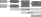
\includegraphics[width=0.5\textwidth]{\chapterdirectory/figure/handling_it/cacheability.pdf}
\end{center}
\caption{Cacheability Levels}%
\label{fig:handling_it:cacheability}
\end{figure}

One approach to the control of interference generated by cache coherence is to
limit which memory elements are affected by it. \cite{bansal2019cache} argues
for letting developers indicate, upon memory allocation, whether to allow the
new memory elements to be either cacheable as usual, not cacheable at all, or
only cacheable in caches shared by all cores (refered to as \texttt{INC-OC}).
Figure~\ref{fig:handling_it:cacheability} summarizes where memory elements can
be stored depending on the attribute they have been given.  \texttt{INC-OC},
which is the main contribution of the paper, is intended to remove these memory
elements from the cache coherence while not having to suffer the full cost of a
cacheless system upon their access. This does indeed result in more easily
predicted memory accesses for these particular memory elements, as they now
behave as they would in a single core system running concurrent programs:
another core/program may still evict them (either directly, or by allocating
more memory and triggering the automated eviction policy), but the possibles
system-wide states of those restricted memory elements (and thus possible
access latencies) are much fewer that they would otherwise be. This can thus
allow approaches for the analysis of memory latencies in single-core system to
be applied to these memory elements, a problem for which the available
literature is more prominent than for multi-core systems, with the added issue
of bandwidth sharing between the cores for access to that last-level cache.

As for limitations, the most oblivious one is that this is only applicable to
systems which do indeed implement a last-level cache being accessed by every
core. Furthermore, the addition of a new type of memory leads to hardware
modifications: translation look-aside buffers need to take into consideration a
new attribute, and so do all sent memory access queries. The authors argue that
some of these hardware modifications can sometimes be minimized through the use
of the architecture's instructions, and that this approach has the advantage of
being entirely orthogonal to the cache coherence mechanisms, thus not requiring
any modification of the admittedly complex coherence controllers.

In effect, the approach presented in \cite{bansal2019cache} requires some
hardware, as well minor operating system and hypervisor, modifications, in
order to let designers simplify the analysis, and lower the variation, of the
access time for any memory elements they choose. This does come at the cost of
the speed at which these memory elements are accessed, and it does require the
designer make a decision as to which memory elements should be handled this way.

\stopallthesefloats
\subsection{On-Demand Cache Coherence}
\begin{figure}
\begin{center}
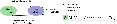
\includegraphics[width=\textwidth]{\chapterdirectory/figure/handling_it/odc2.pdf}
\end{center}
\caption{Overview of ODC\textsuperscript{2}, as seen in \cite{doi:10.1002/cpe.3172}.}%
\label{fig:handling_it:odc2}
\end{figure}

\cite{doi:10.1002/cpe.3172} presents ODC\textsuperscript{2} (On-Demand Coherent
Cache), a strategy to limit the interference of cache coherence on the
execution of real-time software (see Figure~\ref{fig:handling_it:odc2}). The
general idea is to have software delimit sections during which they access
shared data (\textit{Shared Mode}), and to have that shared data be evicted
from the cache as soon as the software leaves the section (\textit{Restore
Procedure}). Any new data loaded during Shared Mode is marked as being
\textit{shared} in the cache line, making their Shared data cannot be accessed
outside of these sections, which makes the code outside these coherence enabled
sections (called \textit{Private Mode}), much simpler to analyze.

A follow-up paper, \cite{Py2015.1}, performs the WCET analysis of some well
established algorithms (Dijkstra algorithm, Fast Fourier Transform, Matrix
Multiplication) by modifying an existing WCET computation framework (OTAWA) to
add support to ODC\textsuperscript{2}. The resulting WCET is compared with the
ones obtained when using no caches, when using \textit{Magic} (cache coherence
without any cost, which represents the best theoretical performance), and an
approach that simply invalidates the full cache upon entering any
synchronization point. The results show, somewhat unsurprisingly,
ODC\textsuperscript{2} obtains a lower computed WCET than the other approaches,
\textit{Magic} excepted.

\stopallthesefloats{}

\subsection{Dynamic Verification of Cache Coherence}
\begin{figure}
\begin{center}
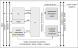
\includegraphics[width=0.7\textwidth]{\chapterdirectory/figure/handling_it/dynamic_verification.pdf}
\end{center}
\caption{Overview of the altered cache, as seen in \cite{Cantin2004DynamicVO}.}%
\label{fig:handling_it:dynamic_verification}
\end{figure}

\cite{Cantin2004DynamicVO} proposes a strategy to implement fault detection in
cache coherence systems, addressing both permanent and temporary issues by
adding hardware (See Figure~\ref{fig:handling_it:dynamic_verification}) that
replicates a simplified version of the cache coherence logic and tests it for
consistency with the real one.

The approach proposed by \cite{Cantin2004DynamicVO} recommends the addition
of a new interconnect dedicated to the validation of the cache coherence
protocol, to avoid disrupting the existing one. This new interconnect is solely
used by caches to broadcast that they entered a stable state for a given memory
element so as to allow the other caches to check that their local state for that
memory element is not in conflict with the broadcasted one. For example, if a
cache broadcasts that it has reached the $M$ state for a memory element, then
all other caches seeing that broadcast would test that they do not have that
memory element in any state other than $I$.

This new verification performed on each cache partaking in the coherence
protocol requires the addition of some hardware to each cache. In addition to
checking for consistency with the other caches through broadcasts, this new
hardware maintains a simplified version of the coherence state of each memory
element. It does not incorporates transient states and, since it only considers
state changes and whether they allow a given instruction to be performed, the
resulting coherence protocol is that of one operating on an atomic interconnect
with atomic operations (such as the one in Section~\ref{sec:intro_to_msi}).
In effect, the simplified protocol only sees events once the transaction they
were part of has been completed. At that point, it receives address, event,
initial and final stable state and compares these with its own record. To detect
timeout issues, a watchdog is also added to the caches.

Thus, while it requires rather complex hardware modifications,
\cite{Cantin2004DynamicVO} does provide a way to detect the occurrence of errors
in the cache coherence protocol's behavior.

\stopallthesefloats{}

% Configuration, lock, set as uncacheable.

\section{By Accepting It}
\label{sec:rel_work:handling_it:accepting_it}
The most common approach to the analysis of interference in caches relies on
the static analysis and abstract interpretation approach originating from
\cite{10.1023/A:1008186323068}, which categorized accesses to caches depending
on whether they always found the value, never did, or if that could not be
determined. This was then taken into account account for the computation of the
WCET. The publications that followed usually propose the addition of a new
categorization, or remark on the incorrectness or incompleteness of the way
these categorizations evolve during the analysis of the program's CFG, and
propose corrections for mistakes made on previous attempts at doing so (up to,
and including, what has been presented in \cite{10.1023/A:1008186323068}).
While otherwise prevalent, this particular approach is not the one focused on in
this thesis, and thus only very few of these papers have been included in this
section. Readers interested in learning more about this subject are encouraged
to read \cite{10.1145/3290367}, and especially its well presented related works
section.

\subsection{Instruction Cache Analysis}
Most papers handling WCET analysis on multi-cores only consider instruction
caches, bypassing the need to address cache coherence by indicating that
instructions cannot be modified. While this makes them slightly outside the
scope of this thesis, the sheer prevalence of this restriction in WCET papers
would make their complete omission feel amiss.


\stopallthesefloats
\subsubsection{WCET analysis}
\begin{figure}[hbt]
\centering
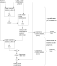
\includegraphics[width=0.65\columnwidth]{\chapterdirectory/figure/handling_it/bypass_to_wcet.pdf}
\caption{%
Overview of the strategy presented in \cite{10.1109/RTSS.2009.34} (taken
from the paper)
}
\label{fig:handling_it:bypass_to_wcet}
\end{figure}

\cite{10.1109/RTSS.2009.34} proposes a way to compute WCET for multi-core
architectures, with considerations for shared instruction caches with multiple
levels of hierarchy. It also tries out a \textit{bypassing scheme}, which
relies on the identification of single-use program blocks within shared
instruction caches to compile programs in a way that reduces interference
between tasks.

The proposed WCET computation strategy is based on existing approaches for
multi-levels instruction caches in single core processors. It uses static
analysis to categorizes all accesses as either: always-miss, always-hit,
first-miss (first access is unknown, but all following accesses will hit), and
not classified (for accesses that fail to be categorized in the other
patterns). This categorization (referred to as \textit{CHMC} in the paper) is
done for every cache level. Furthermore, the likeliness of an access actually
reaching a level is also evaluated and categorized with similar labels (always
acceded, never, always after the first access, unknown). Moving this strategy
to multi-core processors is indicated as having the potential of changing some
always-hit and first-miss into first-miss and \textit{not classified}. Accesses
made by different tasks on the same level where the categorization indicates
that the access is not \textit{never} done are considered as interfering with
one another (regardless of when the accesses are made). This is then used to
re-evaluate the hit/miss categorization so that it has the interference taken
into account. The result of the interference identification analysis is referred
to as \textit{C}ache block \textit{C}onflict \textit{N}umber. To improve the
precision of the result, the possibility of having code shared among tasks
(such as libraries) is taken into account. An overview of the whole process for
a given cache level $\ell$ is shown in
Figure~\ref{fig:handling_it:bypass_to_wcet}.

The decisions made in what to cache generally follow the
locality of reference principle, where the proximity of elements in memory is
assumed to translate to a proximity is usage times, and that processors
receptively access the same elements within short time periods. In
\cite{10.1109/RTSS.2009.34}, static analysis is used to find elements which are
only used once (called \textit{S}tatic \textit{S}ingle \textit{U}sage), in
order to avoid having them pollute caches and risk being considered as a source
of interference needlessly. This relies on a bypass mechanism, that allows
fetching data without altering the caches: if it is not found within any cache,
the value is retrieved but not added to any cache; if it is found within a
cache, the caches in-between do not get any copy, and the copy that was used is
not updated to indicate a recent access.
\stopallthesefloats


\stopallthesefloats

\subsubsection{Unified WCET Analysis Framework}
\begin{figure}
\centering
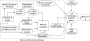
\includegraphics[width=\columnwidth]{\chapterdirectory/figure/handling_it/chattopadhyay_wcet.pdf}
\caption{%
Overview of the strategy presented in \cite{10.1145/2584654} (taken from the
paper)
}
\label{fig:handling_it:chattopadhyay}
\end{figure}
\cite{10.1145/2584654} presents a framework for WCET analysis on multi-core
platforms, which distinguishes itself from other solutions by the number of
features it takes into consideration. Indeed, the framework accounts for shared
caches, pipelines, and branch prediction. It also does not require the
assumption of a timing-anomaly-free architecture. An architecture free of
timing anomalies are architectures for which performing an operation faster on
a core cannot result in a longer execution time for the program compared to if
that operation took longer. The oppose would, for example, if the instruction
activates cache coherence mechanisms which would not have been necessary if the
in faster execution of that instruction. Readers interested in more possible
causes for timing anomalies are encouraged to read
\cite{DBLP:conf/wcet/ReinekeWTWPEB06}).
Figure~\ref{fig:handling_it:chattopadhyay} provides an overview of the
approach.  The assumptions that it does are as follow: use of a TDMA-based
round-robin arbitration policy, cores each have a private L1 cache. Data and
instructions are assumed to be fully separated (separate caches, separate
buses). Only instruction caches are taken into account (no cache coherence, no
possibility of modifications). Caches are assumed to be non-inclusive and to
use the LRU replacement policy.

The approach analyzes the WCET for each core separately.  Using abstract
interpretation, memory accesses are categorized according to whether they
always hit, always miss, or are marked as being unclassified. This is done for
both the L1 and L2 caches. The L2 cache can be a shared one, in which case
accesses susceptible to inter-core interference may move from always hits to
unclassified. This inter-core interference appears to be the only considered
direct interference from other cores, due to the assumptions made on the
architecture. Speculative execution, the result of branch prediction, may also
have effects on the contents of the L1 and L2 caches, as well as the pipeline's
behavior. A model of the shared bus's TDMA is taken into account when creating
the pipeline's model, adding a latency to certain stages. This pipeline model
creation process appears to be fairly complex, proceeding in an iterative
manner to compute the WCET of each basic computation block. Having the WCET of
each basic block, a model of the branch prediction mechanics and that of the
TDMA are used in the definition an linear optimization objective that will
return the WCET of the whole program.


\stopallthesefloats
\subsection{Data Cache Analysis}
\subsubsection{Bypass Heuristics}
\cite{lesage:inria-00531214} uses a similar approach to
\cite{10.1109/RTSS.2009.34}, this time focusing on data caches instead. Cache
coherence protocols are not considered. Indeed, all accesses to shared data is
assumed to bypass private caches (something that could be implemented by
\cite{bansal2019cache}, for example) and all shared-caches are assumed
to be write-through. Data and instructions are assumed to not interfere with
each other. In effect, the main change from what is presented in
\cite{10.1109/RTSS.2009.34} is how accesses to a memory bock are determined:
in the case of an instruction cache, a single instruction always points to
the same memory blocks; whereas in data caches, the relation between instruction
and memory block is murkier, as addresses may be aliased. This makes the
detection of Static Single Usage cache blocks, which were the target of bypass
mechanisms in \cite{10.1109/RTSS.2009.34}, much more complex. Multiple
heuristics on which elements to bypass at shared cache level $\ell$ are
provided: any instruction for which none of the targeted memory references have
statically been detected to be leading to a sure hit in $\ell$ in the future;
any instruction for which the target cannot be statically computed, in order to
increase determinism; and one that bypasses any access of a task until it only
occupies a given number of cache ways, which allows for conflict reduction
through control of the maximum occupied space by each task.


\subsubsection{Write-Back Data Caches}
\cite{10.1145/3139258.3139269} tackles the issue of WCET computation in
multi-core processors that use data (or unified) shared caches with write-back
policies. Although not explicitly stated in the paper, this approach does not
consider separate caches of the same hierarchy: all caches are shared by all
cores that could access the data they contain. Ergo, no cache coherence, but a
cascade of non-inclusive shared caches.

In addition to the standard categorization of a cache line in a particular
cache level (always hits, never hits, and so on\ldots), the \textit{dirtiness}
is also modeled. The possible values are: dirty (i.e.~has been written to, but
changes were not yet propagated), clean, or possibly dirty. The main challenge
is then to estimate when the write back will occur.
\cite{10.1145/3139258.3139269} indicates how to take this new attribute into
account when performing the usual cache static analysis, and the constraints it
adds to the linear optimization problem representation of the WCET computation.




\stopallthesefloats
\section{Conclusion}
\section{Conclusion}
This chapter has shown how UPPAAL's model checking capabilities can be exploited
to analyze the interference caused by cache coherence on the model from
Chapter~\ref{cha:modeling_cache_coherence}.

This analysis starts by a computation of the WCET for each program. Useful in
itself, this analysis is extended by that of the WCET for these programs with
the architecture in different configurations in order to extract more
information about how much of the execution time is caused by interference.

In order to more precisely understand what determine the WCET and to provide
the user with information about elements of the program that can directly be
manipulated, the analysis proceeds by an categorization of the accuracy of each
instruction. This indicates which instructions are unaffected by the
interference, which instructions are always time-consuming, and which
instructions take a varying amount of time depending on the execution. By
looking at the accuracy of all accesses made on each memory element, patterns
for these instructions of varying execution time can sometimes be found, which
results in a more predictable system.

The determining factor for the accuracy of instructions is then properly
defined. This corresponds to a categorization of all external queries depending
on their effects on the permissions held by a cache, and whether a loss of
permission led to an instruction taking additional time. Thus, three categories
of interference are defined: minor (no change of permission, but loss of time
due to query processing), demoting (loss of writing permission), and expelling
(loss of all permissions).

Finally, analyses are performed in order to determine how each instruction
interfere with the other instructions. This results in a graph showing, for
each instruction, which instruction can generate interference that will
directly impact it, the category of this interference, and whether this
interference occurs on all possible executions or not.

This provides the user with a clear understanding of the causes and effects of
cache coherence interference on the programs' instructions, opening the way to
finding means of mitigation for this interference.


\chapter{Analyzing Performance Through Formal Methods}
\label{cha:analyzing_rel_work}
The most common use of formal methods in relation to cache coherence is to
validate protocol correctness (i.e.~that a protocol verifies the properties set
in Section~\ref{sec:proper_cache_coherence_protocol}).  Indeed, the use of model
checking for that purpose is the source of many publications. For example,
\cite{conchon13jfla} describes a parameterized model checker by focusing on the
verification of a cache coherence protocol, by taking its description from yet
another paper using model checking to verify it (\cite{Baukus2002}) and thus
allowing a comparison between the approaches.

However, proving the correctness of a cache coherence protocol is not the
subject of this thesis. We assume the protocols to be correct, and are instead
interested by the impact the cache coherence has on the real-time properties
of the system. Thus, in chapter, we look at real-time systems using
formal methods to analyze the real-time properties of an architecture. As this
is a fairly restrictive criterion, the results include approaches meant for
single-core processors in addition to those for the more on-topic multi-cores.

\section{Single-Core Processors}
\stopallthesefloats
\subsection{METAMOC}
\begin{figure}[hbt]
\begin{center}
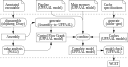
\includegraphics[width=\textwidth]{\chapterdirectory/figure/analysis/metamoc.pdf}
\end{center}
\caption{Using METAMOC to compute WCET (from
\cite{dalsgaard_et_al:OASIcs:2010:2831})}%
\label{fig:formal_analysis:metamoc}
\end{figure}

The first tool that made use of UPPAAL for the computation of WCET by modeling
hardware was Modular Execution Time Analysis using Model Checking (METAMOC),
introduced in \cite{dalsgaard_et_al:OASIcs:2010:2831}. The general idea behind
the approach is shown in Figure~\ref{fig:formal_analysis:metamoc}. The
modularity can clearly be seen in how the models for the cpu pipeline,
main memory, and cache specifications are kept separate in order to facilitate
their replacement when analyzing for a different processor. The other input is
that of the analyzed executable, directly in its binary form, albeit with some
annotations regarding loop bounds.

Given these inputs, METAMOC generates a control flow graph for the program,
which is in fact yet another UPPAAL model to combine to the ones representing
the architecture. The value analysis statically determines the address of
memory elements, and is disabled if the modeled architecture does not feature
any data cache.

The pipeline model corresponds to a collection of automata, one for each stage:
\textit{fetch}, \textit{decode}, \textit{execute}, \textit{memory}, and
\textit{writeback}. The parallel nature of pipelines translates fairly well
into a network of automata communicating through channels, making the writing
of such automata accessible for the user wanting to add their own in hopes of
modeling another architecture. The main challenges then come in determining
what can stall the pipeline on the real architecture and how long each stage
should take. Indeed, the authors of \cite{dalsgaard_et_al:OASIcs:2010:2831}
indicate that the documentation for the processor they modeled explicitly
states that it does not contain an exhaustive list of all possible stalls.

The default model for caches considers separate instructions and data caches,
matching the architecture they made their approach around. Caches are
set-associative, and implement an LRU eviction policy.

\begin{figure}[hbt!]
\begin{center}
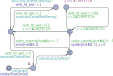
\includegraphics[width=0.8\textwidth]{\chapterdirectory/figure/analysis/half_metamoc_cache.pdf}
\end{center}
\caption{Half of Cache in METAMOC (adapted from \cite{dalsgaard_olesen_toft_2020})}%
\label{fig:formal_analysis:metamoc_caches}
\end{figure}

Figure~\ref{fig:formal_analysis:metamoc_caches} shows one half of the automaton
modeling a cache in METAMOC. The complete automaton has a second half mirroring
this one, with \textit{read} instead of write. Upon receiving a request for
a cache write, the automaton determines from its internal state whether the
request is a cache hit or if the instruction must be added to the cache. This
corresponds to \lstinline{cache_contents(instrArd)} being equal to -1 (cache
miss) or not (cache hit). In the case of a cache hit, a delay corresponding to
the time spent writing in the cache is introduced (controlled by
the \lstinline{CACHEFETCH} clock). \lstinline{write_hit_wait} corresponds to
the number of main memory accesses to be performed. Such accesses can still
occur even after a cache hit, if a write-through policy is in place. In the
case of a cache miss, a number of accesses to the main memory are performed.
This number can be higher than one if a cache line had to be evicted and the
cache follows a write-back policy. Once all accesses are performed, the cache
synchronizes on \textbf{instructionCacheWrite} to indicate that the request
was completed.

\begin{figure}[hbt!]
\begin{center}
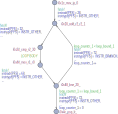
\includegraphics[width=0.8\textwidth]{\chapterdirectory/figure/analysis/metamoc_prog.pdf}
\end{center}
\caption{Fragment of Program Automaton in METAMOC (from \cite{dalsgaard_olesen_toft_2020})
}
\label{fig:formal_analysis:metamoc_program}
\end{figure}

Figure~\ref{fig:formal_analysis:metamoc_program} shows an example fragment of
an automaton corresponding to a program after processing by METAMOC. The
fragment in question corresponds to a loop, and shows how METAMOC supports
branching and iterating. The \textit{loop\_counter\_1} and
\textit{loop\_bound\_1} variables ensures that its execution terminates. The
bounds of such loops have to be annotated in the program's source code.

Their solution to limit search-space explosion is to put a caveat stating that
the architectures are assumed to be time-anomaly free, which lets them consider
only the locally worst time for some operations, instead of having to explore
all possible timings in case a better local time leads to a globally worse one.

\stopallthesefloats

\stopallthesefloats
\subsection{WUPPAAL}
\begin{figure}[hbt]
\begin{center}
\centering
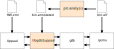
\includegraphics[width=0.7\textwidth]{\chapterdirectory/figure/analysis/wuppaal.pdf}
\end{center}
\caption{Overview of WUPPAAL's components (taken from \cite{wuppaal})}%
\label{fig:formal_analysis:wuppaal}
\end{figure}

\cite{wuppaal} describes WUPPAAL, another approach to using UPPAAL in order to
compute the WCET of a program running on a single-core processor. The main
novelty of \cite{wuppaal} is that it combines simulated execution with the
model checking. Indeed, as can be seen in
Figure~\ref{fig:formal_analysis:wuppaal}, it allows UPPAAL to interact with
\textit{qemu} (an architecture simulation tool) through \textit{gdb} (a
debugging tool) and \textit{libgdbuppaal} (a library of their own making). The
\textit{pre-analysis} step shown in the figure corresponds to the annotation of
a binary program with information in order to help the extraction its
\textit{Control Flow Graph}. This approach aims at improving the memory usage
of model checking, as well as making the approach fit other architectures very
easily (by just changing qemu parameters).

These annotations allow the generation of an over-approximation of all valid
program runs from the CFG. This has some surprising results, such as
deterministic programs having multiple separate runs because the
over-approximation does not consider actual values for any computation
involving input parameters. Instead, all outcomes are considered, even if some
sequences of outcomes cannot follow one another (e.g.~the exact same test
failing once, then succeeding). For such runs to be finite, loops cannot be
controlled by input parameters (i.e.~all loops have a known amount of
iterations).

\begin{figure}[hbt]
\begin{center}
\centering
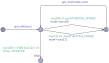
\includegraphics[width=0.7\textwidth]{\chapterdirectory/figure/analysis/wuppaal_automaton.pdf}
\end{center}
\caption{Automaton interacting with \textit{libgdb2uppaal} (taken from
\cite{wuppaal})}%
\label{fig:formal_analysis:wuppaal_automaton}
\end{figure}

UPPAAL is used to perform queries among all possible execution paths. However,
in WUPPAAL, the automaton corresponding to the program is not a purely UPPAAL
one. Figure~\ref{fig:formal_analysis:wuppaal_automaton} shows the automaton in
question.  It does not store full program states, and instead only keeps an
identifier and the annotations for current instruction. The function calls seen
on the automaton actually trigger another component from
Figure~\ref{fig:formal_analysis:wuppaal}: \textit{libgdbuppaal}. This component
is where program states are stored. \textit{libgdbuppaal} uses \textit{qemu} to
compute the program state resulting from the application of the instruction, as
well as all possible next execution nodes. The program state inserted back in
UPPAAL indicates whether the instruction was found in the cache and how long its
execution stage lasts.

UPPAAL is then involved in the computation of the WCET for these annotated
traces. Indeed, it models the pipelines, with one automaton per stage, as well
as a main memory automaton and an instruction cache one (see
Figure~\ref{fig:formal_analysis:wuppaal_cache}), to model their access times.
Since the information about whether the instruction cache contains the
instruction or not is already in the annotated execution trace, these last two
automata are kept very simple.

\begin{figure}[hbt]
\begin{center}
\centering
\includegraphics[width=0.7\textwidth]{\chapterdirectory/figure/analysis/wuppaal_cache.pdf}
\end{center}
\caption{WUPPAAL Instruction Cache Automaton (taken from
\cite{wuppaal})}%
\label{fig:formal_analysis:wuppaal_cache}
\end{figure}

Figure~\ref{fig:formal_analysis:wuppaal_cache} shows the automaton
corresponding to an instruction cache in WUPPAAL. The initial state is the top
one. Upon receiving a request for reading on \textbf{InstructionCacheReadStart}
(considering the rest of the variables, writing likely uses the same channel),
the automaton checks if the information is already in the cache. If not it
performs as many synchronizations with the main memory automaton as is needed
(indicated by \textit{PMT}), then waits a time corresponding to that of a
cache access before using \textbf{InstructionCacheReadEnd} to signal the
completion of the request.

\stopallthesefloats


\section{Multi-Core Processors}
\stopallthesefloats{}
\subsection{Modeling Shared Buses}
\begin{figure}[hbt!]
\begin{center}
\includegraphics[width=0.7\textwidth]{\chapterdirectory/figure/analysis/mingsong.pdf}
\end{center}
\caption{Overall strategy for \cite{5702243} (taken from the paper)}%
\label{fig:formal_analysis:mingsong}
\end{figure}

The approach proposed by \cite{5702243} combines abstract interpretation and
model checking to compute WCET in multicore, with a special focus on the
interconnect. The abstract interpretation is found in the analysis of the
caches, which is done in a fashion similar to those presented in
Section~\ref{sec:rel_work:handling_it:accepting_it}, including in its remarks
of a previous approach being unsafe and in its omission of data caches (and
thus, of cache coherence). The overall strategy for this approach is shown in
Figure~\ref{fig:formal_analysis:mingsong}.

\begin{figure}[hbt!]
\begin{center}
\includegraphics[width=\textwidth]{\chapterdirectory/figure/analysis/mingsong_program_block.pdf}
\end{center}
\caption{Program Model Building Blocks (taken from \cite{5702243})}%
\label{fig:formal_analysis:mingsong_prog_blocks}
\end{figure}

\begin{figure}[hbt!]
\begin{center}
\includegraphics[width=\textwidth]{\chapterdirectory/figure/analysis/mingsong_program.pdf}
\end{center}
\caption{Program Example (adapted from \cite{5702243})}%
\label{fig:formal_analysis:mingsong_program}
\end{figure}

The resulting model considers program instructions only as their categorization
(\textit{Always Hits}, \textit{Always Misses}, \textit{First time Misses},
\textit{Not Categorized}). The paper proposes an automaton for each category
(see Figure~\ref{fig:formal_analysis:mingsong_prog_blocks}),
indicating how an instruction of this category will use the
interconnect. Models for program are thus constructed by replacing each
instruction in the control flow graph by the automaton corresponding to its
synchronization with the interconnect
(\textit{TA Construction} in Figure~\ref{fig:formal_analysis:mingsong}). An
example of resulting automaton can be seen in
Figure~\ref{fig:formal_analysis:mingsong_program}.

To showcase how modular the approach is in its modeling of the interconnect,
\cite{5702243} provides both a model for a TDMA bus and for a FCFS
(\textit{First Come, First Served}, which means requests are completed in the
order of their arrival) bus.

Figure~\ref{fig:formal_analysis:mingsong} mentions an ILP model being computed
as well, however, the paper does not make any mention of it.

\stopallthesefloats{}

\stopallthesefloats
\subsection{Multi-Core Analysis using only UPPAAL}
The authors \cite{conf/wcet/GustavssonELP10} present an approach using UPPAAL
to perform computation of the worst-case execution time for software running
on multi-core processors. While it does not feature cache coherence, it does
support hierarchical (and shared) caches, as well as some sort of instruction
pipelining.

\begin{figure}[hbt!]
\begin{center}
\includegraphics[width=\textwidth]{\chapterdirectory/figure/analysis/gustavsson_prog.pdf}
\end{center}
\caption{Program Automaton (taken from \cite{conf/wcet/GustavssonELP10})}%
\label{fig:formal_analysis:gustavsson_program}
\end{figure}

In \cite{conf/wcet/GustavssonELP10}, programs are represented by their own
automata (See Figure~\ref{fig:formal_analysis:gustavsson_program}), sending
instructions through shared variables by synchronizing with a core on
a dedicated channel. This approach allows programs to feature branching and
non-memory-related instructions, by simply adding numerical variables and
making the automaton more than a simple sequence of states. In
Figure~\ref{fig:formal_analysis:gustavsson_program}, the framed part corresponds
to where the program's instruction graph should be. The \textit{id} variable
targets a particular core on which to execute the instruction, and
\textit{set\_access\_info} populates the global variables characterizing the
instruction: \textit{instr\_address} for the address of the instruction in the
modeled memory, \textit{data\_address} for the address of any data being
accessed, \textit{data\_access} to indicate if this instruction accesses data,
and \textit{write\_data} to differentiate between a read and a write access.
The \textit{Terminating Synchronization} part is here to ensure the task is not
considered completed until it has indeed completed all accesses for its final
instruction (and not just sent the instruction).

Cores are modeled as automata that go through the pipeline required for an
instruction to be completed, which includes accessing the instruction cache as
well as, potentially, the data cache. Interestingly enough, this model does not
use one automaton per stage of the pipeline. Instead the whole core logic is
modeled in a single automaton.


\begin{figure}[hbt!]
\begin{center}
\includegraphics[width=\textwidth]{\chapterdirectory/figure/analysis/gustavsson_caches.pdf}
\end{center}
\caption{Cache Automata (taken from \cite{conf/wcet/GustavssonELP10})}%
\label{fig:formal_analysis:gustavsson_caches}
\end{figure}

Each L1 instruction cache has its own automaton, managing the possibility for
instructions to have already been cached or sending a request for that
instruction to the L2 cache. The L1 data caches are similar (see
Figure~\ref{fig:formal_analysis:gustavsson_caches}), with the added possibility
of writing data to a memory element, which invalidates it from every other L1
data cache.

The automaton for the L2 cache is very straightforward, a simple loop going
over each request, determining whether the data is supposed to be in the L2
cache or not, and delaying the reply accordingly.

\iffalse
An extra automaton is also provided, which acts as a mutex for use in modeling
the programs.
\fi

Unsurprisingly, the hampering factor is scalability when the number of modeled
cores is increased. There appear to have very little in the way of synchronicity
between the cores (such as using a round-robin for L2 cache accesses), which
is likely to be aggravating the issue.
\stopallthesefloats


\section{Conclusion}
This chapter has shown how UPPAAL's model checking capabilities can be exploited
to analyze the interference caused by cache coherence on the model from
Chapter~\ref{cha:modeling_cache_coherence}.

This analysis starts by a computation of the WCET for each program. Useful in
itself, this analysis is extended by that of the WCET for these programs with
the architecture in different configurations in order to extract more
information about how much of the execution time is caused by interference.

In order to more precisely understand what determine the WCET and to provide
the user with information about elements of the program that can directly be
manipulated, the analysis proceeds by an categorization of the accuracy of each
instruction. This indicates which instructions are unaffected by the
interference, which instructions are always time-consuming, and which
instructions take a varying amount of time depending on the execution. By
looking at the accuracy of all accesses made on each memory element, patterns
for these instructions of varying execution time can sometimes be found, which
results in a more predictable system.

The determining factor for the accuracy of instructions is then properly
defined. This corresponds to a categorization of all external queries depending
on their effects on the permissions held by a cache, and whether a loss of
permission led to an instruction taking additional time. Thus, three categories
of interference are defined: minor (no change of permission, but loss of time
due to query processing), demoting (loss of writing permission), and expelling
(loss of all permissions).

Finally, analyses are performed in order to determine how each instruction
interfere with the other instructions. This results in a graph showing, for
each instruction, which instruction can generate interference that will
directly impact it, the category of this interference, and whether this
interference occurs on all possible executions or not.

This provides the user with a clear understanding of the causes and effects of
cache coherence interference on the programs' instructions, opening the way to
finding means of mitigation for this interference.




   \part{Contributions}
   \chapter{Identifying Cache Coherence}
\label{chap:identifying_cache_coherence}
\label{cha:identifying_cache_coherence}
\definechapterdirectory{src/identifying}

\stopallthesefloats
The introduction of multi-core processors in critical avionic systems requires
the ability to sufficiently predict their behavior so that certification of the
system is achievable. Indeed, the parallel nature of multi-core processors
leads to numerous interactions that do not strictly pertain to the objective
of the applications being ran. This large amount of unprompted interactions
render execution times difficult to predict and subject to large variations.
Among the main causes of large time variations is cache coherence, the
mechanism ensuring that data modifications performed by programs running in
parallel are properly propagated. While cache coherence can be implemented with
predictability in mind (see
Section~\ref{sec:rel_work:handling_it:through_hardware}), this requires hardware
modifications, precluding such solutions in an aeronautical context.
Unfortunately, the available strategies to predict worst-case execution time of
applications running on multi-core \textit{Commercial Off-The-Shelf} processors
require cache coherence to be deactivated (see
Section~\ref{sec:rel_work:handling_it:accepting_it} and
Chapter~\ref{cha:analyzing_rel_work}).

This thesis proposes solutions to begin addressing the issue of cache coherence
predictability in an aeronautical context. To do so, it provides the applicant
with tools that can expose and explain the interference generated by cache
coherence. In this chapter is provided a summary, the limitations, and
suggestions of future improvements for each contribution made in this thesis.

\stopallthesefloats
\section{Identification Strategy}
\label{sec:identification:strategy}
This section presents the strategy used to identify the cache coherence protocol
of an architecture. As a reminder from Chapter~\ref{cha:cache_coherence}, cache
coherence protocols are defined around a single memory element. Thus, the
identification strategy only considers a single memory element in its process.
Moreover, the following hypotheses are made:
\begin{itemize}
\item
   The architecture encodes stable cache states using binary flags attached to
   each cache line (see
   Definition~\ref{def:identifying:cache_controller_state}).
\item
   The user is able to observe cache line attributes (at least the
   aforementioned binary flags and the associated memory element address).
\end{itemize}
\iffalse
Because the user's means of observation are likely to be incomplete, there is
no way to ensure all behaviors of the protocol can be identified: there is
always the possibility of the architecture's cache coherence protocol relying
on something that cannot be observed.
\fi
In effect, this identification strategy tests whether, as far as the user's
observation capabilities allow, the architecture's cache coherence protocol
implements all (and only) the behaviors of the hypothetical cache coherence
protocol. The identification strategy is split in several steps, described
hereafter.

\subsection{Defining the Hypothetical Cache Coherence Protocol}
The first step is to define the hypothetical cache coherence protocol using the
notation presented in Chapter~\ref{cha:cache_coherence}. A good starting point
is to use the information available in the architecture's documentation in order
to know which cache coherence protocol to define.

Taking for example the NXP QorIQ T4240 architecture, the user would consult the
architecture's documentation \cite{T4240}. This document does not indicate the
cache coherence protocol in use on the architecture. However, it does mention
\textit{cache intervention}: queries which generate a cache hit on another cache
can be made to provide the data reply. Reading on the core's documentation
\cite{e6500}, the L2 cache coherency model is indicated to be the MESI protocol.
As a result, in this case, the hypothetical cache coherence protocol would be
a MESI protocol.

\subsection{Defining the Observable Cache Coherence Protocol}
The observable cache coherence protocol is the amalgam of the results from each
performed benchmark. This subsection defines each relation involved in the
observable protocol, and points out their equivalent from
Chapter~\ref{cha:cache_coherence}, when applicable. Indeed, the definitions from
Chapter~\ref{cha:cache_coherence} cannot be re-used as-is for the observed cache
coherence protocol, because the observations are done on binary flags and
performance monitors, whereas the notations in Chapter~\ref{cha:cache_coherence}
are more abstract.

\begin{definition}[Observable Coherence State]
\label{def:identifying:cache_controller_state}
   On a real architecture, each line of a cache or coherence manager has
   \archboolflagscount{} binary flags providing information on its state.
   We can then define $\cacheboolstatefun{}: \caches{} \to
   \memoryelements{} \to \archboolflags{}$, which indicates the valuation
   of these binary flags for a given memory element (see
   Definition~\ref{def:memoryelement}) in a given cache (see
   Definition~\ref{def:cache}), and $\coherencemanagerboolstatefun{}:
   \memoryelements{} \to \archboolflags$ the coherence manager equivalent.
\end{definition}

\begin{example}[Observable Coherence State]
\label{ex:identifying:first_example}
In an architecture with two caches ($CC_1$ and $CC_2$), an observable coherence
manager, $\archboolflagscount{} = 3$, and $42$ being the address of a
memory element, observations may reveal $\cacheboolstatefun{}(CC_1, 42) =
\langle \symbtrue, \symbtrue, \symbfalse \rangle$ at some point.
\end{example}

If the caches and the coherence manager do not use the same number of binary
flags to encode states, \archboolflagscount{} is considered to be the maximum
of the two, with the extra flags being set to \symbfalse.

\begin{definition}[Observable System State]
\label{def:identifying:observable_system_state}
An analogue to \systemstate{} (see Definition~\ref{def:systemstate}) can be made
for the observed cache coherence.
Given an arbitrary memory element $E$ and $\cachecount$ being the number of
caches in the system, \obssystemstate{} is the set of all $\langle{}CC_1,
\ldots, CC_{\cachecount}, CM\rangle{}$ such that:
   $
      \coherencemanagerboolstatefun{}(E) = CM \land
      \forallin{c}{1..\cachecount}{%
         \cacheboolstatefun(c, E) = CC_c
      }
   $.
\end{definition}
\begin{example}[Observable System State]
In the system of Example~\ref{ex:identifying:first_example}, an example of
plausible observable system state would be:\\
$\langle{} \langle \symbtrue, \symbtrue, \symbfalse \rangle,
\langle \symbfalse, \symbfalse, \symbfalse \rangle,
\langle \symbtrue, \symbfalse, \symbfalse \rangle\rangle$
\end{example}

\begin{definition}[Observable System Transitions]
\label{def:identifying:observable_system_transitions}
   \obsreachfun{} is the analog to \hypreachfun{} (see
   Definition~\ref{def:hypreachfun}) and is declared as
   $\obsreachfun{}: \obssystemstate{} \to \systemaction{} \to
   set(\obssystemstate{})$.
\end{definition}
\begin{example}[Observable System Transitions]
In the system of Example~\ref{ex:identifying:first_example}, an example of
plausible observation transition would be:\\
$\obsreachfun{}(
\langle
   \langle \symbfalse, \symbfalse, \symbfalse\rangle,
   \langle \symbtrue, \symbfalse, \symbfalse\rangle,
   \langle \symbfalse, \symbfalse, \symbfalse\rangle
\rangle,
\langle\loadinstr{}, \evictinstr{}\rangle) =\\
~~\quad\{\langle
\langle \symbtrue, \symbfalse, \symbfalse\rangle,
\langle \symbfalse, \symbfalse, \symbfalse\rangle,
\langle \symbfalse, \symbfalse, \symbfalse\rangle
\rangle\}$\\
In this case, all benchmarks performing a \loadinstr{} on the first cache and
an \evictinstr{} on the second, when the system was in the given state, only
yielded a single resulting system state.
\end{example}

\begin{definition}[Monitorable Activity]
\label{def:identifying:observable_event}
The architecture's documentation lists activities that can be monitored through
performance monitors. The activities that can be monitored solely depend on the
architecture, with some architectures not capable of monitoring any activities
(see Section~\ref{sec:elusive_hardware_monitors}).  The meaning behind each
monitored activity is assumed to be understood by the user. The activity
observed on an architecture does not strictly correspond to what is defined as
either an event (see Definition~\ref{def:event}) or an action (see Definition
~\ref{def:protocol}) in Chapter~\ref{cha:cache_coherence}, it might include
elements from both, but is usually something that refers to the outcome of
actions.
\end{definition}
\begin{example}[Monitorable Activity]
``L1 Cache Miss'' and ``External Query'' are two examples of activities that
may be monitorable on an architecture.
\end{example}

\begin{definition}[Performance Monitors]
\label{def:identifying:performance_monitor}
   The observation of the architecture's activity is done through
   \emph{performance monitors}. A performance monitor holds a number that counts
   the occurrences of a certain monitorable activity. Each core is assumed to
   have its own monitors.  With \archmonitor{} the set of monitors available on
   every core, $\archmonitorval{}: \obssystemstate{} \to \systemaction{} \to
   \archmonitor{} \to \mathbb{N}^\cachecount{}$ indicates, for each core, the
   number of occurrences of each monitorable activity when performing the given
   instructions from a given system state.
\end{definition}
\begin{example}[Performance Monitor Event]
Still considering the system from Example~\ref{ex:identifying:first_example},
the following is a plausible example of performance monitors valuation:\\
$~~\quad\archmonitorval{}(
\langle
   \langle \symbtrue, \symbtrue, \symbfalse\rangle,
   \langle \symbfalse, \symbfalse, \symbfalse\rangle,
   \langle \symbfalse, \symbtrue, \symbfalse\rangle
\rangle,
\langle \storeinstr{}, \nopinstr{} \rangle,\\
~~\quad
\text{L2 Cache Hits}) = \langle 1, 0
\rangle$\\
In this case, the benchmark indicates that having the first core perform a
\storeinstr{} leads to a \textit{L2 Cache Hit} in its cache (confirming that the
value is there). The other core, which performed nothing, observes no
L2 Cache Hits activity.
\end{example}

\subsection{Naive Exploration of the Observable Protocol}
We have defined how the observable protocol will be described, we now need to
construct the partial view of the architecture protocol. To do so, the first
benchmark steps perform a state exploration on the architecture by executing a
single instruction at a time.

The general algorithm for these steps can be seen in
Figure~\ref{fig:identification:state_exploration}.  Starting from the initial
situation where all cache controllers consider the memory element to be invalid
($\emph{init}$), it explores observable system states (see
Definition~\ref{def:identifying:observable_system_state}) by applying a single
instruction on one of the cache and recording both the resulting observable
system states and a count of the monitorable activities on each cache (see
Definition~\ref{def:identifying:performance_monitor}).

The steps being performed at each iteration of this naive exploration correspond
to the functions \lstinline!state_search! (Step~\ref{step:reachability}),
\lstinline!decode! (Step~\ref{step:state_matching}), and \lstinline!monitors!
(Step~\ref{step:behavior_matching}). In order to facilitate readability, these
functions are defined in their respective sub-section following this one.

\begin{figure}[hbt!]
\lstset{%
   escapeinside={(*}{*)},%
   keywordstyle=\bfseries,%
   morekeywords={while,let,in,if,then,else,def,foreach},%
   numbers=none%
}
\begin{lstlisting}
init_state_search()
init_decode()

DstStates (*$ \gets \{\emph{init}\}$*)
WaitList (*$ \gets \{\emph{init}\}$*)
while (WaitList (*$\neq \emptyset$*)):
   SrcState(*$~\in~\!\!$*)WaitList;
   WaitList (*$\gets$*)WaitList \ SrcState;
   foreach k (*$\in$*) 1..(*$\cachecount{}$*)
         foreach instr(*$~\in\{load, store, evict\}$*)
               SysInstruction (*$\gets$*) single_instruction_on(instr, k)
               (*$\langle{}$*)DstState, PerformanceCounters(*$\rangle{} \gets \benchmark{}$*)(SrcState, SysInstruction)

               handle_state_search(SrcState, SysInstruction, DstState) // Step 1
               handle_decode(SrcState, SysInstruction, DstState) // Step 2
               handle_monitors(SrcState, SysInstruction, PerformanceCounters) // Step 3

               if DstState (*$\not\in$*) DstStates
                  DstStates (*$\gets$*) DstStates (*$\cup~\{$*)DstState(*$\}$*)
                  WaitList (*$\gets$*) WaitList (*$\cup~\{$*)DstState(*$\}$*)
\end{lstlisting}
\caption{General State Exploration Algorithm}
\label{fig:identification:state_exploration}
\end{figure}

\begin{definition}[The Benchmark Function]
\label{def:identifying:benchmark_function}
The benchmark function,
$\benchmark{}:
   \obssystemstate{} \to
   \systemaction{} \to
   (\obssystemstate{} \times
      (\archmonitor{} \to \mathbb{N}^\cachecount{})
   )
$, corresponds to a benchmark being performed on the architecture and returns
a pair containing the resulting observable stable system state, as well as a
valuation for each of the performance monitors.
\end{definition}
\begin{example}[The Benchmark Function]
An example of result for the \benchmark{} function could be:\\
$~~\quad\benchmark{}(
\langle
   \langle \symbtrue, \symbtrue, \symbfalse\rangle,
   \langle \symbfalse, \symbfalse, \symbfalse\rangle,
   \langle \symbfalse, \symbtrue, \symbfalse\rangle
\rangle,
\langle \storeinstr{}, \storeinstr{} \rangle) =\\
~~\quad
\langle
\langle
   \langle \symbfalse, \symbfalse, \symbfalse\rangle,
   \langle \symbtrue, \symbtrue, \symbfalse\rangle,
   \langle \symbfalse, \symbtrue, \symbfalse\rangle
\rangle,\\
~~\quad
\langle
   \langle \text{L2 Cache Hits}, \langle 1, 0\rangle\rangle,
   \langle \text{L2 Pushes}, \langle 1, 0\rangle\rangle,
   \langle \text{L2 Reloads}, \langle 0, 1\rangle\rangle
\rangle
$
This would indicate that performing a \storeinstr{} instruction on both cores
when the system is in the\\  $\langle
   \langle \symbtrue, \symbtrue, \symbfalse\rangle,
   \langle \symbfalse, \symbfalse, \symbfalse\rangle,
   \langle \symbfalse, \symbtrue, \symbfalse\rangle
\rangle$ state results in the system ending up in the\\
$\langle
   \langle \symbfalse, \symbfalse, \symbfalse\rangle,
   \langle \symbtrue, \symbtrue, \symbfalse\rangle,
   \langle \symbfalse, \symbtrue, \symbfalse\rangle
\rangle$ state, that this also results in the first core to observe one
L2 cache hit and one L2 Push, whereas the other core observes one L2 reload
instead.
\end{example}

While the hypotheses made ensure that cache lines are observable, the coherence
manager might not be. In such cases, all valid coherence manager states must be
considered, which can result in multiple reachable system states. When dealing
with this special case, the sequence of instructions that led to reaching
\lstinline!SrcState! is used to infer the expected state of the coherence
manager when calling \benchmark{}. This resolves the issue, as it again ensures
a single possible reached system state.

\subsection{State Exploration \& Reachability}
Step~\ref{step:reachability} catalogs the observable coherence states (see
Definition~\ref{def:identifying:cache_controller_state}), as well as the valid
system coherence states (see
Definition~\ref{def:identifying:observable_system_state}).

\begin{definition}[Valid Observable Coherence State]
\label{def:identifying:cache_controller_state}
   It is likely not all combinations of valuations for \archboolflags{} are
   valid states (i.e.~some combinations may not correspond to any state and are
   thus never used, making them invalid). $\validarchboolflags{} \subseteq
   \archboolflags{}$ denotes the set of all valid states. This makes
   \validarchboolflags{} the codomain of both \cacheboolstatefun{} and
   \coherencemanagerboolstatefun{}.
\end{definition}

\iffalse
\begin{issue}[Cataloging the Valid Observable Coherence States]
\label{issue:catalog_observable_states}
   \validarchboolflags{} is not originally known.
\end{issue}


\begin{issue}[Definition of \obsreachfun{}]
   \label{issue:define_reachability}
   \obsreachfun{} is not originally known.
\end{issue}
\fi

\begin{step}[Reachability]
\label{step:reachability}
   To compute \validarchboolflags{}, the algorithm shown in
   Figure~\ref{fig:identification:state_exploration} records all observed system
   and coherence states.  \obsreachfun{} is built according to the transitions
   observed during the state exploration. This is handled by the
   \lstinline!init_state_search!  and \lstinline!handle_state_search!
   procedures, defined as follows:
\lstset{%
   escapeinside={(*}{*)},%
   keywordstyle=\bfseries,%
   morekeywords={while,let,in,if,then,else,def,foreach},%
   numbers=none%
}
\begin{lstlisting}
def init_state_search ()
   (*$\validarchboolflags{} \gets$*) tuple_to_set((*$\emph{init}$*))
   (*$\obssystemstate{} \gets \{\emph{init}\}$*)

def handle_state_search (SrcState, SysInstruction, DstState)
   (*$\obsreachfun{}$*)(SrcState, SysInstruction) (*$\gets$*) {DstState}
   if DstState (*$\not\in \obssystemstate{}$*)
      (*$\validarchboolflags{} \gets \validarchboolflags{} \cup \{$*)tuple_to_set(DstState)(*$\}$*)
      (*$\obssystemstate{} \gets \obssystemstate{} \cup \{$*)DstState(*$\}$*)
\end{lstlisting}
\end{step}

\subsection{Matching Observed States with Hypothetical States}
The states and transitions observed in Step~\ref{step:reachability} are then
compared with those expected to be observed on an architecture implementing the
hypothetical protocol. Step~\ref{step:state_matching} binds the observed
coherence states with the stable states from the hypothetical protocol, thus
creating \decodefun{} (see
Definition~\ref{def:decode_function}).

\begin{definition}[Decode Relation]
\label{def:decode_function}
   With $\stablecachestate{} \cup \coherencemanagerstate{}$ being the set of all
   hypothetical stable coherence states (see Definitions~\ref{def:cache_state}
   and \ref{def:cmgr_info} from Chapter~\ref{cha:cache_coherence}), a relation
   to link \validarchboolflags{} and hypothetical stable coherence states can
   be defined as:
   $\decodefun{} \subseteq \validarchboolflags{} \times (\stablecachestate{}
   \cup \coherencemanagerstate{})$. This relation matches elements of
   \validarchboolflags{} to their corresponding element in $\stablecachestate{}
   \cup \coherencemanagerstate{}$. This can, in turn, be used to link
   \cachestatefun{} (see Definition~\ref{def:cache_info}) and
   \coherencemanagerstatefun{} (see Definition~\ref{def:cmgr_info}) to
   \cacheboolstatefun{} and \coherencemanagerboolstatefun{}, respectively.
\end{definition}
\begin{example}[Decode Relation]
In a system tested for an MSI protocol, with $k=3$ the following is a possible
decode relation:\\$\decodefun{} =
\{\langle \langle \symbfalse, \symbfalse, \symbfalse\rangle, \texttt{I}\rangle, \langle\langle \symbtrue,
\symbfalse, \symbfalse\rangle, \texttt{S}\rangle, \langle\langle \symbtrue,
\symbtrue, \symbfalse\rangle, \texttt{S}\rangle,\\~~
\langle\langle \symbtrue, \symbtrue, \symbtrue\rangle, \texttt{M}\rangle,\langle\langle \symbtrue, \symbfalse, \symbtrue\rangle,
\texttt{M}\rangle\}$
\end{example}

\begin{definition}[Injective Relation]
\label{def:injective_relation}
A relation $R \subseteq A \times B$ is said to be injective iff:\\
$
\forallin{x}{A}{%
   \forallin{y}{B}{%
      \forallin{z}{A}{%
         (\langle x, y \rangle \in R
         \land
         \langle z, y \rangle \in R)
         \implies
         (x = z)
      }%
   }%
}%
$
\end{definition}

Part of the flags in \validarchboolflags{} may be unrelated to the coherency
state of the memory element. As a result, multiple elements of
\validarchboolflags{} distinguished only by these flags unrelated to cache
coherence can be associated with the same hypothetical coherence state. Thus,
\decodefun{} is not necessarily an injective relation (see
Definition~\ref{def:injective_relation}), and whether it is nor not does not
invalidate the hypothetical protocol.

\begin{step}[Observed Coherence State Decoding]
\label{step:state_matching}
   The matching between observed and hypothetical states is done during the
   state exploration algorithm described in
   Figure~\ref{fig:identification:state_exploration}, by constructing
   \decodefun{} according to what the hypothetical protocol indicates should be
   the system state upon application of the given instruction on the already
   decoded initial system state. The system starts in a state where no cache
   holds the memory element, nor does the coherence manager. Thus, the
   \textit{init} state can already be decoded. This step is performed by the
   \lstinline!init_decode! and \lstinline!handle_decode! procedures, defined
   below:

   \lstset{%
      escapeinside={(*}{*)},%
      keywordstyle=\bfseries,%
      morekeywords={while,let,in,if,then,else,def,foreach},%
      numbers=none%
   }
\begin{lstlisting}
def init_decode ()
   (*$\decodefun \gets \langle init, <I, \ldots, I> \rangle$*)

def handle_decode (SrcState, SysInstruction, DstState)
   (*$\langle$*)SrcState, DecodedSrcState(*$\rangle \in \decodefun$*)
   {DecodedDstState} (*$\gets$ $\hypreachfun{}$*)(DecodedSrcState, SysInstruction)
   (*$\decodefun \gets \decodefun \cup \{\langle$*)DstState, DecodedDstState(*$\rangle\}$*)
\end{lstlisting}
\end{step}

\begin{definition}[Surjective Relation]
\label{def:surjective_relation}
A relation $R \subseteq A \times B$ is said to be surjective iff:\\
$
   \forallin{b}{B}{
      \existsin{a}{A}{
         \langle a, b \rangle \in R
      }
   }%
$
\end{definition}

\begin{property}[Decode must be surjective]
\label{pro:decode_is_surjective}
In any successful match, \decodefun{} must be surjective (see
Definition~\ref{def:surjective_relation}).
\end{property}

In a successful match, the hypothetical protocol cannot feature stable coherence
states that are not found on the architecture. In other words, \decodefun{}
has to be surjective (Property~\ref{pro:decode_is_surjective}).

\begin{definition}[Functional relation]
\label{def:functional_relation}
A relation $R \subseteq A \times B$ is said to be functional iff:\\
$
   \forallin{x}{B}{
      \forallin{y}{A}{
         \forallin{z}{B}{
            (\langle x, y \rangle \in R
            \land
            \langle x, z \rangle \in R
            )
            \implies (y = z)
         }%
      }%
   }%
$
\end{definition}

\begin{property}[Decode is functional]
\label{pro:decode_is_a_fun}
In any successful match, the \decodefun{} relation also needs to be functional
(see Definition~\ref{def:functional_relation}).
\end{property}

Furthermore, for the identification to be successful, the \decodefun{} relation
also needs to be functional (Property~\ref{pro:decode_is_a_fun}).
Indeed, a same element of \validarchboolflags{} pointing to more than one
element of $\coherencemanagerstate{} \cup \cachestate{}$ is indicative of a
transition not leading to the same destination stable coherence state in the
observed protocol compared to the hypothetical protocol. In other words, it
would prove there is a mismatch.

\begin{property}[Reachability simulation]
\label{pro:reachability_simulation_a}
   In any successful match,
   \hypreachfun{} must simulate \obsreachfun{} through \decodefun{}.\\
   $
      \forallin{i}{\systemaction{}}{%
         \forallin{s}{\obssystemstate{}}{%
            \forallin{d}{\obssystemstate{}}{%
               \forallin{s'}{\systemstate{}}{%
                  (d \in \obsreachfun{}(s, i))
                  \land (\langle{} s, s' \rangle{} \in \decodefun{})
                  \implies
                  \existsin{d'}{\systemstate{}}{%
                     (\langle{} d, d' \rangle{} \in \decodefun{})
                     \land (d' \in \hypreachfun{}(s', i))
                  }
               }
            }
         }
      }
   $
\end{property}

At this point, the identification strategy may be able to detect a mismatch
between the two protocols:
\begin{itemize}
\item
   If \decodefun{} does not bind any observed stable cache state to one of the
   hypothetical stable states, despite the hypothetical protocol allowing this
   state to have been reached by the algorithm of
   Figure~\ref{fig:identification:state_exploration} given the used means of
   observation. This corresponds to a violation of either
   Property~\ref{pro:decode_is_surjective} or
   Property~\ref{pro:reachability_simulation_a}.
\item
   If \decodefun{} binds the same observed stable cache state to multiple
   hypothetical stable states, a violation of
   Property~\ref{pro:decode_is_a_fun}. This is because of the hypotheses of
   cache states being fully encoded through observable binary flags, and of not
   having redundant hypothetical stable states. Indeed, this observed stable
   cache state would need to behave as all the hypothetical states it matches,
   despite them being assured to each behave differently in some way.
\end{itemize}
If Properties~\ref{pro:decode_is_surjective}, \ref{pro:decode_is_a_fun}, and
\ref{pro:reachability_simulation_a} are verified, no mismatch has been detected
so far. However, bi-simulation between \hypreachfun{} and \obsreachfun{} through
\decodefun{} cannot be ensured at this point, as many of the transitions of
\hypreachfun{} have not been explored due to the restriction to a single
instruction per benchmark.

\subsection{Activity Comparison}
To confirm the matching between observed and hypothetical coherence states, the
activities detected for each of the observed stable states have to be compared
to the ones expected from the hypothetical cache coherence protocol, according
to the available performance monitors. Once the user has determined the expected
results (see Definition~\ref{def:identifying:performance_monitor_oracle}),
Step~\ref{step:behavior_matching} compares them to those observed on the
architecture.

\begin{definition}[Performance Monitor Oracles]
\label{def:identifying:performance_monitor_oracle}
   $\hyparchmonitorval{}: \systemstate{} \to \systemaction{} \to
   \archmonitor{} \to \mathbb{N}^\cachecount{}$ is the analogue of
   \archmonitorval{} applied to the hypothetical cache coherence protocol.
   \hyparchmonitorval{} thus serves as an oracle, indicating what
   \archmonitorval{} is expected to yield for the cache coherence protocols to
   match.
\end{definition}
\begin{example}[Performance Monitor Oracles]
Testing for the MSI protocol defined in Chapter~\ref{cha:cache_coherence} on a
system with two caches and a coherence manager, an example of performance
monitor oracle would be:\\
$\hyparchmonitorval{}(\langle \texttt{I}, \texttt{I}, \texttt{I}\rangle, \langle
\loadinstr{}, \nopinstr{} \rangle, \text{External Queries}) = \langle 0, 1
\rangle$
This would correspond to the second core observing one external query (and the
first core observing none) when performing a \loadinstr{} on the first cache
when the system is in the $\langle \texttt{I}, \texttt{I}, \texttt{I}\rangle$
state.
\end{example}

\iffalse
\begin{issue}[Definition of \archmonitorval{}]
   \label{issue:define_event_count}
   \archmonitorval{} is not originally known.
\end{issue}
\fi

\begin{step}[Activity Matching]
\label{step:behavior_matching}
   To compute \archmonitorval{}, the exploration algorithm queries the
   performance monitors after each transition, as they hold the number of
   occurrences of each monitored activity.  This step is performed by the
   \lstinline!handle_monitors!  procedure, defined below:

   \lstset{%
      escapeinside={(*}{*)},%
      keywordstyle=\bfseries,%
      morekeywords={while,let,in,if,then,else,def,foreach},%
      numbers=none%
   }
\begin{lstlisting}
def handle_monitors(SrcState, SysInstruction, PerformanceCounters)
   (*\archmonitorval{}*)(SrcState, SysInstruction) (*$\gets$*) PerformanceCounters
\end{lstlisting}
\end{step}

\begin{property}[Activity Simulation]
\label{pro:behavior_simulation}
In any successful match, the observed performance monitor values correspond to
what the hypothetical cache coherence protocol would generate:\\
$
   \forallin{o}{\obssystemstate{}}{%
      \forallin{act}{\systemaction{}}{%
         \forallin{mon}{\archmonitor{}}{%
            \forallin{o'}{\systemstate{}}{%
               \langle o, o' \rangle \in \decodefun \implies\\
                  ~~\quad\archmonitorval{}(o, act, mon) =
                     \hyparchmonitorval{}(o', act, mon)
            }
         }
      }
   }
$.
\end{property}

The results of Step~\ref{step:behavior_matching} should verify
Property~\ref{pro:behavior_simulation}. For any monitor contradicting this
property, the user must either find the reason behind the mismatch, or consider
the hypothetical cache coherence protocol as disproved.

As \decodefun{} is not required to be an injective relation, it is possible for
Property~\ref{pro:behavior_simulation} to be verified by some observed stable
states, despite other observed stable states bound to the same hypothetical
state state violating the property. This is still sufficient to disprove the
hypothetical protocol. Indeed, in such cases, if the monitored activity is
relevant to cache coherence, the violating observed stable states actually
correspond to a different stable state than the one they are bound to. This
other stable state might even not be any of the one currently found in the
hypothetical protocol.

By the end of Step~\ref{step:behavior_matching}, if the hypothetical protocol
has not been disproved, the hypothetical protocol replicates all observed
coherence behaviors. This completes the first naive exploration of the
architecture's cache coherence mechanisms. To confirm that the architecture
implements the hypothetical protocol's behaviors, the next step will perform a
follow-up exploration, this time guided by the hypothetical coherence protocol.

\subsection{Exploration Guided by Hypothetical Protocol}
\begin{definition}[Stable State Change Path]
\label{def:stable_state_change_path}
A stable state change path is a path between two stable states of the
cache controller protocol definition table. It is formed of a stable state
followed by a cycle-free sequence of transient states terminated
by a stable state, with an event (see Definition~\ref{def:event}) separating
every state. The two stables states in a path may in fact be the same one.
Transitions without any action (cells noted \lstinline!-! in the tables)
are not allowed within a path.
\end{definition}
\begin{example}[Stable State Change Path]
An example of stable state change path for the MSI protocol defined in
Chapter~\ref{cha:cache_coherence} is:
$\texttt{M} \automatatransitiontrace{\evictinstr{}}{}
\texttt{MI}^\texttt{B} \automatatransitiontrace{\getmquery{}}{}
\texttt{II}^\texttt{B} \automatatransitiontrace{\ownquery{}}{}
\texttt{I}$
\end{example}

This next step of the identification process verifies whether the architecture's
cache coherence protocol replicates all of the hypothetical protocol's
behaviors. It relies on an exhaustive list of hypothetical stable state change
paths (see Definition~\ref{def:stable_state_change_path}), which can be
generated by the tool described in Section~\ref{sec:protocol_switching}.  The
general idea is simple: reproduce each of these paths on the architecture and
compare the observations with what the hypothetical protocol indicated should
have happened. On the other hand, implementation of this step is more
difficult: the user has to perform benchmarks that will reproduce a sequence of
events in the right order. Unlike in the naive exploration:
\begin{itemize}
\item
   Multiple instructions may be used simultaneously in order to generate the
   desired events. Furthermore, each benchmark may involve sequences of
   instructions, instead of just applying a single instruction and observing the
   results.
\item
   The analysis is focused on a single cache, not the whole system. Instead, the
   other caches are used to generate the appropriate events.
\item
   The exploration is not blind: the set of benchmarks to perform comes from the
   hypothetical protocol. The main difficulty lies in obtaining the correct
   sequence of events when implementing the benchmark.
\end{itemize}

\begin{step}[Complex Behaviors Validation]
\label{step:complex_behaviors_validation}
For each stable state change path, implement and perform a benchmark.
Record the resulting system state, and performance monitors. Compare the results
with what the hypothetical protocol indicates should be found.
\end{step}

Once this exploration is completed, if all the hypothetical behaviors have
successfully been replicated on the architecture, then the architecture's cache
coherence protocol is guaranteed to implement all of the hypothetical cache
coherence mechanisms. Combined with the results from the naive exploration
showing that all the observed behaviors are implemented by the hypothetical
coherence protocol, this strategy ensures the user has a good understanding of
the coherence protocol implemented by the architecture.

One possibility is for the benchmarks performed in this guided exploration to
have revealed new observable states. If such is the case, the fact that these
states were not found previously in no way prove that they will invalidate the
hypothetical coherence protocol. Neither can they simply be assumed to be
exactly what the hypothetical protocol expects them to be. Indeed, the behavior
of such new observed states must still be compared to what the hypothetical
protocol expect. In effect, the steps of the naive exploration have to be
applied to these newly discovered observable states in order to validate that
they match the hypothetical states the guided exploration would bind them to. If
no mismatch occurs at that point, the identification process is completed.

The next section applies this strategy to the NXP QorIQ T4240 architecture,
where performing the naive exploration reveals a mismatch between hypothetical
and observed protocol.

\stopallthesefloats
\stopallthesefloats
\section{Benchmark Implementation}
\label{sec:identification:implementation}
This section explains how the strategy presented in
Section~\ref{sec:identification:strategy} has been implemented on the NXP QorIQ
T4240 architecture.

\subsection{The NXP QorIQ T4240}
\begin{figure}[hbt!]
\begin{center}
\includegraphics[width=\textwidth]{\chapterdirectory/figure/full_t4240.pdf}
\end{center}
\caption{Architecture Block Diagram (Figure taken from \cite{T4240})}%
\label{fig:full_t4240}
\end{figure}

Figure~\ref{fig:full_t4240} gives an overview of the NXP QorIQ T4240
architecture, a PowerPC featuring twelve e6500 cores, each of which is capable
of running two simultaneous threads. The cores are equally distributed among
three clusters, with one shared 2MB L2 cache per cluster. These three L2 caches
coordinate and access memory through a complex interconnect called the CoreNet
Coherency Fabric. According to their processor's documentation, \cite{e6500},
these clusters implement the MESI cache coherence protocol. The architecture's
documentation, \cite{T4240} indicates that the caches are able to perform
\textit{cache intervention} (caches may provide a data reply if they hold the
relevant memory element).

\begin{figure}[hbt!]
\begin{center}
\includegraphics[width=0.6\textwidth]{\chapterdirectory/figure/minimal_t4240.pdf}
\end{center}
\caption{Components used in the Identification Process}
\label{fig:t4240_experimental_setup}
\end{figure}

In order to limit the mechanisms observed to the L2 cache coherence, the
architecture's L1 Data caches were deactivated during this process. Furthermore,
only a single core (and execution thread) per cluster (and thus, per L2 cache)
was considered. In an attempt at reducing the impact of instruction fetching,
the L1 Instruction caches stayed enabled. Lastly, the system only used a single
memory controller. Thus, the resulting configuration resembled the one shown in
Figure~\ref{fig:t4240_experimental_setup}, the remaining hardware configuration
having been left to what it is by default.

\begin{limitation}[No Observation Available from the Coherence Manager]
\label{lim:no_cmgr}
The coherence manager, if one is present, cannot be observed directly through
the available means.
\end{limitation}

\subsection{Naught}
To perform the benchmarks, a small bare-metal library was created:
\textit{Naught}\footnote{\url{https://github.com/nsensfel/naught}}. It
simplifies access to the architecture's performance monitors by providing C
functions equivalent to those used in the algorithm of
Figure~\ref{fig:micro_bench:co_running_apps_cots_algo_part_one}.  Naught offers
a very crude implementation of barriers, making it possible to synchronize the
code running on each core. It also has a similarly crude implementation of
semaphores, ensuring that any output made by the software does not end up
garbled.

After some testing, the architecture's monitors were found to be slightly
imprecise: even with all monitors of a core being set to track the same
activities,
they would yield slightly different results (staying generally within a
difference of 10 recorded occurrences). In order to address this issue, and to
reduce the impact of the extra activities performed by Naught's code logic
(loop iterator increase, for example), the benchmarks are applied over a set
of 8000 memory elements.

All cores access these same 8000 memory elements. Each memory element has a size
corresponding to that of a cache line, and is properly aligned so as to be fully
stored within one (i.e.~no false sharing is occurring, see
Appendix~\ref{app:false_sharing}).

\begin{figure}[hbt!]
\begin{center}
\begin{tabular}{c}
\begin{lstlisting}
SrcStates = [STATE_A, STATE_B, STATE_C];
reach_states(core_id, SrcStates);
start_monitors();
SysInstruction = [INSTR_A, INSTR_B, INSTR_C];
perform(instructions[core_id]);
join(barrier);
store_monitor_results();
\end{lstlisting}
\end{tabular}
\end{center}
\caption{Implementation of the \benchmark{} function}
\label{fig:identifying:benchmark_implementation}
\end{figure}

The benchmark being run on the architecture corresponds to an implementation of
the \benchmark{} function (see
Definition~\ref{def:identifying:benchmark_function}), and is executed by all
cores of the architecture in parallel. In effect, this corresponds to a single
iteration of the inner loop from
Figure~\ref{fig:identification:state_exploration}.
Figure~\ref{fig:identifying:benchmark_implementation} provides an overview of
the \benchmark{} implementation.

\begin{figure}[hbt!]
\begin{center}
\begin{tikzpicture}[->,>=stealth',shorten >=1pt,auto,node distance=4cm,
                    semithick]
   \node[initial,state] (S0)                 {\lstinline![I, I, I]!};
   \node[state]         (S1) [right of=S0]   {\lstinline!SrcStates!};
   \node[state]         (S2) [right of=S1]   {\lstinline![?, ?, ?]!};

   \path
      (S0) edge node { \lstinline!reach_state! } (S1)
      (S1) edge node { \lstinline!perform! } (S2)
   ;
\end{tikzpicture}
\end{center}
\caption{Evolution of caches coherence states}
\label{fig:identifying:cache_state_evol}
\end{figure}

The architecture starts in its initial state (\emph{init}), and must thus reach
the \lstinline!SrcStates! prior to the instructions being executed (see
Figure~\ref{fig:identifying:cache_state_evol}). This is done by
\lstinline!reach_states! and explained in
Section~\ref{sec:identification:initializing_caches}. Once the caches have
reached the relevant states, the \lstinline!start_monitors! function enables the
performance monitors, as detailed in
Section~\ref{sec:identifying:perf_monitors}. The relevant instructions
(\lstinline!SysInstruction!) can then be executed. The chosen assembly
instructions are explained in
Section~\ref{sec:identifying:performing_instructions}. A barrier is used to
ensure all cores have completed their instructions before results are reported.
\lstinline!store_monitor_results! is explained in
Section~\ref{sec:identifying:data_recording}, and is how the performance
monitors and resulting system state are retrieved by the user.

\subsection{Initializing the Caches (Lines 1 \& 2 of
Figure~\ref{fig:identifying:benchmark_implementation})}
\label{sec:identification:initializing_caches}
\lstinline!SrcStates! indicates, for each of the three caches, the stable
coherence state that the memory element must be in before the measures start.
There are two possible cases:
\begin{itemize}
\item
   The \lstinline!SrcStates! is \lstinline![INVALID, INVALID, INVALID]!,
   and nothing needs to be done.
\item
   \lstinline!SrcStates! was previously reached somehow, and a sequence of
   instructions for each core leading to it is thus known and was added to
   the \lstinline!reach_states! function.
\end{itemize}

In effect, the \lstinline!reach_states! function follows similar idea to the one
from Section~\ref{sec:nehalem}: the different cores cannot simply reach their
target state by themselves, and must thus be coordinated.

The \lstinline!reach_states! initially does nothing, and instructions are added
as new system states are reached so that they may be reached again from the
\emph{init} (\lstinline![INVALID, INVALID, INVALID]!) state. Let us now consider
the \lstinline!reach_states! function as it is defined after the application
of the identification process on the T4240 has completed.

\begin{figure}[hbt!]
\begin{center}
\begin{tabular}{c}
\begin{lstlisting}
operation_a();
join(barrier_a);
operation_b();
join(barrier_b);
operation_c();
join(barrier_c);
\end{lstlisting}
\end{tabular}
\end{center}
\caption{Overview of the \lstinline!reach_states! function}
\label{fig:identifying:reach_states_fun}
\end{figure}

Figure~\ref{fig:identifying:reach_states_fun} provides an overview of the
\lstinline!reach_states! function. This function is performed by each core,
but the \lstinline!operation_a()!, \lstinline!operation_b()!,
\lstinline!operation_c()! are defined depending on both the executing core's
target \lstinline!SrcStates! and its left neighbor's.

At the end of the identification process, the \lstinline!reach_states! function
was defined with to the following rules. If the core has to:
\begin{itemize}
\item \textbf{Reach Modified:}
   \lstinline!operation_a()! writes the memory elements, the other operations do
   nothing.
\item \textbf{Reach Exclusive:}
   \lstinline!operation_a()! reads the memory elements, the other operations do
   nothing.
\item \textbf{Reach Shared:}
   \lstinline!operation_a()! reads the memory elements, the other operations do
   nothing.
\item \textbf{Reach Forward:}
   \lstinline!operation_a()! and the others do nothing, but
   \lstinline!operation_b()! reads the memory elements.
\item \textbf{Reach Invalid:}
   Given the state of the cache on the left (computed using
   \lstinline!modulo(core_id - 1, 3)!):
   \begin{itemize}
      \item \textbf{Modified:} nothing is done.
      \item \textbf{Exclusive:} nothing is done.
      \item \textbf{Shared:} \lstinline!operation_b()! reads the memory elements
         and \lstinline!operation_c()! empties the cache.
      \item \textbf{Forward:} \lstinline!operation_a()! reads the memory
         elements and \lstinline!operation_c()! empties the cache.
      \item \textbf{Invalid:} nothing is done.
   \end{itemize}
\end{itemize}

\subsection{Enabling the Performance Monitors (Line 3 of Figure~\ref{fig:identifying:benchmark_implementation})}
\label{sec:identifying:perf_monitors}
\begin{property}[T4240 Performance Counters]
\label{pro:t4240:performance_counters}
Below is a list of the monitorable activities of interest, as well as their
meaning based on what I understand them to be.
\begin{itemize}
\item \textbf{L2 Data Accesses} Accesses made to the L2 cache.
\item \textbf{L2 Snoop Hits}
   External queries on a memory element held by this cache.
\item \textbf{L2 Snoop Pushes} Replies given to snooped queries.
\item \textbf{External Snoop Requests} External queries.
\item \textbf{L2 Reloads From CoreNet} Replies received.
\item \textbf{L2 Snoops Causing MINT}
   Replies to a snooped query when holding the memory element in a
   \textit{dirty} (modified) state.
\item \textbf{L2 Snoops Causing SINT}
   Replies to a snooped query when holding the memory element in a
   \textit{clean} (unmodified) state.
\item \textbf{CPU Cycles}
\end{itemize}
\end{property}

The \lstinline!start_monitors()! operation configures each of the available
performance counters of the core to track the occurrence of different
monitorable
activities
(see Property~\ref{pro:t4240:performance_counters}), then resets their value and
activates them. Unlike with the papers in Chapter~\ref{cha:micro-benchs}, all
cores record the activities, not just a single one. Since there are 8 different
activities to monitor and each core has four performance monitors, two runs of
each benchmark is necessary in order to capture all the relevant information.

\subsection{Performing Instructions (Lines 4 \& 5 of
Figure~\ref{fig:identifying:benchmark_implementation})}
\label{sec:identifying:performing_instructions}
The \lstinline!perform(instructions[core_id])! call will perform either
\loadinstr{}, \storeinstr{}, or \evictinstr{} on each of the 8000 memory
elements, depending on which instruction was set for \lstinline!core_id! in the
\lstinline!SysInstruction! array.

The NXP QorIQ T4240 architecture does not feature the \evictinstr{}
instruction. The closest available instruction (\texttt{dcbi}, \textit{Data
Cache Block Invalidate}) results in the element being evicted from all the
caches, which is significantly different, unless that element has been marked as
ignored by cache coherence (which is then pointless for the purposes of cache
coherence identification). Since the benchmarks employed here are very small
programs dealing almost exclusively with the set of experimental memory
elements, the application of an  \evictinstr{} on all of the memory elements was
replaced by a simple invalidation of the whole local cache, which still does
involve cache coherence.

The \storeinstr{} is implemented using \textit{stw} (\textit{Store Word}), which
writes a zero to the memory element.

The \loadinstr{} is implemented using \textit{lwz} (\textit{Load Word and
Zero}), which writes a reads the memory element's value and stores it into an
otherwise unused register.

\subsection{Data Recording (Lines 6 \& 7 of
Figure~\ref{fig:identifying:benchmark_implementation})}
\label{sec:identifying:data_recording}
Once every core has completed their operations and \lstinline!join(barrier)!,
the \lstinline!store_monitor_results()! prints the number of recorded values
for each type of monitorable activity on each core. This data is retrieved
through a serial connection.

\begin{property}[T4240 Observable Flags]
\label{pro:t4240:flags}
Cache flags can be observed using CodeWarrior, the official debugging suite for
this architecture. The observed cache line Boolean flags have the following
names: \textit{Dirty}, \textit{Valid}, \textit{Share}, \textit{Exclusive}, and
\textit{LastReader}.
\end{property}

Using CodeWarrior, the state of the caches is also recorded and stored in files,
so that the flags can be analyzed afterwards. Because the cache replacement
policy comes into play, the content of each cache is not simply that of the 8000
memory elements. Furthermore, the caches can seemingly contain multiple lines
for the same memory element, as long as at most one indicates a state other than
INVALID. The flags (see Property~\ref{pro:t4240:flags}) are easily extracted
using a simple Python script, as CodeWarrior allows exporting the content of all
caches to plain-text CSV files.

This observable information is exactly what is needed for the new entries of
both \obssystemstate{} and \archmonitorval{}.

The next section starts a description of the application of the identification
strategy on the NXP QorIQ T4240 using this benchmark implementation.

\stopallthesefloats

\stopallthesefloats
\section{Hypothetical Split-Transaction MESI Protocol}
\label{sec:identification:mesi}
\begin{figure}[htb!]
\begin{center}
\resizebox{\textwidth}{!}{%
\begin{tabular}{|l||c|c|c||c||c|c||c|c|c|}
 \hline
 \multicolumn{10}{|c|}{\textbf{Cache Controller}}\\

 \hline

 \multirow{2}{*}{\textbf{State}}
 & \multicolumn{3}{c||}{\textbf{Core Request}}
 & \begin{tabular}{@{}c@{}}
      \textbf{Interconnect}\\
      \textbf{Access}
   \end{tabular}
 & \multicolumn{2}{c||}{\textbf{Data Reply}}
 & \multicolumn{3}{c|}{\textbf{Received Queries}}
 \\

%%%%%%%%%%%%%%%%%%%%%%%%%%%%%%%%%%%%%%%%%%%%%%%%%%%%%%%%%%%%%%%%%%%%%%%%%%%%%%%%
 & \loadinstr{} & \storeinstr{} & \evictinstr{}
 &
 & \simpledata{} & \exclusivedata{}
 & \getsquery{} & \getmquery{} & \putmquery{}
 \\
 \hline

%%%%%%%%%%%%%%%%%%%%%%%%%%%%%%%%%%%%%%%%%%%%%%%%%%%%%%%%%%%%%%%%%%%%%%%%%%%%%%%%
 \texttt{I}

 % Load/Store/Evict
 & \sendqueryact{\getsquery{}}, \setstateact{\texttt{IS\textsuperscript{BD}}}
 & \sendqueryact{\getmquery{}}, \setstateact{\texttt{IM\textsuperscript{BD}}}
 & \hitact{}

 % Seeing Own Query
 & \disablecell{}

 % Data Reply
 & \disablecell{}
 & \disablecell{}

 % GetS/GetM/PutM
 & \noaction{}
 & \noaction{}
 & \noaction{}
 \\
 \hline

%%%%%%%%%%%%%%%%%%%%%%%%%%%%%%%%%%%%%%%%%%%%%%%%%%%%%%%%%%%%%%%%%%%%%%%%%%%%%%%%
 \texttt{IS\textsuperscript{BD}}

 % Load/Store/Evict
 & \stallact{}
 & \stallact{}
 & \stallact{}

 % Seeing Own Query
 & \setstateact{\texttt{IEoS\textsuperscript{D}}}

 % Data Reply
 & \setstateact{\texttt{IS\textsuperscript{B}}}
 & \setstateact{\texttt{IE\textsuperscript{B}}}

 % GetS/GetM/PutM
 & \noaction{}
 & \noaction{}
 & \noaction{}
 \\
 \hline

%%%%%%%%%%%%%%%%%%%%%%%%%%%%%%%%%%%%%%%%%%%%%%%%%%%%%%%%%%%%%%%%%%%%%%%%%%%%%%%%
 \texttt{IS\textsuperscript{B}}

 % Load/Store/Evict
 & \stallact{}
 & \stallact{}
 & \stallact{}

 % Seeing Own Query
 & \setstateact{\texttt{S}}

 % Data Reply
 & \disablecell{}
 & \disablecell{}

 % GetS/GetM/PutM
 & \noaction{}
 & \noaction{}
 & \disablecell{}
 \\
 \hline

%%%%%%%%%%%%%%%%%%%%%%%%%%%%%%%%%%%%%%%%%%%%%%%%%%%%%%%%%%%%%%%%%%%%%%%%%%%%%%%%
 \texttt{IS\textsuperscript{D}}

 % Load/Store/Evict
 & \stallact{}
 & \stallact{}
 & \stallact{}

 % Seeing Own Query
 & \disablecell{}

 % Data Reply
 & \begin{tabular}{@{}c@{}}
      \resetreplytoact{},\\
      \setstateact{\texttt{S}}
   \end{tabular}

 & \begin{tabular}{@{}c@{}}
      \senddataact{\replytotarget{}}{\simpledata{}},\\
      \senddataact{\memorytarget{}}{\texttt{no-data}},\\
      \resetreplytoact{}, \setstateact{\texttt{S}}
   \end{tabular}

 % GetS/GetM/PutM
 & \noaction{}
 & \setstateact{\texttt{IS\textsuperscript{D}I}}
 & \disablecell{}
 \\
 \hline

%%%%%%%%%%%%%%%%%%%%%%%%%%%%%%%%%%%%%%%%%%%%%%%%%%%%%%%%%%%%%%%%%%%%%%%%%%%%%%%%
 \texttt{IEoS\textsuperscript{D}}

 % Load/Store/Evict
 & \stallact{}
 & \stallact{}
 & \stallact{}

 % Seeing Own Query
 & \disablecell{}

 % Data Reply
 & \setstateact{\texttt{S}}
 & \setstateact{\texttt{E}}

 % GetS/GetM/PutM
 & \storereplytoact{},
   \setstateact{\texttt{IS\textsuperscript{D}}}
 &
   \storereplytoact{},
   \setstateact{\texttt{IS\textsuperscript{D}I}}
 & \disablecell{}
 \\
 \hline

%%%%%%%%%%%%%%%%%%%%%%%%%%%%%%%%%%%%%%%%%%%%%%%%%%%%%%%%%%%%%%%%%%%%%%%%%%%%%%%%
 \texttt{IS\textsuperscript{D}I}

 % Load/Store/Evict
 & \stallact{}
 & \stallact{}
 & \stallact{}

 % Seeing Own Query
 & \disablecell{}

 % Data Reply
 &
   \begin{tabular}{@{}c@{}}
      load hit,\\
      \resetreplytoact{},\\
      \setstateact{\texttt{I}}
   \end{tabular}
 &
   \begin{tabular}{@{}c@{}}
      load hit,\\
      \resetreplytoact{},\\
      \senddataact{\replytotarget{}}{\simpledata{}},\\
      \senddataact{\memorytarget{}}{\texttt{no-data}},\\
      \setstateact{\texttt{I}}
   \end{tabular}

 % GetS/GetM/PutM
 & \noaction{}
 & \noaction{}
 & \disablecell{}
 \\
 \hline

%%%%%%%%%%%%%%%%%%%%%%%%%%%%%%%%%%%%%%%%%%%%%%%%%%%%%%%%%%%%%%%%%%%%%%%%%%%%%%%%
 \texttt{IM\textsuperscript{BD}}

 % Load/Store/Evict
 & \stallact{}
 & \stallact{}
 & \stallact{}

 % Seeing Own Query
 & \setstateact{\texttt{IM\textsuperscript{D}}}

 % Data Reply
 & \setstateact{\texttt{IM\textsuperscript{B}}}
 & \disablecell{}

 % GetS/GetM/PutM
 & \noaction{}
 & \noaction{}
 & \noaction{}
 \\
 \hline

%%%%%%%%%%%%%%%%%%%%%%%%%%%%%%%%%%%%%%%%%%%%%%%%%%%%%%%%%%%%%%%%%%%%%%%%%%%%%%%%
 \texttt{IM\textsuperscript{B}}

 % Load/Store/Evict
 & \stallact{}
 & \stallact{}
 & \stallact{}

 % Seeing Own Query
 & \setstateact{\texttt{M}}

 % Data Reply
 & \disablecell{}
 & \disablecell{}

 % GetS/GetM/PutM
 & \noaction{}
 & \noaction{}
 & \noaction{}
 \\
 \hline

%%%%%%%%%%%%%%%%%%%%%%%%%%%%%%%%%%%%%%%%%%%%%%%%%%%%%%%%%%%%%%%%%%%%%%%%%%%%%%%%
 \texttt{IM\textsuperscript{D}}

 % Load/Store/Evict
 & \stallact{}
 & \stallact{}
 & \stallact{}

 % Seeing Own Query
 & \disablecell{}

 % Data Reply
 & \setstateact{\texttt{M}}
 & \disablecell{}

 % GetS/GetM/PutM
 & \storereplytoact{}, \setstateact{\texttt{IM\textsuperscript{D}S}}
 & \storereplytoact{}, \setstateact{\texttt{IM\textsuperscript{D}I}}
 & \disablecell{}
 \\
 \hline

%%%%%%%%%%%%%%%%%%%%%%%%%%%%%%%%%%%%%%%%%%%%%%%%%%%%%%%%%%%%%%%%%%%%%%%%%%%%%%%%
 \texttt{IM\textsuperscript{D}I}

 % Load/Store/Evict
 & \stallact{}
 & \stallact{}
 & \stallact{}

 % Seeing Own Query
 & \disablecell{}

 % Data Reply
 &
   \begin{tabular}{@{}c@{}}
      store hit,\\
      \senddataact{\replytotarget{}}{\simpledata{}},\\
      \resetreplytoact{}, \setstateact{\texttt{I}}
   \end{tabular}
 & \disablecell{}

 % GetS/GetM/PutM
 & \noaction{}
 & \noaction{}
 & \disablecell{}
 \\
 \hline

%%%%%%%%%%%%%%%%%%%%%%%%%%%%%%%%%%%%%%%%%%%%%%%%%%%%%%%%%%%%%%%%%%%%%%%%%%%%%%%%
 \texttt{IM\textsuperscript{D}S}

 % Load/Store/Evict
 & \stallact{}
 & \stallact{}
 & \stallact{}

 % Seeing Own Query
 & \disablecell{}

 % Data Reply
 &
   \begin{tabular}{@{}c@{}}
      store hit,\\
      \senddataact{\replytotarget{}}{\simpledata{}},\\
      \senddataact{\memorytarget{}}{\simpledata{}},\\
      \resetreplytoact{}, \setstateact{\texttt{S}}
   \end{tabular}
 & \disablecell{}

 % GetS/GetM/PutM
 & \noaction{}
 & \setstateact{\texttt{IM\textsuperscript{D}SI}}
 & \disablecell{}
 \\
 \hline

%%%%%%%%%%%%%%%%%%%%%%%%%%%%%%%%%%%%%%%%%%%%%%%%%%%%%%%%%%%%%%%%%%%%%%%%%%%%%%%%
 \texttt{IM\textsuperscript{D}SI}

 % Load/Store/Evict
 & \stallact{}
 & \stallact{}
 & \stallact{}

 % Seeing Own Query
 & \disablecell{}

 % Data Reply
 & \begin{tabular}{@{}c@{}}
      store hit,\\
      \senddataact{\replytotarget{}}{\simpledata{}},\\
      \senddataact{\memorytarget{}}{\simpledata{}},\\
      \resetreplytoact{}, \setstateact{\texttt{I}}
   \end{tabular}
 & \disablecell{}

 % GetS/GetM/PutM
 & \noaction{}
 & \noaction{}
 & \disablecell{}
 \\
 \hline

%%%%%%%%%%%%%%%%%%%%%%%%%%%%%%%%%%%%%%%%%%%%%%%%%%%%%%%%%%%%%%%%%%%%%%%%%%%%%%%%
 \texttt{S}

 % Load/Store/Evict
 & \hitact{}
 & \sendqueryact{\getmquery{}}, \setstateact{\texttt{SM\textsuperscript{BD}}}
 & \hitact{}, \setstateact{\texttt{I}}

 % Seeing Own Query
 & \disablecell{}

 % Data Reply
 & \disablecell{}
 & \disablecell{}

 % GetS/GetM/PutM
 & \noaction{}
 & \setstateact{\texttt{I}}
 & \disablecell{}
 \\
 \hline

%%%%%%%%%%%%%%%%%%%%%%%%%%%%%%%%%%%%%%%%%%%%%%%%%%%%%%%%%%%%%%%%%%%%%%%%%%%%%%%%
 \texttt{SM\textsuperscript{BD}}

 % Load/Store/Evict
 & \hitact{}
 & \stallact{}
 & \stallact{}

 % Seeing Own Query
 & \setstateact{\texttt{SM\textsuperscript{D}}}

 % Data Reply
 & \setstateact{\texttt{SM\textsuperscript{B}}}
 & \disablecell{}

 % GetS/GetM/PutM
 & \noaction{}
 & \setstateact{\texttt{IM\textsuperscript{BD}}}
 & \disablecell{}
 \\
 \hline

%%%%%%%%%%%%%%%%%%%%%%%%%%%%%%%%%%%%%%%%%%%%%%%%%%%%%%%%%%%%%%%%%%%%%%%%%%%%%%%%
 \texttt{SM\textsuperscript{B}}

 % Load/Store/Evict
 & \hitact{}
 & \stallact{}
 & \stallact{}

 % Seeing Own Query
 & \setstateact{\texttt{M}}

 % Data Reply
 & \disablecell{}
 & \disablecell{}

 % GetS/GetM/PutM
 & \noaction{}
 & \setstateact{\texttt{IM\textsuperscript{B}}}
 & \disablecell{}
 \\
 \hline


%%%%%%%%%%%%%%%%%%%%%%%%%%%%%%%%%%%%%%%%%%%%%%%%%%%%%%%%%%%%%%%%%%%%%%%%%%%%%%%%
 \texttt{SM\textsuperscript{D}}

 % Load/Store/Evict
 & \hitact{}
 & \stallact{}
 & \stallact{}

 % Seeing Own Query
 & \disablecell{}

 % Data Reply
 & store hit, \setstateact{\texttt{M}}
 & \disablecell{}

 % GetS/GetM/PutM
 & \storereplytoact{}, \setstateact{\texttt{SM\textsuperscript{D}S}}
 & \storereplytoact{}, \setstateact{\texttt{SM\textsuperscript{D}I}}
 & \disablecell{}
 \\
 \hline

%%%%%%%%%%%%%%%%%%%%%%%%%%%%%%%%%%%%%%%%%%%%%%%%%%%%%%%%%%%%%%%%%%%%%%%%%%%%%%%%
 \texttt{SM\textsuperscript{D}I}

 % Load/Store/Evict
 & \hitact{}
 & \stallact{}
 & \stallact{}

 % Seeing Own Query
 & \disablecell{}

 % Data Reply
 & \begin{tabular}{@{}c@{}}
      store hit,\\
      \senddataact{\replytotarget{}}{\simpledata{}},\\
      \resetreplytoact{}, \setstateact{\texttt{I}}
   \end{tabular}
 & \disablecell{}

 % GetS/GetM/PutM
 & \noaction{}
 & \noaction{}
 & \disablecell{}
 \\
 \hline

%%%%%%%%%%%%%%%%%%%%%%%%%%%%%%%%%%%%%%%%%%%%%%%%%%%%%%%%%%%%%%%%%%%%%%%%%%%%%%%%
 \texttt{SM\textsuperscript{D}S}

 % Load/Store/Evict
 & \hitact{}
 & \stallact{}
 & \stallact{}

 % Seeing Own Query
 & \disablecell{}

 % Data Reply
 & \begin{tabular}{@{}c@{}}
      store hit,\\
      \senddataact{\replytotarget{}}{\simpledata{}},\\
      \senddataact{\memorytarget{}}{\simpledata{}},\\
      \resetreplytoact{}, \setstateact{\texttt{S}}
   \end{tabular}
 & \disablecell{}

 % GetS/GetM/PutM
 & \noaction{}
 & \setstateact{\texttt{SM\textsuperscript{D}SI}}
 & \disablecell{}
 \\
 \hline

%%%%%%%%%%%%%%%%%%%%%%%%%%%%%%%%%%%%%%%%%%%%%%%%%%%%%%%%%%%%%%%%%%%%%%%%%%%%%%%%
 \texttt{SM\textsuperscript{D}SI}

 % Load/Store/Evict
 & \hitact{}
 & \stallact{}
 & \stallact{}

 % Seeing Own Query
 & \disablecell{}

 % Data Reply
 & \begin{tabular}{@{}c@{}}
      store hit,\\
      \senddataact{\replytotarget{}}{\simpledata{}},\\
      \senddataact{\memorytarget{}}{\simpledata{}},\\
      \resetreplytoact{}, \setstateact{\texttt{I}}
   \end{tabular}
 & \disablecell{}

 % GetS/GetM/PutM
 & \noaction{}
 & \noaction{}
 & \disablecell{}
 \\
 \hline

%%%%%%%%%%%%%%%%%%%%%%%%%%%%%%%%%%%%%%%%%%%%%%%%%%%%%%%%%%%%%%%%%%%%%%%%%%%%%%%%
 \texttt{M}

 % Load/Store/Evict
 & \hitact{}
 & \hitact{}
 & \sendqueryact{\putmquery{}}, \setstateact{\texttt{MI\textsuperscript{B}}}

 % Seeing Own Query
 & \disablecell{}

 % Data Reply
 & \disablecell{}
 & \disablecell{}

 % GetS/GetM/PutM
 &
   \begin{tabular}{@{}c@{}}
      \senddataact{\memorytarget{}}{\simpledata{}},\\
      \senddataact{\sendertarget{}}{\simpledata{}}, \setstateact{\texttt{S}}
   \end{tabular}
 & \senddataact{\sendertarget{}}{\simpledata{}}, \setstateact{\texttt{I}}
 & \disablecell{}
 \\
 \hline

%%%%%%%%%%%%%%%%%%%%%%%%%%%%%%%%%%%%%%%%%%%%%%%%%%%%%%%%%%%%%%%%%%%%%%%%%%%%%%%%
 \texttt{MI\textsuperscript{B}}

 % Load/Store/Evict
 & \hitact{}
 & \hitact{}
 & \stallact{}

 % Seeing Own Query
 & \senddataact{\memorytarget{}}{\simpledata{}}, \setstateact{\texttt{I}}

 % Data Reply
 & \disablecell{}
 & \disablecell{}

 % GetS/GetM/PutM
 &
   \begin{tabular}{@{}c@{}}
      \senddataact{\memorytarget{}}{\simpledata{}},\\
      \senddataact{\sendertarget{}}{\simpledata{}},
      \setstateact{\texttt{II\textsuperscript{B}}}
   \end{tabular}
 & \senddataact{\sendertarget{}}{\simpledata{}},
   \setstateact{\texttt{II\textsuperscript{B}}}
 & \disablecell{}
 \\
 \hline

%%%%%%%%%%%%%%%%%%%%%%%%%%%%%%%%%%%%%%%%%%%%%%%%%%%%%%%%%%%%%%%%%%%%%%%%%%%%%%%%
 \texttt{II\textsuperscript{B}}

 % Load/Store/Evict
 & \stallact{}
 & \stallact{}
 & \stallact{}

 % Seeing Own Query
 & \setstateact{\texttt{I}}

 % Data Reply
 & \disablecell{}
 & \disablecell{}

 % GetS/GetM/PutM
 & \noaction{}
 & \noaction{}
 & \noaction{}
 \\
 \hline

%%%%%%%%%%%%%%%%%%%%%%%%%%%%%%%%%%%%%%%%%%%%%%%%%%%%%%%%%%%%%%%%%%%%%%%%%%%%%%%%
 \texttt{E}

 % Load/Store/Evict
 & \hitact{}
 & \hitact{}, \setstateact{\texttt{M}}
 &
   \begin{tabular}{@{}c@{}}
      \sendqueryact{\putmquery{}}\\
      \setstateact{\texttt{EI\textsuperscript{B}}}
   \end{tabular}

 % Seeing Own Query
 & \disablecell{}

 % Data Reply
 & \disablecell{}
 & \disablecell{}

 % GetS/GetM/PutM
 &
   \begin{tabular}{@{}c@{}}
      \senddataact{\memorytarget{}}{\texttt{no-data}},\\
      \senddataact{\sendertarget{}}{\simpledata{}}, \setstateact{\texttt{S}}
   \end{tabular}
 & \senddataact{\sendertarget{}}{\simpledata{}}, \setstateact{\texttt{I}}
 & \disablecell{}
 \\
 \hline

%%%%%%%%%%%%%%%%%%%%%%%%%%%%%%%%%%%%%%%%%%%%%%%%%%%%%%%%%%%%%%%%%%%%%%%%%%%%%%%%
 \texttt{IE\textsuperscript{B}}

 % Load/Store/Evict
 & \stallact{}
 & \stallact{}
 & \stallact{}

 % Seeing Own Query
 & \setstateact{\texttt{E}}

 % Data Reply
 & \disablecell{}
 & \disablecell{}

 % GetS/GetM/PutM
 & \noaction{}
 & \noaction{}
 & \noaction{}
 \\
 \hline

%%%%%%%%%%%%%%%%%%%%%%%%%%%%%%%%%%%%%%%%%%%%%%%%%%%%%%%%%%%%%%%%%%%%%%%%%%%%%%%%
 \texttt{EI\textsuperscript{B}}

 % Load/Store/Evict
 & \hitact{}
 & \hitact{}, \setstateact{\texttt{MI\textsuperscript{B}}}
 & \stallact{}

 % Seeing Own Query
 & \senddataact{\memorytarget{}}{\texttt{no-data}}, \setstateact{\texttt{I}}

 % Data Reply
 & \disablecell{}
 & \disablecell{}

 % GetS/GetM/PutM
 &
   \begin{tabular}{@{}c@{}}
      \senddataact{\memorytarget{}}{\texttt{no-data}},\\
      \senddataact{\sendertarget{}}{\simpledata{}},
      \setstateact{\texttt{II\textsuperscript{B}}}
   \end{tabular}
 & \senddataact{\sendertarget{}}{\simpledata{}},
   \setstateact{\texttt{II\textsuperscript{B}}}
 & \disablecell{}
 \\
 \hline

% \multicolumn{1}{l|}{}
% & \multicolumn{6}{c||}{\textbf{Handling Requests}}
% & \multicolumn{3}{c|}{\textbf{Handling Queries}}
% \\
% \cline{2-10}
\end{tabular}

}
\end{center}
\caption{Description of the cache controller for the MESI protocol}
\label{fig:mesi_cc_table}
\end{figure}

\begin{figure}[htb!]
\begin{center}
\resizebox{\textwidth}{!}{%
\begin{tabular}{|l||c|c|c|c||c|c|}
 \hline

 \multicolumn{7}{|c|}{\textbf{Coherence Manager}}\\

 \hline

 \multirow{2}{*}{\textbf{State}}
 & \multicolumn{4}{c||}{\textbf{Received Queries}}
 & \multicolumn{2}{c|}{\textbf{Data Reply}}
 \\

%%%%%%%%%%%%%%%%%%%%%%%%%%%%%%%%%%%%%%%%%%%%%%%%%%%%%%%%%%%%%%%%%%%%%%%%%%%%%%%%
 & \texttt{GetS}
 & \texttt{GetM}
 &
   \begin{tabular}{@{}c@{}}
      \texttt{PutM}\\
      (Owner)
   \end{tabular}
 &
   \begin{tabular}{@{}c@{}}
      \texttt{PutM}\\
      (Other)
   \end{tabular}
 & \texttt{data}
 & \texttt{no-data}
 \\
 \hline

%%%%%%%%%%%%%%%%%%%%%%%%%%%%%%%%%%%%%%%%%%%%%%%%%%%%%%%%%%%%%%%%%%%%%%%%%%%%%%%%
 \texttt{I}

 % GetS
 & \texttt{read},
   \senddataact{\texttt{s}}{\texttt{data-e}},
   \storeowneract{},
   \setstateact{\texttt{M}}

 % GetM
 & \senddataact{\texttt{s}}{\texttt{data}},
   \storeowneract{},
   \setstateact{\texttt{M}}

 % PutM (owner)
 & \disablecell{}

 % PutM (other)
 & -

 % Data & Data-Exclusive
 & \disablecell{}
 & \disablecell{}
 \\
 \hline

%%%%%%%%%%%%%%%%%%%%%%%%%%%%%%%%%%%%%%%%%%%%%%%%%%%%%%%%%%%%%%%%%%%%%%%%%%%%%%%%
 \texttt{M}

 % GetS
 & \resetowneract{}, \setstateact{\texttt{S\textsuperscript{D}}}

 % GetM
 & \storeowneract{}

 % PutM (owner)
 & \resetowneract{}, \setstateact{\texttt{I\textsuperscript{D}}}

 % PutM (other)
 & -

 % Data & Data-Exclusive
 & write, \setstateact{\texttt{IoS\textsuperscript{B}}}
 & \setstateact{\texttt{IoS\textsuperscript{B}}}
 \\
 \hline

%%%%%%%%%%%%%%%%%%%%%%%%%%%%%%%%%%%%%%%%%%%%%%%%%%%%%%%%%%%%%%%%%%%%%%%%%%%%%%%%
 \texttt{I\textsuperscript{D}}

 % GetS
 & \texttt{stall}

 % GetM
 & \texttt{stall}

 % PutM (owner)
 & \texttt{stall}

 % PutM (other)
 & -

 % Data & Data-Exclusive
 & write, resume, \setstateact{\texttt{I}}
 & resume, \setstateact{\texttt{I}}
 \\
 \hline

%%%%%%%%%%%%%%%%%%%%%%%%%%%%%%%%%%%%%%%%%%%%%%%%%%%%%%%%%%%%%%%%%%%%%%%%%%%%%%%%
 \texttt{S\textsuperscript{D}}

 % GetS
 & \texttt{stall}

 % GetM
 & \texttt{stall}

 % PutM (owner)
 & \texttt{stall}

 % PutM (other)
 & -

 % Data & Data-Exclusive
 & write, resume, \setstateact{\texttt{S}}
 & resume, \setstateact{\texttt{S}}
 \\
 \hline

%%%%%%%%%%%%%%%%%%%%%%%%%%%%%%%%%%%%%%%%%%%%%%%%%%%%%%%%%%%%%%%%%%%%%%%%%%%%%%%%
 \texttt{IoS\textsuperscript{B}}

 % GetS
 & \resetowneract{}, \setstateact{\texttt{S}}

 % GetM
 & \storeowneract{}

 % PutM (owner)
 & \resetowneract{}, \setstateact{\texttt{I}}

 % PutM (other)
 & -

 % Data & Data-Exclusive
 & \disablecell{}
 & \disablecell{}
 \\
 \hline

%%%%%%%%%%%%%%%%%%%%%%%%%%%%%%%%%%%%%%%%%%%%%%%%%%%%%%%%%%%%%%%%%%%%%%%%%%%%%%%%
 \texttt{S}

 % GetS
 &
   \texttt{read},
   \senddataact{\texttt{s}}{\texttt{data}}

 % GetM
 & \senddataact{\texttt{s}}{\texttt{data}}, \storeowneract{},
   \setstateact{\texttt{M}}

 % PutM (owner)
 & \disablecell{}

 % PutM (other)
 & -

 % Data & Data-Exclusive
 & \disablecell{}
 & \disablecell{}
 \\
 \hline
\end{tabular}


}
\end{center}
\caption{Description of the coherence manager for the MESI protocol}
\label{fig:mesi_cmgr_table}
\end{figure}

Following the information available in documentation of the architecture
(\cite{T4240} and \cite{e6500}), the first step is to define an ambiguity-free
description of the MESI protocol (Figures~\ref{fig:mesi_cc_table} and
\ref{fig:mesi_cmgr_table}).  Introduced in
\cite{Papamarcos:1984:LCS:773453.808204}, the MESI protocol adds a fourth stable
state, \textit{Exclusive}, which indicates that not only does the cache
controller have read-only permissions, but also that no other cache currently
holds any permission to access the memory element. This allows the cache
controller to upgrade to read-and-write permissions without having to perform a
costly communication. Just as it is used to keep track of whether a cache holds
a read-and-write copy of a memory element in the MSI protocol, this definition
of the MESI protocol uses the coherence manager to detect when a cache can be
said to be the sole owner of a memory element.

This version of the MESI protocol uses three types of data replies:
\texttt{data}, \texttt{data-e}, and \texttt{no-data}. \texttt{data} indicates
that the value associated with the memory element is sent.  By sending a
\texttt{no-data} reply, cache controllers can indicate to the coherence manager
that the memory element has been discarded (its value is not part of the
reply). The coherence manager can send \texttt{data-e} replies, which are
equivalent to \texttt{data}, with the added information that the recipient is
its sole owner.

Here are some examples of remarkable behaviors exhibited by this definition of
the MESI protocol.

\begin{example}[\textbf{Reaching \texttt{E}}]
\label{ex:reaching_e}
To hold a memory element in the \texttt{E} state, a cache must be the only one
to have a copy of that memory element. The caches rely on the coherence manager
to know when it is the case. The coherence manager uses its \texttt{I} state to
mark memory elements that are sure not to be in any caches.  Thus, if no cache
controllers hold the memory element and the coherence manager is in \texttt{I},
whenever a core \texttt{loads} the data it becomes \texttt{E} in its cache,
receiving the \texttt{data} message leads it to the \texttt{E} state instead of
the \texttt{S} state.

It is important to notice that it is not easy for the coherence manager to detect whether a cache controller is the sole owner.
Indeed, the
coherence manager is not always able to know that all caches have evicted their
copy of a memory element: in Figure~\ref{fig:mesi_cc_table}, the cache
controller's table indicates that an eviction from \texttt{S} does not lead to
any message.
The only way for the coherence
manager to return to the \texttt{I} state is for a cache to evict its copy
of a memory element in either the \texttt{E} or \texttt{M} state without another
cache asking for a copy.
\end{example}

\begin{example}[\textbf{Sharing from \texttt{E}}]
\label{ex:sharing_from_e}
From the coherence manager's point of view, there is no difference between a
cache controller owning a memory element in the \texttt{E} state and one in the
\texttt{M} state. Thus, if there is a cache owning a copy of a memory element in
the \texttt{E} state, the coherence manager will assume that this cache may have
modified the value and that the main memory no longer holds the correct value.
As a result, the cache holding the \texttt{E}xclusive copy of the memory element
will transfer it to any other cache that asks for it. If this is caused by
another cache demanding a read-only copy (\texttt{GetS}), the coherence manager
will expect an update on the value of the memory element. This update can come
in two forms: either the cache that exclusively held the memory element made a
modification (in which case it would have moved to the \texttt{M}odified state)
and sends a \texttt{data} message, or it has not and it sends a \texttt{no-data} message.
\end{example}

\stopallthesefloats
\subsection{Strategy Application for a MESI Protocol}
\label{sec:identification:application}
This section presents the application of the naive exploration of the strategy
being applied to the NXP QorIQ T4240 architecture. The steps presented here have
a slight deviation from those indicated in the strategy description. Indeed, the
strategy saw an improvement between its application as described here and its
addition to the thesis: at the time, the absence of observable coherence manager
led to its state being ignored rather than it being assumed to match the
hypothetical protocol. The updated strategy detects mismatches faster. In this
application of the strategy, a mismatch in coherence manager behavior is likely
to only be detected during the guided exploration.

\subsection{Coherence State Matching}
\begin{figure}[hbt]
\input{\chapterdirectory/figure/mesi_obs_trans_states.tex}
\caption{T4240 L2 Cache state transitions}
\label{fig:identification:state_transitions}.
\end{figure}

Applying Step~\ref{step:reachability} of
Figure~\ref{fig:identification:state_exploration} on the T4240 yields the
stable state transitions summarized in the \textit{Origin} and \textit{Observ}
columns of Figure~\ref{fig:identification:state_transitions}. The
\textit{Origin} column corresponds to the observed system state in
\obssystemstate{} prior to the operation being performed, and each
\textit{Observ} corresponds to the element of \obssystemstate{} observed upon
application of the given instruction (see top row) on the first cache. The
figure covers all the possible sets of stable states for the coherence of a
single memory element on the system's clusters, since the permutation of two
clusters does not impact the cache coherence's mechanisms. The transitions,
however, are limited to those relevant when only a single operation is applied
across the whole system. Furthermore, this does not account for any state of
the coherence manager, as these cannot be observed, as explained in
Limitation~\ref{lim:no_cmgr}.

Once these observations are completed, Step~\ref{step:state_matching} can start:
the observed states can be matched with the hypothetical ones: the observed
\benchm{}, \benche{}, and \benchi{} states perfectly match their \texttt{M},
\texttt{E}, and \texttt{I} counterparts from the MESI protocol. The \texttt{S}
state, however, seems to match our observations of both the \benchs{} and
\benchi{} states. Indeed, starting from
\texttt{$\langle$\benchi{},\benchi{},\benchm{}$\rangle$} and performing a
\texttt{load} operation on the first cluster, leads to two different states,
\benchs{} and \benchx{}, where the \texttt{S} state equivalent would have been
expected. The same occurs when starting from
\texttt{$\langle$\benchi{},\benchi{},\benche{}$\rangle$}. By itself, this
observation is not sufficient to conclude that there is a discrepancy between
hypothetical protocol and the observed one. Indeed, the two observed states are
marked as separate, their difference may very well not be related to cache
coherence (e.g.~hint for cache eviction) and the two states may actually simply
correspond to our \texttt{S} state. It is only by comparing how those now
exposed two states differ, if at all, in their behavior that we may conclude
whether they represent an inconsistency.

As we go through the different transitions from one stable state to another, we
observe that performing an evict on either \benchs{} or \benchx{} does not
affect the other caches' state, which means that reaching either
\texttt{$\langle$\benchx{},\benchi{},\benchi{}$\rangle$} or \texttt{$\langle$\benchs{},\benchi{},\benchi{}$\rangle$}
(or any permutation of these clusters) is possible.
In addition, the previous step showed that there is no
way to have a system in which two clusters hold the same memory element in the
\benchs{} state: the first cluster to reach the \benchs{} moves to the \benchx{}
state upon seeing the other's query. Neither is it possible to have all three
clusters in the \benchx{} state: the last cluster to load from \benchi{} always
enters \benchs{}, and there is no way to reach \benchs{} other than doing
exactly that.

\begin{figure}[hbt]
\begin{center}
\begin{tabular}{|c|c|c|c|c|c|}
\hline
State & \textit{Dirty} & \textit{Valid} & \textit{Share} & \textit{Exclusive}
& \textit{LastReader}
\\
\hline
\benchm{} & \checkmark & \checkmark &   &   &  \\
\hline
\benche{} &   & \checkmark &   & \checkmark &  \\
\hline
\benchi{} &   &   &   &   &  \\
\hline
\benchs{} &   & \checkmark &   &   & \checkmark\\
\hline
\benchx{} &   & \checkmark & \checkmark &   &  \\
\hline
\end{tabular}
\end{center}
\caption{Observable Coherency Cache States of the T4240 L2 Caches Protocol}
\label{fig:benchmark_states}
\end{figure}

A benefit of using CodeWarrior is that the fields defining the state of a cache
line are labelled. Figure~\ref{fig:benchmark_states} indicates the fields
corresponding to each observed cache state.

\subsection{Coherence Activity Matching}
While having both \benchx{} and \benchs{} mapped to the \texttt{S} state does
not contradict the hypothetical protocol, it does raise suspicions of a
protocol mismatch. This suspicion is confirmed by the activity analysis
(Step~\ref{step:behavior_matching} of
Figure~\ref{fig:identification:state_exploration}).

\begin{figure}[hbt!]
\begin{center}
\begin{tabular}{|c|c|c|}
\cline{2-3}
\multicolumn{1}{c}{}
& \multicolumn{2}{|c|}{$\langle$\texttt{load, -, -}$\rangle$}
\\

\hline
   \multirow{2}{*}{\textbf{Origin}}
 & \multicolumn{2}{c|}{\textbf{Behavior}}
\\
 & \textbf{Expected}
 & \textbf{Observed}
\\
\hline

%%%% I/\benchi{}/\benchi{} %%%%%%%%%%%%%%%%%%%%%%%%%%%%%%%%%%%%%%%%%%%%%%%%%%%%%%%%%%%%%%%%%%%%%
% Origin
\texttt{\textbf{$\langle$\benchi{}},\benchi{},\benchi{}$\rangle$}

% Behavior (Expected, Observed)
&
   \begin{tabular}{@{}l@{}}
      8000 L2D Accesses,\\
      8000 Reloads From CoreNet
   \end{tabular}
&
   \begin{tabular}{@{}l@{}}
      16000 L2D Accesses,\\
      8000 Reloads From CoreNet,\\
      1166700 CPU Cycles
   \end{tabular}
\\
\hline

%%%% I/\benchi{}/\benchs{} %%%%%%%%%%%%%%%%%%%%%%%%%%%%%%%%%%%%%%%%%%%%%%%%%%%%%%%%%%%%%%%%%%%%%
% Origin
\texttt{\textbf{$\langle$\benchi{}},\benchi{},\benchs{}$\rangle$}

% Behavior (Expected, Observed)
&
   \begin{tabular}{@{}l@{}}
      8000 L2D Accesses,\\
      8000 Reloads From CoreNet
   \end{tabular}
&
   \begin{tabular}{@{}l@{}}
      16000 L2D Accesses,\\
      8000 Reloads From CoreNet,\\
      850600 CPU Cycles
   \end{tabular}
\\
\hline

%%%% I/\benchi{}/X %%%%%%%%%%%%%%%%%%%%%%%%%%%%%%%%%%%%%%%%%%%%%%%%%%%%%%%%%%%%%%%%%%%%%
% Origin
\texttt{$\langle$\textbf{\benchi{}},\benchi{},\benchx{}$\rangle$}

% Behavior (Expected, Observed)
&
   \begin{tabular}{@{}l@{}}
      8000 L2D Accesses,\\
      8000 Reloads From CoreNet
   \end{tabular}
&
   \begin{tabular}{@{}l@{}}
      16000 L2D Accesses,\\
      8000 Reloads From CoreNet,\\
      1172600 CPU Cycles
   \end{tabular}
\\
\hline
\end{tabular}

\vspace{1em}

\begin{tabular}{|c|c|c|}
\cline{2-3}
\multicolumn{1}{c}{}
& \multicolumn{2}{|c|}{$\langle$\texttt{-, -, load}$\rangle$}
\\

\hline
   \multirow{2}{*}{\textbf{Origin}}
 & \multicolumn{2}{c|}{\textbf{Behavior}}
\\
 & \textbf{Expected}
 & \textbf{Observed}
\\
\hline

%%%% I/\benchi{}/\benchi{} %%%%%%%%%%%%%%%%%%%%%%%%%%%%%%%%%%%%%%%%%%%%%%%%%%%%%%%%%%%%%%%%%%%%%
% Origin
\texttt{$\langle$\textbf{\benchi{}},\benchi{},\benchi{}$\rangle$}

% Behavior (Expected, Observed)
&
   \begin{tabular}{@{}l@{}}
      8000 External Snoop Requests
   \end{tabular}
&
   \begin{tabular}{@{}l@{}}
      8000 External Snoop Requests
   \end{tabular}
\\
\hline

%%%% F/\benchi{}/\benchi{} %%%%%%%%%%%%%%%%%%%%%%%%%%%%%%%%%%%%%%%%%%%%%%%%%%%%%%%%%%%%%%%%%%%%%
% Origin
\texttt{$\langle$\textbf{\benchs{}},\benchi{},\benchi{}$\rangle$}

% Behavior (Expected, Observed)
&
   \begin{tabular}{@{}l@{}}
      8000 L2 Snoop Hits,\\
      8000 External Snoop Requests\\
   \end{tabular}
&
   \begin{tabular}{@{}l@{}}
      8000 L2 Snoop Hits,\\
      \colorbox{pink}{\textbf{8000 L2 Snoop Pushes}},\\
      8000 External Snoop Requests,\\
      \colorbox{pink}{\textbf{8000 SINTs}}
   \end{tabular}
\\
\hline

%%%% S/\benchi{}/I %%%%%%%%%%%%%%%%%%%%%%%%%%%%%%%%%%%%%%%%%%%%%%%%%%%%%%%%%%%%%%%%%%%%%
% Origin
\texttt{$\langle$\textbf{\benchx{}},\benchi{},\benchi{}$\rangle$}

% Behavior (Expected, Observed)
&
   \begin{tabular}{@{}l@{}}
      8000 L2 Snoop Hits,\\
      8000 External Snoop Requests
   \end{tabular}
&
   \begin{tabular}{@{}l@{}}
      8000 L2 Snoop Hits,\\
      8000 External Snoop Requests
   \end{tabular}
\\
\hline
\end{tabular}

\end{center}
\caption{Focusing on the Activities of \benchs{} and \benchx{}}
\label{fig:unexpected_behaviors}
\end{figure}

Figure~\ref{fig:unexpected_behaviors} shows the non-null values returned by the
performance monitors when loading a dataset of 8000 unique memory elements from
the \benchi{} state on a cluster, depending on the coherence state for these
memory elements on another cluster. The upper table indicates what is recorded
on the cluster performing the \texttt{load} operations and the bottom table
corresponds to what is recorded on the farthest cluster, hence the symmetry
between the two tables of the \textit{Origin} state column and that of operation
performed. The activity analysis results for
\texttt{$\langle$\benchi{},\benchi{},\benchi{}$\rangle$} are given as a reference
point. Indeed, as it was so far assumed that \benchx{} and \benchs{} are
equivalent to an \texttt{S} state, the results ought to have been the same in
all the lines of this first table.

The first surprising observation is that the amount of L2D accesses is
consistently twice the expected number. While it is odd and I have not found the
reason behind this discrepancy, I chose to not consider it to be a sufficient
contradiction of hypothetical protocol, as this factor holds true for every
single one of the benchmarks.

Much more interesting is the hint of truly unexpected activity found in the
upper table, where the \texttt{$\langle$\benchi{},\benchi{},\benchs{}$\rangle$}
benchmark is performed using less CPU cycles than the others. Looking at what
happens on the bottom table for the symmetrical line, it can be seen that the
cache holding the memory elements in the \benchs{} is actually providing them to
the demanding cluster. This is in clear contradiction with the hypothetical
protocol. Furthermore, this is not simply a case of having different activity
for what should be the \texttt{S} state: the
\texttt{$\langle$\benchx{},\benchi{},\benchi{}$\rangle$} line of the bottom
table indicates that no such thing is happening for memory elements in the
\benchx{} state. This proves that \benchs{} and \benchx{} are, in fact, two
completely separate stable states. In other words, the NXP QorIQ T4240
architecture does not actually use MESI as its coherence protocol.

\stopallthesefloats
\section{Hypothetical Split-Transaction MESIF Protocol}
\label{sec:identification:mesif}
As the hypothetical protocol has been invalidated, a new one matching the
observations must be defined. The difference of behavior between \benchs{}
and \benchx{} points to a MESIF protocol.

\begin{figure}[htb!]
\begin{center}
\resizebox{\textwidth}{!}{%
\begin{tabular}{|l||c|c|c||c||c|c||c|c|c|}
 \hline
 \multicolumn{10}{|c|}{\textbf{Cache Controller}}\\

 \hline

 \multirow{2}{*}{\textbf{State}}
 & \multicolumn{3}{c||}{\textbf{Core Request}}
 & \begin{tabular}{@{}c@{}}
      \textbf{Interconnect}\\
      \textbf{Access}
   \end{tabular}
 & \multicolumn{2}{c||}{\textbf{Data Reply}}
 & \multicolumn{3}{c|}{\textbf{Received Queries}}
 \\

%%%%%%%%%%%%%%%%%%%%%%%%%%%%%%%%%%%%%%%%%%%%%%%%%%%%%%%%%%%%%%%%%%%%%%%%%%%%%%%%
 & \texttt{load} & \texttt{store} & \texttt{evict}
 &
 & \texttt{data} & \texttt{data-e}
 & \texttt{GetS} & \texttt{GetM} & \texttt{PutM}
 \\
 \hline

%%%%%%%%%%%%%%%%%%%%%%%%%%%%%%%%%%%%%%%%%%%%%%%%%%%%%%%%%%%%%%%%%%%%%%%%%%%%%%%%
 \texttt{I}

 % Load/Store/Evict
 & \sendqueryact{\texttt{GetS}}, \setstateact{\texttt{IF\textsuperscript{BD}}}
 & \sendqueryact{\texttt{GetM}}, \setstateact{\texttt{IM\textsuperscript{BD}}}
 & \texttt{hit}

 % Seeing Own Query
 & \disablecell{}

 % Data Reply
 & \disablecell{}
 & \disablecell{}

 % GetS/GetM/PutM
 & -
 & -
 & -
 \\
 \hline

%%%%%%%%%%%%%%%%%%%%%%%%%%%%%%%%%%%%%%%%%%%%%%%%%%%%%%%%%%%%%%%%%%%%%%%%%%%%%%%%
 \texttt{IF\textsuperscript{BD}}

 % Load/Store/Evict
 & \texttt{stall}
 & \texttt{stall}
 & \texttt{stall}

 % Seeing Own Query
 & \setstateact{\texttt{IEoF\textsuperscript{D}}}

 % Data Reply
 & \setstateact{\texttt{IF\textsuperscript{B}}}
 & \setstateact{\texttt{IE\textsuperscript{B}}}

 % GetS/GetM/PutM
 & -
 & -
 & -
 \\
 \hline

%%%%%%%%%%%%%%%%%%%%%%%%%%%%%%%%%%%%%%%%%%%%%%%%%%%%%%%%%%%%%%%%%%%%%%%%%%%%%%%%
 \texttt{IF\textsuperscript{B}}

 % Load/Store/Evict
 & \texttt{stall}
 & \texttt{stall}
 & \texttt{stall}

 % Seeing Own Query
 & \setstateact{\texttt{F}}

 % Data Reply
 & \disablecell{}
 & \disablecell{}

 % GetS/GetM/PutM
 & -
 & -
 & \disablecell{}
 \\
 \hline

%%%%%%%%%%%%%%%%%%%%%%%%%%%%%%%%%%%%%%%%%%%%%%%%%%%%%%%%%%%%%%%%%%%%%%%%%%%%%%%%
 \texttt{IEoF\textsuperscript{D}}

 % Load/Store/Evict
 & \texttt{stall}
 & \texttt{stall}
 & \texttt{stall}

 % Seeing Own Query
 & \disablecell{}

 % Data Reply
 & \setstateact{\texttt{F}}
 & \setstateact{\texttt{E}}

 % GetS/GetM/PutM
 & \storereplytoact{},
   \setstateact{\texttt{IS\textsuperscript{D}}}
 &
   \storereplytoact{},
   \setstateact{\texttt{IS\textsuperscript{D}I}}
 & \disablecell{}
 \\
 \hline

%%%%%%%%%%%%%%%%%%%%%%%%%%%%%%%%%%%%%%%%%%%%%%%%%%%%%%%%%%%%%%%%%%%%%%%%%%%%%%%%
 \texttt{IS\textsuperscript{D}}

 % Load/Store/Evict
 & \texttt{stall}
 & \texttt{stall}
 & \texttt{stall}

 % Seeing Own Query
 & \disablecell{}

 % Data Reply
 & \begin{tabular}{@{}c@{}}
      \sendqueryact{\texttt{r}}{\texttt{data}},\\
      \resetreplytoact{},\\
      \setstateact{\texttt{S}}
   \end{tabular}

 & \begin{tabular}{@{}c@{}}
      \sendqueryact{\texttt{r}}{\texttt{data}},\\
      \sendqueryact{\texttt{m}}{\texttt{no-data}},\\
      \resetreplytoact{},
      \setstateact{\texttt{S}}
   \end{tabular}

 % GetS/GetM/PutM
 & -
 & \setstateact{\texttt{IS\textsuperscript{D}I}}
 & \disablecell{}
 \\
 \hline


%%%%%%%%%%%%%%%%%%%%%%%%%%%%%%%%%%%%%%%%%%%%%%%%%%%%%%%%%%%%%%%%%%%%%%%%%%%%%%%%
 \texttt{IS\textsuperscript{D}I}

 % Load/Store/Evict
 & \texttt{stall}
 & \texttt{stall}
 & \texttt{stall}

 % Seeing Own Query
 & \disablecell{}

 % Data Reply
 &
   \begin{tabular}{@{}c@{}}
      load hit,\\
      \sendqueryact{\texttt{r}}{\texttt{data}},\\
      \resetreplytoact{},\\
      \setstateact{\texttt{I}}
   \end{tabular}
 &
   \begin{tabular}{@{}c@{}}
      load hit,\\
      \sendqueryact{\texttt{r}}{\texttt{data}},\\
      \resetreplytoact{},\\
      \sendqueryact{\texttt{m}}{\texttt{no-data}},\\
      \setstateact{\texttt{I}}
   \end{tabular}

 % GetS/GetM/PutM
 & -
 & -
 & \disablecell{}
 \\
 \hline

%%%%%%%%%%%%%%%%%%%%%%%%%%%%%%%%%%%%%%%%%%%%%%%%%%%%%%%%%%%%%%%%%%%%%%%%%%%%%%%%
 \texttt{IM\textsuperscript{BD}}

 % Load/Store/Evict
 & \texttt{stall}
 & \texttt{stall}
 & \texttt{stall}

 % Seeing Own Query
 & \setstateact{\texttt{IM\textsuperscript{D}}}

 % Data Reply
 & \setstateact{\texttt{IM\textsuperscript{B}}}
 & \disablecell{}

 % GetS/GetM/PutM
 & -
 & -
 & -
 \\
 \hline

%%%%%%%%%%%%%%%%%%%%%%%%%%%%%%%%%%%%%%%%%%%%%%%%%%%%%%%%%%%%%%%%%%%%%%%%%%%%%%%%
 \texttt{IM\textsuperscript{B}}

 % Load/Store/Evict
 & \texttt{stall}
 & \texttt{stall}
 & \texttt{stall}

 % Seeing Own Query
 & \setstateact{\texttt{M}}

 % Data Reply
 & \disablecell{}
 & \disablecell{}

 % GetS/GetM/PutM
 & -
 & -
 & -
 \\
 \hline

%%%%%%%%%%%%%%%%%%%%%%%%%%%%%%%%%%%%%%%%%%%%%%%%%%%%%%%%%%%%%%%%%%%%%%%%%%%%%%%%
 \texttt{IM\textsuperscript{D}}

 % Load/Store/Evict
 & \texttt{stall}
 & \texttt{stall}
 & \texttt{stall}

 % Seeing Own Query
 & \disablecell{}

 % Data Reply
 & \setstateact{\texttt{M}}
 & \disablecell{}

 % GetS/GetM/PutM
 & \storereplytoact{}, \setstateact{\texttt{IM\textsuperscript{D}S}}
 & \storereplytoact{}, \setstateact{\texttt{IM\textsuperscript{D}I}}
 & \disablecell{}
 \\
 \hline

%%%%%%%%%%%%%%%%%%%%%%%%%%%%%%%%%%%%%%%%%%%%%%%%%%%%%%%%%%%%%%%%%%%%%%%%%%%%%%%%
 \texttt{IM\textsuperscript{D}I}

 % Load/Store/Evict
 & \texttt{stall}
 & \texttt{stall}
 & \texttt{stall}

 % Seeing Own Query
 & \disablecell{}

 % Data Reply
 &
   \begin{tabular}{@{}c@{}}
      store hit,\\
      \sendqueryact{\texttt{r}}{\texttt{data}},\\
      \resetreplytoact{}, \setstateact{\texttt{I}}
   \end{tabular}
 & \disablecell{}

 % GetS/GetM/PutM
 & -
 & -
 & \disablecell{}
 \\
 \hline

%%%%%%%%%%%%%%%%%%%%%%%%%%%%%%%%%%%%%%%%%%%%%%%%%%%%%%%%%%%%%%%%%%%%%%%%%%%%%%%%
 \texttt{IM\textsuperscript{D}S}

 % Load/Store/Evict
 & \texttt{stall}
 & \texttt{stall}
 & \texttt{stall}

 % Seeing Own Query
 & \disablecell{}

 % Data Reply
 &
   \begin{tabular}{@{}c@{}}
      store hit,\\
      \sendqueryact{\texttt{r}}{\texttt{data}},\\
      \sendqueryact{\texttt{m}}{\texttt{data}},\\
      \resetreplytoact{}, \setstateact{\texttt{S}}
   \end{tabular}
 & \disablecell{}

 % GetS/GetM/PutM
 & -
 & \setstateact{\texttt{IM\textsuperscript{D}SI}}
 & \disablecell{}
 \\
 \hline

%%%%%%%%%%%%%%%%%%%%%%%%%%%%%%%%%%%%%%%%%%%%%%%%%%%%%%%%%%%%%%%%%%%%%%%%%%%%%%%%
 \texttt{IM\textsuperscript{D}SI}

 % Load/Store/Evict
 & \texttt{stall}
 & \texttt{stall}
 & \texttt{stall}

 % Seeing Own Query
 & \disablecell{}

 % Data Reply
 & \begin{tabular}{@{}c@{}}
      store hit,\\
      \sendqueryact{\texttt{r}}{\texttt{data}},\\
      \sendqueryact{\texttt{m}}{\texttt{data}},\\
      \resetreplytoact{}, \setstateact{\texttt{I}}
   \end{tabular}
 & \disablecell{}

 % GetS/GetM/PutM
 & -
 & -
 & \disablecell{}
 \\
 \hline

%%%%%%%%%%%%%%%%%%%%%%%%%%%%%%%%%%%%%%%%%%%%%%%%%%%%%%%%%%%%%%%%%%%%%%%%%%%%%%%%
 \texttt{S}

 % Load/Store/Evict
 & \texttt{hit}
 & \sendqueryact{\texttt{GetM}}, \setstateact{\texttt{SM\textsuperscript{BD}}}
 & \texttt{hit}, \setstateact{\texttt{I}}

 % Seeing Own Query
 & \disablecell{}

 % Data Reply
 & \disablecell{}
 & \disablecell{}

 % GetS/GetM/PutM
 & -
 & \setstateact{\texttt{I}}
 & \disablecell{}
 \\
 \hline

%%%%%%%%%%%%%%%%%%%%%%%%%%%%%%%%%%%%%%%%%%%%%%%%%%%%%%%%%%%%%%%%%%%%%%%%%%%%%%%%
 \texttt{F}

 % Load/Store/Evict
 & \texttt{hit}
 & \sendqueryact{\texttt{GetM}}, \setstateact{\texttt{FM\textsuperscript{B}}}
 & \sendqueryact{\texttt{PutM}}, \setstateact{\texttt{FI\textsuperscript{B}}}

 % Seeing Own Query
 & \disablecell{}

 % Data Reply
 & \disablecell{}
 & \disablecell{}

 % GetS/GetM/PutM
 &
   \begin{tabular}{@{}c@{}}
      \sendqueryact{\texttt{s}}{\texttt{data}}, \setstateact{\texttt{S}}
   \end{tabular}
 &
   \begin{tabular}{@{}c@{}}
      \sendqueryact{\texttt{s}}{\texttt{data}}, \setstateact{\texttt{I}}
   \end{tabular}
 & \disablecell{}
 \\
 \hline


%%%%%%%%%%%%%%%%%%%%%%%%%%%%%%%%%%%%%%%%%%%%%%%%%%%%%%%%%%%%%%%%%%%%%%%%%%%%%%%%
 \texttt{SM\textsuperscript{BD}}

 % Load/Store/Evict
 & \texttt{hit}
 & \texttt{stall}
 & \texttt{stall}

 % Seeing Own Query
 & \setstateact{\texttt{SM\textsuperscript{D}}}

 % Data Reply
 & \setstateact{\texttt{SM\textsuperscript{B}}}
 & \disablecell{}

 % GetS/GetM/PutM
 & -
 & \setstateact{\texttt{IM\textsuperscript{BD}}}
 & \disablecell{}
 \\
 \hline

%%%%%%%%%%%%%%%%%%%%%%%%%%%%%%%%%%%%%%%%%%%%%%%%%%%%%%%%%%%%%%%%%%%%%%%%%%%%%%%%
 \texttt{FM\textsuperscript{B}}

 % Load/Store/Evict
 & \texttt{hit}
 & \texttt{stall}
 & \texttt{stall}

 % Seeing Own Query
 & \setstateact{\texttt{M}}

 % Data Reply
 & \disablecell{}
 & \disablecell{}

 % GetS/GetM/PutM
 & \begin{tabular}{@{}c@{}}
      \sendqueryact{\texttt{s}}{\texttt{data}},\\
      \setstateact{\texttt{SM\textsuperscript{BD}}}
   \end{tabular}
 & \begin{tabular}{@{}c@{}}
      \sendqueryact{\texttt{s}}{\texttt{data}},\\
      \setstateact{\texttt{IM\textsuperscript{B}}}
   \end{tabular}
 & \disablecell{}
 \\
 \hline

%%%%%%%%%%%%%%%%%%%%%%%%%%%%%%%%%%%%%%%%%%%%%%%%%%%%%%%%%%%%%%%%%%%%%%%%%%%%%%%%
 \texttt{SM\textsuperscript{B}}

 % Load/Store/Evict
 & \texttt{hit}
 & \texttt{stall}
 & \texttt{stall}

 % Seeing Own Query
 & \setstateact{\texttt{M}}

 % Data Reply
 & \disablecell{}
 & \disablecell{}

 % GetS/GetM/PutM
 & -
 & \setstateact{\texttt{IM\textsuperscript{B}}}
 & \disablecell{}
 \\
 \hline


%%%%%%%%%%%%%%%%%%%%%%%%%%%%%%%%%%%%%%%%%%%%%%%%%%%%%%%%%%%%%%%%%%%%%%%%%%%%%%%%
 \texttt{SM\textsuperscript{D}}

 % Load/Store/Evict
 & \texttt{hit}
 & \texttt{stall}
 & \texttt{stall}

 % Seeing Own Query
 & \disablecell{}

 % Data Reply
 & store hit, \setstateact{\texttt{M}}
 & \disablecell{}

 % GetS/GetM/PutM
 & \storereplytoact{}, \setstateact{\texttt{SM\textsuperscript{D}S}}
 & \storereplytoact{}, \setstateact{\texttt{SM\textsuperscript{D}I}}
 & \disablecell{}
 \\
 \hline

%%%%%%%%%%%%%%%%%%%%%%%%%%%%%%%%%%%%%%%%%%%%%%%%%%%%%%%%%%%%%%%%%%%%%%%%%%%%%%%%
 \texttt{SM\textsuperscript{D}I}

 % Load/Store/Evict
 & \texttt{hit}
 & \texttt{stall}
 & \texttt{stall}

 % Seeing Own Query
 & \disablecell{}

 % Data Reply
 & \begin{tabular}{@{}c@{}}
      store hit,\\
      \sendqueryact{\texttt{r}}{\texttt{data}},\\
      \resetreplytoact{}, \setstateact{\texttt{I}}
   \end{tabular}
 & \disablecell{}

 % GetS/GetM/PutM
 & -
 & -
 & \disablecell{}
 \\
 \hline

%%%%%%%%%%%%%%%%%%%%%%%%%%%%%%%%%%%%%%%%%%%%%%%%%%%%%%%%%%%%%%%%%%%%%%%%%%%%%%%%
 \texttt{SM\textsuperscript{D}S}

 % Load/Store/Evict
 & \texttt{hit}
 & \texttt{stall}
 & \texttt{stall}

 % Seeing Own Query
 & \disablecell{}

 % Data Reply
 & \begin{tabular}{@{}c@{}}
      store hit,\\
      \sendqueryact{\texttt{r}}{\texttt{data}},\\
      \sendqueryact{\texttt{m}}{\texttt{data}},\\
      \resetreplytoact{}, \setstateact{\texttt{S}}
   \end{tabular}
 & \disablecell{}

 % GetS/GetM/PutM
 & -
 & \setstateact{\texttt{SM\textsuperscript{D}SI}}
 & \disablecell{}
 \\
 \hline

%%%%%%%%%%%%%%%%%%%%%%%%%%%%%%%%%%%%%%%%%%%%%%%%%%%%%%%%%%%%%%%%%%%%%%%%%%%%%%%%
 \texttt{SM\textsuperscript{D}SI}

 % Load/Store/Evict
 & \texttt{hit}
 & \texttt{stall}
 & \texttt{stall}

 % Seeing Own Query
 & \disablecell{}

 % Data Reply
 & \begin{tabular}{@{}c@{}}
      store hit,\\
      \sendqueryact{\texttt{r}}{\texttt{data}},\\
      \sendqueryact{\texttt{m}}{\texttt{data}},\\
      \resetreplytoact{}, \setstateact{\texttt{I}}
   \end{tabular}
 & \disablecell{}

 % GetS/GetM/PutM
 & -
 & -
 & \disablecell{}
 \\
 \hline

%%%%%%%%%%%%%%%%%%%%%%%%%%%%%%%%%%%%%%%%%%%%%%%%%%%%%%%%%%%%%%%%%%%%%%%%%%%%%%%%
 \texttt{M}

 % Load/Store/Evict
 & \texttt{hit}
 & \texttt{hit}
 & \sendqueryact{\texttt{PutM}}, \setstateact{\texttt{MI\textsuperscript{B}}}

 % Seeing Own Query
 & \disablecell{}

 % Data Reply
 & \disablecell{}
 & \disablecell{}

 % GetS/GetM/PutM
 &
   \begin{tabular}{@{}c@{}}
      \sendqueryact{\texttt{m}}{\texttt{data}},\\
      \sendqueryact{\texttt{s}}{\texttt{data}}, \setstateact{\texttt{S}}
   \end{tabular}
 & \sendqueryact{\texttt{s}}{\texttt{data}}, \setstateact{\texttt{I}}
 & \disablecell{}
 \\
 \hline

%%%%%%%%%%%%%%%%%%%%%%%%%%%%%%%%%%%%%%%%%%%%%%%%%%%%%%%%%%%%%%%%%%%%%%%%%%%%%%%%
 \texttt{MI\textsuperscript{B}}

 % Load/Store/Evict
 & \texttt{hit}
 & \texttt{hit}
 & \texttt{stall}

 % Seeing Own Query
 & \sendqueryact{\texttt{m}}{\texttt{data}}, \setstateact{\texttt{I}}

 % Data Reply
 & \disablecell{}
 & \disablecell{}

 % GetS/GetM/PutM
 &
   \begin{tabular}{@{}c@{}}
      \sendqueryact{\texttt{m}}{\texttt{data}},\\
      \sendqueryact{\texttt{s}}{\texttt{data}},
      \setstateact{\texttt{II\textsuperscript{B}}}
   \end{tabular}
 & \sendqueryact{\texttt{s}}{\texttt{data}},
   \setstateact{\texttt{II\textsuperscript{B}}}
 & \disablecell{}
 \\
 \hline

%%%%%%%%%%%%%%%%%%%%%%%%%%%%%%%%%%%%%%%%%%%%%%%%%%%%%%%%%%%%%%%%%%%%%%%%%%%%%%%%
 \texttt{II\textsuperscript{B}}

 % Load/Store/Evict
 & \texttt{stall}
 & \texttt{stall}
 & \texttt{stall}

 % Seeing Own Query
 & \setstateact{\texttt{I}}

 % Data Reply
 & \disablecell{}
 & \disablecell{}

 % GetS/GetM/PutM
 & -
 & -
 & -
 \\
 \hline

%%%%%%%%%%%%%%%%%%%%%%%%%%%%%%%%%%%%%%%%%%%%%%%%%%%%%%%%%%%%%%%%%%%%%%%%%%%%%%%%
 \texttt{E}

 % Load/Store/Evict
 & \texttt{hit}
 & \texttt{hit}, \setstateact{\texttt{M}}
 & \sendqueryact{\texttt{PutM}}, \setstateact{\texttt{EI\textsuperscript{B}}}

 % Seeing Own Query
 & \disablecell{}

 % Data Reply
 & \disablecell{}
 & \disablecell{}

 % GetS/GetM/PutM
 &
   \begin{tabular}{@{}c@{}}
      \sendqueryact{\texttt{m}}{\texttt{no-data}},\\
      \sendqueryact{\texttt{s}}{\texttt{data}}, \setstateact{\texttt{S}}
   \end{tabular}
 & \sendqueryact{\texttt{s}}{\texttt{data}}, \setstateact{\texttt{I}}
 & \disablecell{}
 \\
 \hline

%%%%%%%%%%%%%%%%%%%%%%%%%%%%%%%%%%%%%%%%%%%%%%%%%%%%%%%%%%%%%%%%%%%%%%%%%%%%%%%%
 \texttt{IE\textsuperscript{B}}

 % Load/Store/Evict
 & \texttt{stall}
 & \texttt{stall}
 & \texttt{stall}

 % Seeing Own Query
 & \setstateact{\texttt{E}}

 % Data Reply
 & \disablecell{}
 & \disablecell{}

 % GetS/GetM/PutM
 & -
 & -
 & -
 \\
 \hline

%%%%%%%%%%%%%%%%%%%%%%%%%%%%%%%%%%%%%%%%%%%%%%%%%%%%%%%%%%%%%%%%%%%%%%%%%%%%%%%%
 \texttt{EI\textsuperscript{B}}

 % Load/Store/Evict
 & \texttt{hit}
 & \hitact{}, \setstateact{\texttt{MI\textsuperscript{B}}}
 & \texttt{stall}

 % Seeing Own Query
 & \sendqueryact{\texttt{m}}{\texttt{no-data}}, \setstateact{\texttt{I}}

 % Data Reply
 & \disablecell{}
 & \disablecell{}

 % GetS/GetM/PutM
 &
   \begin{tabular}{@{}c@{}}
      \sendqueryact{\texttt{m}}{\texttt{no-data}},\\
      \sendqueryact{\texttt{s}}{\texttt{data}},
      \setstateact{\texttt{II\textsuperscript{B}}}
   \end{tabular}
 & \sendqueryact{\texttt{s}}{\texttt{data}},
   \setstateact{\texttt{II\textsuperscript{B}}}
 & \disablecell{}
 \\
 \hline

%%%%%%%%%%%%%%%%%%%%%%%%%%%%%%%%%%%%%%%%%%%%%%%%%%%%%%%%%%%%%%%%%%%%%%%%%%%%%%%%
 \texttt{FI\textsuperscript{B}}

 % Load/Store/Evict
 & \texttt{hit}
 & \texttt{stall}
 & \texttt{stall}

 % Seeing Own Query
 & \setstateact{\texttt{I}}

 % Data Reply
 & \disablecell{}
 & \disablecell{}

 % GetS/GetM/PutM
 &
   \begin{tabular}{@{}c@{}}
      \sendqueryact{\texttt{s}}{\texttt{data}},
      \setstateact{\texttt{II\textsuperscript{B}}}
   \end{tabular}
 & \sendqueryact{\texttt{s}}{\texttt{data}},
   \setstateact{\texttt{II\textsuperscript{B}}}
 & \disablecell{}
 \\
 \hline

% \multicolumn{1}{l|}{}
% & \multicolumn{6}{c||}{\textbf{Handling Requests}}
% & \multicolumn{3}{c|}{\textbf{Handling Queries}}
% \\
% \cline{2-10}
\end{tabular}

}
\end{center}
\caption{Description of the cache controller for the MESIF protocol}
\label{fig:mesif_cc_table}
\end{figure}

\begin{figure}[htb!]
\begin{center}
\resizebox{\textwidth}{!}{%
\begin{tabular}{|l||c|c|c|c||c|c|}
 \hline

 \multicolumn{7}{|c|}{\textbf{Coherence Manager}}\\

 \hline

 \multirow{2}{*}{\textbf{State}}
 & \multicolumn{4}{c||}{\textbf{Received Queries}}
 & \multicolumn{2}{c|}{\textbf{Data Reply}}
 \\

%%%%%%%%%%%%%%%%%%%%%%%%%%%%%%%%%%%%%%%%%%%%%%%%%%%%%%%%%%%%%%%%%%%%%%%%%%%%%%%%
 & \texttt{GetS}
 & \texttt{GetM}
 &
   \begin{tabular}{@{}c@{}}
      \texttt{PutM}\\
      (Owner)
   \end{tabular}
 &
   \begin{tabular}{@{}c@{}}
      \texttt{PutM}\\
      (Other)
   \end{tabular}
 & \texttt{data}
 & \texttt{no-data}
 \\
 \hline

%%%%%%%%%%%%%%%%%%%%%%%%%%%%%%%%%%%%%%%%%%%%%%%%%%%%%%%%%%%%%%%%%%%%%%%%%%%%%%%%
 \texttt{I}

 % GetS
 & \texttt{read},
   \sendqueryact{\texttt{s}}{\texttt{data-e}},
   \storeowneract{},
   \setstateact{\texttt{M}}

 % GetM
 & \sendqueryact{\texttt{s}}{\texttt{data}},
   \storeowneract{},
   \setstateact{\texttt{M}}

 % PutM (owner)
 & \disablecell{}

 % PutM (other)
 & -

 % Data & Data-Exclusive
 & \disablecell{}
 & \disablecell{}
 \\
 \hline

%%%%%%%%%%%%%%%%%%%%%%%%%%%%%%%%%%%%%%%%%%%%%%%%%%%%%%%%%%%%%%%%%%%%%%%%%%%%%%%%
 \texttt{M}

 % GetS
 & \storeowneract{}, \setstateact{\texttt{F\textsuperscript{D}}}

 % GetM
 & \storeowneract{}

 % PutM (owner)
 & \resetowneract{}, \setstateact{\texttt{I\textsuperscript{D}}}

 % PutM (other)
 & -

 % Data & Data-Exclusive
 & write, \setstateact{\texttt{IoF\textsuperscript{B}}}
 & \setstateact{\texttt{IoF\textsuperscript{B}}}
 \\
 \hline

%%%%%%%%%%%%%%%%%%%%%%%%%%%%%%%%%%%%%%%%%%%%%%%%%%%%%%%%%%%%%%%%%%%%%%%%%%%%%%%%
 \texttt{I\textsuperscript{D}}

 % GetS
 & \texttt{stall}

 % GetM
 & \texttt{stall}

 % PutM (owner)
 & \texttt{stall}

 % PutM (other)
 & -

 % Data & Data-Exclusive
 & write, resume, \setstateact{\texttt{I}}
 & resume, \setstateact{\texttt{I}}
 \\
 \hline

%%%%%%%%%%%%%%%%%%%%%%%%%%%%%%%%%%%%%%%%%%%%%%%%%%%%%%%%%%%%%%%%%%%%%%%%%%%%%%%%
 \texttt{F\textsuperscript{D}}

 % GetS
 & \texttt{stall}

 % GetM
 & \texttt{stall}

 % PutM (owner)
 & \texttt{stall}

 % PutM (other)
 & -

 % Data & Data-Exclusive
 & write, resume, \setstateact{\texttt{F}}
 & resume, \setstateact{\texttt{F}}
 \\
 \hline

%%%%%%%%%%%%%%%%%%%%%%%%%%%%%%%%%%%%%%%%%%%%%%%%%%%%%%%%%%%%%%%%%%%%%%%%%%%%%%%%
 \texttt{IoF\textsuperscript{B}}

 % GetS
 & \storeowneract{}, \setstateact{\texttt{F}}

 % GetM
 & \storeowneract{}

 % PutM (owner)
 & \resetowneract{}, \setstateact{\texttt{I}}

 % PutM (other)
 & -

 % Data & Data-Exclusive
 & write
 & -
 \\
 \hline

%%%%%%%%%%%%%%%%%%%%%%%%%%%%%%%%%%%%%%%%%%%%%%%%%%%%%%%%%%%%%%%%%%%%%%%%%%%%%%%%
 \texttt{S}

 % GetS
 &
   \texttt{read},
   \sendqueryact{\texttt{s}}{\texttt{data}},
   \setstateact{\texttt{F}}

 % GetM
 & \sendqueryact{\texttt{s}}{\texttt{data}}, \storeowneract{},
   \setstateact{\texttt{M}}

 % PutM (owner)
 & \disablecell{}

 % PutM (other)
 & -

 % Data & Data-Exclusive
 & \disablecell{}
 & \disablecell{}
 \\
 \hline

%%%%%%%%%%%%%%%%%%%%%%%%%%%%%%%%%%%%%%%%%%%%%%%%%%%%%%%%%%%%%%%%%%%%%%%%%%%%%%%%
 \texttt{F}

 % GetS
 & \storeowneract{}

 % GetM
 & \storeowneract{}, \setstateact{\texttt{M}}

 % PutM (owner)
 & \resetowneract{}, \setstateact{\texttt{S}}

 % PutM (other)
 & -

 % Data & Data-Exclusive
 & write, \setstateact{\texttt{IoF\textsuperscript{B}}}
 & \setstateact{\texttt{IoF\textsuperscript{B}}}
 \\
 \hline
\end{tabular}

}
\end{center}
\caption{Description of the coherence manager for the MESIF protocol}
\label{fig:mesif_cmgr_table}
\end{figure}

Figures~\ref{fig:mesif_cc_table} and \ref{fig:mesif_cmgr_table} show a formal
definition of the MESIF protocol.  Introduced in \cite{mesif}, this protocols
adds a \textit{Forward} stable state, which is equivalent to a \textit{Shared}
state with the added constraint of being responsible for the propagation of the
memory element's current value.  This makes it possible to avoid reading from
the system's main memory even when multiple caches hold the same memory element.
However, unlike the \textit{Exclusive} state, it does not allow the cache to
upgrade to a \textit{Modified} state by itself, since the other caches still do
have to be informed that their copies are out-of-date.

As with any stable state that gives a cache the responsibility of propagating
the memory element's current value, the challenge lies in determining when a
cache can enter that state, and making sure that the responsibility is properly
transferred when the cache leaves it. The coherence manager keeps track of which
cache holds memory elements in the \textit{Forward} state. As this cache cannot
actually make modifications while in this state, informing the coherence manager
that it was left does not require sending any kind of \texttt{data} message: a
simple \texttt{PutM} query broadcast is sufficient.

A cache moving from \textit{Forward} to \textit{Modified} still has to broadcast
a \texttt{GetM} query and process all the queries that preceded before
proceeding. This is unclear in the definitions of the protocol I have seen so
far, but this version of the protocol assumes that if the cache still is
responsible for the propagation of the memory element when it sees its own
\texttt{GetM} query (meaning that it stayed in the
\texttt{FM\textsuperscript{B}} state), then it should be able to simply move to
the \textit{Modified} state without receiving any \texttt{data} reply. However,
if the responsibility was lost (because of either an external \texttt{GetS} or
\texttt{GetM} query), then it will need to re-acquire the current value of the
memory element as a \texttt{data} reply before entering the \textit{Modified}
state.

\stopallthesefloats
\subsection{Strategy Application for a MESIF Protocol}
\label{sec:identification:second_application}
Using the new hypothetical protocol, the identification process can continue.
\benchs{} is now identified as matching the \texttt{F} state, and it thus
renamed \benchf{}.  Likewise, the \benchx{} state is now named \benchts{}, as it
does appear to correspond to the \texttt{S} state.

Overall, the benchmark results confirm a MESIF protocol, albeit differing in
some of the implementation choices, as explained below.

\subsection{No \texttt{store} Optimization on \texttt{F}}
The hypothetical MESIF protocol considers that performing a \texttt{store} on
\texttt{F} does not require a \texttt{data} reply if no other query occurs
simultaneously, since that particular cache is the one in charge of distributing
the value. However, the performance monitors on the T4240 show that the memory
elements are actually received again (CoreNet Reloads) and that the cache
holding the memory elements in the \benchf{} state is not sending them to itself
(which would lead to Snoop Pushes activities being observed). As indicated in
Section~\ref{sec:identification:mesif}, whether this optimization is part of the
protocol or not is unclear. This is exactly the kind of difference between
implemented and hypothetical protocol that needs to be known by the
architecture's user when looking for interference causes.

\begin{figure}[H]
\begin{center}
%%%% \input{figure/mesif_bench/surprise_f.tex} %%%%%%%%%%%%%%%%%%%%%%%%%%%%%%%%%
\begin{tabular}{|c|c|c|c|}
\cline{2-3}
\multicolumn{1}{c}{}
& \multicolumn{2}{|c|}{\texttt{$\langle{}$store,-,-$\rangle{}$}}
\\

\hline
 \multirow{2}{*}{\textbf{Origin}}
 & \multicolumn{2}{c|}{\textbf{Behavior}}
\\
 & \textbf{Expected}
 & \textbf{Observed}
\\
\hline

%%%% E/I/I %%%%%%%%%%%%%%%%%%%%%%%%%%%%%%%%%%%%%%%%%%%%%%%%%%%%%%%%%%%%%%%%%%%%%
% Origin
\texttt{$\langle{}$\textbf{\benche{}},\benchi{},\benchi{}$\rangle{}$}

% Behavior (Expected, Observed)
&
   \begin{tabular}{@{}l@{}}
      8000 L2D Accesses
   \end{tabular}
&
   \begin{tabular}{@{}l@{}}
      16000 L2D Accesses,\\
      248532 CPU Cycles
   \end{tabular}
\\
\hline

%%%% F/I/I %%%%%%%%%%%%%%%%%%%%%%%%%%%%%%%%%%%%%%%%%%%%%%%%%%%%%%%%%%%%%%%%%%%%%
% Origin
\texttt{$\langle{}$\textbf{\benchf{}},\benchi{},\benchi{}$\rangle{}$}

% Behavior (Expected, Observed)
&
   \begin{tabular}{@{}l@{}}
      8000 L2D Accesses
   \end{tabular}
&
   \begin{tabular}{@{}l@{}}
      16000 L2D Accesses,\\
      8000 CoreNet Reloads,\\
      252900 CPU Cycles
   \end{tabular}
\\
\hline
\end{tabular}

%%%%%%%%%%%%%%%%%%%%%%%%%%%%%%%%%%%%%%%%%%%%%%%%%%%%%%%%%%%%%%%%%%%%%%%%%%%%%%%%
\end{center}
\label{fig:mesif_surprise_f}
\end{figure}

\subsection{Odd Results with \texttt{evict} on \texttt{M}}
Eviction from \benchm{} yields surprising results. Indeed, if not for the
absence of any External Snoop Requests, these values are what one would expect
to see when a cache in the \texttt{M} state sees another cache's \texttt{GetM}
query. The number of L2D Accesses are not significant in this benchmark since,
the \texttt{evict} instruction is not implemented as a single access but rather
as a general eviction of all lines in that particular cache.
\begin{figure}[hbt]
\begin{center}
%%%% \input{figure/mesif_bench/surprise_m.tex} %%%%%%%%%%%%%%%%%%%%%%%%%%%%%%%%%
\begin{tabular}{|c|c|c|}
\cline{2-3}
\multicolumn{1}{c}{}
& \multicolumn{2}{|c|}{\texttt{$\langle{}$evict, -, -$\rangle{}$}}
\\

\hline
 \multirow{2}{*}{\textbf{Origin}}
 & \multicolumn{2}{c|}{\textbf{Behavior}}
\\
 & \textbf{Expected}
 & \textbf{Observed}
\\
\hline

%%%% E/I/I %%%%%%%%%%%%%%%%%%%%%%%%%%%%%%%%%%%%%%%%%%%%%%%%%%%%%%%%%%%%%%%%%%%%%
% Origin
\texttt{$\langle{}$\textbf{\benche{}},\benchi{},\benchi{}$\rangle{}$}

% Behavior (Expected, Observed)
&
   \begin{tabular}{@{}l@{}}
      8000 L2D Accesses
   \end{tabular}
&
   \begin{tabular}{@{}l@{}}
      42 L2D Accesses,\\
      22400 CPU Cycles
   \end{tabular}
\\
\hline

%%%% M/I/I %%%%%%%%%%%%%%%%%%%%%%%%%%%%%%%%%%%%%%%%%%%%%%%%%%%%%%%%%%%%%%%%%%%%%
% Origin
\texttt{$\langle{}$\textbf{\benchm{}}, \benchi{}, \benchi{}$\rangle{}$}

% Behavior (Expected, Observed)
&
   \begin{tabular}{@{}l@{}}
      8000 L2D Accesses,\\
      8000 Snoop Pushes
   \end{tabular}
&
   \begin{tabular}{@{}l@{}}
      42 L2D Accesses,\\
      8000 Snoop Hits,\\
      8000 Snoop Pushes,\\
      8000 MINTs,\\
      65700 CPU Cycles
   \end{tabular}
\\
\hline
\end{tabular}
%%%%%%%%%%%%%%%%%%%%%%%%%%%%%%%%%%%%%%%%%%%%%%%%%%%%%%%%%%%%%%%%%%%%%%%%%%%%%%%%
\end{center}
\label{fig:mesif_surprise_m}
\end{figure}


\subsection{Better Coherence Manager}
Because the state of the coherence manager was ignored during the naive
exploration in this application of the strategy, the behaviors that cannot be
reach through naive exploration when observable system states are considered to
be only defined by their caches have yet to be analyzed.

The guided exploration still ensures these behaviors are indeed analyzed,
however. Indeed, this corresponds to both of the following stable state paths:
\begin{itemize}
\item $\texttt{I} \automatatransitiontrace{\loadinstr{}}{}
\texttt{IS}^\texttt{BD} \automatatransitiontrace{\ownquery{}}{}
\texttt{IEoS}^\texttt{D} \automatatransitiontrace{\exclusivedata{}}{}
\texttt{E}$
\item $\texttt{I} \automatatransitiontrace{\loadinstr{}}{}
\texttt{IS}^\texttt{BD} \automatatransitiontrace{\exclusivedata{}}{}
\texttt{IE}^\texttt{B} \automatatransitiontrace{\ownquery{}}{}
\texttt{E}$
\end{itemize}

While the coherence manager cannot be directly observed, attempting to expose
the issue mentioned in Example~\ref{ex:reaching_e} would reveal if it shares the
same limitations as the one from the hypothetical protocol. As it happens, the
benchmarks show that the \benche{} state is reached after a \loadinstr{}, even
if all caches just performed an eviction of the memory element from either
a \benchts{} or \benchf{} state. Thus, the architecture either features a better
coherence manager than the one described in the hypothetical protocol, or some
other co-ordination strategy is used to detect the possibility of reaching
the \benche{} state.

\stopallthesefloats
\section{Conclusion}
This chapter has shown how UPPAAL's model checking capabilities can be exploited
to analyze the interference caused by cache coherence on the model from
Chapter~\ref{cha:modeling_cache_coherence}.

This analysis starts by a computation of the WCET for each program. Useful in
itself, this analysis is extended by that of the WCET for these programs with
the architecture in different configurations in order to extract more
information about how much of the execution time is caused by interference.

In order to more precisely understand what determine the WCET and to provide
the user with information about elements of the program that can directly be
manipulated, the analysis proceeds by an categorization of the accuracy of each
instruction. This indicates which instructions are unaffected by the
interference, which instructions are always time-consuming, and which
instructions take a varying amount of time depending on the execution. By
looking at the accuracy of all accesses made on each memory element, patterns
for these instructions of varying execution time can sometimes be found, which
results in a more predictable system.

The determining factor for the accuracy of instructions is then properly
defined. This corresponds to a categorization of all external queries depending
on their effects on the permissions held by a cache, and whether a loss of
permission led to an instruction taking additional time. Thus, three categories
of interference are defined: minor (no change of permission, but loss of time
due to query processing), demoting (loss of writing permission), and expelling
(loss of all permissions).

Finally, analyses are performed in order to determine how each instruction
interfere with the other instructions. This results in a graph showing, for
each instruction, which instruction can generate interference that will
directly impact it, the category of this interference, and whether this
interference occurs on all possible executions or not.

This provides the user with a clear understanding of the causes and effects of
cache coherence interference on the programs' instructions, opening the way to
finding means of mitigation for this interference.


   % Create environment for variables and clocks.
\chapter{Modeling Cache Coherence}
\label{cha:modeling_cache_coherence}
\definechapterdirectory{src/modeling}
The introduction of multi-core processors in critical avionic systems requires
the ability to sufficiently predict their behavior so that certification of the
system is achievable. Indeed, the parallel nature of multi-core processors
leads to numerous interactions that do not strictly pertain to the objective
of the applications being ran. This large amount of unprompted interactions
render execution times difficult to predict and subject to large variations.
Among the main causes of large time variations is cache coherence, the
mechanism ensuring that data modifications performed by programs running in
parallel are properly propagated. While cache coherence can be implemented with
predictability in mind (see
Section~\ref{sec:rel_work:handling_it:through_hardware}), this requires hardware
modifications, precluding such solutions in an aeronautical context.
Unfortunately, the available strategies to predict worst-case execution time of
applications running on multi-core \textit{Commercial Off-The-Shelf} processors
require cache coherence to be deactivated (see
Section~\ref{sec:rel_work:handling_it:accepting_it} and
Chapter~\ref{cha:analyzing_rel_work}).

This thesis proposes solutions to begin addressing the issue of cache coherence
predictability in an aeronautical context. To do so, it provides the applicant
with tools that can expose and explain the interference generated by cache
coherence. In this chapter is provided a summary, the limitations, and
suggestions of future improvements for each contribution made in this thesis.

\stopallthesefloats
\section{Modeling Strategy}
\label{sec:modeling:strategy}
To create a model for the architecture, the chosen strategy was to base it on
the principles explained in Chapter~\ref{cha:cache_coherence}. In effect, the
architecture is reduced to elements directly relevant to cache coherence. The
assumption is that any user requiring more detail on (or the addition of) a
specific component's model can either adapt it from another UPPAAL
representation of architecture (such as the ones described in
Chapter~\ref{cha:analyzing_rel_work}), or port the cache coherence mechanisms
modeled here to that other model. The coherence protocol to be modeled is
chosen outside of the UPPAAL model, using CoProSwi, a Java program I made in
order to make protocol switching trivial (see
Figure~\ref{fig:second_intro:coproswi}). This tool is explained in more details
in Section~\ref{sec:protocol_switching}.

\begin{figure}[hbt!]
\begin{center}
\input{\chapterdirectory/figure/coproswi.tex}
\end{center}
\caption{Co(herence) Pro(tocol) Swi(tcher) utility}
\label{fig:second_intro:coproswi}
\end{figure}

Each component has its own automaton. These automata are designed around the
synchronizations they perform with other automata. As a result, automaton
transitions are mainly present for the purposes of synchronizing, with coherence
behaviors being modeled solely using the C-like UPPAAL language (and thus not
directly visible on the automata). This results in smaller, more readable
automata.

\begin{figure}[hbt!]
\begin{center}
\includegraphics[width=0.5\textwidth]{\chapterdirectory/figure/model_overview.pdf}
\end{center}
\caption{Overview of the Model's Automata}
\label{fig:UPPAAL:automata_overview}
\end{figure}

Figure~\ref{fig:UPPAAL:automata_overview} shows all the automata defined in the
model. Compared to the archetype target architecture presented in
Chapter~\ref{cha:second_intro}, the differences are minor. Indeed, the
\textit{split-transaction interconnect} has been split into its two composing
parts: a \textit{query bus} and a \textit{data bus}. Additionally, a
\textit{data FIFO} automaton has been added, which is shared by the coherence
manager and the main memory. Lastly, an \textit{Urgent Handler} automaton is
present. It does not correspond to any component, but is simply here as an
utility for \texttt{urgent} synchronization.

To facilitate communications, a unique identifier is assigned to some components
(namelly caches, cores, the coherence manager, the main memory, and the query
bus). This identifier is used to select the correct sub-channels in some
synchronizations, as well as identifying the sender and recipient of a message.
Furthermore, in the model's system declaration, automata can be linked by being
given as parameters the identifier of the automata they should contact (e.g.~a
query FIFO and its cache).

Data transfers between automata is done by synchronizing on any channel, the
sender sets a dedicated shared variable with the content of the message,
including the sender field. The other fields correspond to recipient id, type of
transfer (equivalent to type of event, using the definition from
Chapter~\ref{cha:cache_coherence}), and the address of the relevant memory
element (if applicable). During the synchronization, the recipients copy the
shared variable into their local variables, ensuring that the message is not
overridden by a future transition from another automaton.

The model is designed following the assumptions made in
Section~\ref{sec:thesis_hypotheses}, and can be further tailored to fit the
relevant architecture by modifying the model parameters described in
Appendix~\ref{app:model_parameters}.

\stopallthesefloats
\section{Synchronization Channels}
\label{sec:modeling:channels}
\begin{figure}[hbt!]
\begin{center}
\begin{tikzpicture}[
  font=\sffamily,
  every matrix/.style={ampersand replacement=\&,column sep=2cm,row sep=2cm},
  source/.style={draw,thick,rounded corners,fill=yellow!20,inner sep=.3cm},
  process/.style={draw,thick,circle,fill=blue!20},
  sink/.style={source,fill=green!20},
  datastore/.style={draw,very thick,shape=datastore,inner sep=.3cm},
  dots/.style={gray,scale=2},
  to/.style={->,>=stealth',shorten >=1pt,semithick,font=\sffamily\footnotesize},
  every node/.style={align=center}]

  % Position the nodes using a matrix layout
  \matrix{
    \node[source] (core0) {Core 0};
      \& \node[source] (cache0) {Cache 0};
      \\

    \node[source] (queryfifo0) {Query FIFO 0}; \& \&
    \node[source] (datafifo0) {Data FIFO 0};
    \\
      \& \node[sink] (databus) {Data Bus}; \&
      \\
      \node[sink] (querybus) {Query Bus}; \&
      \node[sink] (queryfifomgr) {Query FIFO Mgr};\&
      \node[sink] (datafifomem) {Data FIFO Mem};
      \\\\
      \& \node[sink] (cmgr) {Coherence Manager}; \&
      \node[sink] (mem) {Memory};\\
  };

  % Draw the arrows between the nodes and label them.
  \draw[to] (core0) to[bend left=5] node[midway,above] {$CPU\_REQ[0]$} (cache0);
  \draw[to] (cache0) to[bend left=5] node[midway,below] {$CPU\_ACK[0]$} (core0);

  \draw[to] (queryfifo0) to[bend left=5] node[midway,above,sloped] {\!\!\!\!\!\!\!\!$QUERY\_IN[0]$} (cache0);
  \draw[to] (cache0) to[bend left=5] node[midway,below,sloped] {$QUERY\_OUT[0]$} (queryfifo0);
  \draw[to] (datafifo0) to[bend left=5] node[midway,below,sloped] {$DATA\_IN[0]$} (cache0);
  \draw[to] (cache0) to[bend left=5] node[midway,above,sloped] {$DATA\_OUT[0]$} (datafifo0);
%  \draw[to] (daq) -- node[midway,right] {raw event data\\level 1} (buffer);
  \draw[to] (queryfifo0) to[bend left=5] node[midway,above,sloped] {$QUERY\_TO\_BUS[0]$} (querybus);
  \draw[to] (querybus) to[bend left=5] node[midway,above,sloped] {$QUERY\_BROADCAST$} (queryfifo0);


  \draw[to] (datafifo0) to[bend left=5] node[midway,below,sloped] {$DATA\_TO\_BUS$} (databus);
  \draw[to] (databus) to[bend left=5] node[midway,above,sloped] {$DATA\_TRANS[0]$} (datafifo0);
  \draw[to] (datafifomem) to[bend left=5] node[midway,below,sloped] {$DATA\_TO\_BUS$} (databus);
  \draw[to] (databus) to[bend left=5] node[midway,above,sloped] {$DATA\_TRANS[MEM\_ID]$} (datafifomem);

  \draw[to] (cmgr) to[bend left=5] node[midway,above,sloped] {$MEM\_READ$} (mem);
  \draw[to] (cmgr) to[bend right=5] node[midway,below,sloped] {$MEM\_WRITE$} (mem);
  \draw[to] (datafifomem) to[bend right=5] node[midway,above,sloped] {$DATA\_IN[MEM\_ID]$} (cmgr);
  \draw[to] (cmgr) to[bend right=5] node[midway,below,sloped] {$DATA\_OUT[MEM\_ID]$} (datafifomem);

  \draw[to] (querybus) to[bend left=15] node[midway,above,sloped]
  {$QUERY\_BROADCAST$} (queryfifomgr);

  \draw[to] (queryfifomgr) to[bend right=5] node[midway,below,sloped]
  {$QUERY\_IN[MGR\_IN]$} (cmgr);

  \draw[to] (mem) to[bend right=5] node[midway,above,sloped] {$DATA\_OUT[MEM\_ID]$} (datafifomem);
\end{tikzpicture}

\end{center}
\caption{Recurring Synchronizations in the Model}
\label{fig:UPPAAL:Comms}
\end{figure}
Figure~\ref{fig:UPPAAL:Comms} shows how synchronizations between the
automata are organized. Some synchronizations, only intended to ensure the
proper function of the model, are omitted from the figure, namely
\textbf{SYS\_INIT}, which initializes each automaton, \textbf{FORCE\_URGENT}
and \textbf{FORCE\_EXTRA\_URGENT}, which are used to make a transition
\textit{urgent} and increase its \textit{priority}. These last two
synchronizations are performed using the automaton shown in
Figure~\ref{fig:UPPAAL:ForceUrgent}.

\begin{figure}[hbt!]
\begin{center}
\includegraphics[width=0.4\textwidth]{\chapterdirectory/figure/ForceUrgent.pdf}
\end{center}
\caption{Purely Utilitarian Automaton}
\label{fig:UPPAAL:ForceUrgent}
\end{figure}

The synchronization channels shown in the figure can be categorized as follows.

\paragraph{Query Transfer:}
\begin{itemize}
\item \textbf{QUERY\_BROADCAST:}
   \texttt{urgent}, \texttt{broadcast} channel used to synchronize with
   automata waiting for an incoming query.

\item \textbf{QUERY\_TO\_BUS:}
   \texttt{urgent} channel used to send a query to the query bus.
   One sub-channel per component ID. The ID corresponds to the query's emitter,
   and is used to ensure that the bus only accepts the synchronization if it
   comes from the current bus master.

\item \textbf{QUERY\_IN:}
   \texttt{urgent} channel used by query FIFOs to send a query to their
   associated cache. One sub-channel per component ID. The ID corresponds to the
   receiving component.

\item \textbf{QUERY\_OUT:}
   \texttt{urgent} channel used by caches to send a query to their associated
   query FIFO. One sub-channel per component ID. The ID corresponds to the
   component emitting the query.
\end{itemize}

\paragraph{Data Transfer:}
\begin{itemize}
\item \textbf{DATA\_IN:}
   \texttt{urgent} channel used by data FIFOs to send a data message to their
   associated cache. One sub-channel per component ID. The ID corresponds to the
   receiving component.

\item \textbf{DATA\_TRANS:}
   \texttt{urgent} channel used by the data bus to a data message to a data
   FIFO. One sub-channel per component ID. The ID corresponds to the receiving
   component.

\item \textbf{DATA\_OUT:}
   \texttt{urgent} channel used by caches to send a data message to their
   associated data FIFO. One sub-channel per component ID. The ID corresponds to
   the data emitter.

\item \textbf{DATA\_TO\_BUS:}
   \texttt{urgent} channel used by data FIFOs to send a data message to the
   data bus.
\end{itemize}

\paragraph{Instruction Transfer:}
\begin{itemize}
\item \textbf{CPU\_REQ:}
   \texttt{urgent} channel used by cores to send a request to a given cache.
   One sub-channel per component ID. The ID corresponds to the target cache.

\item \textbf{CPU\_ACK:}
   \texttt{urgent} channel used by caches to confirm completion of a request to
   a given core. One sub-channel per component ID. The ID corresponds to the
   target core.
\end{itemize}

\paragraph{Main Memory Access:}
\begin{itemize}
\item \textbf{MEM\_READ}
   \texttt{urgent} channel used by the coherence manager to communicate the
   need to read to the memory.

\item \textbf{MEM\_WRITE}
   \texttt{urgent} channel used by the coherence manager to communicate the
   need to write to the memory.
\end{itemize}

Two additional categories of channels are not shown in the figure, as they are
either only used for initialization, or only there to manage clocks and
transition priorities:

\paragraph{Initialization:}
\begin{itemize}
\item \textbf{ADD\_BUS\_MASTER:}
   channel used by query FIFOs to register on the query bus as users.
\item \textbf{SYS\_INIT:}
   \texttt{urgent}, \texttt{broadcast} channel used to signal the last step of
   the initialization process.
\end{itemize}

\paragraph{Model Utility:}
\begin{itemize}
\item \textbf{FORCE\_URGENT:}
   \texttt{urgent} channel used to make a transition \texttt{urgent}.

\item \textbf{FORCE\_EXTRA\_URGENT:}
   \texttt{urgent} channel used to make a transition \texttt{urgent}, but also
   increase its priority.

\item \textbf{MAX\_PRIORITY}
   \texttt{broadcast} channel used to give a transition the maximum priority.
\end{itemize}

\begin{figure}[hbt!]
\begin{center}
\begin{tabular}{c}
\begin{lstlisting}
default priority <
QUERY_IN, DATA_IN, MEM_WRITE, MEM_READ, QUERY_TO_BUS, QUERY_BROADCAST <
FORCE_URGENT <
QUERY_OUT, CPU_REQ <
CPU_ACK <
FORCE_EXTRA_URGENT <
MAX_PRIORITY;
\end{lstlisting}
\end{tabular}
\end{center}
\caption{Channel Priorities}
\label{fig:modeling:chan_prio}
\end{figure}

To reduce irrelevant interleaving and prevent problematic executions,
the channel priorities listed in Figure~\ref{fig:modeling:chan_prio} are set.
The removal of these interleaving also reduces time and memory consumption when
performing model checking. Not all interleaving can be avoided, as adding more
priorities may lead to valid executions being cut off. Thus, the chosen
priorities were set so that, as far as I know, no valid execution was removed.
The reasoning being each priority is as follows:
\begin{itemize}
\item
   The \lstinline!MAX_PRIORITY! priority is used to bypass an UPPAAL limitation.
   Indeed, locations with an invariant cannot have exiting transitions that
   synchronize on an \texttt{urgent} channel. Considering nearly all communication
   channels are \texttt{urgent}, this means that synchronizing from a location
   is very restricted. This limitation is mitigated by ensuring that a
   non-\texttt{urgent} transition leads from the location that has an invariant
   to one that does not, and that this transition has the highest priority.
\item
   The \lstinline!FORCE_EXTRA_URGENT! priority is used to perform transitions
   that should be done as soon as possible, but do not allow clocks to
   progress. This is used to prioritize transitions which do not involve
   synchronization with other automata (other than the \textit{Priority
   Handler} automaton).
\item
   \lstinline!CPU_REQ < CPU_ACK! is here to ensure the CPU acknowledges
   completed requests before sending new ones.
\item
   \lstinline!FORCE_URGENT < QUERY_OUT! ensures that bus masters that need to
   use the bus indicate that need before the bus checks for it.
\item
   \lstinline!default priority < QUERY_IN, DATA_IN, MEM_WRITE, MEM_READ, QUERY_TO_BUS!
   forces automata to enter waiting locations as soon as possible.
\end{itemize}

\paragraph{Workarounds for UPPAAL synchronization limitations:}
\begin{itemize}
\item
   Synchronizations on broadcast channels do not require receivers to be able to
   synchronize. As a result, making a broadcast \textbf{QUERY\_BROADCAST}
   without ensuring that all automata that are meant to receive a query are
   ready to do so would risk some of the automata not getting all queries.
   Indeed, one possiblity is for an incoming query queue to be full. To address
   this issue, a Boolean table, \lstinline!is_ready_for_bus! is shared by
   all automata. It has as many slots as there are component IDs, and all slots
   start with \lstinline!true! as value. Whenever a component which is supposed
   to receive queries is unable to do so, it sets its dedicated
   \lstinline!is_ready_for_bus! slot to \lstinline!false!, thus informing all
   other automata that synchronization on \textbf{QUERY\_BROADCAST} should not
   occur.
\item
   It is not possible to have a transition that depends on another automata not
   being able to synchronize. This is an issue when attempting to synchronize
   with a specific automaton unless that automaton is unable to do so, as is the
   case with the query bus when it attempts to receive a query from the current
   bus owner. To revolve this, a \lstinline!has_need_for_bus! array is used,
   with one slot per component ID. Those slots start with the value
   \lstinline!false!, and the automata use their dedicated slot to inform the
   query bus that they have at least one query to send. The query bus is thus
   able to know if the current bus master needs the bus or if the next bus
   master should be served instead.
\end{itemize}

\stopallthesefloats
\section{Models of Core and Programs}
\label{sec:model:core}
This section presents the automaton used to model a core, and the manner in
which programs are modeled.

\begin{figure}[hbt!]
\begin{center}
\begin{tabular}{c}
\begin{lstlisting}
const program_line_t program_101 [7] =
   {
      {INSTR_LOAD,    4, 0, 0},
      {INSTR_LOAD,    5, 0, 0},
      {INSTR_STORE,   6, 0, 0},
      {INSTR_LOAD,    6, 0, 0},
      {INSTR_STORE,   4, 0, 0},
      {INSTR_EVICT,   4, 0, 0},
      {INSTR_END,     0, 0, 0}
   };
\end{lstlisting}

\end{tabular}
\end{center}
\caption{Example of Program}
\label{fig:UPPAAL:program}
\end{figure}

Programs are sequences of instructions, without any jumps or branchings. The
available operators are \lstinline{INSTR_LOAD} (\loadinstr{}),
\lstinline{INSTR_STORE} (\storeinstr{}), \lstinline{INSTR_EVICT}
(\evictinstr{}), and \lstinline{INSTR_END} (signaling the end of the program).
Each operator targets a memory element, specified by its address.

\begin{definition}[Instruction Model]
Instructions are modeled by $\langle \texttt{instr}, \texttt{addr},
\texttt{min\_calc\_time}, \allowbreak{} \texttt{max\_calc\_time} \rangle$
tuples, with \texttt{instr} corresponding to the operator, \texttt{addr} the
targeted memory element, and \texttt{min\_calc\_time} and
\texttt{max\_calc\_time} define the interval during which the core is busy
following the instruction, with 0 indicating that the default CPU cycle time
should be used (a value set in the model parameters indicated in
Appendix~\ref{app:model_parameters}).
\end{definition}
\begin{example}[Instruction Model]
\lstinline!{INSTR_STORE, 42, 3, 9}! would indicate a \storeinstr{} applied to
the memory element $42$, and that after emitting this request, the core would
become unavailable for between 3 and 9 time units.
\end{example}

Figure~\ref{fig:UPPAAL:program} shows an example of program model.

All cores share the same automaton template, model's system description
initializes each core by passing as a parameter an integer corresponding to the
program they are to run.  The program number 0 is reserved, and indicates a
program made of random instructions.

\begin{figure}[hbt!]
\begin{center}
\includegraphics[width=0.9\textwidth]{\chapterdirectory/figure/Core.pdf}
\end{center}
\caption{Automaton for a Core}
\label{fig:UPPAAL:Core}
\end{figure}
Figure~\ref{fig:UPPAAL:Core} shows the automaton representing a core.

A core automaton has the following internal variables and clocks:
\paragraph{Clocks \& Variables for Core}
\begin{itemize}
\item
   \lstinline!clk! is a clock used to control the time spent being busy once
   an instruction has been sent.
\item
   \lstinline!runtime! is a clock measuring time since the moment the core
   performed its initialization.
\item
   \lstinline!program_counter! is an integer corresponding to the index of the
   next instruction in the program's array. It is updated by
   \lstinline!emit_next_instruction()!.
\item
   \lstinline!current_program_line! contains a copy of the current instruction
   line. Indeed, each program is stored in its own array, and since pointers are
   not available in UPPAAL, finding the current instruction line requires a
   chain of \lstinline!if!/\lstinline!else! tests so that the right array is
   selected before the \lstinline!program_counter! can be used as index. Thus,
   to optimize, the instruction line is search for once, then copied to
   \lstinline!current_program_line!. This variable is updated and used by all
   functions of this automaton.
\item
   \lstinline!current_max_calc_time! and \lstinline!current_min_calc_time!
   correspond to the maximal and minimal time the core remains inactive after
   sending an instruction.
\item
   \lstinline!received_acks! is a count of the number of the acknowledgments
   received from caches, which indicate that an instruction sent has been
   completed.
\item
   \lstinline!has_taken_random_instruction! indicates whether the current
   instruction line was randomly generated. This is used by both all functions
   in the $T_3$ transition.
\end{itemize}
%\end{varandclocks}

The automaton in Figure~\ref{fig:UPPAAL:Core} starts in the $S_0$
location, wherein it awaits the \textbf{SYS\_INIT} broadcast.

\paragraph{Transitions for Core}
\begin{description}
\item[$S_0 \automatatransitiontrace{T_0}{} \texttt{Ready}$]
   Upon synchronization on the \textbf{SYS\_INIT} broadcast channel,
   the core resets the \lstinline!runtime! clock and sets the
   \lstinline!current_program_line! variable to the value of the first
   instruction of the program and also updates the
   \lstinline!current_max_calc_time! and \lstinline!current_min_calc_time!
   variables accordingly.
\item[$\texttt{Ready} \automatatransitiontrace{T_1}{} S_1$]
   For the $T_1$ transition to be available, the next instruction has to
   correspond to a memory access (i.e. \loadinstr{},
   \storeinstr{}, \evictinstr{}). Furthermore, if the model requires all
   previous requests of a core to be completed prior to sending new ones,
   \lstinline!received_acks! must be equal to \lstinline!program_counter!.
   The $T_1$ transition sets the information passing shared variable to match
   the current instruction, then synchronizes the core's target cache
   \textbf{CPU\_REQ} sub-channel, thus transmitting the request to the cache.
   The core automaton also increment the program counter and updates its local
   variables with the data from the next instruction line.
\item[$S_1 \automatatransitiontrace{T_2}{} \texttt{Ready}$]
   After having sent an instruction, the core automaton stays waiting in the
   $S_1$ location for a time in the interval defined by
   \lstinline!current_max_calc_time! and \lstinline!current_min_calc_time!.
\item[$\texttt{Ready} \automatatransitiontrace{T_4}{} \texttt{Ready}$]
   The core's cache will synchronize on the core's \textbf{CPU\_ACK} sub-channel
   to signal completion of a request. This simply increments the
   \lstinline!received_acks! counter.
\item[$\texttt{Ready} \automatatransitiontrace{T_3}{} \texttt{Ready}$]
   A special case is when the program is random. The next instruction is
   randomly chosen by the $T_3$ transition. The
   \lstinline!current_max_calc_time! and \lstinline!current_min_calc_time! are
   kept to their default value. Furthermore, the
   \lstinline!has_taken_random_instruction! ensures that once a random
   instruction has been chosen, it is acted upon before a new one is chosen.
\item[$\texttt{Ready} \automatatransitiontrace{T_5}{} \texttt{Terminated}$]
   If the next instruction indicates the end of the program
   (\lstinline!INSTR_END!), and all sent requests have been acknowledged as
   completed. The core automaton uses the $T_5$ to enter the \texttt{Terminated}
   location, which completes its execution.
\end{description}

\stopallthesefloats
\section{Model of the Caches}
\label{sec:model:cache}
This section presents the automaton that corresponds to a cache.

This is where the table defining the cache's behavior in the cache coherence
protocol description is implemented. However, this table corresponds to the
cache's behavior for a single memory element, whereas the cache has to handle
a great number of them. As a result, the automaton presented in this section
does not resemble the one described in a cache coherence protocol table.
\iffalse
Instead, the behavior described by the table is implemented by the automaton's
transitions, but the coherence states are stored within a local variable array.
\fi
In effect, the transitions of this automaton are focused on what corresponds to
events in the table, and actions that lead to such events being emitted.

\begin{figure}[hbt!]
\begin{center}
\includegraphics[width=\textwidth]{\chapterdirectory/figure/MSICacheCTRL.pdf}
\end{center}
\caption{Automaton for a Cache}
\label{fig:UPPAAL:MSICacheCTRL}
\end{figure}

Figure~\ref{fig:UPPAAL:MSICacheCTRL} shows the automaton corresponding to a
cache. This is by far the most complex automaton in the model.

\subsection{Initialization}
Cache automata feature the following clock:
\paragraph{Clocks \& Variables for Cache Initialization}
\begin{itemize}
\item
   \lstinline!clk! is a clock used to manage times during which the cache
   automaton is to be considered inactive.
\end{itemize}
%\end{varandclocks}

The automaton starts in the $S_0$ location.

\paragraph{Transitions for Cache Initialization}
\begin{description}
\item[$S_0 \automatatransitiontrace{T_0}{} S_1$]
   The automaton starts by synchronizing with the query bus on the
   \textbf{ADD\_BUS\_MASTER} in order to be added to the list of components that
   can emit queries on that bus. This uses the information transmission shared
   variable in order to communicate to the other automaton the component ID of
   this cache. After this, the automaton enters the $S_1$ location in order to
   wait the \textbf{SYS\_INIT} broadcast.

\item[$S_1 \automatatransitiontrace{T_1}{} \texttt{Ready}$]
   Upon synchronization on the \textbf{SYS\_INIT} channel, the automaton sets
   all its internal variables to sane default values. For example, all cache
   lines are set to the \textit{Invalid} state. Each cache line has its
   \lstinline!last_use! value set to its index in the cache lines array.
\end{description}

\subsection{Cache Lines}
In cache automata, cache lines are modeled using the following variables:
\paragraph{Clocks \& Variables for Cache Lines}
\begin{itemize}
\item
   \lstinline!cache_lines! is an array of \lstinline!LINES_PER_CACHE!
   elements containing the information pertinent to every cache line (see
   Definition~\ref{def:cache_line_model}).
\item
   \lstinline!current_line! is the index of the cache line relevant to whatever
   operation is in progress. Thus, the line only needs to be found once, and its
   index can be used across multiple transitions of the automaton.
\end{itemize}
%\end{varandclocks}
These two variables are used in just about every function of the automaton, as
they are, in effect, modeling the cache's current state.

\begin{definition}[Cache Line Model]
\label{def:cache_line_model}
Caches lines are defined as $\langle \texttt{addr}, \texttt{c\_state},
\texttt{last\_use}, \texttt{reply\_to} \rangle$ tuples, with \texttt{addr}
corresponding to the address of the memory element being held, \texttt{c\_state}
its coherence state (including transient states), \texttt{last\_use} indicating
how many lines were accessed more recently than this one, and \texttt{reply\_to}
being the identifier of a cache ($\replytofun{}$ from
Definition~\ref{def:cache_info}, Chapter~\ref{cha:cache_coherence}).
\end{definition}
\begin{example}[Cache Line Model]
A cache line with a value of $\langle 91, \text{MODIFIED}, 31, 3 \rangle$
corresponds to a copy of the memory element $91$, in the \textit{Modified}
state. 31 cache lines have been accessed since this one was last accessed. The
cache with component ID 3 has been associated with this memory element.
\end{example}

Caches frequently have to find the cache line corresponding to a particular
memory element. This is done either to consult the current state of the memory
element in this state, or to change it to a new one. The cache line index
returned when trying to find a memory element corresponds to either:
\begin{itemize}
\item The cache line currently holding the targeted memory element.
\item
   The first cache line for which the coherence state is \lstinline!INVALID!,
   if the targeted memory element is not held by the cache.
\item
   A special value (\lstinline!-1!) if the  targeted memory element is not held
   by the cache, and there is no cache line in the \lstinline!INVALID! state.
\end{itemize}
When attempting to consult the current state of the targeted memory element,
that last case will be considered to yield \lstinline!INVALID!, since the memory
element is not in the cache. When attempting to change the state
associated with the targeted memory element however, having neither the memory
element nor any cache line in the \lstinline!INVALID! state means that a cache
line has to be evicted. This thus triggers the LRU eviction policy.
\iffalse
\lstset{%
   escapeinside={(*}{*)},%
   keywordstyle=\bfseries,%
   morekeywords={while,let,in,if,then,else,def,foreach},%
   numbers=none%
}
\begin{lstlisting}
result (*$\gets$*) -1
i (*$\gets$*) 0
while (i < LINES_PER_CACHE)
   if (cache_line[i].addr == TARGET)
      result (*$\gets$*) i
      break
   if ((result == -1) && (cache_line[i].c_state == INVALID))
      result (*$\gets$*) i
   i (*$\gets$*) i + 1
\end{lstlisting}
\fi

\subsection{Modeling the LRU policy}
The LRU policy uses this local variable from the cache automata:
\paragraph{Clocks \& Variables for Cache Replacement Policy}
\begin{itemize}
\item
   \lstinline!least_recently_used_line! keeps track of the least recently
   used cache line's index. This variable is used whenever an automated
   eviction occurs (and those are triggered by \lstinline!parse_request()!),
   and updated whenever an access is made to a cache line (which is the case in
   \lstinline!parse_request()! and the unstalling functions).
\end{itemize}
%\end{varandclocks}

\begin{definition}[Cache Line Access]
A cache line is considered to be accessed when either a \storeinstr{} or a
\loadinstr{} request is applied to it. Thus, \evictinstr{} is not counted as an
access.
\end{definition}

As indicated in Definition~\ref{def:cache_line_model}, each cache line has an
integer corresponding to the number of cache lines that were accessed since it
itself was last accessed. To maintain this, any access to a cache line leads
to the algorithm shown in Figure~\ref{fig:UPPAAL:lru_algo} being executed.

\begin{figure}[hbt!]
\lstset{%
   escapeinside={(*}{*)},%
   keywordstyle=\bfseries,%
   morekeywords={while,let,in,if,then,else,def,foreach},%
   numbers=none%
}
\begin{lstlisting}
threshold (*$\gets$*) cache_lines[line_being_used].last_use
i (*$\gets$*) 0
while (i < LINES_PER_CACHE)
   if (cache_lines[i].last_use < threshold)
      cache_lines[i].last_use (*$\gets$*) cache_lines[i].last_use + 1
   if ((cache_lines[i].last_use == (LINES_PER_CACHE - 1)) && (i != line_being_used))
      least_recently_used_line (*$\gets$*) i
   cache_lines[line_being_used].last_use (*$\gets$*) 0
\end{lstlisting}
\caption{LRU Algorithm}
\label{fig:UPPAAL:lru_algo}
\end{figure}

In effect, cache lines that were already less recently used than the line
currently being accessed are untouched. The cache lines that were more recently
used have their \lstinline!last_use! value incremented by one, while the one
being accessed has it set to zero. This does indeed ensure that
\lstinline!last_use! still indicates how many cache lines were accessed since
the one at \lstinline!line_being_used! was accessed.

\subsection{Handling Requests}
\label{sec:model:cache:requests}
The handling of requests is managed using the following local variables:
\paragraph{Clocks \& Variables for Request Handling}
\begin{itemize}
\item
   \lstinline!pending_requests! is an array of \lstinline!REQ_BUFFER_SIZE!
   pending requests (see Definition~\ref{def:pending_request_model}). It
   corresponds to requests from cores that have not been fully completed yet.
   It may also hold an automatically generated \evictinstr{} request.
\item
   \lstinline!completed_requests! is another array of
   \lstinline!REQ_BUFFER_SIZE! pending requests. This time, it corresponds to
   requests that are already completed, but for which acknowledgment has yet to
   be given.
\item
   \lstinline!blocked_request! is a pending request. This variable is used
   whenever an incoming request requires the replacement policy to evict a cache
   line. In such cases, \lstinline!blocked_request! is set to value of the new
   request, and an \evictinstr{} for the \lstinline!least_recently_used_line! is
   handled instead, the \lstinline!blocked_request! being considered only after
   that \evictinstr{} completes.
\item
   \lstinline!current_request! keeps track of the index of the element from
   \lstinline!pending_requests! being handled.
\item
   \lstinline!current_query! is a variable containing the data for a query to send
   out.
\end{itemize}
%\end{varandclocks}

\begin{definition}[Pending Request Model]
\label{def:pending_request_model}
Pending requests are defined as $\langle \texttt{requester}, \texttt{addr},
\texttt{cmd}\rangle$ tuples, with \texttt{requester} being the identifier of
the component that made the request, \texttt{addr} being the memory element
targeted, and \texttt{cmd} being the instruction to apply.
\end{definition}
\begin{example}[Pending Request Model]
A pending request with a value of $\langle 3, 91, \loadinstr{} \rangle$
corresponds to a request from the component of ID $3$ making a \loadinstr{} on
the memory element $91$.
\end{example}

\paragraph{Transitions for Request Handling}
\begin{description}
\item[$\texttt{Ready} \automatatransitiontrace{T_{11}}{} S_6$] The $T_{11}$
   transition corresponds to the reception of a request from a core. The request
   is obtained by synchronizing on the \textbf{CPU\_REQ} sub-channel
   corresponding to the cache's identifier. For this transition to be allowed,
   the \lstinline!pending_requests! must have at least two free slots. The extra
   slot is required in case an automatic eviction must be added to the array.
   Reception of a request makes the cache unavailable for a small amount of
   time, hence \lstinline!clk! being set to zero.

   Upon reception of the request, the cache line corresponding to the relevant
   memory element is located. If no cache line is available, the request is put
   into \lstinline!blocked_request! and the execution continues as if the new
   request had been an \evictinstr{} emitted by this very cache for the memory
   element held in the \lstinline!least_recently_used_line! cache line.

   The \lstinline!addr! of the cache line that was chosen is set to the address
   targeted by the request. This ensure that if it was an unused cache line, the
   stored address is the right one.

   The actions then performed as those indicated by the cache protocol for the
   reception of a request of that type, on a memory element with the coherence
   state currently held in the identified cache line (see
   Section~\ref{sec:modeling:precise_cache_actions} for more details). If the
   actions do not include a \hitact{}, the request is then added to the
   \lstinline!pending_requests! array as if in a queue. Otherwise, the \hitact{}
   will have added it to the \lstinline!completed_requests! array.

\item[$S_6 \automatatransitiontrace{T_{15}}{} S_5$]
   The cache becomes active after having waited the
   \lstinline!REQUEST_HANDLING_TIME! delay caused by the reception of a demand
   from the core, and is now able to complete the handling of the new request.

\item[$S_5 \automatatransitiontrace{T_{7}}{} S_5$]
   If the request being handled had an action that required it to send a query
   (\lstinline!current_query! targets a memory element other than
   \lstinline!NULL!), the sending is done by this transition. It synchronizes on
   the \textbf{QUERY\_OUT} sub-channel corresponding to this cache's identifier
   in order to communicate the query in \lstinline!current_query! to the cache's
   query FIFO automaton.

\item[$S_5 \automatatransitiontrace{T_{8}}{} S_5$]
   If no query have to be sent because of the handled request, all actions for
   this request that needed to be done at this point have been done. However,
   if the state of the targeted memory element has changed, there may be some
   older pending request for that memory element that could be un-stalled. If
   this older request has actions other than \stallact{} when the memory
   element is in its current coherency state, then that older request becomes
   the current request and those actions are applied (here also, the actions
   are described in Section~\ref{sec:modeling:precise_cache_actions}). If this
   is not the case, the current request is unchanged, and the $T_9$ transition
   is ready to be taken.

\item[$S_5 \automatatransitiontrace{T_{9}}{} \texttt{Ready}$]
   If neither the $T_7$ transition nor the $T_8$ one can be taken, the $T_9$
   transition simply resets all the internal variables that were used to quickly
   access whatever array line was relevant (e.g. \lstinline!current_line!).
   The cache automaton is then able to return to its \texttt{Ready} state.

\item[$\texttt{Ready} \automatatransitiontrace{T_{13}}{} \texttt{Ready}$]
   If there is an element in the \lstinline!completed_requests! array, whose
   \texttt{requestor} ID is not that of this cache, a synchronization on the
   \textbf{CPU\_ACK} sub-channel of the \texttt{requestor} is used to inform of
   the completion of a request. The information transmission shared variable is
   set to contain the request, although this information is not actually used by
   the core automaton in this model. As it has been communicated, the
   request is removed from the \lstinline!completed_requests! array

\item[$\texttt{Ready} \automatatransitiontrace{T_{12}}{} S_5$]
   If the top element in the \lstinline!completed_requests! array has
   a \texttt{requestor} ID corresponding to that of this cache, it means it was
   for an automatic eviction, which is now completed, and that
   a request is waiting in \lstinline!blocked_request!.
   This transition removes the top element of \lstinline!completed_requests!,
   then loads the internal variables as if the request from
   \lstinline!blocked_request! just arrive. In effect, it acts as $T_{11}$, but
   obtaining the request from \lstinline!blocked_request! instead of the
   information sharing global variable.
\end{description}

\subsection{Handling Messages}
Messages are handled using the following local variables:
\paragraph{Clocks \& Variables for Data \& Query Handling}
\begin{itemize}
\item
   \lstinline!should_send_data_to_mem_flag! is a Boolean indicating if a data
   message should be sent to the coherence manager.
\item
   \lstinline!data_to_mem! contains the type of data to send to the coherence
   manager.
\item \lstinline!data_to_reply! contains the type of data to send to a cache.
\item
   \lstinline!should_send_data_as_reply_flag! is a Boolean indicating if a data
   message should be sent as a reply to the cache that sent the message
   currently being handled.
\end{itemize}
%\end{varandclocks}

\paragraph{Transitions for Data \& Query Handling}
\begin{description}
\item[$\texttt{Ready} \automatatransitiontrace{T_{2}}{} S_2$]
   Upon synchronization with the \textbf{QUERY\_IN} sub-channel corresponding
   to this cache's identifier, an incoming query for the this cache's query FIFO
   is retrieved. The corresponding cache line is located. If there is no such
   line, the coherence state for this line is considered to be \textit{Invalid}.
   No line is allocated for the memory element, and so there cannot be any
   automated cache eviction occurring. The actions prescribed by the cache
   coherence protocol upon reception of the communicated type of query when in
   this memory element's coherence state are applied. Refer to
   Section~\ref{sec:modeling:precise_cache_actions} for details on how each
   action is modeled.

\item[$S_2 \automatatransitiontrace{T_{3}}{} S_3$]
   Parsing an incoming query makes the cache inactive for
   \lstinline!QUERY_HANDLING_TIME!. Once this period is elapsed, the actions
   performed in reaction to the query that interact with other components
   (namely sending data messages) can be performed.

\item[$\texttt{Ready} \automatatransitiontrace{T_{10}}{} S_4$]
   $T_{10}$ is the analogue of $T_{2}$, but for data messages instead of
   queries.

\item[$S_4 \automatatransitiontrace{T_{14}}{} S_3$]
   $T_{14}$ is the analogue of $T_{3}$, but for data messages instead of
   queries, so the waiting period is \lstinline!DATA_HANDLING_TIME! instead.

\item[$S_3 \automatatransitiontrace{T_{4}}{} S_3$]
   If \lstinline!should_send_data_as_reply_flag! is set to \texttt{true}, but
   \lstinline!should_send_data_to_mem_flag! is set to \texttt{false}, a data
   message of the type indicated in \lstinline!data_to_reply! for the relevant
   memory element is generated, targeting the ID of the sender of whatever
   message led to this location being reached. The data message is transferred
   to this cache's data FIFO outgoing queue through a synchronization on the
   \textbf{DATA\_OUT} sub-channel corresponding to the ID of this cache.
   \lstinline!should_send_data_as_reply_flag! is then set to \texttt{false}.
   Sending the reply \textit{after} any data message meant for the memory is a
   modeling choice in order to reduce possible executions. Unfortunately, this
   has an impact on timing. Prioritizing one or the other should be done by the
   user so as to avoid having the model checking explore executions where the
   order changes.

\item[$S_3 \automatatransitiontrace{T_{5}}{} S_3$]
   If \lstinline!should_send_data_to_mem! is set to \texttt{true}, a data
   message of the type indicated in \lstinline!data_to_mem! for the relevant
   memory element is generated, targeting the coherence manager. It is added
   to this cache's outgoing data FIFO queue through synchronization on the
   \textbf{DATA\_OUT} sub-channel corresponding to the ID of this cache.
   \lstinline!should_send_data_to_mem! is then set to \texttt{false}.

\item[$S_3 \automatatransitiontrace{T_{6}}{} S_5$]
   If there is no (longer any) data to send, the incoming message is considered
   to have been handled.  Since the actions performed may have change the
   state of the memory element, an un-stalling process of pending requests
   similar to the one from transition $T_8$ takes place.
\end{description}

\subsection{Modeling Actions}
\label{sec:modeling:precise_cache_actions}
This subsection describes how each action defined in
Section~\ref{sec:cache_coherence:cache_cmp} is performed by this automaton.

\begin{itemize}
\item \textbf{Stalling:}
   In the context of the un-stalling process, this has no other effect than
   preventing the un-stalling process from continuing. Otherwise, the request is
   simply put in the pending request queue (\lstinline!pending_requests!), same
   as any request that is not the target of a \hitact{} action.

\item \textbf{Completing a core's request:}
   The oldest request for this memory element that matches the given type of
   instruction is pulled out of the pending request queue
   (\lstinline!pending_requests!), and added at the end of the completed request
   queue (\lstinline!completed_requests!).

\item \textbf{Preparing a query:}
   This can only be performed as a reaction to a request, and only a single
   query can be sent per request. This limitation is explained in
   Section~\ref{sec:issue:limited_cache_actions}.
   By setting the \lstinline!current_query! targeted memory element to anything
   but the \lstinline!NULL! address, the \lstinline{should_emit_query()} from
   $T_7$ becomes true. The type of the query to send is also stored in
   \lstinline!current_query!, and since its targeted memory element is set to
   the one from \lstinline!current_line!, it will not be \lstinline!NULL!.

\item \textbf{Changing state:}
   The cache line at \lstinline!current_line! has its \lstinline!c_state! field
   set to the new value.

\item \textbf{Preparing a data reply:}
   This can only be performed as a reaction to either an incoming query or data
   message, and only a single data reply can be sent per message. This
   limitation is explained in Section~\ref{sec:issue:limited_cache_actions}.
   The category of data reply is stored in \lstinline!data_to_reply!, and
   \lstinline!should_send_data_as_reply_flag! is set to \texttt{true}.

\item \textbf{Preparing a data message to the coherence manager:}
   This can only be performed as a reaction to either an incoming query or data
   message, and only a single such message can be sent per incoming message.
   This limitation is explained in
   Section~\ref{sec:issue:limited_cache_actions}.  The category of data message
   is stored in \lstinline!data_to_mem!, and
   \lstinline!should_send_data_to_mem! is set to \texttt{true}.

\item \textbf{Memorizing a cache:}
   The value of the \lstinline!reply_to! field of the cache line at
   \lstinline!current_line! is set to the last received message's emitter ID.
   If this was a reset, the ID is set to a special component ID corresponding
   to \lstinline!NULL!.
\end{itemize}

\stopallthesefloats
\section{Models of FIFOs}
\label{sec:model:fifos}
This section presents the automata corresponding to message FIFOs. Having the
FIFOs kept separate from the components greatly simplifies the components'
automata. Indeed, it would otherwise be needed for every state of the
components' automata to be ready for a synchronization related to message
exchanges. Instead, two very similar automata are used, both having an incoming
and outgoing message queue. The automata are given the component ID of the
component they act for, instead of a dedicated one.

\subsection{Query FIFO}
\begin{figure}[hbt!]
\begin{center}
\includegraphics[width=0.5\textwidth]{\chapterdirectory/figure/QueryFIFO.pdf}
\end{center}
\caption{Automaton for a Query FIFO}
\label{fig:UPPAAL:QueryFIFO}
\end{figure}

Figure~\ref{fig:UPPAAL:QueryFIFO} shows the automaton for transfer of queries.
It simply maintains two arrays of queries with first-in-first-out access
policies. These two arrays are the variables defined as follows:
\paragraph{Clocks \& Variables for Query FIFO}
\begin{itemize}
\item
   \lstinline!in_queries! is an array of \lstinline!IN_QUERY_BUFFER_SIZE!
   useable slots, which contains incoming query messages, and is
   maintained in a FIFO order.
\item
   \lstinline!out_queries! is an array of \lstinline!OUT_QUERY_BUFFER_SIZE!
   useable slots. It stores outgoing query messages in a FIFO order.
\end{itemize}
%\end{varandclocks}

The Query FIFO automaton starts in the $S_0$ location, wherein it awaits a
broadcast on the \textbf{SYS\_INIT}.

\paragraph{Transitions for Query FIFO}
\begin{description}
\item[$S_0 \automatatransitiontrace{T_{4}}{} \texttt{Ready}$]
   Upon synchronization on the \textbf{SYS\_INIT}, both \lstinline!in_queries!
   and \lstinline!out_queries! have their slots set to a default value which
   indicates that the slot is available.

\item[$\texttt{Ready} \automatatransitiontrace{T_{3}}{} \texttt{Ready}$]
   If \lstinline!out_queries! has available spots, the cache associated with
   this query FIFO can synchronize on the \textbf{QUERY\_OUT} sub-channel
   corresponding to the cache's component ID. This transition will retrieve
   the query that the cache put in the information sharing global variable and
   insert it at the back of the \lstinline!out_queries! queue. In addition,
   the slot of the \lstinline!has_use_for_bus! global variable corresponding to
   the cache's component ID is set to \lstinline!true!, allowing the query bus
   to know that this FIFO has content to send.

\item[$\texttt{Ready} \automatatransitiontrace{T_{1}}{} \texttt{Ready}$]
   If \lstinline!out_queries! is not empty, the automaton synchronizes with
   the query bus using the \textbf{QUERY\_TO\_BUS} sub-channel corresponding
   to the cache's component ID. The query bus will only allow the
   synchronization if this FIFO is the current bus master. This transition
   removes the oldest element of \lstinline!out_queries! and puts it in the
   information sharing global variable to communicate it to the bus.

\item[$\texttt{Ready} \automatatransitiontrace{T_{2}}{} \texttt{Ready}$]
   One would expect to see a \lstinline!in_queries_not_full()! guard on this
   transition, however, the \textbf{QUERY\_BROADCAST} channel is set to
   broadcast, meaning that preventing this transition from firing does not
   prevent the broadcast from being made. Thus, it would lead to the query never
   being received by this FIFO. Instead, the \lstinline!is_ready_for_bus!
   global variable is used to ensure that all components that need to see
   queries are ready. Thus, if the transition occurs, the \lstinline!in_queries!
   queue is sure not to be full.

   Upon synchronization on the \textbf{QUERY\_BROADCAST} channel, the query held
   in the information sharing global variable is copied to the back of the
   \lstinline!in_queries! queue. In addition, the slot of the
   \lstinline!is_ready_for_bus! global variable allocated to this FIFO's
   component's ID is set to \lstinline!true! if \lstinline!in_queries! is not
   full, and to \lstinline!false! otherwise.

\item[$\texttt{Ready} \automatatransitiontrace{T_{0}}{} \texttt{Ready}$]
   If the \lstinline!in_queries! queue is not empty, synchronization on the
   \textbf{QUERY\_IN} sub-channel corresponding to this FIFO's component's ID
   leads to the oldest element of \lstinline!in_queries! being removed and
   placed in the information sharing global variable. Furthermore,
   the \lstinline!is_ready_for_bus! slot relevant for this FIFO is set to
   \lstinline!true!, as a free spot has just been created.
\end{description}

\subsection{Data FIFO}
\begin{figure}[hbt!]
\begin{center}
\includegraphics[width=0.5\textwidth]{\chapterdirectory/figure/DataFIFO.pdf}
\end{center}
\caption{Automaton for a Data FIFO}
\label{fig:UPPAAL:DataFIFO}
\end{figure}

Figure~\ref{fig:UPPAAL:DataFIFO} shows the automaton corresponding to a Data
FIFO. It works like the one for the queries, but is simpler, as it does not have
to handle any broadcast synchronizations. Thus, there is no need to handle
\lstinline!is_ready_for_bus! updates. These two arrays variables are thus also
present, but defined as follows:
\paragraph{Clocks \& Variables for Data FIFO}
\begin{itemize}
\item
   \lstinline!in_data! is an array of \lstinline!IN_DATA_BUFFER_SIZE!
   useable slots, which contains incoming data messages, and is
   maintained in a FIFO order.
\item
   \lstinline!out_data! is an array of \lstinline!OUT_DATA_BUFFER_SIZE!
   useable slots. It stores outgoing data messages in a FIFO order.
\end{itemize}
%\end{varandclocks}

\paragraph{Transitions for Data FIFO}
\begin{description}
\item[$S_0 \automatatransitiontrace{T_{0}}{} \texttt{Ready}$]
   Upon synchronization on the \textbf{SYS\_INIT} broadcast channel, both
   \lstinline!in_data! and \lstinline!out_data! have their slots set to a
   default value which indicates that the slot is available.

\item[$\texttt{Ready} \automatatransitiontrace{T_{4}}{} \texttt{Ready}$]
   If \lstinline!out_data! has available spots, the component associated with
   this data FIFO can synchronize on the \textbf{DATA\_OUT} sub-channel
   corresponding to the component's ID. This transition will retrieve
   the data message that the component put in the information sharing global
   variable and insert it at the back of the \lstinline!out_data! queue.

\item[$\texttt{Ready} \automatatransitiontrace{T_{2}}{} \texttt{Ready}$]
   If \lstinline!out_data! is not empty, the automaton synchronizes with the
   data bus using the \textbf{DATA\_TO\_BUS} sub-channel corresponding to this
   FIFO's component's ID. This transition removes the oldest element of
   \lstinline!out_data! and puts it in the information sharing global variable
   to communicate it to the bus.

\item[$\texttt{Ready} \automatatransitiontrace{T_{3}}{} \texttt{Ready}$]
   Since the synchronization on \textbf{DATA\_TRANS} is not a broadcast, there
   is no need for a global variable to control whether this transition can be
   fired. Instead, the guard allows the transition whenever the
   \lstinline!in_data! queue is not full. This transition takes the data message
   held in the information sharing global variable and puts it at the back of
   the \lstinline!in_data! queue.

\item[$\texttt{Ready} \automatatransitiontrace{T_{1}}{} \texttt{Ready}$]
   If the \lstinline!in_data! queue is not empty, synchronization on the
   \textbf{DATA\_IN} sub-channel corresponding to this FIFO's component's ID
   leads to the oldest element of \lstinline!in_data! being removed and
   placed in the information sharing global variable.
\end{description}

\stopallthesefloats
\section{Model of the Interconnect}
\label{sec:model:bus}
This section presents the automata corresponding to the interconnect. As the
split-transaction bus architectures are the target, it is unsurprising that the
model of the interconnect finds itself also split into two parts: a query bus,
and a data bus.

\subsection{Data Bus}
\begin{figure}[hbt!]
\begin{center}
\includegraphics[width=0.6\textwidth]{\chapterdirectory/figure/DataBus.pdf}
\end{center}
\caption{Automaton for the Data Bus}
\label{fig:UPPAAL:DataBus}
\end{figure}

Figure~\ref{fig:UPPAAL:DataBus} shows the automaton used for the data bus.  It
uses a single variable and a single clock:
\paragraph{Clocks \& Variables for Data Bus}
\begin{itemize}
\item
   \lstinline!clk! is a clock controlling the time the data bus stays
   inactive before transmitting a data message to its target.
\item
   \lstinline!msg! is a message to communicate.
\end{itemize}
%\end{varandclocks}

As it does not have need for an initialization transition, the \texttt{Ready}
location is the initial one.

\paragraph{Transitions for Data Bus}
\begin{description}
\item[$\texttt{Ready} \automatatransitiontrace{T_{0}}{} S_0$]
   Upon any automaton synchronizing on the \textbf{DATA\_TO\_BUS} channel,
   the message in the information sharing global variable is copied to
   \lstinline!msg! and \lstinline!clk! is set to zero, as the data transfer
   waiting period starts.

\item[$S_0 \automatatransitiontrace{T_{1}}{} S_1$]
   As soon as the \lstinline!DATA_TRANSFER_TIME! period is elapsed, the
   automaton moves to the $S_1$ in order to synchronize with the message's
   target automaton.

\item[$S_1 \automatatransitiontrace{T_{2}}{} \texttt{Ready}$]
   By synchronizing on the \textbf{DATA\_TRANS} sub-channel that corresponds to
   the ID of the recipient of \lstinline!msg!, the data bus automaton stores
   \lstinline!msg! in the information sharing global variable so that the other
   automaton is able to receive it. Once this is done, the data bus automaton
   becomes once again available for a new data message transfer.
\end{description}

\subsection{Query Bus}
\begin{figure}[hbt!]
\begin{center}
\includegraphics[width=0.7\textwidth]{\chapterdirectory/figure/QueryBus.pdf}
\end{center}
\caption{Automaton for the Query Bus}
\label{fig:UPPAAL:QueryBus}
\end{figure}
Figure~\ref{fig:UPPAAL:QueryBus} shows the automaton used for the query bus. It
is considerably more complex than the data one, as it features an access
policy. The access policy it models is a simple round-robin one, with the
order being defined once prior the \textbf{SYS\_INIT} signal being emitted,
then followed during the whole execution. The round-robin policy is not strict:
if the next bus user in line does not need to use the bus, its turn is skipped.

The query bus automaton has the following clock and variables:
\paragraph{Clocks \& Variables for Query Bus}
\begin{itemize}
\item
   \lstinline!clk! is a clock controlling the time the query bus stays inactive
   before broadcasting a new query.
\item \lstinline!msg! is a copy of the message to broadcast.
\item
   \lstinline!bus_master_order! is an array indicating the order in which
   components can use the bus. It stores component IDs.
\item
   \lstinline!owner! is the index for \lstinline!bus_master_order!
   corresponding to the current bus owner.
\end{itemize}
%\end{varandclocks}

The query bus has a fairly complex initialization procedure, as it needs to
define its access policy before the model is fully initialized. It starts in
the $S_0$ location.

\paragraph{Transitions for Query Bus}
\begin{description}
\item[$S_0 \automatatransitiontrace{T_{0}}{} S_1$]
   The query bus automaton initializes many global variables in this transition:
   the default value of the information passing global variable is set; the
   \lstinline!has_use_for_bus! array is initialized with \lstinline!false! in
   every slot; and the \lstinline!is_ready_for_bus! array is initialized with
   \lstinline!true! in every slot.

   The local variable \lstinline!owner! is set to zero. The
   \lstinline!bus_master_order! array is filled with the component ID of the
   query bus, a sane value to use as default.

   Once all these variables have been set to sane defaults, the query bus is
   ready to register bus masters.

\item[$S_1 \automatatransitiontrace{T_{1}}{} S_1$]
   By synchronizing on the \textbf{ADD\_BUS\_MASTER} channel, other automata
   (namely cache automata), can register as bus master. There is no order
   defined for these synchronizations to take place: automata seeking to be
   added as bus master are all attempting to do so simultaneously. Since this is
   not a broadcast channel, a non-deterministic order is chosen and will be
   followed for the rest of the automata's execution.

   This transition copies the component ID of the emitter of the message in the
   information transmission global variable, and stores it in the next available
   \lstinline!bus_master_order! slot. The \lstinline!owner! variable is used to
   keep track of how many slots have been used so far.

\item[$S_1 \automatatransitiontrace{T_{2}}{} \texttt{Ready}$]
   Completion of the bus master selection is detected by seeing that the number
   of slots allocated in \lstinline!bus_master_order!, as indicated by
   \lstinline!owner!, has reached \lstinline!CORE_COUNT!.

   Once this happens, \lstinline!owner! is set back to zero and the
   \textbf{SYS\_INIT} broadcast occurs, leading all other automata to perform
   their final initialization step. Likewise, the query bus automaton becomes
   ready to accept incoming queries.

\item[$\texttt{Ready} \automatatransitiontrace{T_{4}}{} S_3$]
   The query bus awaits an incoming query from its current bus owner
   (\lstinline!bus_master_order[owner]!). Thus, that component's automaton
   has to synchronize on its dedicated \textbf{QUERY\_TO\_BUS} sub-channel.
   This synchronization leads the query bus to copy the content of the
   information sharing global variable to \lstinline!msg!, set \lstinline!clk!
   to zero and start waiting for the query transfer time.

\item[$S_3 \automatatransitiontrace{T_{6}}{} S_2$]
   Once the query bus has stayed inactive in $S_3$ for a duration of
   \lstinline!QUERY\_TRANSFER\_TIME!, it immediately moves to the $S_2$ location
   in order to broadcast the query held in \lstinline!msg!.

\item[$S_2 \automatatransitiontrace{T_{5}}{} \texttt{Ready}$]
   To be able to perform this transition without risking the query not reaching
   one of the automata that needs to receive it, the guard ensures that all
   slots of \lstinline!is_ready_for_bus! hold \lstinline!true!.

   As soon as this is the case, the content of the query in \lstinline!msg! is
   put in the information sharing global variable and broadcasts on the
   \textbf{QUERY\_BROADCAST} channel.

   During this transition, the \lstinline!owner! variable is incremented by one,
   or set back to zero if it had reached the end of the
   \lstinline!bus_master_order! array. The query bus is then once again ready to
   accept a query, this time from the new bus master.

\item[$\texttt{Ready} \automatatransitiontrace{T_{5}}{} \texttt{Ready}$]
   But if the current bus master has not set \lstinline!true! in its dedicated
   slot in \lstinline!has_use_for_bus!, yet some other component has set
   \lstinline!true! in their dedicated slot, the query bus uses this transition
   to increment the \lstinline!owner! variable so that it points to the next
   bus owner. Since the destination location is unchanged, this process is
   repeated until a component with a need for the bus is chosen as bus master.

   Note that ensuring that at least one component needs the query bus is
   crucial, as the transition would otherwise be activated ad infinitum once all
   programs have completed.
\end{description}

\stopallthesefloats
\section{Model of the Coherence Manager}
\label{sec:model:cmgr}
This section presents the model for the coherence manager. Since, like the
cache, it implements the behavior as defined by the coherence protocol across
all memory elements, it is a rather complex automaton.

\begin{figure}[hbt!]
\begin{center}
\includegraphics[width=0.7\textwidth]{\chapterdirectory/figure/CoherencyMGR.pdf}
\end{center}
\caption{Automaton for the Coherence Manager}
\label{fig:UPPAAL:CoherencyMGR}
\end{figure}

Figure~\ref{fig:UPPAAL:CoherencyMGR} shows the automaton corresponding to the
coherence manager.

\begin{definition}[Coherence Manager Line Model]
A coherence manager line is defined as $\langle \texttt{addr},\allowbreak{}
\texttt{m\_state}, \texttt{owner} \rangle$ tuple, with \texttt{addr} being the
address of the memory element, \texttt{m\_state} its state in the coherence
manager (including transient states), and \texttt{owner} being the component ID
attributed to it (see \coherencemanagerownerfun{} in
Definition~\ref{def:cmgr_info} from Chapter~\ref{cha:cache_coherence}).
\end{definition}
\begin{example}[Coherence Manager Line Model]
The entry $\langle 93, \text{Shared}, 8\rangle$ would indicate that the memory
element $93$ is considered as \textit{Shared} by the coherence manager, and that
its owner is the component for which the ID is $8$.
\end{example}

As with the caches, the automaton does not directly correspond to the one used
to define the behavior of the coherence manager in the protocol definition, it
is instead reproducing the behavior of that automaton for each memory element.

The coherence manager automaton has the following variables:
\paragraph{Clocks \& Variables for Coherence Manager}
\begin{itemize}
\item
   \lstinline!cache_line_status! is an array of coherence manager lines of
   a size equal to the sum of the size of all caches' \lstinline!cache_lines!
   arrays.
\item
   \lstinline!current_line! is the index of the coherence manager line being
   currently in use.
\item
   \lstinline!stalled_query! is the variable in which a stalled query can be
   put. As indicated in Chapter~\ref{cha:cache_coherence}, the coherence manager
   can \stallact{} queries, but since it is an action taken only after the query
   has been parsed and thus has left its FIFO, it needs a place to remain until
   queries are once again allowed.
\item
   \lstinline!is_stalling! indicates that incoming queries should not be
   handled for now.
\item
   \lstinline!was_stalling! indicates whether the coherence manager just stopped
   stalling and should thus act upon the query stored in
   \lstinline!stalled_query!.
\item
   \lstinline!reply_data_type! indicates the type of data reply that should be
   emitted next.
\item
   \lstinline!should_act_flag! indicates if a data reply should be sent.
\item
   \lstinline!should_mem_flag! indicates if the coherence manager should require
   the memory controller performs an action (either reading or writing).
\end{itemize}
%\end{varandclocks}

The coherence manager's automaton starts in the $S_0$ location.

\paragraph{Transitions for Coherence Manager}
\begin{description}
\item[$S_0 \automatatransitiontrace{T_{0}}{} \texttt{Ready}$]
   Upon synchronization on the \textbf{SYS\_INIT} channel, the coherence manager
   sets its internal variable to sane defaults: all
   \lstinline!cache_line_status! indicate the \textit{Invalid} state, there is
   no \lstinline!stalled_query!, \lstinline!was_stalling! and
   \lstinline!is_stalling! are both \lstinline!false!,
   \lstinline!reply_data_type! is an arbitrary default value,
   \lstinline!should_act_flag! and \lstinline!should_mem_flag! are both set to
   \lstinline!false!.

   The coherence manager is then ready to handle incoming messages.

\item[$\texttt{Ready} \automatatransitiontrace{T_{2}}{} S_2$]
   If the coherence manager is not stalling (\lstinline!is_stalling! set
   to \lstinline!false!) and is not supposed to handle what is stored in
   \lstinline!stalled_query! (\lstinline!was_stalling! set to
   \lstinline!false!), then it may handle incoming queries.

   To retrieve a pending incoming query, the coherence manager synchronizes with
   its query FIFO's dedicated \textbf{QUERY\_IN} sub-channel. This transition
   retrieves the incoming query from the information sharing global variable and
   applies actions according to what is prescribed by the coherence protocol.
   Section~\ref{sec:modeling:cmgr_actions} describes the effect of each actions
   in details.

   Three outcomes are possible: no output is required, a data reply should be
   sent by the coherence manager, or a data reply should be sent by the memory
   controller after reading.

\item[$S_2 \automatatransitiontrace{T_{6}}{} \texttt{Ready}$]
   If no output is required (\lstinline!should_act_flag! is set to
   \lstinline!false!), the coherence manager simply returns to the
   \texttt{Ready} location. It is possible for this transition to have been
   selected because the query lead to a \stallact{}. In such cases, query
   handling has been disabled until the next \resumeact{} action.

\item[$S_2 \automatatransitiontrace{T_{7}}{} \texttt{Ready}$]
   If a data message must be sent, but no \readact{} action was handled, then
   the coherence manager can send the data reply without consulting the memory.
   This corresponds to \lstinline!should_act_flag! set to \lstinline!true! and
   \lstinline!should_mem_flag! set to \lstinline!false!.

   To send a message, the coherence manager sets the information sharing global
   variable so that it contains a data message of the type indicated in
   \lstinline!reply_data_type! for the memory element that is relevant to the
   handled query. Synchronization on the \textbf{DATA\_OUT} sub-channel
   corresponding to the memory controller's ID allows the correct data FIFO to
   handle the outgoing data message.

\item[$S_2 \automatatransitiontrace{T_{8}}{} \texttt{Ready}$]
   If a data message must be sent and a \readact{} action was handled, then
   the coherence manager has to rely on the memory controller to send the data
   message. This corresponds to both \lstinline!should_act_flag! and
   \lstinline!should_mem_flag! set to \lstinline!false! set to \lstinline!true!.

   In this case also, the coherence manager sets the information sharing global
   variable so that it contains a data message of the type indicated in
   \lstinline!reply_data_type! for the memory element that is relevant to the
   handled query. However, the synchronization on the \textbf{MEM\_READ}
   channel, making it one that is also performed by the memory controller's
   automaton and not by a data FIFO. The memory controller will retrieve the
   data message and send it to the data FIFO once the appropriate waiting
   period has elapsed.

\item[$\texttt{Ready} \automatatransitiontrace{T_{3}}{} S_1$]
   Unlike queries, data messages cannot be stalled by the coherence manager.
   Thus, the only reason for the transition that pulls from the incoming data
   messages to not be allowed to fire is if \lstinline!was_stalling! has been
   set to \lstinline!true!. Indeed, if a stalled query has just been un-stalled,
   it is handled before anything else.

   By synchronizing on the \textbf{DATA\_IN} sub-channel corresponding to the
   memory controller's component ID, the oldest pending data message can be
   retrieved from the information sharing global variable. This leads to the
   actions prescribed by the coherence protocol being performed. As with query
   handling, these actions are described in
   Section~\ref{sec:modeling:cmgr_actions}.

   There are two possible outcomes, depending on whether data should be written
   in the main memory or not.

\item[$S_1 \automatatransitiontrace{T_{4}}{} \texttt{Ready}$]
   If there is no need for data to be written (\lstinline!should_mem_flag! set
   to \lstinline!false!), all actions related to the data message have been
   completed, and so the coherence manager simply returns to being able to
   handle the next message.

\item[$S_1 \automatatransitiontrace{T_{5}}{} \texttt{Ready}$]
   If there is a need for data to be written (\lstinline!should_mem_flag! set
   to \lstinline!true!), a synchronization on the \textbf{MEM\_WRITE} channel
   ensures that the memory controller stays busy for the approriate amount of
   time. The coherence manager immediately becomes available for the next
   message however.

\item[$\texttt{Ready} \automatatransitiontrace{T_{1}}{} S_1$]
   A special case of ``next message'' is when the handling of a data message
   led to a \resumeact{} action. Indeed, this indicates that, if there is a
   query held in \lstinline!stalled_query!, the coherence manager is now able
   to act on it. The \lstinline!was_stalling! variable being set to
   \lstinline!true!  indicates that the \resumeact{} action has just occured.

   Handling the stalled query is done in the same way as that of a query being
   pulled from the query FIFO: the actions are performed according to what is
   prescribed by the coherence protocol (see
   Section~\ref{sec:modeling:cmgr_actions}). The difference being that, once
   the actions have been performed, \lstinline!stalled_query! is set back to
   its default value, and \lstinline!was_stalling! is set to \lstinline!false!.
\end{description}

\subsection{Modeling Actions}
\label{sec:modeling:cmgr_actions}
\begin{itemize}
\item \textbf{Stalling:}
   The query is stored in \lstinline!stalled_query! and the
   \lstinline!is_stalling! variable is set to \lstinline!true!. The query will
   only be processed upon a \resumeact{} action for the relevant memory element.
   No other query will be considered in the meantime.

\item \textbf{Changing state:}
   The \lstinline!m_state! field of \lstinline!cache_line_status[current_line]!
   is set to the new value.

\item \textbf{Preparing a data reply:}
   The value of \lstinline!reply_data_type! is set to the requested data type,
   and \lstinline!should_act_flag! is set to \lstinline!true! in order to
   indicate that a data reply ought to be sent.

\item \textbf{Memorizing the current owner:}
   The \lstinline!owner! field of \lstinline!cache_line_status[current_line]!
   is set to the component ID of the sender of the message that led to this
   action being taken. The special component ID \lstinline!NULL! is used if this
   field is to be reset.

\item \textbf{Reading and Writing:}
   It is assumed that reading and writing never both occur as the result of the
   same message: queries can lead to a \readact{}, and data messages can lead
   to a \writeact{}. Thus, setting \lstinline!should_mem_flag! to
   \lstinline!true! indicates that a synchronization with the memory controller
   should be performed as soon as possible. The type of synchronization
   performed depends on whether this was a query or a data message.
\end{itemize}

\stopallthesefloats
\section{Model of the Memory}
This section presents the model for the system memory. Its purpose is to
model reading and writing times.

\label{sec:model:memory}
\begin{figure}[hbt!]
\begin{center}
\includegraphics[width=0.5\textwidth]{\chapterdirectory/figure/MemoryCTRL.pdf}
\end{center}
\caption{Automaton of the Memory Controller}
\label{fig:UPPAAL:MemoryCTRL}
\end{figure}

Figure~\ref{fig:UPPAAL:MemoryCTRL} shows the automaton corresponding to the
memory. It uses the following variables:
\paragraph{Clocks \& Variables for System Memory}
\begin{itemize}
\item
   \lstinline!clk! is the clock controlling periods of inactivity that
   emulate either reading or writing times.
\item
   \lstinline!msg! is a copy of the message that must be sent once the waiting
   period is over.
\end{itemize}
%\end{varandclocks}

The memory controller automaton starts in the $S_0$ location.

\paragraph{Transitions for System Memory}
\begin{description}
\item[$S_0 \automatatransitiontrace{T_{0}}{} \texttt{Ready}$]
   Upon synchronization on the \textbf{SYS\_INIT} broadcast channel,
   \lstinline!msg! takes an arbitrary default value. The memory controller is
   then ready to synchronize with the coherence manager.

\item[$\texttt{Ready} \automatatransitiontrace{T_{1}}{} S_3$]
   Upon synchronization on the \textbf{MEM\_WRITE} channel, \lstinline!clk!
   is set to zero in order to prepare an inactivity period corresponding to
   a \writeact{}.

\item[$S_3 \automatatransitiontrace{T_{2}}{} \texttt{Ready}$]
   As soon as the \lstinline!RAM_WRITE_TIME! period has elapsed, the memory
   controller becomes available to the coherence manager again.

\item[$\texttt{Ready} \automatatransitiontrace{T_{3}}{} S_1$]
   Upon synchronization on the \textbf{MEM\_READ} channel, \lstinline!clk!
   is set to zero in order to prepare an inactivity period corresponding to
   a \readact{}. Additionally, the message held in the information sharing
   global variable is stored in \lstinline!msg! so that it can be sent once the
   inactivity period is over.

\item[$S_1 \automatatransitiontrace{T_{4}}{} S_2$]
   As soon as the \lstinline!RAM_READ_TIME! period has elapsed, the memory
   controller enters a location from which it will attempt to send the message
   held in \lstinline!msg!.

\item[$S_2 \automatatransitiontrace{T_{5}}{} \texttt{Ready}$]
   Upon synchronization on the \textbf{DATA\_OUT} sub-channel corresponding to
   the memory controller's component ID, the value of \lstinline!msg! is put in
   the information sharing global variable in order to have it be received by
   the data FIFO automaton, which will add it to its outgoing data message
   queue.

   Once this is done, the memory controller is once again available for the
   coherence manager to synchronize with.
\end{description}

\stopallthesefloats
\section{Switching Coherence Protocol}
\label{sec:protocol_switching}
To make the model more easily adapted to a different architecture,
it is accompanied by a tool called CoProSwi, that makes it possible to switch
to a different cache coherence protocol automatically.

This tool takes as input the model and a description of
the target cache coherence protocol under the form of a text file describing
the tables that define the behavior of caches and of the coherence manager (as
in Figures~\ref{fig:msi_cc_table} and \ref{fig:msi_mgr_table}).

Protocols described for CoProSwi indicate:
\begin{itemize}
\item A list of data message types. For example, \lstinline!(add_data_type DATA_MSG)!.
\item
   A list of query message types. For example,
   \lstinline!(add_data_type GET_SHARED)!.
\item A definition of the cache controller's behavior.
\item A definition of the coherence manager's behavior.
\end{itemize}

A notable omission are the instructions: CoProSwi assumes all protocols are
defined around the \loadinstr{}, \storeinstr{}, and \evictinstr{} instructions.
The \ownquery{} event is also implicitely declared.

When defining either the behavior of either the cache controller or the
coherence manager:
\begin{itemize}
\item
   Each coherence state is declared. These declarations indicate whether the
   state is \lstinline!transient! or \lstinline!stable!. For example,
   \lstinline!(add_state stable MSI_INVALID)! declares the \textit{Invalid}
   stable state.
\item
   The default coherence state for memory elements is also indicated. It is
   considered to be the \textit{Invalid} state's representation. For example,
   \lstinline!(set_default_state MSI_INVALID)! sets \lstinline!MSI_INVALID!  as
   the \textit{Invalid} state. The state must have been declared beforehand.
\item
   For each state, the list of actions to performed upon observation of an
   event is then defined. In the case of the coherence's manager definition,
   a \lstinline!if_is_owner! operator is added, allowing the definition of two
   different action lists according to whether the message received came from
   the component currently set as the memory element's owner or not.
\item
   If no actions are to be taken, the \lstinline!(none)! action must be
   indicated. Indeed, the tool assumes that if a case is missing, it is because
   of an user error, and not because no actions are to be taken.
\item
   The coherence manager only handles query and data message events, not
   instructions nor reception of its own query (since it assumed to be unable
   to send any).
\end{itemize}

CoProSwi takes care of all the otherwise tedious aspects of describing the
protocol directly in UPPAAL, such as generating separate actions to be
performed during the un-stalling process in caches (in order to correctly
manage request queues). In effect, no knowledge of the model's
inner workings is needed to describe the protocol or to use CoProSwi in
general, since the protocol definition only uses notions from
Chapter~\ref{cha:cache_coherence}.

The modification of the model file is done through simple search and replace:
only the automata's actions and variables needs to be modified. Locations and
transitions are neither added nor removed. Thus, the model's file contains tags
that points to the code that needs modification by the tool upon switching of
protocol.

\begin{figure}[hbt!]
\begin{center}
\begin{tabular}{c}
\begin{lstlisting}
/*[CMGR_STATES_DECLARATION]*/
const mem_state_t MEM_I = 0;
const mem_state_t MEM_I_D = 1;
const mem_state_t MEM_S = 2;
const mem_state_t MEM_I_O_S_B = 3;
const mem_state_t MEM_S_D = 4;
const mem_state_t MEM_M = 5;
/*[/CMGR_STATES_DECLARATION]*/
\end{lstlisting}
\end{tabular}
\end{center}
\caption{Example of Tagged UPPAAL Code}
\label{fig:UPPAAL:tag_example}
\end{figure}

Figure~\ref{fig:UPPAAL:tag_example} provides an example of tagged code section.
This particular snippet corresponds to the coherence manager's states
declaration.  When changing the coherence protocol, CoProSwi replaces the
content found between the \lstinline!CMGR_STATES_DECLARATION! tags so that it
matches the new protocol.  As a result, the UPPAAL file can be easily modified
by the user without having to wonder what will break compatibility with
CoProSwi. Furthermore, this means there is no master template: the output of
CoProSwi can be re-used as-is if the protocol needs to be changed again.

In addition to being able to modify the model, CoProSwi is also able to list
all stable state change paths. This is useful when applying the coherence
protocol identification process described in
Chapter~\ref{cha:identifying_cache_coherence}.

\stopallthesefloats
\section{Step-by-Step Simulation}
\label{sec:analysis:step-by-step}
\label{sec:modeling:step-by-step}

UPPAAL provides a model simulations tool, allowing the user to generate model
executions by selecting each transition to take. This can be used to assert
that a particular execution is indeed a valid trace of the model. It also helps
to understand and debug the model. Furthermore, when using UPPAAL's model
checker, the generated counter-examples can be explored in the
step-by-step simulation tool. This helps understanding exactly what allowed the
counter-example to be reached.

It should be noted that using the extremum operators (\texttt{sup} or
\texttt{inf}, described in Section~\ref{sec:uppaal_queries}) in a model
checking query never generates a counter-example: the property is always
considered as having been verified. The resulting value is simply given to the
user in the form of a pop-up dialog. To obtain a trace in the step-by-step
simulator that would yield this extremum, the user has to perform a new
verification. Indeed, a solution is then to ask UPPAAL to verify that the
system never reaches a state in which the target clock or variable has the
extremum value. This will generate a counter example, and thus one trace for
which the model reaches this value.

\begin{figure}[hbt!]
\begin{center}
\includegraphics[width=\textwidth]{\chapterdirectory/figure/step-by-step-labels.png}
\end{center}
\caption{UPPAAL Step-by-Step Simulation Interface}
\label{fig:UPPAAL:step-by-step}
\end{figure}

Figure~\ref{fig:UPPAAL:step-by-step} shows UPPAAL's step-by-step simulation
interface. Using this, the user is able to simulate an execution of the model
for which they are able to decide the order of any transition: the available
transitions in the current state are displayed in \lstinline!(A)!; those
that were previously taken are shown in \lstinline!(B)! and the system can be
reverted to any of them with a simple click; the valuation of each variable and
the current clock constraints are displayed in \lstinline!(C)!; the current
location of each automaton is displayed in \lstinline!(D)!; and the
synchronizations that have occurred so far are displayed in \lstinline!(E)!.

\stopallthesefloats
\section{Conclusion}
This chapter has shown how UPPAAL's model checking capabilities can be exploited
to analyze the interference caused by cache coherence on the model from
Chapter~\ref{cha:modeling_cache_coherence}.

This analysis starts by a computation of the WCET for each program. Useful in
itself, this analysis is extended by that of the WCET for these programs with
the architecture in different configurations in order to extract more
information about how much of the execution time is caused by interference.

In order to more precisely understand what determine the WCET and to provide
the user with information about elements of the program that can directly be
manipulated, the analysis proceeds by an categorization of the accuracy of each
instruction. This indicates which instructions are unaffected by the
interference, which instructions are always time-consuming, and which
instructions take a varying amount of time depending on the execution. By
looking at the accuracy of all accesses made on each memory element, patterns
for these instructions of varying execution time can sometimes be found, which
results in a more predictable system.

The determining factor for the accuracy of instructions is then properly
defined. This corresponds to a categorization of all external queries depending
on their effects on the permissions held by a cache, and whether a loss of
permission led to an instruction taking additional time. Thus, three categories
of interference are defined: minor (no change of permission, but loss of time
due to query processing), demoting (loss of writing permission), and expelling
(loss of all permissions).

Finally, analyses are performed in order to determine how each instruction
interfere with the other instructions. This results in a graph showing, for
each instruction, which instruction can generate interference that will
directly impact it, the category of this interference, and whether this
interference occurs on all possible executions or not.

This provides the user with a clear understanding of the causes and effects of
cache coherence interference on the programs' instructions, opening the way to
finding means of mitigation for this interference.

\stopallthesefloats

   \chapter{Exposing Interference}
\label{chap:exposing_interference}
\label{cha:exposing_interference}
\definechapterdirectory{src/analyzing}
\stopallthesefloats
The introduction of multi-core processors in critical avionic systems requires
the ability to sufficiently predict their behavior so that certification of the
system is achievable. Indeed, the parallel nature of multi-core processors
leads to numerous interactions that do not strictly pertain to the objective
of the applications being ran. This large amount of unprompted interactions
render execution times difficult to predict and subject to large variations.
Among the main causes of large time variations is cache coherence, the
mechanism ensuring that data modifications performed by programs running in
parallel are properly propagated. While cache coherence can be implemented with
predictability in mind (see
Section~\ref{sec:rel_work:handling_it:through_hardware}), this requires hardware
modifications, precluding such solutions in an aeronautical context.
Unfortunately, the available strategies to predict worst-case execution time of
applications running on multi-core \textit{Commercial Off-The-Shelf} processors
require cache coherence to be deactivated (see
Section~\ref{sec:rel_work:handling_it:accepting_it} and
Chapter~\ref{cha:analyzing_rel_work}).

This thesis proposes solutions to begin addressing the issue of cache coherence
predictability in an aeronautical context. To do so, it provides the applicant
with tools that can expose and explain the interference generated by cache
coherence. In this chapter is provided a summary, the limitations, and
suggestions of future improvements for each contribution made in this thesis.

\stopallthesefloats
\section{Overview of the Analyses}
\label{sec:analysis:demo_model}

\begin{figure}[hbt!]

\begin{tikzpicture}[->,>=stealth',shorten >=1pt,auto,  semithick, node distance=0.5cm]
\tikzstyle{section} = [state, rectangle, fill=gray!20]
\tikzstyle{result} = [state, rectangle, rounded corners]
\tikzstyle{auxresult} = [state,rectangle,draw=white]
\tikzstyle{input} = [state,rectangle, draw=blue, thick, fill=blue!20, align=center, rounded corners, minimum height=2em]
\tikzstyle{interresult} = [state, rectangle,dashed, rounded corners]

\node[section] (WCETANA)
   {
      \begin{tabular}{@{}c@{}}
         WCET\\
         Analysis\\
         (Section~\ref{sec:analysis:wcet})
      \end{tabular}
   };


\node[auxresult] (SLOWFACTOR) [above right=of WCETANA,yshift=-20pt]
   {
      \begin{tabular}{@{}c@{}}
         Slowdown\\
         Factors
      \end{tabular}
   };

\node[result] (PROGWCET) [below right=of WCETANA,yshift=20pt]
   {
      \begin{tabular}{@{}c@{}}
         WCET of\\
         Programs
      \end{tabular}
   };


\node[interresult,node distance=2cm] (NOSHAREDWCET) [below =of WCETANA]
   {
      \begin{tabular}{@{}c@{}}
         Without Shared\\
         Variables
      \end{tabular}
   };

\node[result] (IMPACTWCET) [xshift=-1cm,yshift=-0.5cm, below right =of NOSHAREDWCET]
   {
      \begin{tabular}{@{}c@{}}
         Impact of\\
         Interference\\
         on WCET
      \end{tabular}
   };

\node[section,node distance=4cm] (HITMISSANA) [right =of WCETANA]
   {
      \begin{tabular}{@{}c@{}}
         Hit \& Miss\\
         Analysis\\
         (Section~\ref{sec:analysis:hit_and_miss})
      \end{tabular}
   };

\node[input] (PARAMEDMODEL) [above =of HITMISSANA]
   {
      \begin{tabular}{@{}c@{}}
         Instantiated\\
         Model
      \end{tabular}
   };

\node[result] (INSTRACCU) [below left =of HITMISSANA,xshift=1cm]
   {
      \begin{tabular}{@{}c@{}}
         Instruction\\
         Accuracy
      \end{tabular}
   };

\node[auxresult] (MEMEACCU) [below right =of HITMISSANA,xshift=-1cm]
   {
      \begin{tabular}{@{}c@{}}
         Mem. Element\\
         Accuracy
      \end{tabular}
   };


\node[section] (INTERCAT) [right =of HITMISSANA,xshift=2.5cm]
   {
      \begin{tabular}{@{}c@{}}
         Interference\\
         Categorization\\
         (Section~\ref{sec:analysis:exposing_interference})
      \end{tabular}
   };

\node[input] (PROTOCOL) [above =of INTERCAT]
   {
      \begin{tabular}{@{}c@{}}
         Cache Coherence\\
         Protocol
      \end{tabular}
   };

\node[interresult] (ANOTPROTO) [below =of INTERCAT]
   {
      \begin{tabular}{@{}c@{}}
         Annotated\\
         Protocol
      \end{tabular}
   };

\node[section] (INSTRIMPA) [below =of ANOTPROTO,xshift=-0.5cm]
   {
      \begin{tabular}{@{}c@{}}
         Instruction Impact\\
         Analysis\\
         (Section~\ref{sec:analysis:missing_link})
      \end{tabular}
   };

\node[result] (RELINSTRINTER) [below =of INSTRIMPA]
   {
      \begin{tabular}{@{}c@{}}
         Relation Between\\
         Instruction \&\\
         Interference
      \end{tabular}
   };

\path[draw,->] (PARAMEDMODEL) -| (WCETANA);
\path[draw,->] ([yshift=-30pt]WCETANA) -- (PROGWCET);
\path[draw,->] ([yshift=30pt]WCETANA) -- (SLOWFACTOR);

\path[draw,->] (PARAMEDMODEL) -- (HITMISSANA);
\path[draw,->] (HITMISSANA) -- (INSTRACCU);
\path[draw,->] (HITMISSANA) -- (MEMEACCU);

\path[draw,->] (PROTOCOL) -- (INTERCAT);
\path[draw,->] (INTERCAT) -- (ANOTPROTO);
\path[draw,->] (ANOTPROTO) -- (INSTRIMPA);
\path[draw,->] (PARAMEDMODEL) -| ([xshift=10pt]INSTRIMPA.north west);
\path[draw,->] (INSTRIMPA) -- (RELINSTRINTER);

\path[draw,->] ([xshift=-20pt]WCETANA) -- ([xshift=-20pt]NOSHAREDWCET);
\path[draw,->] (PROGWCET) -- (IMPACTWCET);
\path[draw,->] (NOSHAREDWCET) -- (IMPACTWCET);
\end{tikzpicture}

\caption{Overview of Analyses in Chapter~\ref{cha:exposing_interference}}
\label{fig:analysis:summary}
\end{figure}

Figure~\ref{fig:analysis:summary} provides an overview of the analyses performed
in this chapter. Rectangles with a gray background correspond to analyses and
those without background are main results. Nodes without borders are auxiliary
results, meant to provide extra information. Rectangles with dashed borders are
intermediary results, which are not meant to be used on their own.

For the analyses presented in this chapter to provide relevant information to
the user, the model from Chapter~\ref{cha:modeling_cache_coherence} has to be
instantiated to match the user's chosen architecture (\textit{Instantiated
Model} in the figure). This instantiation corresponds to setting the model
parameters listed in Appendix~\ref{app:model_parameters} according to the
results of architecture profiling benchmarks. Examples of such benchmarks have
been listed in Chapter~\ref{cha:micro-benchs}.

\begin{figure}[hbt!]
\begin{center}
\includegraphics[width=0.7\textwidth]{\chapterdirectory/figure/model_overview.pdf}
\caption{Overview of the Instantiated Model}
\label{fig:analysis:model}
\end{center}
\end{figure}

\begin{figure}[hbt!]
\begin{center}
\begin{subfigure}[t]{0.35\textwidth}
\centering
\begin{lstlisting}
{INSTR_STORE,  1, 0, 0},
{INSTR_STORE,  2, 0, 0},
{INSTR_LOAD,   1, 0, 0},
{INSTR_STORE,  1, 0, 0},
{INSTR_LOAD,   3, 0, 0},
{INSTR_STORE,  2, 0, 0},
{INSTR_LOAD,   1, 0, 0},
{INSTR_STORE,  1, 0, 0},
{INSTR_LOAD,   2, 0, 0},
{INSTR_STORE,  2, 0, 0},
{INSTR_END,    0, 0, 0}
\end{lstlisting}
\caption{Program Model for Core 1}
\label{fig:analysis:demo_prog1}
\end{subfigure}
\begin{subfigure}[t]{0.35\textwidth}
\centering
\begin{lstlisting}
{INSTR_STORE,  1, 0, 0},
{INSTR_STORE,  3, 0, 0},
{INSTR_LOAD,   3, 0, 0},
{INSTR_STORE,  2, 0, 0},
{INSTR_LOAD,   1, 0, 0},
{INSTR_STORE,  2, 0, 0},
{INSTR_LOAD,   3, 0, 0},
{INSTR_STORE,  1, 0, 0},
{INSTR_LOAD,   2, 0, 0},
{INSTR_STORE,  3, 0, 0},
{INSTR_END,    0, 0, 0}
\end{lstlisting}
\caption{Program Model for Core 2}
\label{fig:analysis:demo_prog2}
\end{subfigure}
\end{center}
\caption{Program Models}
\label{fig:analysis:demo_progs}
\end{figure}

The instantiated model chosen to illustrate the analyses of this chapter is
shown Figure~\ref{fig:analysis:model}. The model of each program can
be seen on Figure~\ref{fig:analysis:demo_progs}, with \lstinline!Core1! running
the program from Figure~\ref{fig:analysis:demo_prog1} and \lstinline!Core2! the
one from Figure~\ref{fig:analysis:demo_prog2}. The model uses its default
parameters, as listed in Figure~\ref{fig:analysis:demo_params}. It uses the
MESI protocol from Section~\ref{sec:identification:mesi}.

Instantiated models still allow many different executions. For example, the
order in which caches access the query bus remain undecided, leaving all
possible combinations as a source of divergence between valid executions. These
valid executions are analyzed using of model checking, providing information on
the modeled system. In effect, each analysis is made of a number of formulas
written using the syntax detailed in Section~\ref{sec:uppaal_queries}. The
result of each analysis is an interpretation of the results of these model
checking queries.

\paragraph{WCET Analysis}~~\\
In Section~\ref{sec:analysis:wcet}, analyses are made on the instantiated model
to seek worst-case program execution times. The first result taken from these
analyses is the execution time of each program with cache coherence taken into
account. While deviating from interference analysis, this also makes it
possible to compare architecture configurations (see
Definition~\ref{def:configuration}) and their respective slowdown factors
(see Definition~\ref{def:slowdown-factor}).
There is a particular configuration which should be studied regardless of its
validity on the real system: running the programs without any shared variables.
While this result is likely to be of use on its own, comparing it with the
results from the analysis that has shared variables quantifies the impact of
interference on the execution time of the programs.

With knowledge only about program execution times, the applicant would not be
sufficiently informed to address the issue of cache coherence interference.
As a result, the other analyses focus on program instructions. Namely, how
interference affects them, and how they generate interference.

\paragraph{Hit \& Miss Analysis}~~\\
Section~\ref{sec:analysis:hit_and_miss} uses the instantiated model to
categorize each of the programs' instruction according to whether it finds the
memory element in the cache or not (cache hit or cache miss, referred to as
\textit{accuracy} thorough this chapter). This provides the user with an
understanding of which instructions are likely to have been impacted by cache
coherence and points out which ones have execution times that may vary because
of it. An auxiliary analysis looks at the accuracy of memory elements, which
might point out particularly troublesome memory elements.

\paragraph{Interference Categorization}~~\\
These accuracy analyses do not properly expose cache coherence interference.
Indeed, while the effects of the interference are found within the
categorization of instruction accuracy, the causes of the interference are not.
Section~\ref{sec:analysis:exposing_interference} proposes a categorization of
the effects of cache coherence interference. This makes it possible to annotate
the cache coherence protocol with the transitions that can cause interference
and the type of interference they generate.

\paragraph{Instruction Impact Analysis}~~\\
Using this annotated cache coherence protocol and the instantiated model,
Section~\ref{sec:analysis:missing_link} describes analyses that point out to
the applicant exactly which instructions can generate interference, what
category of interference they generate, which instructions can be affected, and
whether this occurs on all possible executions or only some of them. This
provides the information on instructions that was missing from the
analyses of Section~\ref{sec:analysis:hit_and_miss} and thus expose all cache
coherence interference to the applicant with sufficient details to be the basis
on which mitigation can be planned.
%This chapter illustrates its concepts by applying them to the model presented in
%this section. This model is an instance of the model presented in
%Chapter~\ref{cha:modeling_cache_coherence}, and is not based on any existing
%architecture, in order to keep the analysis results small enough to be easily
%understood.

\stopallthesefloats
\section{Analyzing Impact on Program Execution Time}
\label{sec:analysis:wcet}
This first analysis looks at the effects of interference on the programs
themselves by computing their worst-case execution time. Note that when using
the limited representation of the programs and of the architecture in the model
proposed in Chapter~\ref{cha:modeling_cache_coherence}, the execution times
resulting from the analyses performed in this chapter are unlikely to be those
of the real applications and should therefore only be used in comparisons with
other similarly obtained execution times. Indeed, such results can be used to
compare the execution time of programs in different configurations, such as for
computation of slowdown factors (see Definition~\ref{def:slowdown-factor}).
Additionally, it is possible to obtain an estimate of the execution time that
is due to cache coherence interference by comparing the execution time of each
program with that of a configuration in which there are no shared variables.
This configuration might not be viable in the real system, but its analysis
provides valuable information as a reference point, since it corresponds to the
programs neither benefiting nor suffering from cache coherence while still
having to account for concurrent accesses to the system's main memory.

When looking at the execution time of programs without shared variables,
the results do not include much of the interference from cache coherence, but
still has the cost of concurrent memory accesses. This particular cost may
actually be lowered by cache coherence. Indeed, having programs running in
parallel and sharing data using cache coherence can lead to run-times
increasing because cache permissions are lost, but it can also lead to
run-times decreasing because more values are available in caches and may thus
be retrieved faster than when those are only in the main memory.

By removing the execution time obtained by the analysis of each programs without
shared variables from their execution time with those shared variables, the time
lost or gained because of cache coherence is obtained. More precisely, given
$W_{s}$ the execution time of a program running in parallel with other programs
and having shared variable and $W_{p}$ the equivalent without any shared
variables, $T_{cc} = W_{s} - W_{p}$ corresponds to the execution time added by
cache coherence interference.

To compute the $W_{s}$ and $W_{p}$ using the model described in
Chapter~\ref{cha:modeling_cache_coherence}, UPPAAL's model checking is made to
find the maximum value of the \lstinline{runtime} clock of a core automaton
outside of the \textit{Terminated} location
(e.g.~\lstinline!sup{not Core1.Terminated}: Core1.runtime! for \texttt{Core1}).

%\todomsg{Beware, lstinline has a weird font in these environments}
\begin{example}[Slowdown Factors on the Model from Section~\ref{sec:analysis:demo_model}]
Figure~\ref{fig:analysis:wcet_calc} shows different worst case execution times
for the model from Section~\ref{sec:analysis:demo_model}. The first line
corresponds to the result of \lstinline!sup{not Core1.Terminated}: Core1.runtime!
and the second is the equivalent for the other core. The \textit{Shared
Variables} results are obtained by simply making this query on the instantiated
model from Section~\ref{sec:analysis:demo_model} as-is, with both programs
running in parallel unmodified. The \textit{No Shared Variables} results are
obtained by shifting all addresses from the program running on Core2 in order
to avoid sharing any address between the two cores. In this case, all addresses
from Figure~\ref{fig:analysis:demo_prog2} are increased by $3$. $T_{cc}$
corresponds to the execution time which is due to by cache coherence
interference. Lastly, an example of alternative configuration in which each
program runs alone on the platform is also analyzed: the \textit{Isolation}
configuration is achieved by replacing the other program with one composed only
of a single \lstinline!INSTR_END! instruction.

\begin{figure}[hbt!]
\centering
\begin{tabular}{|c|c|c|c|c|}
\cline{2-5}
\multicolumn{1}{c|}{}
      & Shared Variables & No Shared Variables & $T_{cc}$ & Isolation \\
\hline
Core1 & 2652 & 1102 & 1550 & 702\\
\hline
Core2 & 2452 & 1452 & 1000 & 904\\
\hline
\end{tabular}
\caption{WCET Analysis of Model from Section~\ref{sec:analysis:demo_model}}
\label{fig:analysis:wcet_calc}
\end{figure}

The results of the analysis are as follows:
\begin{itemize}
\item
   Core1 suffers a slowdown factor of $2652/702 = 3.77$ when running in
   parallel with Core2, compared to in isolation.
\item
   Core2 suffers a slowdown factor of $2452/904 = 2.71$ when running in
   parallel with Core1, compared to in isolation.
\item
   Running the two programs in isolation one after the other has a maximum
   execution time of $702 + 904 = 1606$.
\item
   Running the two programs with their shared variables in parallel has a
   maximum execution time of $\max(2652, 2452) = 2652$.
\item
   Running the two programs without shared variables in parallel has a
   maximum execution time of $\max(1102, 1452) = 1452$.
\item
   Approximately $(1550/2652)*100=58.44$ percent of Core1's worst execution time
   is caused by cache coherence interference.
\item
   Approximately $(1000/2452)*100=40.78$ percent of Core2's worst execution time
   is caused by cache coherence interference.
\end{itemize}

The following observations can thus be made:
\begin{itemize}
\item The programs in this example greatly interfere with each other.
\item
   Running the two programs in isolation one after the other actually leads to
   a WCET lower than running both in parallel with shared variables:
   $1606 < 2652$. As a result, if the nature of the programs allow it, running
   the programs one after the other is preferable.
\item
   Running the two programs in parallel but with no shared variables is
   preferable to running them in isolation one after the other ($1452 < 1606$).
   This is also a result which is only exploitable if the nature of the programs
   allow them to be transformed into an alternative that either uses separate
   copies of the shared variables or uses less shared variables altogether.
\end{itemize}
\end{example}

Thus, comparing WCET in different configurations of the architecture provides
the user with an understanding of how much interference is affecting the
programs because of cache coherence. However, this WCET analysis shows the
accumulation of all interference. In order to better control this interference,
a more precise analysis of the causes of this interference has to be performed.
This starts with determining which instructions are impacted by interference.

\stopallthesefloats
\section{Analyzing Impact on Hit \& Miss}
\label{sec:analysis:hit_and_miss}
The most impactful effect interference can have on instructions is to prevent
them from being able to retrieve memory elements that would otherwise be
present in the cache. Thus, one way to look at the causes behind the WCET of a
program is to see, for each instruction, whether retrieving the memory element
they access from the cache requires the cache to fetch it or not.

The analyses in this section provide the user with an understanding of which
instructions cause caches to have to fetch memory elements (a time consumming
operation), whether this fetching always has to happen, never does, or
sometimes does (see Section~\ref{sec:analysis:instr_characterization}). It also
shows how the model can be used for a similar purpose, but focused on memory
elements themselves instead of each instruction (see
Section~\ref{sec:analysis:mem_elem_accuracy}). In effect, these analyses point
out what part of the programs should be the focus of attempts at execution time
improvements.

The same idea is employed in
Section~\ref{sec:rel_work:handling_it:accepting_it}, which presented papers
that use abstract interpretation in a way that makes all accesses be
categorized as either \textit{always-hit}, \textit{always-miss},
\textit{first-miss}, or \textit{uncategorized}. However, these papers did not
account for cache coherence. Using our model, this categorization can be
performed even on systems featuring cache coherence.

To avoid any ambiguity, the definition of both cache hit and cache miss used in
this chapter is provided below. The reason for \stallact{} actions being
mentioned in those definitions is that as long as an event has not led to any
transition other than ones which have a \stallact{} action, the component is not
considered to have acknowledged the event's existence.

\begin{definition}[Cache Hit]
\label{def:cache_hit}
A request is considered to have resulted in a cache hit if, according to the
cache coherence protocol, the first triggered transition not featuring a
\stallact{} action features a \hitact{} action.
\end{definition}

\begin{definition}[Cache Miss]
\label{def:cache_miss}
A request is considered to have resulted in a cache miss, according to the
cache coherence protocol, the first triggered transition not featuring a
\stallact{} action does not features a \hitact{} action.
\end{definition}
\begin{example}[Cache Hit and Miss]
In the MESI protocol from Figure~\ref{fig:mesi_cc_table}
(Section~\ref{sec:identification:mesi}), a \storeinstr{} instruction results in
a cache hit for a memory element currently held in the \texttt{E}, \texttt{M}
or even \texttt{MI\textsuperscript{B}} state. If the memory
element is held in the \texttt{S} or the \texttt{I} state, the \storeinstr{}
would result in a cache miss. Lastly, if the memory element is in the
\texttt{IM\textsuperscript{D}} state, the categorization of the \storeinstr{}
instruction would not be determined until some other state is reached because
of the \stallact{} action.
\end{example}

The model, as presented in Chapter~\ref{cha:modeling_cache_coherence}, does not
have any notion associated with either a cache miss or a cache hit.  This makes
it impossible to simply use UPPAAL's model checking in order to detect them.
The model has thus been modified to allow these analyses to be performed. These
additions are detailed in the next sub-section.

\subsection{Hit and Miss in the Model}
\label{sec:analyzing:hit_miss_mod}
Hitherto unmentioned are some aspects of the model ensuring that each
cache hit and cache miss is kept track of. Indeed, the cache automaton from
Section~\ref{sec:model:cache} was made so that:
\paragraph{Cache Automata:}
\begin{itemize}
\item
   The structure corresponding to a core request in the cache automata gets two
   extra fields, \lstinline!is_cache_hit! and \lstinline!instruction_addr!,
   described below.
\item
   The \lstinline!is_cache_hit! field defaults to \lstinline!true!, and will,
   once the request is completed, indicate whether than request was a cache hit
   or a cache miss. Thus, a request representation can be modified to be a
   cache miss, but not the reverse.
\item
   The \lstinline!instruction_addr! field keeps track of which program line this
   request stems from. Indeed, requests may be completed out of order, so this
   index is necessary to trace the resulting categorization back to the program
   itself.
\item
   There is a \textit{cache miss} action, which marks the current request as
   being a cache miss.
\item
   An array, \lstinline!cache_local_address_infos!, is part of the local
   variables, and has one cell per memory element. This array keeps track of the
   number of both hit and miss observed by this cache for each memory element.
\item
   When acknowledging the completion of a request,
   \lstinline!cache_local_address_infos! is updated according to whether the
   request for that memory element was a cache hit or a cache miss.
\end{itemize}

The added \textit{cache miss} action is not explicitly part of the cache
coherence protocol. Instead, the protocol switching tool presented in
Section~\ref{sec:protocol_switching} adds it automatically.
Upon generating the actions for the cache automata, the \textit{cache miss}
action is added to any action list that contains neither a \stallact{} nor
a \hitact{}.

With these variables in the model, UPPAAL's model checking can be used to
analyze cache hits and cache misses.

\subsection{Instruction Characterization}
\label{sec:analysis:instr_characterization}
The instruction characterization analysis assigns to each instruction a
category among \textit{always-hit}, \textit{always-miss}, and
\textit{uncategorized}. The \textit{first-miss} category, which was present in
Chapter~\ref{sec:rel_work:handling_it:accepting_it} cannot currently be
detected by the model, as programs do not feature loops, meaning that each
instruction is only performed once. As a result, instructions that would
otherwise be characterized as \textit{first-miss} are indistinguishable from
\textit{always-miss} ones.

This categorization allows the user to determine which instructions are
mostly unaffected by interference (all \textit{always-hit}), which ones are
strongly affected (which are among the \textit{always-miss}), and which ones are
likely to cause variation in execution time (all \textit{uncategorized}).

This analysis requires a minimum of one model checking query per instruction,
and a maximum of two per instruction (if the first one is
inconclusive). The UPPAAL queries corresponding to the verification of an
\textit{always-hit} or an \textit{always-miss} can be written for the
10th instruction of Core1 as follows:
\begin{itemize}
\item \textbf{Always Hits:}\\
$\agop{}($\lstinline!Cache1.completed_requests[0].instruction_addr!
$= 9~\texttt{imply} $
\lstinline!Cache1.completed_requests[0].is_cache_hit!$)$
\item \textbf{Always Misses:}\\
$\agop{}($\lstinline!Cache1.completed_requests[0].instruction_addr!
$= 9~\texttt{imply}~(\texttt{not} $
\lstinline!Cache1.completed_requests[0].is_cache_hit!$))$
\end{itemize}
The idea being that all requests completed by a cache are guaranteed to be in
\lstinline!completed_requests[0]! (i.e.~the top of their cache's completed
request queue) at one point or another, making it an ideal variable to analyze.
\lstinline!Cache1! corresponds to the cache being analyzed, as the
\lstinline!completed_requests! variable is local to each cache automaton.
\lstinline!9! is the index of the 10th instruction. Thus, these queries check
whether the completion of the 10th instruction in \lstinline!Cache1! always (or
never, in the case of the \textit{always-miss}) results in a cache hit.

This analysis does not separate the cache misses caused by cache coherence and
those that are innate to the program itself (e.g.~the first access to a memory
element is sure to be a cache miss). However, the analysis proposed in
Section~\ref{sec:analysis:missing_link} provides a way to determine what
categorization is the direct result of interference.

Attempting to compare the results of this analysis with the system in different
configurations (namely, in isolation compared to with shared variables) in
order to figure out which cache misses are caused by cache coherence is in no
way assured to work. Indeed, the interference can cause cache evictions, which
in turn change the effects of the cache's replacement policy: if a cache line
is freed because of interference, the cache will have one extra available slot
at this point in the program compared to the run in isolation, causing a
divergence that is likely to void the relation between categorization in
isolation and categorization with shared variables. Indeed, this may even cause
instructions to be more accurate with shared variables than in isolation if an
interference ends up evicting a memory element never to be accessed later and
causes a memory element that is accessed later to not be removed by the cache
replacement policy because of the freed cache line. Nevertheless, even without
distinction of which cache misses are caused by interference, the categorizing
the accuracy of instructions provides useful information.

\begin{example}[Application to the Model of Section~\ref{sec:analysis:demo_model}]
\label{ex:analysis:instr_chara}
Applying the instruction characterization to the model of
Section~\ref{sec:analysis:demo_model} yields the results shown in
Figure~\ref{fig:analysis:demo_chara_progs}. \textit{AM} denotes
\textit{always-miss}, \textit{AH} stands for \textit{always-hit}, and
\textit{UN} is for all other \textit{uncategorized} cases.
\begin{figure}[hbt!]
\begin{center}
\begin{subfigure}[t]{0.45\textwidth}
\centering
\begin{lstlisting}
{INSTR_STORE,  1, 0, 0} is AM (AM)
{INSTR_STORE,  2, 0, 0} is AM (AM)
{INSTR_LOAD,   1, 0, 0} is UN (AH)
{INSTR_STORE,  1, 0, 0} is UN (AH)
{INSTR_LOAD,   3, 0, 0} is AM (AM)
{INSTR_STORE,  2, 0, 0} is AM (AH)
{INSTR_LOAD,   1, 0, 0} is AH (AH)
{INSTR_STORE,  1, 0, 0} is AM (AH)
{INSTR_LOAD,   2, 0, 0} is UN (AH)
{INSTR_STORE,  2, 0, 0} is UN (AH)
{INSTR_END,    0, 0, 0}
\end{lstlisting}
\caption{Program Characterization for Core1}
\label{fig:analysis:demo_chara_prog1}
\end{subfigure}
\begin{subfigure}[t]{0.45\textwidth}
\centering
\begin{lstlisting}
{INSTR_STORE,  1, 0, 0} is AM (AM)
{INSTR_STORE,  3, 0, 0} is AM (AM)
{INSTR_LOAD,   3, 0, 0} is AH (AH)
{INSTR_STORE,  2, 0, 0} is AM (AM)
{INSTR_LOAD,   1, 0, 0} is AM (AH)
{INSTR_STORE,  2, 0, 0} is UN (AH)
{INSTR_LOAD,   3, 0, 0} is AH (AH)
{INSTR_STORE,  1, 0, 0} is AM (AH)
{INSTR_LOAD,   2, 0, 0} is UN (AH)
{INSTR_STORE,  3, 0, 0} is AM (AH)
{INSTR_END,    0, 0, 0}
\end{lstlisting}
\caption{Program Characterization for Core2}
\label{fig:analysis:demo_chara_prog2}
\end{subfigure}
\end{center}
\caption{Example of Program Characterizations}
\label{fig:analysis:demo_chara_progs}
\end{figure}
In this very small example, the cache replacement policy does not activate,
which means that the performing the analysis in isolation is able to provide a
reference that will indicate which instructions are cache misses because of
interference and which are not. Indeed, in the figures, the first indicated
characterization on each line corresponds to that obtained in the configuration
with the other program running in parallel. The second one, between
parentheses, is the result of the analysis in isolation. The following results
can be observed:
\begin{itemize}
\item
   In the program on Core1, only the instruction at line 7 is
   sure to not be negatively affected by cache coherence (\textit{always-hit}).
\item
   The execution time variability of the program on Core1 is caused by the
   instructions at lines 3, 4, 9, and 10 (\textit{uncategorized}).
\item
   For the program on Core2, the instructions at lines 3 and 7 are never
   negatively affected by cache coherence.
\item
   The execution time variability of the program on Core2 is only caused by the
   instructions at lines 6 and 9.
\item
   The result of the analysis in isolation shows that the first access for each
   memory element is always a cache miss, and all subsequent accesses are always
   cache hits.
\end{itemize}
The result of the analysis in isolation are unsurprising, because those first
accesses obtain all the permissions for the memory elements required by the
subsequent accesses. A different result would be observed if the first access
what a \loadinstr{} and a subsequent \storeinstr{} was present: both would be
classified as \textit{always-miss}. Note that this particular example does not
feature any \evictinstr{} instruction nor does it trigger the caches'
replacement policy. As indicated, the latter would impact the results of the
analysis in isolation. Considering the amount of interference in this example,
the program running on Core2 is surprisingly predictable.
\end{example}

At this point, the user has a better understanding of how each instructions
affect the program's execution time.
Section~\ref{sec:analysis:mem_elem_accuracy} provides an auxiliary analysis,
which focuses on the accuracy of memory elements instead.

\subsection{Memory Element Accuracy Analysis}
\label{sec:analysis:mem_elem_accuracy}
In addition of characterizing each instruction, the overall accuracy of accesses
made to each memory elements can also be quantified in each cache. As with the
instructions, this analysis reveals which memory elements are the cause of time
variation, which are not affected by interference, and which are frequent
causes of cache misses. Furthermore, some information on \textit{uncategorized}
instructions can sometimes be obtained by looking at the accuracy of memory
elements.

Instead of categorizing the memory elements, this analysis looks at the minimum
and maximum of cache hits and cache misses for each memory element in each
cache. The UPPAAL queries to determine either the maximum or minimum of cache
hits for the memory element at address \lstinline!3! on Cache1 are as follow:
\begin{itemize}
\item \textbf{Maximum Number of Cache Hits:}\\
   \lstinline!sup: Cache1.cache_local_address_infos[3].hit!
\item \textbf{Minimum Number of Cache Hits:}\\
   \lstinline!inf{Core1.Terminated and Core2.Terminated}: Cache1.cache_local_address_infos[3].hit!
\end{itemize}
The \lstinline!Core1.Terminated and Core2.Terminated! formula parameter used
when calculating the minimum number of cache hits ensures that only values from
after both programs have successfully completed are considered. Otherwise, the
result would always be 0, as it is the initial and lowest value on all traces.

Combined with the categorization of instructions, this analysis can provide
information on the \textit{uncategorized} instructions accessing
a memory element. Indeed, by removing the accesses pertaining to instructions
classified as \textit{always-hit} or \textit{always-miss} from the results, the
remaining numbers indicate the range of cache hits and cache misses distributed
among all \textit{uncategorized} instructions for this memory element.

\begin{example}[Application to the Model of Section~\ref{sec:analysis:demo_model}]
\label{ex:analysis:hit_miss}
Using UPPAAL to query the extrema of both cache hits and cache misses on each
cache for the model of Section~\ref{sec:analysis:demo_model} yields the results
shown in Figures~\ref{fig:analyzing:maximum_hit_miss} and
\ref{fig:analyzing:minimum_hit_miss}. The first number in each cell corresponds
to the result of the analysis for all accesses. The number between parenthesis
subtracts the accesses which are not from \textit{uncategorized} instructions
according to Example~\ref{ex:analysis:instr_chara}.

\begin{figure}[hbt!]
\begin{center}
\begin{subfigure}[t]{0.45\textwidth}
\centering
\begin{tabular}{|c|c|c|c|c|}
\cline{2-5}
\multicolumn{1}{c|}{} &
\multicolumn{2}{c|}{Cache1} &
\multicolumn{2}{c|}{Cache2} \\
\multicolumn{1}{c|}{} & Hit & Miss & Hit & Miss\\
\hline
Address 1 & 3 (2) & 4 (2) & 0 (0) & 3 (0)\\
\hline
Address 2 & 2 (2) & 4 (2) & 1 (1) & 2 (1)\\
\hline
Address 3 & 0 (0) & 1 (0) & 2 (0) & 2 (0)\\
\hline
\end{tabular}
\caption{Maximum}
\label{fig:analyzing:maximum_hit_miss}
\end{subfigure}
\begin{subfigure}[t]{0.45\textwidth}
\centering
\begin{tabular}{|c|c|c|c|c|}
\cline{2-5}
\multicolumn{1}{c|}{} &
\multicolumn{2}{c|}{Cache1} &
\multicolumn{2}{c|}{Cache2} \\
\multicolumn{1}{c|}{} & Hit & Miss & Hit & Miss\\
\hline
Address 1 & 1 (0) & 2 (0) & 0 (0) & 3 (0)\\
\hline
Address 2 & 0 (0) & 2 (0) & 1 (1) & 2 (1)\\
\hline
Address 3 & 0 (0) & 1 (0) & 2 (0) & 2 (0)\\
\hline
\end{tabular}
\caption{Minimum}
\label{fig:analyzing:minimum_hit_miss}
\end{subfigure}
\caption{Cache Hit/Miss Extrema for each Memory Element}
\end{center}
\end{figure}

The results of this analysis can be read as follows:
\begin{itemize}
\item
   On Cache1, the address 1 has 1 \textit{always-hit} and 2
   \textit{always-miss} instructions. Thus, the number corresponding to the
   accesses from \textit{uncategorized} instructions are obtained by removing
   1 from the \textit{Hit} columns and 2 from the \textit{Miss} columns.
\item
   For address 2, the program that uses Cache1 has 2 \textit{always-miss}
   instructions, which are thus removed from the \textit{Miss} columns.
\item
   Address 3 has no \textit{uncategorized} accesses, so there is nothing
   remaining.
\item
   Address 1 on Cache2 is only accessed by 3 \textit{always-miss}, which are
   thus removed. This leaves 0 hit or miss for \textit{uncategorized} accesses,
   as expected since there are none in  Example~\ref{ex:analysis:instr_chara}.
\item
   Address 2 on Cache2 only removes a single \textit{always-miss}.
\end{itemize}

From these results, the following observations can be made:
\begin{itemize}
\item The memory element at address 1 is the main cause of cache misses.
\item The memory element at address 3 is the least problematic one.
\item
   The results of the analyses for Cache2 show the same values for both minimum
   and maximum cache hits and misses. This adds information to the
   categorization done in Example~\ref{ex:analysis:instr_chara}. Indeed, this
   means that despite being neither \textit{always-hit} nor
   \textit{always-miss}, the \textit{uncategorized} instructions of Cache2
   never both hit (minimum and maximum of 1 hit on any execution for
   \textit{uncategorized} instructions) nor both miss (minimum and maximum of 1
   miss on any execution for \textit{uncategorized} instructions) on the same
   execution.
\item
   On Cache1, the \textit{uncategorized} accesses to address 1 can both be miss
   or hit on the same execution. Further analysis would be required in order to
   determine if every execution has them both hit or both miss.
\item
   This also holds true from the \textit{uncategorized} accesses to address 2
   on Cache1.
\end{itemize}
\end{example}

This auxiliary analysis provided some additional information on which memory
elements should be the focus of the user when attempting to mitigate the
interference generated by cache coherence. It also provided a way to obtain a
bit more information on \textit{uncategorized} instructions.

In order to understand what causes instructions to result in cache misses when
cache coherence is active, the next section studies the external queries
received by caches.

\stopallthesefloats
\section{Defining Impact of External Queries}
\label{sec:analysis:exposing_interference}
This section looks at how external queries interfere with caches and,
consequently, with instructions using these caches. The results of the analyses
performed in this section are not likely to be of direct interest to the user,
since they have little control over queries themselves. However, this section
introduces the concepts that define the interference generated by cache
coherence and the analysis of queries is key to the more exploitable results
of Section~\ref{sec:analysis:missing_link}.

The characterization of the effects of each query on a cache provides
information about what causes an instruction to result in a cache miss or to be
delayed (which is not observable in the analyses of
Section~\ref{sec:analysis:hit_and_miss}). In effect, two of the three proposed
categories of interference specify which permissions are lost, which correlates
to which instructions would miss if executed after the interference.

\subsection{Minor Interference}
\label{sec:analysis:minor_interference}
No handling of an event by a cache is instantaneous: every time a cache has to
process an incoming query, there is a very small amount of time during which it
cannot be used by its core. As a result, all external queries lead to some kind
of interference. This small delay being the least disruption that can be
caused. While the effect of each delay is so small as to be considered
negligible, their accumulation most definitely is not.  The name \textit{minor
interference} is proposed for this unavailability period.

\begin{definition}[Minor Interference]
\label{def:interference:minor}
Minor interference occurs whenever a cache becomes unavailable for core requests
because it is handling an external bus query, yet the handling of that query
had not effect.
\end{definition}
\begin{example}[Minor Interference]
Figure~\ref{fig:minor-interference} shows an example of minor interference. The
figure indicates the current coherence state of the memory element involved for
both caches, as well as their outgoing query queue. In that example, Cache2
has to process Cache1's \texttt{GetS} broadcast, despite that
message not requiring any reply or coherence state update from Cache2.
\begin{figure}[hbt!]
\begin{center}
\resizebox{0.7\linewidth}{!}{\includegraphics{\chapterdirectory/figure/load_seq_diagram_interference3_fixed.pdf}}
\end{center}
\caption{Minor Cache Coherence Interference}
\label{fig:minor-interference}
\end{figure}
\end{example}

Detection of this interference by the model is simply done by each cache
considering any observed external query as an occurrence of minor interference.
If the observed external query is later considered to be a different type of
interference, it is removed from the count of minor interferences.

For a minor cache coherence interference to be considered to have had an impact,
it must delay a request from a core. More specifically, the request has to
become available for transmission from the core to the cache, but the cache be
unavailable because it is already processing the interfering query. It is
considered as having an impact solely on that delayed instruction.

While counting the number of occurrences is easily done, detecting that a minor
interference had an impact on the program's execution would correspond to
detecting that a synchronization for either data or request with a cache
automaton (see Section~\ref{sec:model:cache}) could not be performed because
that automaton was in its $S_2$ location (waiting for the query handling time
to pass). Doing so might be possible, but requires numerous changes in the
model's automata, and is thus not currently supported. As a result, all
occurrences of minor interferences are counted, but the model does not let the
user know if they had an impact.

\subsection{Demoting Interference}
As explained in Section~\ref{sec:proper_cache_coherence_protocol}, cache
coherence protocols do not allow a cache to hold a memory element with writing
permissions while another cache holds that same memory element with reading
permissions. Thus, acquisition of a copy the memory element by another cache
leads to any cache currently holding it with writing permissions to lose them.
The name \textit{demoting interference} is proposed for this type of
interference.

\begin{definition}[Demoting Interference]
Demoting interference corresponds to the loss of writing permission for a memory
element by a cache because of an external query, while reading permissions are
kept.
\end{definition}


\begin{example}[Demoting Interference]
Figure~\ref{fig:demoting-interference} shows an example of
demoting interference: Cache2, receiving
a demand for read access on that memory element from Cache1, has to update the
value from the main memory and go from read-and-write permissions to read-only
permissions.

\begin{figure}[hbt!]
\begin{center}
\resizebox{0.7\linewidth}{!}{\includegraphics{\chapterdirectory/figure/load_when_modified_seq_diagram_interference3_fixed.pdf}}
\end{center}
\caption{Demoting Cache Coherence Interference}
\label{fig:demoting-interference}
\end{figure}
\end{example}

In order for a demoting interference to have had an impact, it must be followed
by a \storeinstr{} instruction, with any number of \loadinstr{} in-between, but
no \evictinstr{}. The demoting interference is only considered to have had an
impact on that \storeinstr{} instruction, not on the other instructions
in-between nor on future instructions.

To detect demoting interference, the cache coherence protocol has to be
annotated. Are annotated as demoting interference all transitions which make a
memory element move from a coherence state in which \storeinstr{} is a \hitact{}
to one where it is not. To detect that a demoting interference had an impact on
execution time, the model uses \lstinline!cache_local_address_infos! to keep
track of which memory elements have been affected by a demoting interference
since they were last accessed for a \storeinstr{}. If a \storeinstr{} occurs on
a memory element currently marked as such, the demoting interference is counted
as having had an impact.

\subsection{Expelling Interference}
When a cache acquires writing permissions on a memory element, all other
caches holding a copy of that memory element must discard it. The name
\textit{expelling interference} is proposed for this type of interference.

\begin{definition}[Expelling Interference]
Expelling interference corresponds to the removal of a memory element from a
cache following an external query.
\end{definition}

\begin{figure}[hbt!]
\begin{center}
\resizebox{0.7\linewidth}{!}{\includegraphics{\chapterdirectory/figure/store_seq_diagram_interference2_fixed.pdf}}
\end{center}
\caption{Expelling Cache Coherence Interference}
\label{fig:expelling-interference}
\end{figure}

\begin{example}[Expelling Interference]
Figure~\ref{fig:expelling-interference} shows an example of
expelling interference: Cache2, receiving
a demand for read-and-write access from Cache1, is forced to relinquish its
read-only copy of the memory element.
\end{example}

An expelling interference has an impact on the very first next instruction that
is either a \storeinstr{} or a \loadinstr{} (not \evictinstr{}), and not any
future instructions.

As with the previous type of coherence interference, detection of expelling
interference is done by annotating the coherence protocol. This time, the
annotation is done on transitions which make a memory element move from a
coherence state in which \loadinstr{} is a \hitact{} to one where it is not.
Detection of expelling interference that affected the program's run-time is also
done by using \lstinline!cache_local_address_infos! to keep track of which
memory elements have been affected by an expelling interference since they were
last accessed. The interference is considered to have had an impact on execution
time if either \loadinstr{} or \storeinstr{} occurs on a memory element
currently marked as having been forcefully evicted. This may result in
over-pessimism, as the \storeinstr{} might not have been a \hitact{} regardless
(e.g.~expelling interference occurring in the \texttt{S} state, followed by
\storeinstr{}).

\subsection{Protocol Annotations}
\begin{figure}[hbt!]
\begin{center}
%\scalebox{0.8}[0.8]{%
\begin{subfigure}{0.325\linewidth}
\resizebox{\linewidth}{!}{\input{\chapterdirectory/figure/msi_interference}}
\caption{MSI}
\label{fig:msi-interference}
\end{subfigure}
\begin{subfigure}{0.325\linewidth}
\resizebox{\linewidth}{!}{\input{\chapterdirectory/figure/mesi_interference}}
\caption{MESI}
\label{fig:mesi-interference}
\end{subfigure}
\begin{subfigure}{0.325\linewidth}
\resizebox{\linewidth}{!}{\begin{tabular}{|l||c|c|c|}
 \hline

 \textbf{State}
 & \multicolumn{3}{c|}{\textbf{Received Query}}
 \\

%%%%%%%%%%%%%%%%%%%%%%%%%%%%%%%%%%%%%%%%%%%%%%%%%%%%%%%%%%%%%%%%%%%%%%%%%%%%%%%%
 & \texttt{GetS} & \texttt{GetM} & \texttt{PutM}
 \\
 \hline

%%%%%%%%%%%%%%%%%%%%%%%%%%%%%%%%%%%%%%%%%%%%%%%%%%%%%%%%%%%%%%%%%%%%%%%%%%%%%%%%
 \texttt{I}

 & \cellcolor{olive!80}\texttt{Mi.}
 & \cellcolor{olive!80}\texttt{Mi.}
 & \cellcolor{olive!80}\texttt{Mi.}
 \\
 \hline

%%%%%%%%%%%%%%%%%%%%%%%%%%%%%%%%%%%%%%%%%%%%%%%%%%%%%%%%%%%%%%%%%%%%%%%%%%%%%%%%
 \texttt{IF\textsuperscript{BD}}

 & \cellcolor{olive!80}\texttt{Mi.}
 & \cellcolor{olive!80}\texttt{Mi.}
 & \cellcolor{olive!80}\texttt{Mi.}
 \\
 \hline

%%%%%%%%%%%%%%%%%%%%%%%%%%%%%%%%%%%%%%%%%%%%%%%%%%%%%%%%%%%%%%%%%%%%%%%%%%%%%%%%
 \texttt{IF\textsuperscript{B}}

 & \cellcolor{olive!80}\texttt{Mi.}
 & \cellcolor{olive!80}\texttt{Mi.}
 & \cellcolor{black!40}
 \\
 \hline

%%%%%%%%%%%%%%%%%%%%%%%%%%%%%%%%%%%%%%%%%%%%%%%%%%%%%%%%%%%%%%%%%%%%%%%%%%%%%%%%
 \texttt{IEoF\textsuperscript{D}}

 & \cellcolor{olive!80}\texttt{Mi.}
 & \cellcolor{orange!60}\texttt{Ex.}
 & \cellcolor{black!40}
 \\
 \hline

%%%%%%%%%%%%%%%%%%%%%%%%%%%%%%%%%%%%%%%%%%%%%%%%%%%%%%%%%%%%%%%%%%%%%%%%%%%%%%%%
 \texttt{IS\textsuperscript{D}}

 & \cellcolor{olive!80}\texttt{Mi.}
 & \cellcolor{orange!60}\texttt{Ex.}
 & \cellcolor{black!40}
 \\
 \hline

%%%%%%%%%%%%%%%%%%%%%%%%%%%%%%%%%%%%%%%%%%%%%%%%%%%%%%%%%%%%%%%%%%%%%%%%%%%%%%%%
 \texttt{IS\textsuperscript{D}I}

 % GetS/GetM/PutM
 & \cellcolor{olive!80}\texttt{Mi.}
 & \cellcolor{olive!80}\texttt{Mi.}
 & \cellcolor{black!40}
 \\
 \hline

%%%%%%%%%%%%%%%%%%%%%%%%%%%%%%%%%%%%%%%%%%%%%%%%%%%%%%%%%%%%%%%%%%%%%%%%%%%%%%%%
 \texttt{IM\textsuperscript{BD}}

 & \cellcolor{olive!80}\texttt{Mi.}
 & \cellcolor{olive!80}\texttt{Mi.}
 & \cellcolor{olive!80}\texttt{Mi.}
 \\
 \hline

%%%%%%%%%%%%%%%%%%%%%%%%%%%%%%%%%%%%%%%%%%%%%%%%%%%%%%%%%%%%%%%%%%%%%%%%%%%%%%%%
 \texttt{IM\textsuperscript{B}}

 % GetS/GetM/PutM
 & \cellcolor{olive!80}\texttt{Mi.}
 & \cellcolor{olive!80}\texttt{Mi.}
 & \cellcolor{olive!80}\texttt{Mi.}
 \\
 \hline

%%%%%%%%%%%%%%%%%%%%%%%%%%%%%%%%%%%%%%%%%%%%%%%%%%%%%%%%%%%%%%%%%%%%%%%%%%%%%%%%
 \texttt{IM\textsuperscript{D}}

 & \cellcolor{blue!40}\texttt{De.}
 & \cellcolor{orange!60}\texttt{Ex.}
 & \cellcolor{black!40}
 \\
 \hline

%%%%%%%%%%%%%%%%%%%%%%%%%%%%%%%%%%%%%%%%%%%%%%%%%%%%%%%%%%%%%%%%%%%%%%%%%%%%%%%%
 \texttt{IM\textsuperscript{D}I}

 & \cellcolor{olive!80}\texttt{Mi.}
 & \cellcolor{olive!80}\texttt{Mi.}
 & \cellcolor{black!40}
 \\
 \hline

%%%%%%%%%%%%%%%%%%%%%%%%%%%%%%%%%%%%%%%%%%%%%%%%%%%%%%%%%%%%%%%%%%%%%%%%%%%%%%%%
 \texttt{IM\textsuperscript{D}S}

 & \cellcolor{olive!80}\texttt{Mi.}
 & \cellcolor{orange!60}\texttt{Ex.}
 & \cellcolor{black!40}
 \\
 \hline

%%%%%%%%%%%%%%%%%%%%%%%%%%%%%%%%%%%%%%%%%%%%%%%%%%%%%%%%%%%%%%%%%%%%%%%%%%%%%%%%
 \texttt{IM\textsuperscript{D}SI}

 & \cellcolor{olive!80}\texttt{Mi.}
 & \cellcolor{olive!80}\texttt{Mi.}
 & \cellcolor{black!40}
 \\
 \hline

%%%%%%%%%%%%%%%%%%%%%%%%%%%%%%%%%%%%%%%%%%%%%%%%%%%%%%%%%%%%%%%%%%%%%%%%%%%%%%%%
 \texttt{S}

 & \cellcolor{olive!80}\texttt{Mi.}
 & \cellcolor{orange!60}\texttt{Ex.}
 & \cellcolor{black!40}
 \\
 \hline

%%%%%%%%%%%%%%%%%%%%%%%%%%%%%%%%%%%%%%%%%%%%%%%%%%%%%%%%%%%%%%%%%%%%%%%%%%%%%%%%
 \texttt{F}

 & \cellcolor{olive!80}\texttt{Mi.}
 & \cellcolor{orange!60}\texttt{Ex.}
 & \cellcolor{black!40}
 \\
 \hline

%%%%%%%%%%%%%%%%%%%%%%%%%%%%%%%%%%%%%%%%%%%%%%%%%%%%%%%%%%%%%%%%%%%%%%%%%%%%%%%%
 \texttt{SM\textsuperscript{BD}}

 & \cellcolor{olive!80}\texttt{Mi.}
 & \cellcolor{orange!60}\texttt{Ex.}
 & \cellcolor{black!40}
 \\
 \hline

%%%%%%%%%%%%%%%%%%%%%%%%%%%%%%%%%%%%%%%%%%%%%%%%%%%%%%%%%%%%%%%%%%%%%%%%%%%%%%%%
 \texttt{FM\textsuperscript{B}}

 & \cellcolor{olive!80}\texttt{Mi.}
 & \cellcolor{olive!80}\texttt{Mi.}
 & \cellcolor{black!40}
 \\
 \hline

%%%%%%%%%%%%%%%%%%%%%%%%%%%%%%%%%%%%%%%%%%%%%%%%%%%%%%%%%%%%%%%%%%%%%%%%%%%%%%%%
 \texttt{SM\textsuperscript{B}}

 & \cellcolor{olive!80}\texttt{Mi.}
 & \cellcolor{olive!80}\texttt{Mi.}
 & \cellcolor{black!40}
 \\
 \hline

%%%%%%%%%%%%%%%%%%%%%%%%%%%%%%%%%%%%%%%%%%%%%%%%%%%%%%%%%%%%%%%%%%%%%%%%%%%%%%%%
 \texttt{SM\textsuperscript{D}}

 & \cellcolor{blue!40}\texttt{De.}
 & \cellcolor{orange!60}\texttt{Ex.}
 & \cellcolor{black!40}
 \\
 \hline

%%%%%%%%%%%%%%%%%%%%%%%%%%%%%%%%%%%%%%%%%%%%%%%%%%%%%%%%%%%%%%%%%%%%%%%%%%%%%%%%
 \texttt{SM\textsuperscript{D}I}

 & \cellcolor{olive!80}\texttt{Mi.}
 & \cellcolor{olive!80}\texttt{Mi.}
 & \cellcolor{black!40}
 \\
 \hline

%%%%%%%%%%%%%%%%%%%%%%%%%%%%%%%%%%%%%%%%%%%%%%%%%%%%%%%%%%%%%%%%%%%%%%%%%%%%%%%%
 \texttt{SM\textsuperscript{D}S}

 & \cellcolor{olive!80}\texttt{Mi.}
 & \cellcolor{orange!60}\texttt{Ex.}
 & \cellcolor{black!40}
 \\
 \hline

%%%%%%%%%%%%%%%%%%%%%%%%%%%%%%%%%%%%%%%%%%%%%%%%%%%%%%%%%%%%%%%%%%%%%%%%%%%%%%%%
 \texttt{SM\textsuperscript{D}SI}

 & \cellcolor{olive!80}\texttt{Mi.}
 & \cellcolor{olive!80}\texttt{Mi.}
 & \cellcolor{black!40}
 \\
 \hline

%%%%%%%%%%%%%%%%%%%%%%%%%%%%%%%%%%%%%%%%%%%%%%%%%%%%%%%%%%%%%%%%%%%%%%%%%%%%%%%%
 \texttt{M}

 & \cellcolor{blue!40}\texttt{De.}
 & \cellcolor{orange!60}\texttt{Ex.}
 & \cellcolor{black!40}
 \\
 \hline

%%%%%%%%%%%%%%%%%%%%%%%%%%%%%%%%%%%%%%%%%%%%%%%%%%%%%%%%%%%%%%%%%%%%%%%%%%%%%%%%
 \texttt{MI\textsuperscript{B}}

 & \cellcolor{orange!60}\texttt{Ex.}
 & \cellcolor{orange!60}\texttt{Ex.}
 & \cellcolor{black!40}
 \\
 \hline

%%%%%%%%%%%%%%%%%%%%%%%%%%%%%%%%%%%%%%%%%%%%%%%%%%%%%%%%%%%%%%%%%%%%%%%%%%%%%%%%
 \texttt{II\textsuperscript{B}}

 & \cellcolor{olive!80}\texttt{Mi.}
 & \cellcolor{olive!80}\texttt{Mi.}
 & \cellcolor{olive!80}\texttt{Mi.}
 \\
 \hline

%%%%%%%%%%%%%%%%%%%%%%%%%%%%%%%%%%%%%%%%%%%%%%%%%%%%%%%%%%%%%%%%%%%%%%%%%%%%%%%%
 \texttt{E}

 & \cellcolor{blue!40}\texttt{De.}
 & \cellcolor{orange!60}\texttt{Ex.}
 & \cellcolor{black!40}
 \\
 \hline

%%%%%%%%%%%%%%%%%%%%%%%%%%%%%%%%%%%%%%%%%%%%%%%%%%%%%%%%%%%%%%%%%%%%%%%%%%%%%%%%
 \texttt{IE\textsuperscript{B}}
 & \cellcolor{olive!80}\texttt{Mi.}
 & \cellcolor{olive!80}\texttt{Mi.}
 & \cellcolor{olive!80}\texttt{Mi.}
 \\
 \hline

%%%%%%%%%%%%%%%%%%%%%%%%%%%%%%%%%%%%%%%%%%%%%%%%%%%%%%%%%%%%%%%%%%%%%%%%%%%%%%%%
 \texttt{EI\textsuperscript{B}}
 & \cellcolor{orange!60}\texttt{Ex.}
 & \cellcolor{orange!60}\texttt{Ex.}
 & \cellcolor{black!40}
 \\
 \hline

%%%%%%%%%%%%%%%%%%%%%%%%%%%%%%%%%%%%%%%%%%%%%%%%%%%%%%%%%%%%%%%%%%%%%%%%%%%%%%%%
 \texttt{FI\textsuperscript{B}}

 & \cellcolor{olive!80}\texttt{Mi.}
 & \cellcolor{olive!80}\texttt{Mi.}
 & \cellcolor{black!40}
 \\
 \hline

\end{tabular}%
}
\caption{MESIF}
\label{fig:mesif-interference}
\end{subfigure}
%}
\\
\vspace{1em}
Interference Type:
\begin{tabular}{|lll|}
\hline
\cellcolor{olive!80}Minor &
\cellcolor{orange!60}Expelling &
\cellcolor{blue!40}Demoting\\
\hline
\end{tabular}\\
\end{center}
\caption{Interference Annotations}
\label{fig:interference_annotations}
\end{figure}

Figure~\ref{fig:interference_annotations} shows the proposed interference
annotation for the 3 coherence protocols presented in this thesis: MSI, MESI,
and MESIF.

\paragraph{Explanations for the \textit{Demoting} annotations:}
\begin{itemize}
\item
   Receiving \getsquery{} external query for a memory element in the
   \texttt{IM\textsuperscript{D}} state will prevent the cache from keeping the
   write permissions after the current \storeinstr{} for this memory element
   completes, hence the \textit{Demoting} annotations.
\item
   In the \texttt{M} and \texttt{E} states, observing a \getsquery{} external
   query will result in the immediate loss of writing permissions for that
   memory element, which is why these transitions are marked with
   \textit{Demoting} annotations.
\end{itemize}

\paragraph{Explanations for the \textit{Expelling} annotations:}
\begin{itemize}
\item
   Observing a \getmquery{} query for a memory element in the
   \texttt{IS\textsuperscript{D}}, \texttt{IM\textsuperscript{D}},
   \texttt{SM\textsuperscript{D}}, \texttt{IEoS\textsuperscript{D}},
   \texttt{IEoF\textsuperscript{D}}, or \texttt{SM\textsuperscript{D}S} state
   leads to states that ensure the memory element is evicted once this cache's
   current transaction for the memory element is completed. They are thus
   annotated as \textit{Expelling} interference.
\item
   Similarly, receiving a \getmquery{} query for a memory element in the
   \texttt{S}, \texttt{M}, \texttt{E}, or \texttt{F} leads to that memory being
   immediately evicted (and thus are also annotated as \textit{Expelling}
   interference).
\item
   The \textit{Expelling} interference annotations on the transitions for
   \texttt{MI\textsuperscript{B}} and \texttt{EI\textsuperscript{B}} come from
   the fact that, until it observes any query for that memory element, the cache
   still has both read and write permissions. These states were reached because
   the cache is already evicting the memory element, which makes considering its
   eviction an interference something that can be argued against. I chose to
   consider the permissions for future requests and not the result of past ones,
   hence the annotation.
\end{itemize}

\begin{example}[Impact of External Queries on the Model from Section~\ref{sec:analysis:demo_model}]
As previously stated, the direct application of the analyses proposed in this
section are unlikely to produce exploitable results. Nevertheless, in order to
illustrate the concepts, this subsection proposes an analysis of the queries
generated by the example of Section~\ref{sec:analysis:demo_model}.

By using counters for occurrences of potential interference and those which
had an impact, using model checking to obtain extrema may provide results
that can be compared to those from Section~\ref{sec:analysis:hit_and_miss}.
For example, the maximum number of occurrences for minor interference
related to the memory element at address \lstinline!target_addr! on Cache1, the
following query can be used:~~\\
\lstinline!sup: Cache1.cache_local_address_infos[target_addr].potential_interference_count[INTERFERENCE_MINOR]!.


\begin{figure}[hbt!]
\begin{center}
\begin{subfigure}[t]{\textwidth}
\centering
\begin{tabular}{|c|c|c|c|c|c|c|}
\cline{2-7}
\multicolumn{1}{c|}{} &
\multicolumn{3}{c|}{Cache1} &
\multicolumn{3}{c|}{Cache2} \\
\multicolumn{1}{c|}{} & Minor & Demoting & Expelling & Minor & Demoting &
Expelling\\
\hline
Address 1 & 1 (-) & 1 (1) & 2 (1) & 1 (-) & 1 (1) & 2 (2)\\
\hline
Address 2 & 0 (-) & 1 (1) & 2 (2) & 1 (-) & 1 (0) & 2 (1)\\
\hline
Address 3 & 1 (-) & 0 (0) & 1 (0) & 0 (-) & 1 (1) & 0 (0)\\
\hline
\end{tabular}
\caption{Maximum}
\label{fig:analyzing:maximum_interference}
\end{subfigure}
\\\vspace{1em}
\begin{subfigure}[t]{\textwidth}
\centering
\begin{tabular}{|c|c|c|c|c|c|c|}
\cline{2-7}
\multicolumn{1}{c|}{} &
\multicolumn{3}{c|}{Cache1} &
\multicolumn{3}{c|}{Cache2} \\
\multicolumn{1}{c|}{} & Minor & Demoting & Expelling & Minor & Demoting &
Expelling\\
\hline
Address 1 & 0 (-) & 1 (1) & 1 (0) & 0 (-) & 0 (0) & 2 (1)\\
\hline
Address 2 & 0 (-) & 0 (0) & 1 (1) & 1 (-) & 0 (0) & 1 (1)\\
\hline
Address 3 & 1 (-) & 0 (0) & 1 (0) & 0 (-) & 1 (1) & 0 (0)\\
\hline
\end{tabular}
\caption{Minimum}
\label{fig:analyzing:minimum_interference}
\end{subfigure}
\end{center}
\caption{Interference occurrence count extrema for each memory element, in
parenthesis is the number of occurrences that had an impact on execution times}
\label{fig:analyzing:interference_extrema}
\end{figure}

Figure~\ref{fig:analyzing:interference_extrema} shows the number of occurrences
of each interference category, for each cache and each address. Two values are
provided: the number of occurrences themselves and, in parenthesis, the number
of occurrences that had an impact on execution time. As indicated in
Section~\ref{sec:analysis:minor_interference}, the model is unable
to determine which occurrences of minor interference had an impact on execution
time, hence the lack of number for that category in the figure.

The results of Example~\ref{ex:analysis:hit_miss} showed that the interference
affected Cache2 only for the memory element at address 2, and that it led to
one of two instructions being a cache hit in every execution where the other
was a miss. The results from Figure~\ref{fig:analyzing:interference_extrema}
offer some further details, by showing that this is due to an expelling
interference. Indeed, there is no variation between
Figure~\ref{fig:analyzing:maximum_interference} and
Figure~\ref{fig:analyzing:minimum_interference} for the number of occurrences
of interference that had an impact on address 2.

Surprisingly, there is a variation for the number of expelling interference
that can have an impact on address 1 in Cache2. This is not visible in the
categorization from Figure~\ref{fig:analysis:demo_chara_prog2}, as all accesses
made to address 1 are either \textit{always-hit} or \textit{always-miss}. The
reason for the extra interference not preventing this categorization is that,
in effect, it had not impact. Indeed, performing a \storeinstr{} on a memory
element in the \texttt{Invalid} or \texttt{Shared} state both result in a cache
miss. However, if an external query evicted the memory element while it was in
the \texttt{Shared} state, this forced eviction is still considered as having
had an impact on the \storeinstr{} by the model.

Looking at the results for Cache1 and the address 1, the difference between
Figure~\ref{fig:analyzing:maximum_interference} and
Figure~\ref{fig:analyzing:minimum_interference} only indicates a single
expelling interference not always occurring. In
Figure~\ref{fig:analysis:demo_chara_prog1} however, the categorization for
accesses to the address 1 failed on two instructions. From the fact that there
is only this single expelling interference that can vary in all executions,
these two instructions are either both affected or neither is. In effect, they
are either both a cache hit, or both a cache miss.

The results for address 2 on the Cache1 show that there are two impactful
instances of interference that may or may not happen in executions. Since the
category of interference are not the same for the two instances, the results
presented here are insufficient to determine a meaningful pattern. To resolve
this, further model checking queries would have to be made in order to see if
the two interference occurrences are somehow related.
\end{example}

In order to render the analysis of query interference more exploitable, the
user would need to be made aware both with instruction was affected and which
instruction generated the query. This is achieved in the next Section.

\stopallthesefloats
\begin{tikzpicture}[->,>=stealth',shorten >=1pt,auto,  semithick]
\tikzstyle{instr} = [state,rectangle,  node distance = 1cm and 10cm]
\tikzstyle{cacheline} = [state,rectangle, node distance = 0.5cm and 3cm]

\node[instr] (C1L0)                    {1. \storeinstr{} 1 (AM)};
\node[instr] (C1L1) [below = of C1L0]  {2. \storeinstr{} 2 (AM)};
\node[instr] (C1L2) [below = of C1L1]  {3. \loadinstr{}  1 (UN)};
\node[instr] (C1L3) [below = of C1L2]  {4. \storeinstr{} 1 (UN)};
\node[instr] (C1L4) [below = of C1L3]  {5. \loadinstr{}  3 (AM)};
\node[instr] (C1L5) [below = of C1L4]  {6. \storeinstr{} 2 (AM)};
\node[instr] (C1L6) [below = of C1L5]  {7. \loadinstr{}  1 (AH)};
\node[instr] (C1L7) [below = of C1L6]  {8. \storeinstr{} 1 (AM)};
\node[instr] (C1L8) [below = of C1L7]  {9. \loadinstr{}  2 (UN)};
\node[instr] (C1L9) [below = of C1L8]  {10. \storeinstr{} 2 (UN)};

\node[instr] (C2L0) [right = of C1L0]  {1. \storeinstr{} 1 (AM)};
\node[instr] (C2L1) [below = of C2L0]  {2. \storeinstr{} 3 (AM)};
\node[instr] (C2L2) [below = of C2L1]  {3. \loadinstr{}  3 (AH)};
\node[instr] (C2L3) [below = of C2L2]  {4. \storeinstr{} 2 (AM)};
\node[instr] (C2L4) [below = of C2L3]  {5. \loadinstr{}  1 (AM)};
\node[instr] (C2L5) [below = of C2L4]  {6. \storeinstr{} 2 (UN)};
\node[instr] (C2L6) [below = of C2L5]  {7. \loadinstr{}  3 (AH)};
\node[instr] (C2L7) [below = of C2L6]  {8. \storeinstr{} 1 (AM)};
\node[instr] (C2L8) [below = of C2L7]  {9. \loadinstr{}  2 (UN)};
\node[instr] (C2L9) [below = of C2L8]  {10. \storeinstr{} 3 (AM)};


\path[dashed,every node/.style={sloped, anchor=east}]
   (C2L0) edge [very near end] node [above]{EX} (C1L2)
   (C2L5) edge [very near end] node [above]{EX} (C1L8)
   (C2L8) edge [very near end] node [above]{DE} (C1L9)

   (C1L0) edge [very near end] node [above]{EX} (C2L4)
   (C1L3) edge [very near end] node [above]{EX} (C2L4)
   (C1L5) edge [very near end] node [above]{EX} (C2L5)
   (C1L7) edge [very near end] node [above]{EX} (C2L7)
   (C1L5) edge [very near end] node [above]{EX} (C2L8)
;

\path[every node/.style={sloped, anchor=east}]
   (C2L3) edge [very near end] node [above]{EX} (C1L5)
   (C2L4) edge [very near end] node [above]{DE} (C1L7)



   (C1L4) edge [very near end] node [above]{DE} (C2L9)
;


\end{tikzpicture}

\stopallthesefloats
\stopallthesefloats
\section{Model Checking Scalability Considerations}
The analyses presented in this chapter rely on model checking. To validate that
the model verifies a property, model checking gradually generates and explores
all possible traces from the model. The time required for this exploration is
the main limiting factor of the analyses of the chapter.

Indeed, checking the model described in
Chapter~\ref{cha:modeling_cache_coherence} can become unreasonably time
consuming. A part of the issue stems from the fact that, despite the efforts to
reduce the amount of undesired non-determinism described in the previous
chapter, some of it remains.

Instead of going over each property presented in this chapter, it uses the
property that requires the largest exploration: In all traces, there is a state
in which all cores have completed their program. This corresponds to the
following formula:
\begin{lstlisting}
A<>(Core1.terminated and Core2.terminated)
\end{lstlisting}

\begin{figure}
\begin{center}
\begin{tabular}{|l|c|c|c|}
\hline
Cores                & 2      & 3     & 4\\
\hline
Execution time (s)   & 0.593  & 12.453   & 425.109\\
\hline
\end{tabular}
\end{center}
\caption{Model Checking execution time relative to number of cores}
\label{fig:exec_time_cores}
\end{figure}

Figure~\ref{fig:exec_time_cores} shows the execution time of the model checking
process with varying number of cores in the modeled architecture. The 2 cores
column corresponds to the model described in
Section~\ref{sec:analysis:demo_model}. The cores added for the 3 and 4 cores
benchmarks are clones of the second core. The results clearly show that
increasing the number of cores will quickly reach execution times beyond usable
levels. This is not unexpected: even useful non-determinism such as the order
of arbitration for the interconnect generate by itself a number of traces
exponential to the number of cores (since all possible orders are explored).

\begin{figure}
\begin{center}
\begin{tabular}{|l|c|c|c|c|}
\hline
Program Size         & 10      & 20      & 30     & 40\\
\hline
Execution time (s)   & 0.593   & 1.297   & 1.906  & 2.266\\
\hline
\end{tabular}
\end{center}
\caption{Model Checking execution time relative to length of programs}
\label{fig:exec_time_program}
\end{figure}

Figure~\ref{fig:exec_time_program} shows how long model checking takes on the
dual core from Section~\ref{sec:analysis:demo_model} depending on the number of
instructions for the program on each core. 10 instructions corresponds to the
original number of instructions. In order to add more instructions, the programs
were extended by appending a copy of all their current instructions. The results
show that increasing the length of programs does not lead to a rapid increase of
model checking times.

\stopallthesefloats

\stopallthesefloats
\section{Conclusion}
This chapter has shown how UPPAAL's model checking capabilities can be exploited
to analyze the interference caused by cache coherence on the model from
Chapter~\ref{cha:modeling_cache_coherence}.

This analysis starts by a computation of the WCET for each program. Useful in
itself, this analysis is extended by that of the WCET for these programs with
the architecture in different configurations in order to extract more
information about how much of the execution time is caused by interference.

In order to more precisely understand what determine the WCET and to provide
the user with information about elements of the program that can directly be
manipulated, the analysis proceeds by an categorization of the accuracy of each
instruction. This indicates which instructions are unaffected by the
interference, which instructions are always time-consuming, and which
instructions take a varying amount of time depending on the execution. By
looking at the accuracy of all accesses made on each memory element, patterns
for these instructions of varying execution time can sometimes be found, which
results in a more predictable system.

The determining factor for the accuracy of instructions is then properly
defined. This corresponds to a categorization of all external queries depending
on their effects on the permissions held by a cache, and whether a loss of
permission led to an instruction taking additional time. Thus, three categories
of interference are defined: minor (no change of permission, but loss of time
due to query processing), demoting (loss of writing permission), and expelling
(loss of all permissions).

Finally, analyses are performed in order to determine how each instruction
interfere with the other instructions. This results in a graph showing, for
each instruction, which instruction can generate interference that will
directly impact it, the category of this interference, and whether this
interference occurs on all possible executions or not.

This provides the user with a clear understanding of the causes and effects of
cache coherence interference on the programs' instructions, opening the way to
finding means of mitigation for this interference.

\stopallthesefloats


   \part{Conclusions \& Perspectives}
   \chapter{Conclusion}
\definechapterdirectory{src/conclusion}

The introduction of multi-core processors in critical avionic systems requires
the ability to sufficiently predict their behavior so that certification of the
system is achievable. Indeed, the parallel nature of multi-core processors
leads to numerous interactions that do not strictly pertain to the objective
of the applications being ran. This large amount of unprompted interactions
render execution times difficult to predict and subject to large variations.
Among the main causes of large time variations is cache coherence, the
mechanism ensuring that data modifications performed by programs running in
parallel are properly propagated. While cache coherence can be implemented with
predictability in mind (see
Section~\ref{sec:rel_work:handling_it:through_hardware}), this requires hardware
modifications, precluding such solutions in an aeronautical context.
Unfortunately, the available strategies to predict worst-case execution time of
applications running on multi-core \textit{Commercial Off-The-Shelf} processors
require cache coherence to be deactivated (see
Section~\ref{sec:rel_work:handling_it:accepting_it} and
Chapter~\ref{cha:analyzing_rel_work}).

This thesis proposes solutions to begin addressing the issue of cache coherence
predictability in an aeronautical context. To do so, it provides the applicant
with tools that can expose and explain the interference generated by cache
coherence. In this chapter is provided a summary, the limitations, and
suggestions of future improvements for each contribution made in this thesis.

\stopallthesefloats{}
\section{Identifying the Protocol}
The details of cache coherence mechanisms provided in an architecture's
documentation do not go into sufficient details for certification purposes. The
documentation can even be vague enough to cause the applicant to be misled
about which protocol is implemented on the architecture.  To remedy this, the
first contribution made in this thesis is the cache coherence protocol
identification process described in
Chapter~\ref{cha:identifying_cache_coherence}.

\subsection{Summary}
The proposed cache coherence protocol identification process relies on being
able to observe the binary flags defining the state of cache lines, as well as
having sufficient performance monitors to observe cache coherence related
activity (although solutions such as the one presented in
Section~\ref{sec:elusive_hardware_monitors} may provide an alternative). The
general idea being to use the documentation as a basis for the creation of a
detailed hypothetical cache coherence, then validating it against observations
made on the architecture by performing micro-benchmarks. These benchmarks first
perform a reachability analysis on cache states, then the hypothetical cache
coherence is used to generate benchmarks corresponding to behaviors not exposed
by the initial reachability analysis.

Successful application of the proposed strategy results in an ambiguity-free
description of the architecture's cache coherence protocol (meaning a
description following the notations presented in
Chapter~\ref{cha:cache_coherence}).  This ambiguity-free description of the
architecture's cache coherence protocol is an important information to have in
order to prove that the effects of cache coherence on the system are under
control. Indeed, performing benchmarks to measure access latency or bandwidth
without this information is likely to result in the attribution of
characteristics to the application of instructions on an mistaken system state.
For example considering writing speed to be a certain value for memory elements
seemingly in \texttt{Shared} in all caches of the system realizing that the
protocol actually has a \texttt{Forward} state that will improve access speed.

To illustrate the need for cache coherence identification, the case of the NXP
QorIQ T4240 is presented in Chapter~\ref{cha:identifying_cache_coherence}.
This architecture's documentation files indicate a MESI protocol (in the core
documentation \cite{e6500}) with \textit{cache intervention} (in the
motherboard family's documentation \cite{T4240}). By applying of the cache
coherence protocol identification process, the architecture is shown to
implement a MESIF protocol, which is fair from being obvious from the
aforementioned documentation.

\subsection{Limitations}
There are two main limitations to the cache coherence protocol identification
strategy: the risk of an unreasonably large search space during the naive
reachability analysis and the possibility of undetected
behaviors.

The proposed naive reachability analysis performs up to $3 * \cachecount{}$,
benchmarks per observed system state (i.e.~each instruction on each core, if no
caches have the same state). Unfortunately, the number of observed system states
can be needlessly high if the considered binary flags of cache lines contain
quickly changing information not pertinent to cache coherence. For example, if
flags meant to provide information to the cache replacement policy are
unwittingly considered, the number of observed system states is likely to be
exceedingly high.

The other limitation is that it is always possible for the architecture to have
behaviors that were not observed by the benchmarks. Indeed, provided the system
state is actually defined by components that cannot be observed, the naive
reachability analysis might not encounter them. Likewise, nothing can be done
to ensure the benchmarks guided by the hypothetical protocol would expose them
either.

\subsection{Future Works}
The identification process would greatly benefit from the addition of a step
in which the cache's binary flags are analyzed in order to remove what has no
chance of being related to cache coherence.

The \textit{Naught} library currently only performs a single benchmark per
execution. It should be possible to improve it in order to have all benchmarks
for an observable system state be performed in a single execution.

\textit{Naught} could further be improved to perform the complete
identification process in a single execution, if given the ability to look at
the binary flags of cache lines. This would render the application of this
identification process trivial and greatly improve its chances at being adopted
as a common practice.

\stopallthesefloats{}
\section{Mod\'eliser la coh\'erence de cache}
\label{fr:sec:model}

Cette section offre un aperçu du modèle UPPAAL\footnote{Disponible sur
\url{https://github.com/nsensfel/phylog-cache-coherence}} pour l'analyse des
effets de la cohérence de cache dans les processeurs multi-cœurs. Sont but est
de créer un modèle formel afin de pouvoir faire des analyses automatiques
(décrites dans la Section~\ref{fr:sec:analyze}) tout en assurant que:
\begin{itemize}
  \setlength{\itemsep}{0pt}%
   \setlength{\parskip}{0pt}%
\item Le modèle est aussi générique que possible dans la façon dont il modélise
la cohérence de cache afin de permettre de facilement passer d'un protocole à
un autre.
\item Les protocoles sont modélisés en détails, prenant en compte tous les états
transitoires et sont définis pour des bus \textit{split-transaction}.
\end{itemize}

L'approche choisie est similaire à celles des papiers présentés dans
la Section~\ref{fr:sec:rel_formal}: utiliser un réseau d'automates de
tailles modérées, chacun représentant un composant, afin que le système
résultant soit facile à comprendre et modulaire.

\subsection{Stratégie de modélisation}
\label{fr:sec:modeling:strategy}
% Pour créer un modèle de l'architecture, la solution choisie a été de la baser
% sur les principes expliqués dans la Section~\ref{fr:sec:cache_coherence}.
Le modèle de l'architecture est limité aux éléments directement liés
à la cohérence de cache. On suppose qu'un applicant ayant besoin de
composants plus précis ou de composants additionnels peut soit les
prendre depuis une autre solution, soit intégrer les composants de
cohérence de cache présents ici dans cette autre solution.

Chaque composant a son propre automate. Les états et transitions de chaque automate représentent en premier lieu les communications (via des synchronisations) entre les différents composants. Le fonctionnement interne de chaque composant, comme les états de cohérence, est décrit via des variables d'états qui sont mises à jour dans des fonctions, qui utilisent une
syntaxe proche du C d'UPPAAL. Cela produite des automates plus
petits et plus lisibles, car les transitions sont moins nombreuses et
leur actions sont faites par l'appel à des fonctions au nom
significatif.

\begin{figure}[hbt!]
\begin{center}
\includegraphics[width=0.5\textwidth]{\chapterdirectory/figure/model_overview.pdf}
\end{center}
\caption{Vue d'ensemble des automates du modèle}
\label{fr:fig:UPPAAL:automata_overview}
\end{figure}

La Figure~\ref{fr:fig:UPPAAL:automata_overview} montre tous les automates
définis dans le modèle. On y retrouve les composants d'une architecture multi-coœurs, plus quelques artefacts de modélisation. En effet,
l'interconnect \textit \textit{split-transaction} a été divisé en deux
composantes: un bus de demande et un bus de réponse. De plus, un automate de
file de messages FIFO pour les réponses a été ajouté et est partagé par le
gestionnaire de cohérence et le contrôleur mémoire. Pour finir, un automate
\textit{Urgent Handler} est présent, qui ne correspond à aucun composant
physique mais permet de faire des synchronisations \texttt{urgent}.

% Pour faciliter les communications, un identifiant unique est assigné a certains
% des composants (les caches, les cœurs, le gestionnaire de cohérence, le
% contrôleur mémoire et le bus de demandes). Cet identifiant est utilisé pour la
% sélection du sous canal approprié dans certaines synchronisations, ainsi que
% pour l'identification de l'envoyeur et du receveur des messages. De plus, cela
% permet de préciser dans la déclaration du système à quel automates un automate
% devrait se connecter, en passant l'identifiant des automates cibles comme
% paramètre (par exemple un cache et ses files de messages).

Les transferts de données entre automates sont faits par synchronisation:
l'émetteur stocke la valeur dans une variable globale, qui est lue par le ou
les receveurs. Cette variable globale est définie de manière à clairement
identifier l'émetteur et, s'il y a lieu, le receveur. L'élément mémoire concerné
par l'échange est aussi indiqué dans cette variable globale, ainsi que le type
de message (par exemple \texttt{GetM}). La validité de cette variable globale
n'est assurée que le temps de la transition, puisque la prochaine transition
peut en changer le contenu. En conséquent, les automates la recevant vont
garder une copie du message dans une variable locale.

% \begin{figure}[hbt!]
% \begin{center}
% \begin{tikzpicture}[
  font=\sffamily,
  every matrix/.style={ampersand replacement=\&,column sep=2cm,row sep=2cm},
  source/.style={draw,thick,rounded corners,fill=yellow!20,inner sep=.3cm},
  process/.style={draw,thick,circle,fill=blue!20},
  sink/.style={source,fill=green!20},
  datastore/.style={draw,very thick,shape=datastore,inner sep=.3cm},
  dots/.style={gray,scale=2},
  to/.style={->,>=stealth',shorten >=1pt,semithick,font=\sffamily\footnotesize},
  every node/.style={align=center}]

  % Position the nodes using a matrix layout
  \matrix{
    \node[source] (core0) {Core 0};
      \& \node[source] (cache0) {Cache 0};
      \\

    \node[source] (queryfifo0) {Query FIFO 0}; \& \&
    \node[source] (datafifo0) {Data FIFO 0};
    \\
      \& \node[sink] (databus) {Data Bus}; \&
      \\
      \node[sink] (querybus) {Query Bus}; \&
      \node[sink] (queryfifomgr) {Query FIFO Mgr};\&
      \node[sink] (datafifomem) {Data FIFO Mem};
      \\\\
      \& \node[sink] (cmgr) {Coherence Manager}; \&
      \node[sink] (mem) {Memory};\\
  };

  % Draw the arrows between the nodes and label them.
  \draw[to] (core0) to[bend left=5] node[midway,above] {$CPU\_REQ[0]$} (cache0);
  \draw[to] (cache0) to[bend left=5] node[midway,below] {$CPU\_ACK[0]$} (core0);

  \draw[to] (queryfifo0) to[bend left=5] node[midway,above,sloped] {\!\!\!\!\!\!\!\!$QUERY\_IN[0]$} (cache0);
  \draw[to] (cache0) to[bend left=5] node[midway,below,sloped] {$QUERY\_OUT[0]$} (queryfifo0);
  \draw[to] (datafifo0) to[bend left=5] node[midway,below,sloped] {$DATA\_IN[0]$} (cache0);
  \draw[to] (cache0) to[bend left=5] node[midway,above,sloped] {$DATA\_OUT[0]$} (datafifo0);
%  \draw[to] (daq) -- node[midway,right] {raw event data\\level 1} (buffer);
  \draw[to] (queryfifo0) to[bend left=5] node[midway,above,sloped] {$QUERY\_TO\_BUS[0]$} (querybus);
  \draw[to] (querybus) to[bend left=5] node[midway,above,sloped] {$QUERY\_BROADCAST$} (queryfifo0);


  \draw[to] (datafifo0) to[bend left=5] node[midway,below,sloped] {$DATA\_TO\_BUS$} (databus);
  \draw[to] (databus) to[bend left=5] node[midway,above,sloped] {$DATA\_TRANS[0]$} (datafifo0);
  \draw[to] (datafifomem) to[bend left=5] node[midway,below,sloped] {$DATA\_TO\_BUS$} (databus);
  \draw[to] (databus) to[bend left=5] node[midway,above,sloped] {$DATA\_TRANS[MEM\_ID]$} (datafifomem);

  \draw[to] (cmgr) to[bend left=5] node[midway,above,sloped] {$MEM\_READ$} (mem);
  \draw[to] (cmgr) to[bend right=5] node[midway,below,sloped] {$MEM\_WRITE$} (mem);
  \draw[to] (datafifomem) to[bend right=5] node[midway,above,sloped] {$DATA\_IN[MEM\_ID]$} (cmgr);
  \draw[to] (cmgr) to[bend right=5] node[midway,below,sloped] {$DATA\_OUT[MEM\_ID]$} (datafifomem);

  \draw[to] (querybus) to[bend left=15] node[midway,above,sloped]
  {$QUERY\_BROADCAST$} (queryfifomgr);

  \draw[to] (queryfifomgr) to[bend right=5] node[midway,below,sloped]
  {$QUERY\_IN[MGR\_IN]$} (cmgr);

  \draw[to] (mem) to[bend right=5] node[midway,above,sloped] {$DATA\_OUT[MEM\_ID]$} (datafifomem);
\end{tikzpicture}

% \end{center}
% \caption{Principaux canaux de communication dans le modèle}
% \label{fr:fig:UPPAAL:Comms}
% \end{figure}
% La Figure~\ref{fr:fig:UPPAAL:Comms} montre comment les synchronisations entre
% automates sont organisées. Quelques canaux absents de la figure sont utilisés
% lors de l'initialisation du modèle ou pour forcer une transition à devenir
% \texttt{urgent}.

Le modèle est fait de manière à suivre les suppositions de la
Section~\ref{fr:sec:second_intro} et peut être instancié en configurant les
paramètres listés dans l'Annexe~\ref{app:model_parameters}.

\subsection{Changer de protocole de cohérence}
\label{fr:sec:protocol_switching}

\begin{figure}[hbt!]
\begin{center}
\input{\chapterdirectory/figure/coproswi.tex}
\end{center}
\caption{L'outil \textit{Co(herence) Pro(tocol) Swi(tcher)}}
\label{fr:fig:second_intro:coproswi}
\end{figure}
Afin de rendre le modèle plus facile à adapter à différentes architectures,
celui-ci est accompagné par un outil appelé CoProSwi qui permet de faire un
changement automatique du protocole de cache utilisé.

Comme indiqué dans la Figure~\ref{fr:fig:second_intro:coproswi}, cet outil prend
en entrée un modèle et la description du protocole de cache sous la forme d'un
fichier texte. Cette description correspond aux notations de la
Section~\ref{fr:sec:cache_coherence} et donc aussi à celles du processus
d'identification de la Section~\ref{fr:sec:identify}.

En conséquent, les protocoles décrits pour CoProSwi indiquent notamment:
\begin{itemize}
    \setlength{\itemsep}{0pt}%
   \setlength{\parskip}{0pt}%
% \item
%    Une liste de types de messages.
%    Par exemple \lstinline!(add_data_type DATA_MSG)!.
% \item
%    Une liste de types de demandes Par exemple
%    \lstinline!(add_data_type GET_SHARED)!.
\item La définition du comportement du contrôleur de cache.
\item La définition du comportement du gestionnaire de cohérence.
\end{itemize}

CoProSwi suppose que tous les protocoles sont définis autours des
instructions \loadinstr{}, \storeinstr{} et \evictinstr{}.

Lors de la définition du contrôleur de cache ou du gestionnaire de cohérence:
\begin{itemize}
    \setlength{\itemsep}{0pt}%
   \setlength{\parskip}{0pt}%
\item
   Chaque état de cohérence est déclaré. Ces déclarations indiquent si l'état
   est transitoire ou stable.%  Par exemple,
   % \lstinline!(add_state stable MSI_INVALID)! déclare l'état \textit{Invalid}
   % comme étant stable.
\item
   L'état par défaut des éléments mémoire est aussi indiqué. On considère que cet
   état correspond à la représentation de l'état \textit{Invalid} du protocole.
\item
   Les actions à faire pour chaque état suite à l'observation d'un message ou
   d'une requête du cœur sont clairement définies.
% \item
%    S'il n'y a pas d'actions à faire, l'action \lstinline!(none)! doit être
%    précisée. En effet, l'outil suppose que l'absence d'une liste d'actions est
%    due à une erreur de la part de l'utilisateur.
% \item
%    Le gestionnaire de cohérence de gère que les demandes et les réponses, pas
%    les instructions ou la réception de ses propres demandes (puisqu'il ne peut
%    pas envoyer de demandes).
\end{itemize}

CoProSwi prend donc en charge toutes les difficultés liées à l'adaptation du
modèle à un protocole de cohérence de cache différent. Il n'est donc pas
nécessaire à l'applicant de comprendre le fonctionnement interne du modèle pour
en faire l'usage. CoProSwi est aussi capable de générer la liste exhaustive
de chemins de changement d'états utilisée dans la Section~\ref{fr:sec:identify}.

\stopallthesefloats{}
\section{Analyser la coh\'erence de cache}
\label{fr:sec:analyze}
Cette section présente les analyses permettant d'utiliser le modèle de
la section précédente pour mettre en évidence les interférences liées
à la cohérence de cache. Une partie de ces travaux ont été publiés
dans \cite{ecrts19}.

\begin{figure}[hbt]
  \centering
  \resizebox{.7\linewidth}{!}{

\begin{tikzpicture}[->,>=stealth',shorten >=1pt,auto,  semithick, node distance=0.5cm]
\tikzstyle{section} = [state, rectangle, fill=gray!20]
\tikzstyle{result} = [state, rectangle, rounded corners]
\tikzstyle{auxresult} = [state,rectangle,draw=white]
\tikzstyle{input} = [state,rectangle, draw=blue, thick, fill=blue!20, align=center, rounded corners, minimum height=2em]
\tikzstyle{interresult} = [state, rectangle,dashed, rounded corners]

\node[section] (WCETANA)
   {
      \begin{tabular}{@{}c@{}}
         WCET\\
         Analysis\\
         (Section~\ref{sec:analysis:wcet})
      \end{tabular}
   };


\node[auxresult] (SLOWFACTOR) [above right=of WCETANA,yshift=-20pt]
   {
      \begin{tabular}{@{}c@{}}
         Slowdown\\
         Factors
      \end{tabular}
   };

\node[result] (PROGWCET) [below right=of WCETANA,yshift=20pt]
   {
      \begin{tabular}{@{}c@{}}
         WCET of\\
         Programs
      \end{tabular}
   };


\node[interresult,node distance=2cm] (NOSHAREDWCET) [below =of WCETANA]
   {
      \begin{tabular}{@{}c@{}}
         Without Shared\\
         Variables
      \end{tabular}
   };

\node[result] (IMPACTWCET) [xshift=-1cm,yshift=-0.5cm, below right =of NOSHAREDWCET]
   {
      \begin{tabular}{@{}c@{}}
         Impact of\\
         Interference\\
         on WCET
      \end{tabular}
   };

\node[section,node distance=4cm] (HITMISSANA) [right =of WCETANA]
   {
      \begin{tabular}{@{}c@{}}
         Hit \& Miss\\
         Analysis\\
         (Section~\ref{sec:analysis:hit_and_miss})
      \end{tabular}
   };

\node[input] (PARAMEDMODEL) [above =of HITMISSANA]
   {
      \begin{tabular}{@{}c@{}}
         Instantiated\\
         Model
      \end{tabular}
   };

\node[result] (INSTRACCU) [below left =of HITMISSANA,xshift=1cm]
   {
      \begin{tabular}{@{}c@{}}
         Instruction\\
         Accuracy
      \end{tabular}
   };

\node[auxresult] (MEMEACCU) [below right =of HITMISSANA,xshift=-1cm]
   {
      \begin{tabular}{@{}c@{}}
         Mem. Element\\
         Accuracy
      \end{tabular}
   };


\node[section] (INTERCAT) [right =of HITMISSANA,xshift=2.5cm]
   {
      \begin{tabular}{@{}c@{}}
         Interference\\
         Categorization\\
         (Section~\ref{sec:analysis:exposing_interference})
      \end{tabular}
   };

\node[input] (PROTOCOL) [above =of INTERCAT]
   {
      \begin{tabular}{@{}c@{}}
         Cache Coherence\\
         Protocol
      \end{tabular}
   };

\node[interresult] (ANOTPROTO) [below =of INTERCAT]
   {
      \begin{tabular}{@{}c@{}}
         Annotated\\
         Protocol
      \end{tabular}
   };

\node[section] (INSTRIMPA) [below =of ANOTPROTO,xshift=-0.5cm]
   {
      \begin{tabular}{@{}c@{}}
         Instruction Impact\\
         Analysis\\
         (Section~\ref{sec:analysis:missing_link})
      \end{tabular}
   };

\node[result] (RELINSTRINTER) [below =of INSTRIMPA]
   {
      \begin{tabular}{@{}c@{}}
         Relation Between\\
         Instruction \&\\
         Interference
      \end{tabular}
   };

\path[draw,->] (PARAMEDMODEL) -| (WCETANA);
\path[draw,->] ([yshift=-30pt]WCETANA) -- (PROGWCET);
\path[draw,->] ([yshift=30pt]WCETANA) -- (SLOWFACTOR);

\path[draw,->] (PARAMEDMODEL) -- (HITMISSANA);
\path[draw,->] (HITMISSANA) -- (INSTRACCU);
\path[draw,->] (HITMISSANA) -- (MEMEACCU);

\path[draw,->] (PROTOCOL) -- (INTERCAT);
\path[draw,->] (INTERCAT) -- (ANOTPROTO);
\path[draw,->] (ANOTPROTO) -- (INSTRIMPA);
\path[draw,->] (PARAMEDMODEL) -| ([xshift=10pt]INSTRIMPA.north west);
\path[draw,->] (INSTRIMPA) -- (RELINSTRINTER);

\path[draw,->] ([xshift=-20pt]WCETANA) -- ([xshift=-20pt]NOSHAREDWCET);
\path[draw,->] (PROGWCET) -- (IMPACTWCET);
\path[draw,->] (NOSHAREDWCET) -- (IMPACTWCET);
\end{tikzpicture}
}
\caption{Vue d'ensemble des analyses proposées}
\label{fr:fig:analysis:summary}
\end{figure}

Le modèle présenté dans la section précédente comporte des paramètres (par exemple la durée d'un accès à la mémoire) qui doivent être instanciés via une campagne de benchmarks afin de mener les analyses qui sont décrites ici. Ce processus d'instanciation est en dehors du périmètre de la thèse.
La Figure~\ref{fr:fig:analysis:summary} fournit une vue d'ensemble des analyses
proposées. Les rectangles avec fond gris correspondent aux analyses et ceux sans
arrière plan sont les résultats principaux. Les éléments sans bordure sont des
résultats accessoires. Les bordures en pointillés indiquent les résultats
intermédiaires, qui ne sont pas censés être utiles en eux-mêmes.

% Pour que les analyses présentées dans cette section fournissent des informations
% intéressantes à l'applicant, le modèle doit être instancié afin de correspondre
% à l'architecture cible. Cela signifie que les paramètres listés dans
% l'Annexe~\ref{app:model_parameters} ont été définis suite
% à une campagne de benchmarks mesurant la performance.

\begin{figure}[hbt]
\begin{minipage}[c]{0.55\linewidth}
\includegraphics[width=\linewidth]{\chapterdirectory/figure/analysis/model_overview.pdf}
\caption{Aperçu de l'exemple de modèle instancié}
\label{fr:fig:analysis:model}
\end{minipage}
\begin{minipage}[t]{0.2\linewidth}
\begin{enumerate}
  \setlength{\itemsep}{0pt}%
   \setlength{\parskip}{0pt}%
\item \texttt{store 1}
\item \texttt{store 2}
\item \texttt{load 1}
\item \texttt{store 1}
\item \texttt{load 3}
\item \texttt{store 2}
\item \texttt{load 1}
\item \texttt{store 1}
\item \texttt{load 2}
\item \texttt{store 2}
\item \texttt{end}
\end{enumerate}
\caption{Modèle de programme pour Cœur 1}
\label{fr:fig:analysis:demo_prog1}
\end{minipage}
\begin{minipage}[t]{0.2\linewidth}
\begin{enumerate}
  \setlength{\itemsep}{0pt}%
   \setlength{\parskip}{0pt}%
\item \texttt{store 1}
\item \texttt{store 3}
\item \texttt{load 3}
\item \texttt{store 2}
\item \texttt{load 1}
\item \texttt{store 2}
\item \texttt{load 3}
\item \texttt{store 1}
\item \texttt{load 2}
\item \texttt{store 3}
\item \texttt{end}
\end{enumerate}
\caption{Modèle de programme pour Cœur 2}
\label{fr:fig:analysis:demo_prog2}
\end{minipage}
\end{figure}

Le modèle instancié utilisé pour l'illustration des analyses dans cette section
est représenté dans la Figure~\ref{fr:fig:analysis:model}. Celui-ci utilise un
protocole MESI dont les détails sont fournis dans la version complète de la
thèse (voir Figure~\ref{fig:mesi_cc_table}). Le programme
utilisé par chaque cœur est indiqué par les
Figures~\ref{fr:fig:analysis:demo_prog1} et \ref{fr:fig:analysis:demo_prog2}.
Ces modèles instanciés comportent toujours de l'indéterminisme, qui
représente ce que l'applicant ne connaît pas ou ne peut pas contrôler
sur l'architecture.  Par conséquent, le modèle instancié admet
toujours plusieurs traces d'exécution possibles. Les analyses étant
basées sur l'algorithme de model checking d'UPPAAL, toutes ces traces
sont explorées.


\subsection{Analyse de l'impact sur le temps d'exécution}
\label{fr:sec:analysis:wcet}
Cette première analyse regarde les effets de l'interférence sur le temps
d'exécution total des programmes. Notons cependant qu'il s'agit du temps d'exécution calculé sur le modèle
qui peut s'éloigner du temps d'exécution sur l'architecture réelle, notamment en raison des abstractions faites dans la modélisation ou d'une instanciation du modèle insuffisamment précise. 
Les valeurs obtenues sont tout de même intéressantes à comparer avec
d'autres analyses de temps sur un modèle similaire, par exemple pour
le calcul de facteurs de ralentissement (voir
Définition~\ref{fr:def:slowdownfactor}). Par exemple, on peut obtenir
la proportion du temps d'exécution causée par la cohérence de cache en
comparant le modèle avec une version adaptée du même modèle dans laquelle
aucune variable n'est partagée. Bien que cette version adaptée ne soit
probablement pas réaliste, son temps d'exécution peut être utilisé
comme point de référence.

\begin{definition}[Impact de la cohérence de cache sur le temps d'exécution]
Soit $W_{s}$ le temps d'exécution d'un programme sur le modèle instancié, et
$W_{p}$ son temps d'exécution sur une instance du même modèle dans laquelle
toutes les variables ont été rendues privées. La part de $W_{s}$ correspondant
aux mécanismes de cohérence de cache peut être obtenue avec l'équation suivante:
$T_{cc} = W_{s} - W_{p}$
\end{definition}

Pour obtenir les valeurs de $W_{s}$ et $W_{p}$ en utilisant UPPAAL, on emploie
la vérification de modèle. En effet, ces valeurs correspondent au maximum d'une
horloge mesurant le temps d'exécution du cœur étudié. Il est donc possible de la
récupérer avec une formule semblable à\\
\lstinline!sup{not Core1.Terminated}: Core1.runtime!, qui retourne le maximum
pour l'horloge \lstinline!Core1.runtime! dans l'ensemble des états du système
pour lesquels l'automate \lstinline!Core1! n'est pas dans la localité
\lstinline!Terminated!.

\begin{example}[Exemple de mesures de temps d'exécution]
\begin{figure}[hbt]
\centering
\begin{tabular}{|c|c|c|c|c|}
\cline{2-5}
\multicolumn{1}{c|}{}
      & $W_s$ & $W_p$ & $T_{cc}$ & Isolation \\
\hline
Cœur 1 & 2652 & 1102 & 1550 & 702\\
\hline
Cœur 2 & 2452 & 1452 & 1000 & 904\\
\hline
\end{tabular}
\caption{Exemple d'analyse de temps d'exécution}
\label{fr:fig:analysis:wcet_calc}
\end{figure}
La Figure~\ref{fr:fig:analysis:wcet_calc} indique la valeur maximale du temps
d'exécution pour chaque cœur, avec différentes versions de l'exemple du modèle
instancié.
$W_s$ correspond à celle du modèle instancié original (et donc avec les
variables partagées). $W_p$ correspond à celle d'un modèle dans lequel toutes les
variables ont été rendues privées. Ici, on incrémente les adresses d'éléments
mémoires du programme sur le Cœur 2 par $3$ pour éviter tout partage. $T_{cc}$
correspond à la part du temps d'exécution de $W_s$ prise par les mécanismes de
cohérence cache. Enfin, pour montrer un exemple de facteur de ralentissement, on
étudie aussi le cas où chaque programme est exécuté en isolation.
Les résultats de l'analyse sont donc:
\begin{itemize}
    \setlength{\itemsep}{0pt}%
   \setlength{\parskip}{0pt}%
\item
   Cœur 1 souffre d'un facteur de ralentissement de $2652/702 = 3,77$ quand son
   programme tourne en même temps que celui de Cœur 2, comparé à son exécution
   en isolation.
\item
   Cœur 2 souffre d'un facteur de ralentissement de $2452/904 = 2,71$ quand son
   programme tourne en même temps que celui de Cœur 1, comparé à son exécution
   en isolation.
\item
   Exécuter les deux programmes en isolation l'un après l'autre aurait un temps
   d'exécution maximum de $702 + 904 = 1606$ unités de temps.
\item
   Exécuter les deux programmes en parallèle a un temps d'exécution maximal de
   $\max(2652, 2452) = 2652$.
\item
   Exécuter les deux programmes en parallèle mais sans variables partagées a un
   temps d'exécution maximal de $\max(1102, 1452) = 1452$.
\item
   Approximativement $(1550/2652)*100=58,44 \%$  du temps d'exécution de
   Cœur 1 est causé par l'interférence liée à la cohérence de caches.
\item
   Approximativement $(1000/2452)*100=40,78\%$ du temps d'exécution de
   Cœur 2 est causé par l'interférence liée à la cohérence de caches.
\end{itemize}
\end{example}


\subsection{Catégorisation des accès au cache}
\label{fr:sec:cat_cache_access}
Une interférence peut empêcher une instruction de récupérer une valeur dans le cache (parce que son contenu a été modifié récemment à cause d'une autre instruction). C'est ce qu'on appelle un \emph{cache-miss}.
Les analyses de cette
section s'intéressent à la catégorisation des instructions en fonction des \emph{cache-miss} observés. C'est une technique utilisée dans la littérature (voir
Section~\ref{fr:sec:handling_it}).
L'objectif de cette analyse est donc de classer chaque instruction en
tant que \textit{always-hit} (cache toujours prêt),
\textit{always-miss} (cache jamais prêt) ou \textit{uncategorized} (le
cache peut être prêt ou ne pas l'être selon l'exécution). Pour cela,
on utilise l'opérateur de logique temporelle \agop{} afin de s'assurer
que pour toute trace d'exécution du modèle, l'instruction donnée:
\begin{itemize}
    \setlength{\itemsep}{0pt}%
   \setlength{\parskip}{0pt}%
\item Est résolue par le cache immédiatement, dans quel cas l'instruction est
classée \textit{always-hit}.
\item N'est pas résolue par le cache immédiatement et donc
classée \textit{always-miss}.
\item Sinon, on la classe comme \textit{uncategorized}.
\end{itemize}

\begin{example}[Catégorisation des accès au cache]
\label{fr:ex:analysis:instr_chara}
\begin{figure}[hbt]
\begin{center}
\begin{subfigure}[t]{0.45\textwidth}
\centering
\begin{enumerate}
    \setlength{\itemsep}{0pt}%
   \setlength{\parskip}{0pt}%
\item \texttt{store 1} est classé \texttt{AM}.
\item \texttt{store 2} est classé \texttt{AM}.
\item \texttt{load 1} est classé \texttt{UN}.
\item \texttt{store 1} est classé \texttt{UN}.
\item \texttt{load 3} est classé \texttt{AM}.
\item \texttt{store 2} est classé \texttt{AM}.
\item \texttt{load 1} est classé \texttt{AH}.
\item \texttt{store 1} est classé \texttt{AM}.
\item \texttt{load 2} est classé \texttt{UN}.
\item \texttt{store 2} est classé \texttt{UN}.
\end{enumerate}
\caption{Catégorisation pour le Cœur 1}
\label{fr:fig:analysis:demo_chara_prog1}
\end{subfigure}
\begin{subfigure}[t]{0.45\textwidth}
\centering
\begin{enumerate}
    \setlength{\itemsep}{0pt}%
   \setlength{\parskip}{0pt}%
\item \texttt{store 1} est classé \texttt{AM}.
\item \texttt{store 3} est classé \texttt{AM}.
\item \texttt{load 3} est classé \texttt{AH}.
\item \texttt{store 2} est classé \texttt{AM}.
\item \texttt{load 1} est classé \texttt{AM}.
\item \texttt{store 2} est classé \texttt{UN}.
\item \texttt{load 3} est classé \texttt{AH}.
\item \texttt{store 1} est classé \texttt{AM}.
\item \texttt{load 2} est classé \texttt{UN}.
\item \texttt{store 3} est classé \texttt{AM}.
\end{enumerate}
\caption{Catégorisation pour le Cœur 2}
\label{fr:fig:analysis:demo_chara_prog2}
\end{subfigure}
\end{center}
\caption{Exemple de catégorisation des accès cache}
\label{fr:fig:analysis:demo_chara_progs}
\end{figure}
La Figure~\ref{fr:fig:analysis:demo_chara_progs} montre le résultat de la
catégorisation de chaque instruction de notre exemple.
\texttt{AH} correspond à \textit{always-hit}, \texttt{AM} correspond
à \textit{always-miss} et \texttt{UN} correspond
à \textit{uncategorized}.
\end{example}

Cette catégorisation des instructions permet de déterminer quelles
instructions font varier le temps d'exécution. Cependant, certaines de ces
variations ne sont pas liées à la cohérence de cache. Pour
pouvoir répondre au besoin de la certification, il va donc être
nécessaire d'analyser l'interférence elle-même.

\subsection{Catégorisation de l'interférence}
\label{fr:sec:analysis:exposing_interference}
Pour pouvoir comprendre la cause et les effets des interférences générées par
la cohérence de cache, nous proposons de les classifier en fonction de leurs effets
sur le cache affecté. Cette section présente les trois catégories
d'interférences proposées dans cette thèse.

\begin{definition}[Interférence mineure]
On considère qu'un cache subit une interférence mineure lorsqu'il reçoit une
demande en provenance d'un autre cache sans que cette demande ne nécessite
d'actions de sa part. En effet, le cache a alors pris le temps de traiter une
demande sans que cela n'ait eu d'utilité.
\end{definition}

\begin{example}[Interférence mineure]
Le protocole MSI simplifié de la Section~\ref{fr:sec:cache_coherence_msi}
présente des interférences mineures lorsqu'un cache tenant un élément mémoire
dans l'état \texttt{I} reçoit des demandes, ou qu'il reçoit un \texttt{GetS}
(demande d'accès en lecture) alors qu'il a l'élément en \texttt{S}.
\end{example}

\begin{definition}[Interférence de rétrogradation]
On considère qu'un cache subit une interférence de rétrogradation lorsqu'il
perd les permissions d'écriture sur un élément mémoire suite à la demande d'un
autre cache.
\end{definition}

\begin{example}[Interférence de rétrogradation]
Le protocole MSI simplifié de la Section~\ref{fr:sec:cache_coherence_msi}
présente une interférence de rétrogradation lorsqu'un cache tenant un élément
mémoire dans l'état \texttt{M} reçoit une demande \texttt{GetS} de la part d'un
autre cache. En effet, il passe alors à l'état \texttt{S} et perd ses
permissions d'écriture.
\end{example}

\begin{definition}[Interférence d'expulsion]
On considère qu'un cache subit une interférence d'expulsion lorsqu'il perd
toutes ses permissions sur un élément mémoire suite à la demande d'un autre
cache.
\end{definition}

\begin{example}[Interférence d'expulsion]
Le protocole MSI simplifié de la Section~\ref{fr:sec:cache_coherence_msi}
présente des interférences d'expulsion losrqu''un cache tenant un élément mémoire
dans l'état \texttt{S} ou \texttt{M} reçoit une demande \texttt{GetM} (demande
d'accès en lecture et écriture) de la part d'un autre cache. En effet, il passe
alors à l'état \texttt{I} et perd toutes ses permissions.
\end{example}

\subsection{Révéler les interférences liées à la cohérence de cache}
\label{fr:sec:analysis:missing_link}
Pour révéler toutes les interférences causées par la cohérence de
cache en tenant compte des effets catégorisés, il suffit de
faire en sorte que le modèle détecte les cas où l'interférence a
affecté une instruction. Cela permet alors d'utiliser les outils de
model checking d'UPPAAL pour déterminer quelle instruction cause
une interférence sur quelle autre instruction.
Ainsi, cette section identifie les interférences liées à la cohérence de cache en
définissant deux ensembles finis $S_A$ et $S_E$ composés de triplets
$\langle I_o, E, I_t \rangle$, tels que $I_o$ correspond à l'instruction
causant une interférence de type $E$ sur l'instruction $I_T$. L'ensemble
$S_A$ contient les triplets pour lesquels l'interférence est certaine de se
produire alors que $S_E$ correspond à ceux pour lesquels au moins une exécution
présente l'interférence en question.
Combiné avec les résultats de l'analyse de la
Section~\ref{fr:sec:cat_cache_access}, ceci fournit à l'applicant à la fois les
causes et les effets des interférences liées à la cohérence de cache dans le
système modélisé.

\begin{figure}[hbt]
\centering
\begin{tikzpicture}[->,>=stealth',shorten >=1pt,auto,  semithick]
\tikzstyle{instr} = [state,rectangle,  node distance = 1cm and 10cm]
\tikzstyle{cacheline} = [state,rectangle, node distance = 0.5cm and 3cm]

\node[instr] (C1L0)                    {1. \storeinstr{} 1 (AM)};
\node[instr] (C1L1) [below = of C1L0]  {2. \storeinstr{} 2 (AM)};
\node[instr] (C1L2) [below = of C1L1]  {3. \loadinstr{}  1 (UN)};
\node[instr] (C1L3) [below = of C1L2]  {4. \storeinstr{} 1 (UN)};
\node[instr] (C1L4) [below = of C1L3]  {5. \loadinstr{}  3 (AM)};
\node[instr] (C1L5) [below = of C1L4]  {6. \storeinstr{} 2 (AM)};
\node[instr] (C1L6) [below = of C1L5]  {7. \loadinstr{}  1 (AH)};
\node[instr] (C1L7) [below = of C1L6]  {8. \storeinstr{} 1 (AM)};
\node[instr] (C1L8) [below = of C1L7]  {9. \loadinstr{}  2 (UN)};
\node[instr] (C1L9) [below = of C1L8]  {10. \storeinstr{} 2 (UN)};

\node[instr] (C2L0) [right = of C1L0]  {1. \storeinstr{} 1 (AM)};
\node[instr] (C2L1) [below = of C2L0]  {2. \storeinstr{} 3 (AM)};
\node[instr] (C2L2) [below = of C2L1]  {3. \loadinstr{}  3 (AH)};
\node[instr] (C2L3) [below = of C2L2]  {4. \storeinstr{} 2 (AM)};
\node[instr] (C2L4) [below = of C2L3]  {5. \loadinstr{}  1 (AM)};
\node[instr] (C2L5) [below = of C2L4]  {6. \storeinstr{} 2 (UN)};
\node[instr] (C2L6) [below = of C2L5]  {7. \loadinstr{}  3 (AH)};
\node[instr] (C2L7) [below = of C2L6]  {8. \storeinstr{} 1 (AM)};
\node[instr] (C2L8) [below = of C2L7]  {9. \loadinstr{}  2 (UN)};
\node[instr] (C2L9) [below = of C2L8]  {10. \storeinstr{} 3 (AM)};


\path[dashed,every node/.style={sloped, anchor=east}]
   (C2L0) edge [very near end] node [above]{EX} (C1L2)
   (C2L5) edge [very near end] node [above]{EX} (C1L8)
   (C2L8) edge [very near end] node [above]{DE} (C1L9)

   (C1L0) edge [very near end] node [above]{EX} (C2L4)
   (C1L3) edge [very near end] node [above]{EX} (C2L4)
   (C1L5) edge [very near end] node [above]{EX} (C2L5)
   (C1L7) edge [very near end] node [above]{EX} (C2L7)
   (C1L5) edge [very near end] node [above]{EX} (C2L8)
;

\path[every node/.style={sloped, anchor=east}]
   (C2L3) edge [very near end] node [above]{EX} (C1L5)
   (C2L4) edge [very near end] node [above]{DE} (C1L7)



   (C1L4) edge [very near end] node [above]{DE} (C2L9)
;


\end{tikzpicture}

\caption{Interférence dans l'exemple de modèle instancié}
\label{fr:fig:analysis:interference_between_instructions}
\end{figure}

\begin{example}[Interférences dans notre exemple]
  La Figure~\ref{fr:fig:analysis:interference_between_instructions}
  montre les interférences entre les instructions des programmes de
  l'exemple. Les flèches partent de l'instruction générant
  l'interférence. Celles qui sont en pointillés indiquent une
  interférence ne se produisant pas dans certaines des traces
  d'exécution du modèle.  \lstinline!EX! correspond à une interférence
  d'expulsion et \lstinline!DE!  à une interférence de rétrogradation.
  La colonne de gauche correspond au programme de Cœur 1 et celle de
  droite à celui de Cœur 2.  
\end{example}

\stopallthesefloats{}
\section{General Future Works}
Overall, the framework proposed in this thesis would greatly benefit from
further automation. Indeed, while the cache coherence protocol obtained through
the identification process can already be automatically inserted into the model
for analysis, there is still a need for numerous user actions in every
contribution proposed in this thesis. Ideally, the user should only have to
provide a description of the architecture through a dedicated description
language and the program binaries. The framework would then generate a template
for the coherence protocol identification in which only architecture specific
instructions would have to be filled in by the user. The model would be
automatically modified to match the architecture's description. It would also
use the programs' binaries to generate corresponding automata (such as is done
in the works presented in Chapter~\ref{cha:analyzing_rel_work}). The cache
coherence interference analyzes would then automatically be performed,
providing the user with the results.

Another point which should be the focus of future works is the range of
supported architectures. This would start by taking into account more
components in the model, such as the pipelines present in the approaches from
Chapter~\ref{cha:analyzing_rel_work}. If programs are analyzed using their
binary forms, support for different instruction sets would become a deciding
factor in the usability of the framework.

Lastly, future works could involve the integration of this framework within a
more general analysis of the multi-core architecture, exporting the results on
cache coherence interference in a way that can be exploited by existing tools.
For example, being able to interface with OTAWA
\cite{10.1007/978-3-642-16256-5_6} in order to compute more accurate WCETs.

\stopallthesefloats{}

   %\chapter{Discussion}
\definechapterdirectory{src/discussion}
\section{Issues with the Model}
\todomsg{Talk about improvements that could be done, and things you'd do differently}

This section presents a number of issues that were discovered in the model
presented in Chapter~\ref{cha:modeling_cache_coherence}, but could not be
addressed because of time constraints. Some behaviors I erroneously thought
unnecessary were then omitted when moving to the new target architecture.
Readers wanting to make proper use of the model are strongly encouraged to
address them.

\subsection{Limitations in the actions available to the caches}
\label{sec:issue:limited_cache_actions}
As explained in Sections~\ref{sec:model:cache:query} and
\ref{sec:model:cache:data}, assumptions were made in what a cache coherence
protocol would need to do, in order to simplify the transitions available upon
handling of an event. These assumptions were based on the standard MSI
protocols, but, as it turned out, were contradicted in a protocol published a
few months prior to the start of the model's construction (see
Section~\ref{sec:related_works:pmsi}). The assumptions on question are when can
queries be emitted: in standard MSI cache coherence protocols, these can only
be emitted following reception of a request, and not because of a data or query
message. Handling of this particular protocol might only require the copy of
the query handling transition from the \textit{S5} location of the cache
automaton to the \textit{S3}, but reflects an actual flaw in the model: it does
not support all cache coherence protocols that can be described using the
notations from Chapter~\ref{cha:cache_coherence} as was originally thought. Other
similar, but harder to correct assumptions are the maximum number of data
messages and queries that can be sent in response to an incoming event.
Thankfully, these limitations are of no concern when modeling architectures
with more traditional cache coherence protocols.

\subsection{Support for multiple cores per cache}
\label{sec:discussion:cache:multi-core-per-cache}
The model described in Section~\ref{sec:model:cache} only has partial support
for multiple cores using the same cache. Indeed, such configurations have not
been considered to be a target and support was more experimental. As it happens,
the un-stalling procedure incorrectly ignores which core sent the request when
deciding which request to un-stall for a given memory element. Indeed, as
indicated in the description made in the section, requests coming from different
cores should not block one another, yet the model does not correctly enforces
this.



   \begin{otherlanguage}{french}
\chapter{R\'esum\'e en Fran\c{c}ais}
\definechapterdirectory{src/extended_fr_summary}

\stopallthesefloats
% INTRO
% 1 page.
% Ce qui est dans l'intro, toute la section 1.1 (Context) et le 1.3
The introduction of multi-core processors in critical avionic systems requires
the ability to sufficiently predict their behavior so that certification of the
system is achievable. Indeed, the parallel nature of multi-core processors
leads to numerous interactions that do not strictly pertain to the objective
of the applications being ran. This large amount of unprompted interactions
render execution times difficult to predict and subject to large variations.
Among the main causes of large time variations is cache coherence, the
mechanism ensuring that data modifications performed by programs running in
parallel are properly propagated. While cache coherence can be implemented with
predictability in mind (see
Section~\ref{sec:rel_work:handling_it:through_hardware}), this requires hardware
modifications, precluding such solutions in an aeronautical context.
Unfortunately, the available strategies to predict worst-case execution time of
applications running on multi-core \textit{Commercial Off-The-Shelf} processors
require cache coherence to be deactivated (see
Section~\ref{sec:rel_work:handling_it:accepting_it} and
Chapter~\ref{cha:analyzing_rel_work}).

This thesis proposes solutions to begin addressing the issue of cache coherence
predictability in an aeronautical context. To do so, it provides the applicant
with tools that can expose and explain the interference generated by cache
coherence. In this chapter is provided a summary, the limitations, and
suggestions of future improvements for each contribution made in this thesis.


\section{Notions pr\'eliminaires}

\subsection{Automates temporis\'es}
\label{fr:sec:formal_methods}
Les automates temporisés seront utilisés dans la suite pour réaliser un modèle formel de
des architectures.
Un automate temporisé est un automate étendu permettant en outre de modéliser le temps, et ce
en ajoutant un nouveau type de variable appelé horloge. On rappelle qu'un automate étendu est un automate
pouvant manipuler des variables entières.


\begin{definition}[Horloges]
  Une \textit{horloge} est une variable modélisant le passage du temps.
  La valeur d'une horloge ne croit que dans les états car les transitions sont instantanées.
  La valeur d'une horloge peut être testée sur une garde d'une transition et remise à zéro après franchissement d'une transition.
\end{definition}


\begin{definition}[Syntaxe des contraintes et des actions]
\label{fr:def:formal_methods:transition_grammar2}
Étant donné un ensemble de variables \automatavariables{}, et un ensemble
d'horloges \automataclocks{}, la grammaire utilisée pour l'écriture des
contraintes et des actions de transitions est la suivante, avec \textbf{ident}
indiquant une variable dans \automatavariables{} et \textbf{clk} une horloge
dans \automataclocks{}:\\
$\textbf{lop} ::= \land~|~\lor $\\
$\textbf{cop} ::=\!\!\! ~< | \le | = | \ge | > $\\
$\textbf{mop} ::= +~| - | * |~/$\\
$
\textbf{val} ::=
   \textbf{ident}
   ~|~ \mathbb{Z}
$\\
$\textbf{mexpr} ::=
   \textbf{mexpr}~\textbf{mop}~\textbf{mexpr}
   ~|~ \textbf{val}
$\\
$
\textbf{abexpr} ::=
   \textbf{mexpr}~\textbf{cop}~\textbf{mexpr}
   ~|~ \textbf{clk}~\textbf{cop}~\textbf{val}
   ~|~ \textbf{clk} - \textbf{clk}~\textbf{cop}~\textbf{val}
   ~|~ \texttt{true}
   ~|~ \texttt{false}
$\\
$
\textbf{bexpr} ::=
   \neg \textbf{bexpr}
   ~|~ \textbf{bexpr}~\textbf{lop}~\textbf{bexpr}
   ~|~ \textbf{abexpr}
$\\
$\textbf{iexpr} ::=
   \textbf{iexpr} \land \textbf{iexpr}
   ~|~ \textbf{clk}~\textbf{cop}~\textbf{val}
   ~|~ \textbf{clk} - \textbf{clk}~\textbf{cop}~\textbf{val}
   ~|~ \texttt{true}
$\\
$
\textbf{assign} ::=
   \textbf{assign};~\textbf{assign}
   ~|~ \textbf{ident}~:=~\textbf{mexpr}
   ~|~ if~(\textbf{bexpr})~\{\textbf{assign}\}
   ~|~ \textbf{clk} := 0
   ~|~ \texttt{nop}
$
\end{definition}



\begin{definition}[Automates temporisés]
Un automate temporisé \automatasystem{} est un tuple
$\langle \automatastates{}, \allowbreak{}
\automatainvariants{}, \allowbreak{}
\automatainit{}, \allowbreak{}
\automatacondlabels{}, \allowbreak{}
\automatachanlabels{}, \allowbreak{}
\automatachanpriorities{}, \allowbreak{}
\automatavariables{}, \allowbreak{}
\automataclocks{}, \allowbreak{}
\automataactionlabels{}, \allowbreak{}
\automatarelations{}\rangle$ tel que:
\begin{itemize}
  \setlength{\itemsep}{0pt}%
   \setlength{\parskip}{0pt}%
\item \automatastates{} est un ensemble fini de localités.
\item
   $\automatainvariants{} : \automatastates{} \to \textbf{iexpr}$ indique
   l'invariant associé à chaque localité.
\item \automatainit{} est la localité initiale ($\automatainit{} \in
\automatastates{}$).
\item \automatavariables{} est un ensemble fini de variables.
\item \automataclocks{} est un ensemble fini d'horloges.
\item
   $\automatachanlabels{} = \automatachanlabels{}^{\alpha} \cup
   \automatachanlabels{}^{\texttt{sync}}$ est un ensemble fini d'étiquettes, avec
   $\automatachanlabels{}^{\texttt{sync}}$ correspondant aux étiquettes de
   synchronisation et $\automatachanlabels{}^{\alpha}$ aux autres.
   $\automatachanlabels{}^{\texttt{sync}} \cap \automatachanlabels{}^{\alpha}
   = \emptyset$.
   Les étiquettes dans $\automatachanlabels{}^{\texttt{sync}}$ terminent soit par
   par `?' qui indique la réception sur un ``canal'',
   ou par `!' qui indique l'émission.
\item
   \automatacondlabels{} = \textbf{bexpr}(\automatavariables{},
   \automataclocks{}) est l'ensemble des gardes, utilisant la grammaire de
   Définition~\ref{fr:def:formal_methods:transition_grammar2}.
\item
   \automataactionlabels{} = \textbf{assign}(\automatavariables{},
   \automataclocks{}), est l'ensemble des actions, utilisant la grammaire de
   Définition~\ref{fr:def:formal_methods:transition_grammar2}.
\item
   $\automatarelations{} \subseteq
      \automatastates{}
      \times \automatacondlabels{}
      \times \automatachanlabels{}
      \times \automataactionlabels{}
      \times \automatastates{}
   $ est la relation de transition.
\end{itemize}
La sémantique de \automatasystem{} est donnée à travers ses traces d'exécution
(voir Définition~\ref{fr:def:formal_methods:trace2}).
\end{definition}

\begin{definition}[Valuation d'horloge]
La fonction
$\automataclockvals{}: \automataclocks \to \mathbb{R}^+$ assigne une valuation
à chaque horloge. On note $(\automataclockvals{} + t)$ comme abréviation pour
indiquer l'incrément de la valeur de toutes les horloges dans \automataclockvals{}
de $t$ unités de temps.
\end{definition}

\begin{definition}[Valuation des variables]
  Les valuations
$\automataenvironment{}:\automatavariables{} \to \mathbb{N}$
  associent aux variables leur valeur.
Étant donné une valuation $\automataenvironment{}$ et une garde
$c \in \automatacondlabels{}$, on note $\automataenvironment{} \models_{PL} c$
pour indiquer que $c$ est vraie selon la valuation $v$.
De même, étant donné $a \in \automataactionlabels{}$, $v[a]$ correspond à la
valuation obtenue depuis $v$ par l'application de l'action $a$: toutes les
variables changées par $a$ ont leur nouvelle valeur et toutes les autres gardent
leur valeur précédente.
\end{definition}


\begin{definition}[Transition]
Étant donné un automate
$\automatasystem{} = \allowbreak{}
\langle \automatastates{}, \allowbreak{}
\automatainvariants{}, \allowbreak{}
\automatainit{}, \allowbreak{}
\automatacondlabels{}, \allowbreak{}
\automatachanlabels{}, \allowbreak{}
\automatachanpriorities{}, \allowbreak{}
\automatavariables{}, \allowbreak{}
\automataclocks{}, \allowbreak{}
\automataactionlabels{}, \allowbreak{}
\automatarelations{}\rangle$,
on définit \automatanext{} permettant de calculer l'ensemble des transitions valides depuis
$\langle \automatastate{}, \automataenvironment{}, \automataclockvals{}\rangle$,
avec
$s \in \automatastates{}$, $\automataenvironment{}$ une valuation des variables,
$\automataclockvals{}$ une valuation des horloges et $t$ le temps passé
dans la localité courante:
$\automatanext{}(\langle \automatastate{}, \automataenvironment{}, \automataclockvals{}\rangle, t)
\triangleq \{\langle \automatastate{}', \automataenvironment{}', \automataclockvals{}' \rangle
|
   \existsin{\langle \automatastate{}, c, l, a, \automatastate{}' \rangle}{\automatarelations{}}{%
%      (o = \automatastate{})
%      \land (d = \automatastate{}')
      (\langle \automataenvironment{}, (\automataclockvals{} + t) \rangle \models_{PL} c)
      \land
      \automataenvironment{}' = \automataenvironment{}[a]
      \land
      \automataclockvals{}' = (\automataclockvals{} + t)[a]
      \land
      (\langle \automataenvironment{}', \automataclockvals{}' \rangle \models_{PL} \automatainvariants{}(\automatastate{}'))
      \land
      \neg
      \existsin{\langle \automatastate{b}, c_b, l_b, a_b, \automatastate{b}' \rangle}{\automatarelations{}}{%
   %      (o = \automatastate{})
   %      \land (d = \automatastate{}')
         (\langle \automataenvironment{}, (\automataclockvals{} + t) \rangle \models_{PL} c_b)
         \land
         \automataenvironment{}'' = \automataenvironment{}[a_b]
         \land
         \automataclockvals{}'' = (\automataclockvals{} + t)[a_b]
         \land
         (\langle \automataenvironment{b}'', \automataclockvals{b}'' \rangle \models_{PL} \automatainvariants{}(\automatastate{b}'))
         \land
         (l \in \automatachanpriorities{}(l_b)) \allowbreak{}
      }
   }\}
$
\end{definition}

\begin{definition}[Chemin et trace]
\label{fr:def:formal_methods:trace2}
Un chemin est une séquence maximale de transitions\linebreak
$\langle \automatastate{0}, \automataenvironment{0}, \automataclockvals{0}\rangle
\automatatransition{}^{\!\!\!t_0} \langle \automatastate{1},
\automataenvironment{1}, \automataclockvals{1}\rangle \automatatransition{}^{\!\!\!t_{1}} \cdots$ telle que pour chaque $k$,
$\langle \automatastate{k+1}, \automataenvironment{k+1}, \automataclockvals{k+1}\rangle \in \automatanext{}(\langle \automatastate{k}, \automataenvironment{k}, \automataclockvals{k}\rangle, t_k)
$.
La séquence est maximale dans le sens où elle est soit infinie soit de longueur $N$ et telle que $\automatanext{}(\langle \automatastate{N}, \automataenvironment{N}, \automataclockvals{N}\rangle, t)$ est vide pour tout $t\in \mathbb{R}^+$. On appelle trace un chemin partant de l'état initial
$\langle
\automatainit{}, \automataenvironment{0},  \automataclockvals{0}\rangle$, avec
\automataenvironment{0} la valuation initiale et \automataclockvals{0} la valuation
telle que toutes les horloges sont à zéro.
\end{definition}


\begin{definition}[Produit synchronisé d'automates temporisés]
Étant donné \emph{n} automates temporisés
$\automatasystem{}_i = \allowbreak{}
\langle \automatastates{}_i, \allowbreak{}
\automatainvariants{}_i, \allowbreak{}
\automatainit{}_i, \allowbreak{}
\automatacondlabels{}_i, \allowbreak{}
\automatachanlabels{}_i, \allowbreak{}
\automatavariables{}_i, \allowbreak{}
\automataclocks{}, \allowbreak{}
\automataactionlabels{}_i, \allowbreak{}
\automatarelations{}_i\rangle$ et une contrainte de synchronisation
$\automatasyncconstraint{} \subseteq (\automatachanlabels{}_1 \cup \{-\})
\times \cdots \times (\automatachanlabels{}_n \cup \{-\})$,
le produit synchronisé des automates est l'automate
$\automatasystem{}_s = \allowbreak{}
\langle \automatastates{}_s, \allowbreak{}
\automatainvariants{}_s, \allowbreak{}
\automatainit{}_s, \allowbreak{}
\automatacondlabels{}_s, \allowbreak{}
\automatachanlabels{}_s, \allowbreak{}
\automatavariables{}_s, \allowbreak{}
\automataclocks{}_s, \allowbreak{}
\automataactionlabels{}_s, \allowbreak{}
\automatarelations{}\rangle$ avec:
\begin{itemize}
  \setlength{\itemsep}{0pt}%
   \setlength{\parskip}{0pt}%
\item $\automatastates{}_s =
   \automatastates{}_1 \times \cdots \times \automatastates{}_n$
\item $\automatainvariants{}_s(\automatastates{}_1 \times \cdots \times \automatastates{}_n)
   = \automatainvariants{}_1(\automatastates{}_1) \land \cdots \land \automatainvariants{}_n(\automatastates{}_n)
   $
\item $\automatainit{}_s =
   \langle{} \automatainit{}_1, \cdots, \automatainit{}_n\rangle{}$
\item $\automatacondlabels{}_s =
   \automatacondlabels{}_1 \times \cdots \times \automatacondlabels{}_n$
\item $\automatachanlabels{}_s =
(\automatachanlabels{}_1 \cup \{-\})
\times \cdots \times (\automatachanlabels{}_n \cup \{-\})$. On ajoute aux étiquettes
la notation $-$ pour indiquer qu'un sous-automate ne fait pas de transition,
\item $\automatavariables{}_s =
   \automatavariables{}_1 \cup \cdots \cup \automatavariables{}_n$,
   avec $\forallin{i,j}{1\ldots n}{(i \neq j) \implies (\automatavariables{}_i \cap \automatavariables{}_j = \emptyset)}$
\item $\automataclocks{}_s =
   \automataclocks{}_1 \cup \cdots \cup \automataclocks{}_n$
%   avec $\forallin{i,j}{1..n}{(i \neq j) \implies (\automataclocks{}_i \cap \automataclocks{}_j = \emptyset)}$.
\item $\automataactionlabels{}_s =
   \automataactionlabels{}_1 \times \cdots \times \automataactionlabels{}_n$
\item
   $\automatarelations{}_s \subseteq
      \automatastates{}_s
      \times \automatacondlabels{}_s
      \times \automatachanlabels{}_s
      \times \automataactionlabels{}_s
      \times \automatastates{}_s
   $, avec
   $$
   \langle
      \langle o_1, \cdots, o_n \rangle,
      \langle c_1, \cdots, c_n \rangle,
      \langle l_1, \cdots, l_n \rangle,
      \langle a_1, \cdots, a_n \rangle,
      \langle d_1, \cdots, d_n \rangle
   \rangle \in \automatarelations{}_s
   $$
   $$
   \iff
   \begin{cases}
      \langle l_1, \cdots, l_n \rangle \in \automatasyncconstraint{}\\
      \langle
         \forall i \in 1\ldots n :
         o_i, c_i, l_i, a_i, d_i \rangle \in \automatarelations{}_i
         \lor (o_i = d_i \land l_i = - \land c_i = \texttt{true} \land a_i =
         \textit{nop})
   \end{cases}
   $$
\end{itemize}
%% \automatasyncconstraint{} est défini de manière implicite par les étiquettes de
%% $\automatachanlabels_{1..n}$: pour toute transition avec une étiquette appartenant
%% à $\automatachanlabels^{\alpha}$, il y a une entrée dans
%% \automatasyncconstraint{} avec aucune autre transition simultanée autorisée
%% (indiqué par $-$ pour dire que le sous-automate en question ne fait pas de
%% transition). Pour toute transition $chan$ dans
%% $\automatachanlabels^{\texttt{sync}}$, \automatasyncconstraint{} a une entrée
%% pour chaque combinaison possible d'étiquette $chan!$, $chan?$ ou $-$ telle qu'il
%% n'y a qu'un seule étiquette $chan!$ et une seule étiquette  $chan?$. Cette convention
%% a été introduite dans CCS (\cite{10.5555/539036}).
La sémantique d'un produit synchronisé est exprimée comme la sémantique d'un automate.
\end{definition}

\begin{figure}[hbt]
   \centering
   \begin{tabular}{cc}
   \input{\chapterdirectory/figure/timed_automata_a} &
   \input{\chapterdirectory/figure/timed_automata_b}
   \end{tabular}
   \caption{Exemple de réseau d'automates temporisés}
   \label{fr:fig:timed_automata_urgent_comitted}
\end{figure}

\begin{example}[Automates temporisés] La
Figure~\ref{fr:fig:timed_automata_urgent_comitted} montre deux automates
modélisant un client (sur la gauche) qui récupère des fichiers depuis un
serveur (sur la droite). Dans ce scénario, le système boucle infiniment:
le client initialise une demande de fichiers (\textbf{request\_files}) et
compte (\textit{fetched}) leurs arrivées (\textbf{new\_file}) jusqu'à ce que le
serveur indique que tout a été transféré (\textbf{done}). A chaque requête, le
serveur envoie exactement 386 fichiers (comptés par \textit{sent}).  Le serveur
prend entre 32 et 64 unités de temps pour fournir chaque fichier, ce qui permet
de modéliser les temps de transfert.

Voici un extrait de trace valide pour ce réseau d'automates:\\
$
   \langle \langle S_0, S_0 \rangle,
   \{
      \langle \textit{first}, \top \rangle,
      \langle \textit{fetched}, 0 \rangle,
      \langle \textit{sent}, 0 \rangle
   \},
   \{
      \langle C_0, 0\rangle,
      \langle C_1, 0\rangle
   \}\rangle
   \automatatransitiontrace{\langle \textbf{request\_file!}, \textbf{request\_file?}\rangle}{}^{23}
   \\
   \langle \langle S_1, S_1 \rangle,
   \{
      \langle \textit{first}, \top \rangle,
      \langle \textit{fetched}, 0 \rangle,
      \langle \textit{sent}, 0 \rangle
   \},
   \{
      \langle C_0, 0\rangle,
      \langle C_1, 0\rangle
   \}\rangle
   \automatatransitiontrace{\langle \textbf{new\_file!}, \textbf{new\_file?}\rangle}{}^{12}
   \\
   \langle \langle S_1, S_1 \rangle,
   \{
      \langle \textit{first}, \top \rangle,
      \langle \textit{fetched}, 1 \rangle,
      \langle \textit{sent}, 1 \rangle
   \},
   \{
      \langle C_0, 12\rangle,
      \langle C_1, 0\rangle
   \}\rangle \allowbreak
   \automatatransitiontrace{\langle \textbf{new\_file!}, \textbf{new\_file?}\rangle}{}^{42}
   \\
   \langle \langle S_1, S_1 \rangle,
   \{
      \langle \textit{first}, \top \rangle,
      \langle \textit{fetched}, 2 \rangle,
      \langle \textit{sent}, 2 \rangle
   \},
   \{
      \langle C_0, 56\rangle,
      \langle C_1, 0\rangle
   \}\rangle \allowbreak
   \automatatransitiontrace{\langle \textbf{new\_file!}, \textbf{new\_file?}\rangle}{}^{32}\\
   \cdots\\
   \langle \langle S_1, S_1 \rangle,
   \{
      \langle \textit{first}, \top \rangle,
      \langle \textit{fetched}, 386 \rangle,
      \langle \textit{sent}, 386 \rangle
   \},
   \{
      \langle C_0, 16086\rangle,
      \langle C_1, 0\rangle
   \}\rangle \allowbreak
   \automatatransitiontrace{\langle \textbf{done?}, \textbf{done!}\rangle}{}^{46}\\
   \langle \langle S_0, S_0 \rangle,
   \{
      \langle \textit{first}, \bot \rangle,
      \langle \textit{fetched}, 386 \rangle,
      \langle \textit{sent}, 386 \rangle
   \},
   \{
      \langle C_0, 16132\rangle,
      \langle C_1, 46\rangle
   \}\rangle \allowbreak
$\\
À la fin de la trace, $C_0 - C_1$ correspond au temps de transfert total
des fichiers.
\end{example}

Un des intérêts d'une modélisation sous forme d'automates (temporisés ou non) est de donner à accès
à des outils de vérification formelle.
Ainsi, on peut définir la relation de satisfiabilité pour une
propriété $\phi$. On suppose que $\phi$ est une formule
d'un sous ensemble de CTL
(\cite{10.1145/567067.567080}).
La satisfiabilité de
$\langle \automatastate{}, \automataenvironment{} \rangle \models \phi$ est
définie en utilisant la décomposition suivante:

\begin{description}
   \setlength{\itemsep}{0pt}%
   \setlength{\parskip}{0pt}%
\item[%
   $
      \langle
         \automatastate{},
         \automataenvironment{}
      \rangle{}
      \models
      \psi
      \triangleq
   $]
   $\automataenvironment{} \models_{PL} \psi$, où $\psi$ est une
   expression dans $\textbf{abexpr}(\automatavariables{})$.
\item[%
   $
      \langle
         \automatastate{},
         \automataenvironment{}
      \rangle{}
      \models
      \neg \phi
      \triangleq
   $]
   $
      \langle
         \automatastate{},
         \automataenvironment{}
      \rangle{}
      \not\models
      \phi
   $
\item[%
   $
      \langle
         \automatastate{},
         \automataenvironment{}
      \rangle{}
      \models
      \phi \land \psi
      \triangleq
   $]
   $
      (\langle
         \automatastate{},
         \automataenvironment{}
      \rangle{}
      \models
      \phi)
   $
   et
   $(\langle
         \automatastate{},
         \automataenvironment{}
      \rangle{}
      \models
      \psi)
   $
\item[%
   $
      \langle
         \automatastate{},
         \automataenvironment{}
      \rangle{}
      \models
      \afop{}~\phi \triangleq
   $]~~\\
      Pour tous les chemins partant de
         $\langle
            \automatastate{},
            \automataenvironment{}
         \rangle$,
         il y a, dans le chemin, un
         $\langle
            \automatastate{}',
            \automataenvironment{}'
         \rangle$,
         tel que
         $\langle
            \automatastate{}',
            \automataenvironment{}'
         \rangle{}
         \models~\phi
         $
\item[%
   $
      \langle
         \automatastate{},
         \automataenvironment{}
      \rangle{}
      \models
      \efop{}~\phi \triangleq
   $]~~\\
      Il y a un chemin partant de
         $\langle
            \automatastate{},
            \automataenvironment{}
         \rangle$ dans lequel il y a un
         $\langle
            \automatastate{}',
            \automataenvironment{}'
         \rangle$,
         tel que
         $\langle
            \automatastate{}',
            \automataenvironment{}'
         \rangle{}
         \models~\phi
         $
\item[%
   $
      \langle
         \automatastate{},
         \automataenvironment{}
      \rangle{}
      \models
      \agop{}~\phi \triangleq
   $]~~\\
      Pour tous les chemins partant de
         $\langle
            \automatastate{},
            \automataenvironment{}
         \rangle$,
         tous les
         $\langle
            \automatastate{}',
            \automataenvironment{}'
         \rangle$
         du chemin vérifient
         $\langle
            \automatastate{}',
            \automataenvironment{}'
         \rangle{}
         \models~\phi
         $
\item[%
   $
      \langle
         \automatastate{},
         \automataenvironment{}
      \rangle{}
      \models
      \egop{}~\phi \triangleq
   $]~~\\
      Il y a un chemin partant de
         $\langle
            \automatastate{},
            \automataenvironment{}
         \rangle$ tel que tous les
         $\langle
            \automatastate{}',
            \automataenvironment{}'
         \rangle$
         du chemin vérifient
         $\langle
            \automatastate{}',
            \automataenvironment{}'
         \rangle{}
         \models~\phi
         $
\item[%
   $
      \langle
         \automatastate{},
         \automataenvironment{}
      \rangle{}
      \models
      \leadstoop{\phi}{\psi} \triangleq
   $]~~\\
      Pour tous les chemins partant de
         $\langle
            \automatastate{},
            \automataenvironment{}
         \rangle$,
         tout sous-chemin partant d'un
         $\langle
            \automatastate{}',
            \automataenvironment{}'
         \rangle$
         tel que
         $
         \automataenvironment{}'
         \models_{PL} \phi
         $
         contient aussi au moins un
         $\langle
            \automatastate{}'',
            \automataenvironment{}''
         \rangle$
         tel que
         $
         \automataenvironment{}''
         \models_{PL} \psi
         $.
\end{description}


\subsection{Fonctionnement des caches}
\label{fr:sec:cache_coherence}
Parmi les mécanismes complexes d'un processeur multi-coeur se trouve la cohérence de caches. Celle-ci assure que tous les
c\oe urs lisant ou écrivant dans un même bloc mémoire ne peuvent pas
aveuglement ignorer les modifications appliquées par les autres.
Afin de maintenir la cohérence de caches, le processeur suit un protocole pré-déterminé qui définit
les messages à envoyer en fonction des actions d'un c\oe ur ainsi que les actions
à effectuer lors de la réception du message d'un autre c\oe ur.
Pour comprendre ce mécanisme, commençons par présenter l'architecture générale et les composants participant à la cohérence
(présentés dans la figure \ref{fr:fig:cache-coherence-cmps}).


\begin{figure}[hbt]
\begin{center}
\begin{tabular}{cc}
\begin{subfigure}[t]{0.47\textwidth}
\includegraphics[width=14em]{\chapterdirectory/../cache_coherence/figure/cmp_overview.pdf}
\caption{Vue d'ensemble}%
\label{fr:fig:cache-coherence-cmps-overview}
\end{subfigure} &
\begin{subfigure}[t]{0.47\textwidth}
\includegraphics[width=20em]{\chapterdirectory/../cache_coherence/figure/cmp_detailed.pdf}
\caption{Vue comprenant les FIFOs}%
\label{fr:fig:cache-coherence-cmps-fifos}
\end{subfigure}
\end{tabular}
\end{center}
\caption{Composants ayant un rôle dans la cohérence de cache}%
\label{fr:fig:cache-coherence-cmps}
\end{figure}


\begin{definition}[Élément mémoire]
  \label{fr:def:memoryelement}
  La mémoire d'un système est découpée en blocs adressables.
Dans la suite, un élément mémoire correspondra directement à un bloc mémoire.
L'ensemble de tous les éléments mémoire est défini par $\memoryelements{}
\subseteq \mathbb{N}$.
\end{definition}

La cohérence de cache est activée lors des accès à des données partagées et donc lors des exécutions des
instructions d'écriture (\storeinstr{}), lecture (\loadinstr{}) et éviction (\evictinstr{}).

\begin{definition}[Programme s'exécutant sur un c\oe ur]
Les opérateurs élémentaires sont $\operators{} = \{\loadinstr{},
\storeinstr{}, \evictinstr{}, \nopinstr{}\}$ et les instructions considérées
sont
$\instructions{} = \operators{} \times \memoryelements{}$.
Un programme est une séquence d'instructions
et donc $\programs{} =
\sequenceof{\instructions{}}$.
\end{definition}
La notion de séquence sera largement réutilisée dans la suite.
\begin{definition}[Séquence]
\sequenceof{$A$} indique une séquence finie (potentiellement vide)
composée d'éléments de type $A$. Les séquences sont donc définies par:
\[
   \sequenceof{A} =
      \begin{cases}
         \lbrack ~~ \rbrack\\
         A :: \sequenceof{A}
      \end{cases}
\]
L'ajout d'un élément $e$ en tête de la séquence $S$ est noté
\pushfun{$e$}{$S$} et correspond à $e :: S$. L'extraction de la tête de la
séquence $S$ est notée \popfun{$S$}, ce qui retourne $head(S)$ avant d'appliquer
$S \gets tail(S)$. Enfin, \isemptyfun{$S$} indique si $S$ est une séquence
vide et est l'équivalent de vérifier si $S = \lbrack ~~ \rbrack$.
\end{definition}


Les caches sont chargés d'obtenir des copies des éléments mémoire afin de
répondre aux requêtes d'accès mémoire de leur cœur.


\begin{definition}[Ensemble des caches]
\label{fr:def:cache}
L'ensemble des caches du système est défini  par \caches{}.
On note $\cachesandcmgr{} = \caches{} \cup \{\cmgr{}\}$ l'ensemble des caches et le gestionnaire
de cohérence (\cmgr{}).
\end{definition}
Pour gérer les requêtes du c\oe ur,
le cache doit de stocker les
permissions sur chaque élément mémoire
et les opérations en cours.
Pour obtenir de nouvelles permissions, un cache envoie des demandes sur
l'interconnect afin de se coordonner avec les autres caches et le gestionnaire de cohérence.
Chaque demande ne concerne qu'un seul élément mémoire.
On considèrera les demandes de copie en lecture seule
de l'élément mémoire (\getsquery, faisant généralement suite à une instruction
de \loadinstr{}); de copie en écriture et lecture (\getmquery,
faisant généralement suite à une instruction de \storeinstr{}); et le signalement
d'une éviction pour un élément mémoire ayant potentiellement été modifié
(\putmquery, faisant généralement suite à un \evictinstr{}).

\begin{definition}[Demande]
Il existe trois catégories de demande $\queries{} = \{\getsquery,
\getmquery, \putmquery\}$.
Un message envoyé sur l'interconnect pour émettre une demande est défini par
$\querymessages{}: \queries{} \times \memoryelements{} \times \caches$, qui
indique le type de la demande, l'élément mémoire visé et l'émetteur du message.
\end{definition}

Chaque demande fera l'objet d'une réponse.
Une réponse peut simplement contenir une copie de l'élément mémoire (\simpledata);
une réponse peut indiquant qu'aucun autre cache ne possède actuellement de copie de cet élément
mémoire (\exclusivedata); et une réponse peut informer qu'aucune copie ne sera
envoyée (\nodata).


\begin{definition}[Réponse]
Il existe trois catégories de réponse $\replies{} =
\{\simpledata,
\allowbreak{}
\exclusivedata,\allowbreak{} \nodata\}$.
Un message envoyé sur l'interconnect pour émettre une réponse est défini par
$\replymessages{}:
\replies{} \times \memoryelements{} \times \cachesandcmgr{}$, qui indique la
catégorie, l'élément mémoire en question, et le cache visé.
\end{definition}

Il est possible que des caches reçoivent des demandes auxquelles ils doivent répondre alors qu'ils
n'ont pas encore reçu les informations nécessaires.
Ils auront donc en charge de gérer toute cette complexité et répondre à l'ensemble des requêtes et demandes qui leur sont envoyées.
Chaque cache a quatre  FIFO, chacune gérant soit la réception ou l'émission
des demandes et des réponses, comme le montre la
Figure~\ref{fr:fig:cache-coherence-cmps-fifos}.

Le gestionnaire de cohérence est un élément central, non nécessairement implanté par un composant unique dans l'architecture,
permettant la coordination entre les caches.
Tout comme les caches, il utilise des files FIFOs pour
gérer les messages entrant et sortant.
L'interconnect connecte notamment les caches et le gestionnaire de
cohérence. Il broadcast les demandes des caches à tous les composants connectés,
y compris le cache émetteur. Les réponses, quant à elles, ciblent
un seul composant et ne sont donc reçues que par celui-ci.

\subsection{Cohérence de cache}
\label{fr:sec:cache_coherence_msi}
Cette partie, inspirée des principes de \cite{Sorin:2011:PMC:2028905},
introduit la cohérence de cache.
Un système avec cohérence de cache est un système dans lequel des applications
utilisant des caches séparés ne perçoivent pas cette séparation lorsqu'elles
lisent et écrivent sur les éléments mémoire.
\begin{property}
  \label{fr:prop:system_wide_value}
Un protole doit vérifier les propriétés suivantes:
\begin{enumerate}
   \setlength{\itemsep}{0pt}%
   \setlength{\parskip}{0pt}%
  \item Les caches ont la valeur système :
    À tout moment, pour chaque élément mémoire, toutes les copies du même élément
mémoire présentes dans un cache ont la même valeur. Cette valeur correspond à
la dernière qui a été écrite pour cet élément mémoire, quel que soit le cache
qui a fait l'écriture.
  \item
    Un seul écrivain ou seulement des lecteurs :
    À tout moment, pour chaque élément mémoire, il y a soit un seul cache autorisé
à écrire et il est aussi le seul à pouvoir lire, soit aucun cache autorisé à
écrire et un nombre indéterminé de lecteurs.
\item
  Garder le fil :
Si un élément mémoire n'a pas de copie en cache, alors la valeur qui se trouve
dans la mémoire principale du système est la dernière à avoir été écrite.
\end{enumerate}
\end{property}


%\stopallthesefloats
\begin{figure}[hbtp]
   \begin{center}
     \begin{subfigure}[b]{0.5\linewidth}
       \resizebox{\linewidth}{!}{
      \begin{tikzpicture}[->,>=stealth',shorten >=1pt,auto,node distance=5cm,
                    semithick]
   \node[state] (I)              {\texttt{I}};
   \node[state] (S) [right of=I] {\texttt{S}};
   \node[state] (M) [below of=I] {\texttt{M}};

   \path[every node/.style={}]
      (I) edge [bend left] node {\textcolor{blue}{\loadinstr{}}?\textcolor{red}{\textcolor{red}{\getsquery{}}}!\textcolor{OliveGreen}{\simpledata{}}?} (S)
      (I) edge [bend right, sloped, anchor=center] node[yshift=-1em] {\textcolor{blue}{\storeinstr{}}?\textcolor{red}{\textcolor{red}{\getmquery{}}}!\textcolor{OliveGreen}{\simpledata{}}?} (M)

      (S) edge node {\textcolor{blue}{\evictinstr{}}?} (I)
      (S) edge [bend right=90, above] node {\textcolor{red}{\textcolor{red}{\getmquery{}}}?} (I)
      (S) edge [bend left, sloped, anchor=center] node[yshift=1.5em] {\textcolor{blue}{\storeinstr{}}?\textcolor{red}{\textcolor{red}{\getmquery{}}}!\textcolor{OliveGreen}{\simpledata{}}?} (M)
      (S) edge [out=430,in=400,looseness=8] node {\textcolor{blue}{\loadinstr{}}?} (S)

      (M) edge [bend left=90, above, sloped] node {\textcolor{red}{\textcolor{red}{\getmquery{}}}?\textcolor{OliveGreen}{\simpledata{}}!} (I)
      (M) edge [bend right=90, above, sloped, anchor=center] node[yshift=-1em] {\textcolor{red}{\textcolor{red}{\getsquery{}}}?\textcolor{OliveGreen}{\simpledata{}}!\textcolor{OliveGreen}{\simpledata{}}!} (S)
      (M) edge [sloped, anchor=center] node[yshift=-1em]
         {\textcolor{blue}{\evictinstr{}}?\textcolor{red}{\putmquery{}}!\textcolor{OliveGreen}{\simpledata{}}!} (I)
      (M) edge [out=230,in=200,looseness=8] node {\textcolor{blue}{\loadinstr{}}?} (M)
      (M) edge [out=280,in=250,looseness=8] node {\textcolor{blue}{\storeinstr{}}?} (M)
   ;
\end{tikzpicture}
}
      \caption{Cache}
      \label{fr:fig:general_msi_cc}
   \end{subfigure}
   \begin{subfigure}[b]{0.3\linewidth}
      \resizebox{\linewidth}{!}{
      \begin{tikzpicture}[->,>=stealth',shorten >=1pt,auto,node distance=5cm,
                    semithick]
   \node[state] (U)              {\texttt{I}};
   \node[state] (M) [left of=U] {\texttt{M}};

   \path[every node/.style={sloped, anchor=center, yshift=1em}]
      (U) edge [bend left] node {\textcolor{red}{\textcolor{red}{\getmquery{}}}?\textcolor{OliveGreen}{\simpledata{}}!} (M)
      (U) edge [loop below] node [below,yshift=-1em] {\textcolor{red}{\textcolor{red}{\getsquery{}}}?\textcolor{OliveGreen}{\simpledata{}}!} (U)

      (M) edge [bend left] node {\textcolor{red}{\putmquery{}}?\textcolor{OliveGreen}{\simpledata{}}?} (U)
      (M) edge [bend left=90] node {\textcolor{red}{\textcolor{red}{\getsquery{}}}?\textcolor{OliveGreen}{\simpledata{}}?} (U)
   ;
\end{tikzpicture}
}
      \caption{Gestionnaire de cohérence}
      \label{fr:fig:general_msi_cmgr}
   \end{subfigure}
   \begin{subfigure}[b]{0.1\linewidth}
 \resizebox{\linewidth}{!}{
     \begin{tikzpicture}[->,>=stealth',shorten >=1pt,auto,node distance=5cm,
                    semithick]
   \node[state] (U)              {};

   \path[every node/.style={sloped, anchor=center, yshift=1em}]
      (U) edge [loop left] node [below,yshift=0.5em] {\textcolor{blue}{\loadinstr{}}!} (U)
      (U) edge [loop right] node [below,yshift=-1em] {\textcolor{blue}{\storeinstr{}}!} (U)
      (U) edge [loop below] node [below,yshift=-1em] {\textcolor{blue}{\evictinstr{}}!} (U)
   ;
\end{tikzpicture}
}
      \caption{Cœur}
      \label{fr:fig:general_msi_cpu}
   \end{subfigure}
   \end{center}
   \caption{Vue d'ensemble du protocole MSI}
   \label{fr:fig:general_msi}
\end{figure}


Le protocole MSI est le protocole élémentaire de cohérence de cache
et les autres protocoles connus en sont en général des extensions.
Le protocole MSI contient trois états stables, qui lui donnent son nom:
\begin{itemize}
  \setlength{\itemsep}{0pt}%
   \setlength{\parskip}{0pt}%
\item \textbf{Modified:}
\textit{Modified}
indique qu'au moins une écriture a été réalisée sur l'élément mémoire. Tant qu'il possède une copie dans cet état, le
cache peut librement lire et écrire. Cela correspond à être l'unique écrivain
dans la Propriété~\ref{fr:prop:system_wide_value}.

\item \textbf{Shared:}
  \textit{Shared}
  correspond à un accès en lecture.

\item \textbf{Invalid:}
\textit{Invalid} indique que le cache ne possède pas de copie
de l'élément mémoire. Il ne peut donc ni le lire ni le modifier en écriture.
\end{itemize}

La Figure~\ref{fr:fig:general_msi} montre les automates correspondant
au cache, au gestionnaire et au c\oe ur. Cette vision est simplifiée
notamment car les FIFO ont été abstraites et les échanges sont synchrones.
Dans les faits, il faut distinguer les états \textit{stables}
ceux représentés ici des états
\textit{transients}, qui
représentent des étapes intermédiaires dans la résolution des demandes et des réponses.

\begin{example}%
\label{fr:ex:general_msi_single_store}
Considérons un système avec deux caches,
$C_A$ and $C_B$, et un seul élément mémoire $E$ tel que, initialement,
$C_A$ n'a pas de copie de $E$ (état \texttt{I}) et $C_B$ a une copie de $E$
dans l'état \texttt{S}. Le gestionnaire de cohérence considère donc $E$
dans l'état \texttt{I}.
Supposons que $C_A$ reçoive une requête de \storeinstr{} de son c\oe ur. Dans cette situation,
$C_A$ envoie une demande \getmquery{}, laquelle est broadcastée aux autres composants.
Voyant le \getmquery{}, $C_B$ doit alors abandonner sa copie de $E$ afin
de maintenir la Propriété~\ref{fr:prop:system_wide_value}.
De son côté, le gestionnaire de cohérence
réagit au \getmquery{} en envoyant une réponse \simpledata{} à $C_A$ et en
considérant désormais $E$ dans l'état \texttt{M}. Cette réponse
\simpledata{} permet à $C_A$ d'obtenir sa copie de $E$ avec un état \texttt{M}
et donc d'exécuter l'instruction du c\oe ur.
\end{example}






\section{\'Etat de l'art}


\section{Identifying the Protocol}
The details of cache coherence mechanisms provided in an architecture's
documentation do not go into sufficient details for certification purposes. The
documentation can even be vague enough to cause the applicant to be misled
about which protocol is implemented on the architecture.  To remedy this, the
first contribution made in this thesis is the cache coherence protocol
identification process described in
Chapter~\ref{cha:identifying_cache_coherence}.

\subsection{Summary}
The proposed cache coherence protocol identification process relies on being
able to observe the binary flags defining the state of cache lines, as well as
having sufficient performance monitors to observe cache coherence related
activity (although solutions such as the one presented in
Section~\ref{sec:elusive_hardware_monitors} may provide an alternative). The
general idea being to use the documentation as a basis for the creation of a
detailed hypothetical cache coherence, then validating it against observations
made on the architecture by performing micro-benchmarks. These benchmarks first
perform a reachability analysis on cache states, then the hypothetical cache
coherence is used to generate benchmarks corresponding to behaviors not exposed
by the initial reachability analysis.

Successful application of the proposed strategy results in an ambiguity-free
description of the architecture's cache coherence protocol (meaning a
description following the notations presented in
Chapter~\ref{cha:cache_coherence}).  This ambiguity-free description of the
architecture's cache coherence protocol is an important information to have in
order to prove that the effects of cache coherence on the system are under
control. Indeed, performing benchmarks to measure access latency or bandwidth
without this information is likely to result in the attribution of
characteristics to the application of instructions on an mistaken system state.
For example considering writing speed to be a certain value for memory elements
seemingly in \texttt{Shared} in all caches of the system realizing that the
protocol actually has a \texttt{Forward} state that will improve access speed.

To illustrate the need for cache coherence identification, the case of the NXP
QorIQ T4240 is presented in Chapter~\ref{cha:identifying_cache_coherence}.
This architecture's documentation files indicate a MESI protocol (in the core
documentation \cite{e6500}) with \textit{cache intervention} (in the
motherboard family's documentation \cite{T4240}). By applying of the cache
coherence protocol identification process, the architecture is shown to
implement a MESIF protocol, which is fair from being obvious from the
aforementioned documentation.

\subsection{Limitations}
There are two main limitations to the cache coherence protocol identification
strategy: the risk of an unreasonably large search space during the naive
reachability analysis and the possibility of undetected
behaviors.

The proposed naive reachability analysis performs up to $3 * \cachecount{}$,
benchmarks per observed system state (i.e.~each instruction on each core, if no
caches have the same state). Unfortunately, the number of observed system states
can be needlessly high if the considered binary flags of cache lines contain
quickly changing information not pertinent to cache coherence. For example, if
flags meant to provide information to the cache replacement policy are
unwittingly considered, the number of observed system states is likely to be
exceedingly high.

The other limitation is that it is always possible for the architecture to have
behaviors that were not observed by the benchmarks. Indeed, provided the system
state is actually defined by components that cannot be observed, the naive
reachability analysis might not encounter them. Likewise, nothing can be done
to ensure the benchmarks guided by the hypothetical protocol would expose them
either.

\subsection{Future Works}
The identification process would greatly benefit from the addition of a step
in which the cache's binary flags are analyzed in order to remove what has no
chance of being related to cache coherence.

The \textit{Naught} library currently only performs a single benchmark per
execution. It should be possible to improve it in order to have all benchmarks
for an observable system state be performed in a single execution.

\textit{Naught} could further be improved to perform the complete
identification process in a single execution, if given the ability to look at
the binary flags of cache lines. This would render the application of this
identification process trivial and greatly improve its chances at being adopted
as a common practice.


\section{Mod\'eliser la coh\'erence de cache}
\label{fr:sec:model}

Cette section offre un aperçu du modèle UPPAAL\footnote{Disponible sur
\url{https://github.com/nsensfel/phylog-cache-coherence}} pour l'analyse des
effets de la cohérence de cache dans les processeurs multi-cœurs. Sont but est
de créer un modèle formel afin de pouvoir faire des analyses automatiques
(décrites dans la Section~\ref{fr:sec:analyze}) tout en assurant que:
\begin{itemize}
  \setlength{\itemsep}{0pt}%
   \setlength{\parskip}{0pt}%
\item Le modèle est aussi générique que possible dans la façon dont il modélise
la cohérence de cache afin de permettre de facilement passer d'un protocole à
un autre.
\item Les protocoles sont modélisés en détails, prenant en compte tous les états
transitoires et sont définis pour des bus \textit{split-transaction}.
\end{itemize}

L'approche choisie est similaire à celles des papiers présentés dans
la Section~\ref{fr:sec:rel_formal}: utiliser un réseau d'automates de
tailles modérées, chacun représentant un composant, afin que le système
résultant soit facile à comprendre et modulaire.

\subsection{Stratégie de modélisation}
\label{fr:sec:modeling:strategy}
% Pour créer un modèle de l'architecture, la solution choisie a été de la baser
% sur les principes expliqués dans la Section~\ref{fr:sec:cache_coherence}.
Le modèle de l'architecture est limité aux éléments directement liés
à la cohérence de cache. On suppose qu'un applicant ayant besoin de
composants plus précis ou de composants additionnels peut soit les
prendre depuis une autre solution, soit intégrer les composants de
cohérence de cache présents ici dans cette autre solution.

Chaque composant a son propre automate. Les états et transitions de chaque automate représentent en premier lieu les communications (via des synchronisations) entre les différents composants. Le fonctionnement interne de chaque composant, comme les états de cohérence, est décrit via des variables d'états qui sont mises à jour dans des fonctions, qui utilisent une
syntaxe proche du C d'UPPAAL. Cela produite des automates plus
petits et plus lisibles, car les transitions sont moins nombreuses et
leur actions sont faites par l'appel à des fonctions au nom
significatif.

\begin{figure}[hbt!]
\begin{center}
\includegraphics[width=0.5\textwidth]{\chapterdirectory/figure/model_overview.pdf}
\end{center}
\caption{Vue d'ensemble des automates du modèle}
\label{fr:fig:UPPAAL:automata_overview}
\end{figure}

La Figure~\ref{fr:fig:UPPAAL:automata_overview} montre tous les automates
définis dans le modèle. On y retrouve les composants d'une architecture multi-coœurs, plus quelques artefacts de modélisation. En effet,
l'interconnect \textit \textit{split-transaction} a été divisé en deux
composantes: un bus de demande et un bus de réponse. De plus, un automate de
file de messages FIFO pour les réponses a été ajouté et est partagé par le
gestionnaire de cohérence et le contrôleur mémoire. Pour finir, un automate
\textit{Urgent Handler} est présent, qui ne correspond à aucun composant
physique mais permet de faire des synchronisations \texttt{urgent}.

% Pour faciliter les communications, un identifiant unique est assigné a certains
% des composants (les caches, les cœurs, le gestionnaire de cohérence, le
% contrôleur mémoire et le bus de demandes). Cet identifiant est utilisé pour la
% sélection du sous canal approprié dans certaines synchronisations, ainsi que
% pour l'identification de l'envoyeur et du receveur des messages. De plus, cela
% permet de préciser dans la déclaration du système à quel automates un automate
% devrait se connecter, en passant l'identifiant des automates cibles comme
% paramètre (par exemple un cache et ses files de messages).

Les transferts de données entre automates sont faits par synchronisation:
l'émetteur stocke la valeur dans une variable globale, qui est lue par le ou
les receveurs. Cette variable globale est définie de manière à clairement
identifier l'émetteur et, s'il y a lieu, le receveur. L'élément mémoire concerné
par l'échange est aussi indiqué dans cette variable globale, ainsi que le type
de message (par exemple \texttt{GetM}). La validité de cette variable globale
n'est assurée que le temps de la transition, puisque la prochaine transition
peut en changer le contenu. En conséquent, les automates la recevant vont
garder une copie du message dans une variable locale.

% \begin{figure}[hbt!]
% \begin{center}
% \begin{tikzpicture}[
  font=\sffamily,
  every matrix/.style={ampersand replacement=\&,column sep=2cm,row sep=2cm},
  source/.style={draw,thick,rounded corners,fill=yellow!20,inner sep=.3cm},
  process/.style={draw,thick,circle,fill=blue!20},
  sink/.style={source,fill=green!20},
  datastore/.style={draw,very thick,shape=datastore,inner sep=.3cm},
  dots/.style={gray,scale=2},
  to/.style={->,>=stealth',shorten >=1pt,semithick,font=\sffamily\footnotesize},
  every node/.style={align=center}]

  % Position the nodes using a matrix layout
  \matrix{
    \node[source] (core0) {Core 0};
      \& \node[source] (cache0) {Cache 0};
      \\

    \node[source] (queryfifo0) {Query FIFO 0}; \& \&
    \node[source] (datafifo0) {Data FIFO 0};
    \\
      \& \node[sink] (databus) {Data Bus}; \&
      \\
      \node[sink] (querybus) {Query Bus}; \&
      \node[sink] (queryfifomgr) {Query FIFO Mgr};\&
      \node[sink] (datafifomem) {Data FIFO Mem};
      \\\\
      \& \node[sink] (cmgr) {Coherence Manager}; \&
      \node[sink] (mem) {Memory};\\
  };

  % Draw the arrows between the nodes and label them.
  \draw[to] (core0) to[bend left=5] node[midway,above] {$CPU\_REQ[0]$} (cache0);
  \draw[to] (cache0) to[bend left=5] node[midway,below] {$CPU\_ACK[0]$} (core0);

  \draw[to] (queryfifo0) to[bend left=5] node[midway,above,sloped] {\!\!\!\!\!\!\!\!$QUERY\_IN[0]$} (cache0);
  \draw[to] (cache0) to[bend left=5] node[midway,below,sloped] {$QUERY\_OUT[0]$} (queryfifo0);
  \draw[to] (datafifo0) to[bend left=5] node[midway,below,sloped] {$DATA\_IN[0]$} (cache0);
  \draw[to] (cache0) to[bend left=5] node[midway,above,sloped] {$DATA\_OUT[0]$} (datafifo0);
%  \draw[to] (daq) -- node[midway,right] {raw event data\\level 1} (buffer);
  \draw[to] (queryfifo0) to[bend left=5] node[midway,above,sloped] {$QUERY\_TO\_BUS[0]$} (querybus);
  \draw[to] (querybus) to[bend left=5] node[midway,above,sloped] {$QUERY\_BROADCAST$} (queryfifo0);


  \draw[to] (datafifo0) to[bend left=5] node[midway,below,sloped] {$DATA\_TO\_BUS$} (databus);
  \draw[to] (databus) to[bend left=5] node[midway,above,sloped] {$DATA\_TRANS[0]$} (datafifo0);
  \draw[to] (datafifomem) to[bend left=5] node[midway,below,sloped] {$DATA\_TO\_BUS$} (databus);
  \draw[to] (databus) to[bend left=5] node[midway,above,sloped] {$DATA\_TRANS[MEM\_ID]$} (datafifomem);

  \draw[to] (cmgr) to[bend left=5] node[midway,above,sloped] {$MEM\_READ$} (mem);
  \draw[to] (cmgr) to[bend right=5] node[midway,below,sloped] {$MEM\_WRITE$} (mem);
  \draw[to] (datafifomem) to[bend right=5] node[midway,above,sloped] {$DATA\_IN[MEM\_ID]$} (cmgr);
  \draw[to] (cmgr) to[bend right=5] node[midway,below,sloped] {$DATA\_OUT[MEM\_ID]$} (datafifomem);

  \draw[to] (querybus) to[bend left=15] node[midway,above,sloped]
  {$QUERY\_BROADCAST$} (queryfifomgr);

  \draw[to] (queryfifomgr) to[bend right=5] node[midway,below,sloped]
  {$QUERY\_IN[MGR\_IN]$} (cmgr);

  \draw[to] (mem) to[bend right=5] node[midway,above,sloped] {$DATA\_OUT[MEM\_ID]$} (datafifomem);
\end{tikzpicture}

% \end{center}
% \caption{Principaux canaux de communication dans le modèle}
% \label{fr:fig:UPPAAL:Comms}
% \end{figure}
% La Figure~\ref{fr:fig:UPPAAL:Comms} montre comment les synchronisations entre
% automates sont organisées. Quelques canaux absents de la figure sont utilisés
% lors de l'initialisation du modèle ou pour forcer une transition à devenir
% \texttt{urgent}.

Le modèle est fait de manière à suivre les suppositions de la
Section~\ref{fr:sec:second_intro} et peut être instancié en configurant les
paramètres listés dans l'Annexe~\ref{app:model_parameters}.

\subsection{Changer de protocole de cohérence}
\label{fr:sec:protocol_switching}

\begin{figure}[hbt!]
\begin{center}
\input{\chapterdirectory/figure/coproswi.tex}
\end{center}
\caption{L'outil \textit{Co(herence) Pro(tocol) Swi(tcher)}}
\label{fr:fig:second_intro:coproswi}
\end{figure}
Afin de rendre le modèle plus facile à adapter à différentes architectures,
celui-ci est accompagné par un outil appelé CoProSwi qui permet de faire un
changement automatique du protocole de cache utilisé.

Comme indiqué dans la Figure~\ref{fr:fig:second_intro:coproswi}, cet outil prend
en entrée un modèle et la description du protocole de cache sous la forme d'un
fichier texte. Cette description correspond aux notations de la
Section~\ref{fr:sec:cache_coherence} et donc aussi à celles du processus
d'identification de la Section~\ref{fr:sec:identify}.

En conséquent, les protocoles décrits pour CoProSwi indiquent notamment:
\begin{itemize}
    \setlength{\itemsep}{0pt}%
   \setlength{\parskip}{0pt}%
% \item
%    Une liste de types de messages.
%    Par exemple \lstinline!(add_data_type DATA_MSG)!.
% \item
%    Une liste de types de demandes Par exemple
%    \lstinline!(add_data_type GET_SHARED)!.
\item La définition du comportement du contrôleur de cache.
\item La définition du comportement du gestionnaire de cohérence.
\end{itemize}

CoProSwi suppose que tous les protocoles sont définis autours des
instructions \loadinstr{}, \storeinstr{} et \evictinstr{}.

Lors de la définition du contrôleur de cache ou du gestionnaire de cohérence:
\begin{itemize}
    \setlength{\itemsep}{0pt}%
   \setlength{\parskip}{0pt}%
\item
   Chaque état de cohérence est déclaré. Ces déclarations indiquent si l'état
   est transitoire ou stable.%  Par exemple,
   % \lstinline!(add_state stable MSI_INVALID)! déclare l'état \textit{Invalid}
   % comme étant stable.
\item
   L'état par défaut des éléments mémoire est aussi indiqué. On considère que cet
   état correspond à la représentation de l'état \textit{Invalid} du protocole.
\item
   Les actions à faire pour chaque état suite à l'observation d'un message ou
   d'une requête du cœur sont clairement définies.
% \item
%    S'il n'y a pas d'actions à faire, l'action \lstinline!(none)! doit être
%    précisée. En effet, l'outil suppose que l'absence d'une liste d'actions est
%    due à une erreur de la part de l'utilisateur.
% \item
%    Le gestionnaire de cohérence de gère que les demandes et les réponses, pas
%    les instructions ou la réception de ses propres demandes (puisqu'il ne peut
%    pas envoyer de demandes).
\end{itemize}

CoProSwi prend donc en charge toutes les difficultés liées à l'adaptation du
modèle à un protocole de cohérence de cache différent. Il n'est donc pas
nécessaire à l'applicant de comprendre le fonctionnement interne du modèle pour
en faire l'usage. CoProSwi est aussi capable de générer la liste exhaustive
de chemins de changement d'états utilisée dans la Section~\ref{fr:sec:identify}.


\section{Analyser la coh\'erence de cache}
\label{fr:sec:analyze}
Cette section présente les analyses permettant d'utiliser le modèle de
la section précédente pour mettre en évidence les interférences liées
à la cohérence de cache. Une partie de ces travaux ont été publiés
dans \cite{ecrts19}.

\begin{figure}[hbt]
  \centering
  \resizebox{.7\linewidth}{!}{

\begin{tikzpicture}[->,>=stealth',shorten >=1pt,auto,  semithick, node distance=0.5cm]
\tikzstyle{section} = [state, rectangle, fill=gray!20]
\tikzstyle{result} = [state, rectangle, rounded corners]
\tikzstyle{auxresult} = [state,rectangle,draw=white]
\tikzstyle{input} = [state,rectangle, draw=blue, thick, fill=blue!20, align=center, rounded corners, minimum height=2em]
\tikzstyle{interresult} = [state, rectangle,dashed, rounded corners]

\node[section] (WCETANA)
   {
      \begin{tabular}{@{}c@{}}
         WCET\\
         Analysis\\
         (Section~\ref{sec:analysis:wcet})
      \end{tabular}
   };


\node[auxresult] (SLOWFACTOR) [above right=of WCETANA,yshift=-20pt]
   {
      \begin{tabular}{@{}c@{}}
         Slowdown\\
         Factors
      \end{tabular}
   };

\node[result] (PROGWCET) [below right=of WCETANA,yshift=20pt]
   {
      \begin{tabular}{@{}c@{}}
         WCET of\\
         Programs
      \end{tabular}
   };


\node[interresult,node distance=2cm] (NOSHAREDWCET) [below =of WCETANA]
   {
      \begin{tabular}{@{}c@{}}
         Without Shared\\
         Variables
      \end{tabular}
   };

\node[result] (IMPACTWCET) [xshift=-1cm,yshift=-0.5cm, below right =of NOSHAREDWCET]
   {
      \begin{tabular}{@{}c@{}}
         Impact of\\
         Interference\\
         on WCET
      \end{tabular}
   };

\node[section,node distance=4cm] (HITMISSANA) [right =of WCETANA]
   {
      \begin{tabular}{@{}c@{}}
         Hit \& Miss\\
         Analysis\\
         (Section~\ref{sec:analysis:hit_and_miss})
      \end{tabular}
   };

\node[input] (PARAMEDMODEL) [above =of HITMISSANA]
   {
      \begin{tabular}{@{}c@{}}
         Instantiated\\
         Model
      \end{tabular}
   };

\node[result] (INSTRACCU) [below left =of HITMISSANA,xshift=1cm]
   {
      \begin{tabular}{@{}c@{}}
         Instruction\\
         Accuracy
      \end{tabular}
   };

\node[auxresult] (MEMEACCU) [below right =of HITMISSANA,xshift=-1cm]
   {
      \begin{tabular}{@{}c@{}}
         Mem. Element\\
         Accuracy
      \end{tabular}
   };


\node[section] (INTERCAT) [right =of HITMISSANA,xshift=2.5cm]
   {
      \begin{tabular}{@{}c@{}}
         Interference\\
         Categorization\\
         (Section~\ref{sec:analysis:exposing_interference})
      \end{tabular}
   };

\node[input] (PROTOCOL) [above =of INTERCAT]
   {
      \begin{tabular}{@{}c@{}}
         Cache Coherence\\
         Protocol
      \end{tabular}
   };

\node[interresult] (ANOTPROTO) [below =of INTERCAT]
   {
      \begin{tabular}{@{}c@{}}
         Annotated\\
         Protocol
      \end{tabular}
   };

\node[section] (INSTRIMPA) [below =of ANOTPROTO,xshift=-0.5cm]
   {
      \begin{tabular}{@{}c@{}}
         Instruction Impact\\
         Analysis\\
         (Section~\ref{sec:analysis:missing_link})
      \end{tabular}
   };

\node[result] (RELINSTRINTER) [below =of INSTRIMPA]
   {
      \begin{tabular}{@{}c@{}}
         Relation Between\\
         Instruction \&\\
         Interference
      \end{tabular}
   };

\path[draw,->] (PARAMEDMODEL) -| (WCETANA);
\path[draw,->] ([yshift=-30pt]WCETANA) -- (PROGWCET);
\path[draw,->] ([yshift=30pt]WCETANA) -- (SLOWFACTOR);

\path[draw,->] (PARAMEDMODEL) -- (HITMISSANA);
\path[draw,->] (HITMISSANA) -- (INSTRACCU);
\path[draw,->] (HITMISSANA) -- (MEMEACCU);

\path[draw,->] (PROTOCOL) -- (INTERCAT);
\path[draw,->] (INTERCAT) -- (ANOTPROTO);
\path[draw,->] (ANOTPROTO) -- (INSTRIMPA);
\path[draw,->] (PARAMEDMODEL) -| ([xshift=10pt]INSTRIMPA.north west);
\path[draw,->] (INSTRIMPA) -- (RELINSTRINTER);

\path[draw,->] ([xshift=-20pt]WCETANA) -- ([xshift=-20pt]NOSHAREDWCET);
\path[draw,->] (PROGWCET) -- (IMPACTWCET);
\path[draw,->] (NOSHAREDWCET) -- (IMPACTWCET);
\end{tikzpicture}
}
\caption{Vue d'ensemble des analyses proposées}
\label{fr:fig:analysis:summary}
\end{figure}

Le modèle présenté dans la section précédente comporte des paramètres (par exemple la durée d'un accès à la mémoire) qui doivent être instanciés via une campagne de benchmarks afin de mener les analyses qui sont décrites ici. Ce processus d'instanciation est en dehors du périmètre de la thèse.
La Figure~\ref{fr:fig:analysis:summary} fournit une vue d'ensemble des analyses
proposées. Les rectangles avec fond gris correspondent aux analyses et ceux sans
arrière plan sont les résultats principaux. Les éléments sans bordure sont des
résultats accessoires. Les bordures en pointillés indiquent les résultats
intermédiaires, qui ne sont pas censés être utiles en eux-mêmes.

% Pour que les analyses présentées dans cette section fournissent des informations
% intéressantes à l'applicant, le modèle doit être instancié afin de correspondre
% à l'architecture cible. Cela signifie que les paramètres listés dans
% l'Annexe~\ref{app:model_parameters} ont été définis suite
% à une campagne de benchmarks mesurant la performance.

\begin{figure}[hbt]
\begin{minipage}[c]{0.55\linewidth}
\includegraphics[width=\linewidth]{\chapterdirectory/figure/analysis/model_overview.pdf}
\caption{Aperçu de l'exemple de modèle instancié}
\label{fr:fig:analysis:model}
\end{minipage}
\begin{minipage}[t]{0.2\linewidth}
\begin{enumerate}
  \setlength{\itemsep}{0pt}%
   \setlength{\parskip}{0pt}%
\item \texttt{store 1}
\item \texttt{store 2}
\item \texttt{load 1}
\item \texttt{store 1}
\item \texttt{load 3}
\item \texttt{store 2}
\item \texttt{load 1}
\item \texttt{store 1}
\item \texttt{load 2}
\item \texttt{store 2}
\item \texttt{end}
\end{enumerate}
\caption{Modèle de programme pour Cœur 1}
\label{fr:fig:analysis:demo_prog1}
\end{minipage}
\begin{minipage}[t]{0.2\linewidth}
\begin{enumerate}
  \setlength{\itemsep}{0pt}%
   \setlength{\parskip}{0pt}%
\item \texttt{store 1}
\item \texttt{store 3}
\item \texttt{load 3}
\item \texttt{store 2}
\item \texttt{load 1}
\item \texttt{store 2}
\item \texttt{load 3}
\item \texttt{store 1}
\item \texttt{load 2}
\item \texttt{store 3}
\item \texttt{end}
\end{enumerate}
\caption{Modèle de programme pour Cœur 2}
\label{fr:fig:analysis:demo_prog2}
\end{minipage}
\end{figure}

Le modèle instancié utilisé pour l'illustration des analyses dans cette section
est représenté dans la Figure~\ref{fr:fig:analysis:model}. Celui-ci utilise un
protocole MESI dont les détails sont fournis dans la version complète de la
thèse (voir Figure~\ref{fig:mesi_cc_table}). Le programme
utilisé par chaque cœur est indiqué par les
Figures~\ref{fr:fig:analysis:demo_prog1} et \ref{fr:fig:analysis:demo_prog2}.
Ces modèles instanciés comportent toujours de l'indéterminisme, qui
représente ce que l'applicant ne connaît pas ou ne peut pas contrôler
sur l'architecture.  Par conséquent, le modèle instancié admet
toujours plusieurs traces d'exécution possibles. Les analyses étant
basées sur l'algorithme de model checking d'UPPAAL, toutes ces traces
sont explorées.


\subsection{Analyse de l'impact sur le temps d'exécution}
\label{fr:sec:analysis:wcet}
Cette première analyse regarde les effets de l'interférence sur le temps
d'exécution total des programmes. Notons cependant qu'il s'agit du temps d'exécution calculé sur le modèle
qui peut s'éloigner du temps d'exécution sur l'architecture réelle, notamment en raison des abstractions faites dans la modélisation ou d'une instanciation du modèle insuffisamment précise. 
Les valeurs obtenues sont tout de même intéressantes à comparer avec
d'autres analyses de temps sur un modèle similaire, par exemple pour
le calcul de facteurs de ralentissement (voir
Définition~\ref{fr:def:slowdownfactor}). Par exemple, on peut obtenir
la proportion du temps d'exécution causée par la cohérence de cache en
comparant le modèle avec une version adaptée du même modèle dans laquelle
aucune variable n'est partagée. Bien que cette version adaptée ne soit
probablement pas réaliste, son temps d'exécution peut être utilisé
comme point de référence.

\begin{definition}[Impact de la cohérence de cache sur le temps d'exécution]
Soit $W_{s}$ le temps d'exécution d'un programme sur le modèle instancié, et
$W_{p}$ son temps d'exécution sur une instance du même modèle dans laquelle
toutes les variables ont été rendues privées. La part de $W_{s}$ correspondant
aux mécanismes de cohérence de cache peut être obtenue avec l'équation suivante:
$T_{cc} = W_{s} - W_{p}$
\end{definition}

Pour obtenir les valeurs de $W_{s}$ et $W_{p}$ en utilisant UPPAAL, on emploie
la vérification de modèle. En effet, ces valeurs correspondent au maximum d'une
horloge mesurant le temps d'exécution du cœur étudié. Il est donc possible de la
récupérer avec une formule semblable à\\
\lstinline!sup{not Core1.Terminated}: Core1.runtime!, qui retourne le maximum
pour l'horloge \lstinline!Core1.runtime! dans l'ensemble des états du système
pour lesquels l'automate \lstinline!Core1! n'est pas dans la localité
\lstinline!Terminated!.

\begin{example}[Exemple de mesures de temps d'exécution]
\begin{figure}[hbt]
\centering
\begin{tabular}{|c|c|c|c|c|}
\cline{2-5}
\multicolumn{1}{c|}{}
      & $W_s$ & $W_p$ & $T_{cc}$ & Isolation \\
\hline
Cœur 1 & 2652 & 1102 & 1550 & 702\\
\hline
Cœur 2 & 2452 & 1452 & 1000 & 904\\
\hline
\end{tabular}
\caption{Exemple d'analyse de temps d'exécution}
\label{fr:fig:analysis:wcet_calc}
\end{figure}
La Figure~\ref{fr:fig:analysis:wcet_calc} indique la valeur maximale du temps
d'exécution pour chaque cœur, avec différentes versions de l'exemple du modèle
instancié.
$W_s$ correspond à celle du modèle instancié original (et donc avec les
variables partagées). $W_p$ correspond à celle d'un modèle dans lequel toutes les
variables ont été rendues privées. Ici, on incrémente les adresses d'éléments
mémoires du programme sur le Cœur 2 par $3$ pour éviter tout partage. $T_{cc}$
correspond à la part du temps d'exécution de $W_s$ prise par les mécanismes de
cohérence cache. Enfin, pour montrer un exemple de facteur de ralentissement, on
étudie aussi le cas où chaque programme est exécuté en isolation.
Les résultats de l'analyse sont donc:
\begin{itemize}
    \setlength{\itemsep}{0pt}%
   \setlength{\parskip}{0pt}%
\item
   Cœur 1 souffre d'un facteur de ralentissement de $2652/702 = 3,77$ quand son
   programme tourne en même temps que celui de Cœur 2, comparé à son exécution
   en isolation.
\item
   Cœur 2 souffre d'un facteur de ralentissement de $2452/904 = 2,71$ quand son
   programme tourne en même temps que celui de Cœur 1, comparé à son exécution
   en isolation.
\item
   Exécuter les deux programmes en isolation l'un après l'autre aurait un temps
   d'exécution maximum de $702 + 904 = 1606$ unités de temps.
\item
   Exécuter les deux programmes en parallèle a un temps d'exécution maximal de
   $\max(2652, 2452) = 2652$.
\item
   Exécuter les deux programmes en parallèle mais sans variables partagées a un
   temps d'exécution maximal de $\max(1102, 1452) = 1452$.
\item
   Approximativement $(1550/2652)*100=58,44 \%$  du temps d'exécution de
   Cœur 1 est causé par l'interférence liée à la cohérence de caches.
\item
   Approximativement $(1000/2452)*100=40,78\%$ du temps d'exécution de
   Cœur 2 est causé par l'interférence liée à la cohérence de caches.
\end{itemize}
\end{example}


\subsection{Catégorisation des accès au cache}
\label{fr:sec:cat_cache_access}
Une interférence peut empêcher une instruction de récupérer une valeur dans le cache (parce que son contenu a été modifié récemment à cause d'une autre instruction). C'est ce qu'on appelle un \emph{cache-miss}.
Les analyses de cette
section s'intéressent à la catégorisation des instructions en fonction des \emph{cache-miss} observés. C'est une technique utilisée dans la littérature (voir
Section~\ref{fr:sec:handling_it}).
L'objectif de cette analyse est donc de classer chaque instruction en
tant que \textit{always-hit} (cache toujours prêt),
\textit{always-miss} (cache jamais prêt) ou \textit{uncategorized} (le
cache peut être prêt ou ne pas l'être selon l'exécution). Pour cela,
on utilise l'opérateur de logique temporelle \agop{} afin de s'assurer
que pour toute trace d'exécution du modèle, l'instruction donnée:
\begin{itemize}
    \setlength{\itemsep}{0pt}%
   \setlength{\parskip}{0pt}%
\item Est résolue par le cache immédiatement, dans quel cas l'instruction est
classée \textit{always-hit}.
\item N'est pas résolue par le cache immédiatement et donc
classée \textit{always-miss}.
\item Sinon, on la classe comme \textit{uncategorized}.
\end{itemize}

\begin{example}[Catégorisation des accès au cache]
\label{fr:ex:analysis:instr_chara}
\begin{figure}[hbt]
\begin{center}
\begin{subfigure}[t]{0.45\textwidth}
\centering
\begin{enumerate}
    \setlength{\itemsep}{0pt}%
   \setlength{\parskip}{0pt}%
\item \texttt{store 1} est classé \texttt{AM}.
\item \texttt{store 2} est classé \texttt{AM}.
\item \texttt{load 1} est classé \texttt{UN}.
\item \texttt{store 1} est classé \texttt{UN}.
\item \texttt{load 3} est classé \texttt{AM}.
\item \texttt{store 2} est classé \texttt{AM}.
\item \texttt{load 1} est classé \texttt{AH}.
\item \texttt{store 1} est classé \texttt{AM}.
\item \texttt{load 2} est classé \texttt{UN}.
\item \texttt{store 2} est classé \texttt{UN}.
\end{enumerate}
\caption{Catégorisation pour le Cœur 1}
\label{fr:fig:analysis:demo_chara_prog1}
\end{subfigure}
\begin{subfigure}[t]{0.45\textwidth}
\centering
\begin{enumerate}
    \setlength{\itemsep}{0pt}%
   \setlength{\parskip}{0pt}%
\item \texttt{store 1} est classé \texttt{AM}.
\item \texttt{store 3} est classé \texttt{AM}.
\item \texttt{load 3} est classé \texttt{AH}.
\item \texttt{store 2} est classé \texttt{AM}.
\item \texttt{load 1} est classé \texttt{AM}.
\item \texttt{store 2} est classé \texttt{UN}.
\item \texttt{load 3} est classé \texttt{AH}.
\item \texttt{store 1} est classé \texttt{AM}.
\item \texttt{load 2} est classé \texttt{UN}.
\item \texttt{store 3} est classé \texttt{AM}.
\end{enumerate}
\caption{Catégorisation pour le Cœur 2}
\label{fr:fig:analysis:demo_chara_prog2}
\end{subfigure}
\end{center}
\caption{Exemple de catégorisation des accès cache}
\label{fr:fig:analysis:demo_chara_progs}
\end{figure}
La Figure~\ref{fr:fig:analysis:demo_chara_progs} montre le résultat de la
catégorisation de chaque instruction de notre exemple.
\texttt{AH} correspond à \textit{always-hit}, \texttt{AM} correspond
à \textit{always-miss} et \texttt{UN} correspond
à \textit{uncategorized}.
\end{example}

Cette catégorisation des instructions permet de déterminer quelles
instructions font varier le temps d'exécution. Cependant, certaines de ces
variations ne sont pas liées à la cohérence de cache. Pour
pouvoir répondre au besoin de la certification, il va donc être
nécessaire d'analyser l'interférence elle-même.

\subsection{Catégorisation de l'interférence}
\label{fr:sec:analysis:exposing_interference}
Pour pouvoir comprendre la cause et les effets des interférences générées par
la cohérence de cache, nous proposons de les classifier en fonction de leurs effets
sur le cache affecté. Cette section présente les trois catégories
d'interférences proposées dans cette thèse.

\begin{definition}[Interférence mineure]
On considère qu'un cache subit une interférence mineure lorsqu'il reçoit une
demande en provenance d'un autre cache sans que cette demande ne nécessite
d'actions de sa part. En effet, le cache a alors pris le temps de traiter une
demande sans que cela n'ait eu d'utilité.
\end{definition}

\begin{example}[Interférence mineure]
Le protocole MSI simplifié de la Section~\ref{fr:sec:cache_coherence_msi}
présente des interférences mineures lorsqu'un cache tenant un élément mémoire
dans l'état \texttt{I} reçoit des demandes, ou qu'il reçoit un \texttt{GetS}
(demande d'accès en lecture) alors qu'il a l'élément en \texttt{S}.
\end{example}

\begin{definition}[Interférence de rétrogradation]
On considère qu'un cache subit une interférence de rétrogradation lorsqu'il
perd les permissions d'écriture sur un élément mémoire suite à la demande d'un
autre cache.
\end{definition}

\begin{example}[Interférence de rétrogradation]
Le protocole MSI simplifié de la Section~\ref{fr:sec:cache_coherence_msi}
présente une interférence de rétrogradation lorsqu'un cache tenant un élément
mémoire dans l'état \texttt{M} reçoit une demande \texttt{GetS} de la part d'un
autre cache. En effet, il passe alors à l'état \texttt{S} et perd ses
permissions d'écriture.
\end{example}

\begin{definition}[Interférence d'expulsion]
On considère qu'un cache subit une interférence d'expulsion lorsqu'il perd
toutes ses permissions sur un élément mémoire suite à la demande d'un autre
cache.
\end{definition}

\begin{example}[Interférence d'expulsion]
Le protocole MSI simplifié de la Section~\ref{fr:sec:cache_coherence_msi}
présente des interférences d'expulsion losrqu''un cache tenant un élément mémoire
dans l'état \texttt{S} ou \texttt{M} reçoit une demande \texttt{GetM} (demande
d'accès en lecture et écriture) de la part d'un autre cache. En effet, il passe
alors à l'état \texttt{I} et perd toutes ses permissions.
\end{example}

\subsection{Révéler les interférences liées à la cohérence de cache}
\label{fr:sec:analysis:missing_link}
Pour révéler toutes les interférences causées par la cohérence de
cache en tenant compte des effets catégorisés, il suffit de
faire en sorte que le modèle détecte les cas où l'interférence a
affecté une instruction. Cela permet alors d'utiliser les outils de
model checking d'UPPAAL pour déterminer quelle instruction cause
une interférence sur quelle autre instruction.
Ainsi, cette section identifie les interférences liées à la cohérence de cache en
définissant deux ensembles finis $S_A$ et $S_E$ composés de triplets
$\langle I_o, E, I_t \rangle$, tels que $I_o$ correspond à l'instruction
causant une interférence de type $E$ sur l'instruction $I_T$. L'ensemble
$S_A$ contient les triplets pour lesquels l'interférence est certaine de se
produire alors que $S_E$ correspond à ceux pour lesquels au moins une exécution
présente l'interférence en question.
Combiné avec les résultats de l'analyse de la
Section~\ref{fr:sec:cat_cache_access}, ceci fournit à l'applicant à la fois les
causes et les effets des interférences liées à la cohérence de cache dans le
système modélisé.

\begin{figure}[hbt]
\centering
\begin{tikzpicture}[->,>=stealth',shorten >=1pt,auto,  semithick]
\tikzstyle{instr} = [state,rectangle,  node distance = 1cm and 10cm]
\tikzstyle{cacheline} = [state,rectangle, node distance = 0.5cm and 3cm]

\node[instr] (C1L0)                    {1. \storeinstr{} 1 (AM)};
\node[instr] (C1L1) [below = of C1L0]  {2. \storeinstr{} 2 (AM)};
\node[instr] (C1L2) [below = of C1L1]  {3. \loadinstr{}  1 (UN)};
\node[instr] (C1L3) [below = of C1L2]  {4. \storeinstr{} 1 (UN)};
\node[instr] (C1L4) [below = of C1L3]  {5. \loadinstr{}  3 (AM)};
\node[instr] (C1L5) [below = of C1L4]  {6. \storeinstr{} 2 (AM)};
\node[instr] (C1L6) [below = of C1L5]  {7. \loadinstr{}  1 (AH)};
\node[instr] (C1L7) [below = of C1L6]  {8. \storeinstr{} 1 (AM)};
\node[instr] (C1L8) [below = of C1L7]  {9. \loadinstr{}  2 (UN)};
\node[instr] (C1L9) [below = of C1L8]  {10. \storeinstr{} 2 (UN)};

\node[instr] (C2L0) [right = of C1L0]  {1. \storeinstr{} 1 (AM)};
\node[instr] (C2L1) [below = of C2L0]  {2. \storeinstr{} 3 (AM)};
\node[instr] (C2L2) [below = of C2L1]  {3. \loadinstr{}  3 (AH)};
\node[instr] (C2L3) [below = of C2L2]  {4. \storeinstr{} 2 (AM)};
\node[instr] (C2L4) [below = of C2L3]  {5. \loadinstr{}  1 (AM)};
\node[instr] (C2L5) [below = of C2L4]  {6. \storeinstr{} 2 (UN)};
\node[instr] (C2L6) [below = of C2L5]  {7. \loadinstr{}  3 (AH)};
\node[instr] (C2L7) [below = of C2L6]  {8. \storeinstr{} 1 (AM)};
\node[instr] (C2L8) [below = of C2L7]  {9. \loadinstr{}  2 (UN)};
\node[instr] (C2L9) [below = of C2L8]  {10. \storeinstr{} 3 (AM)};


\path[dashed,every node/.style={sloped, anchor=east}]
   (C2L0) edge [very near end] node [above]{EX} (C1L2)
   (C2L5) edge [very near end] node [above]{EX} (C1L8)
   (C2L8) edge [very near end] node [above]{DE} (C1L9)

   (C1L0) edge [very near end] node [above]{EX} (C2L4)
   (C1L3) edge [very near end] node [above]{EX} (C2L4)
   (C1L5) edge [very near end] node [above]{EX} (C2L5)
   (C1L7) edge [very near end] node [above]{EX} (C2L7)
   (C1L5) edge [very near end] node [above]{EX} (C2L8)
;

\path[every node/.style={sloped, anchor=east}]
   (C2L3) edge [very near end] node [above]{EX} (C1L5)
   (C2L4) edge [very near end] node [above]{DE} (C1L7)



   (C1L4) edge [very near end] node [above]{DE} (C2L9)
;


\end{tikzpicture}

\caption{Interférence dans l'exemple de modèle instancié}
\label{fr:fig:analysis:interference_between_instructions}
\end{figure}

\begin{example}[Interférences dans notre exemple]
  La Figure~\ref{fr:fig:analysis:interference_between_instructions}
  montre les interférences entre les instructions des programmes de
  l'exemple. Les flèches partent de l'instruction générant
  l'interférence. Celles qui sont en pointillés indiquent une
  interférence ne se produisant pas dans certaines des traces
  d'exécution du modèle.  \lstinline!EX! correspond à une interférence
  d'expulsion et \lstinline!DE!  à une interférence de rétrogradation.
  La colonne de gauche correspond au programme de Cœur 1 et celle de
  droite à celui de Cœur 2.  
\end{example}


\section{Conclusion}
This chapter has shown how UPPAAL's model checking capabilities can be exploited
to analyze the interference caused by cache coherence on the model from
Chapter~\ref{cha:modeling_cache_coherence}.

This analysis starts by a computation of the WCET for each program. Useful in
itself, this analysis is extended by that of the WCET for these programs with
the architecture in different configurations in order to extract more
information about how much of the execution time is caused by interference.

In order to more precisely understand what determine the WCET and to provide
the user with information about elements of the program that can directly be
manipulated, the analysis proceeds by an categorization of the accuracy of each
instruction. This indicates which instructions are unaffected by the
interference, which instructions are always time-consuming, and which
instructions take a varying amount of time depending on the execution. By
looking at the accuracy of all accesses made on each memory element, patterns
for these instructions of varying execution time can sometimes be found, which
results in a more predictable system.

The determining factor for the accuracy of instructions is then properly
defined. This corresponds to a categorization of all external queries depending
on their effects on the permissions held by a cache, and whether a loss of
permission led to an instruction taking additional time. Thus, three categories
of interference are defined: minor (no change of permission, but loss of time
due to query processing), demoting (loss of writing permission), and expelling
(loss of all permissions).

Finally, analyses are performed in order to determine how each instruction
interfere with the other instructions. This results in a graph showing, for
each instruction, which instruction can generate interference that will
directly impact it, the category of this interference, and whether this
interference occurs on all possible executions or not.

This provides the user with a clear understanding of the causes and effects of
cache coherence interference on the programs' instructions, opening the way to
finding means of mitigation for this interference.


\end{otherlanguage}


   \appendix
   \definechapterdirectory{src/appendices}
\chapter{False Sharing}
\label{app:false_sharing}

In the context of this thesis, memory is considered to be split into memory
elements (see Definition~\ref{def:memoryelement}), with a size corresponding to
that of a cache line. This means that the minimal size that can be addressed
(i.e.~a byte) is that of a cache line. Realistically however, cache lines are
generally able to hold 32, 64, 128 bytes. The false sharing issue stems from the
fact that cache lines are the size of the blocks being loaded into caches, so
loading any address within a block of that size loads data for other addresses.

\begin{figure}[hbt!]
\begin{subfigure}[t]{\textwidth}
\resizebox{\linewidth}{!}{\includegraphics{\chapterdirectory/figure/false_sharing_0.pdf}}
\caption{Default Data Placement}
\label{fig:false_sharing:default}
\end{subfigure}
\begin{subfigure}[t]{\textwidth}
\resizebox{\linewidth}{!}{\includegraphics{\chapterdirectory/figure/false_sharing_1.pdf}}
\caption{Insufficient Padding}
\label{fig:false_sharing:wrong_padding}
\end{subfigure}
\begin{subfigure}[t]{\textwidth}
\resizebox{\linewidth}{!}{\includegraphics{\chapterdirectory/figure/false_sharing_2.pdf}}
\caption{Data Placement Without False Sharing}
\label{fig:false_sharing:right_padding}
\end{subfigure}
\caption{Examples of Data Placements}
\label{fig:false_sharing:paddings}
\end{figure}

To understand what false sharing is, let us consider an architecture with two
cores, $\texttt{Core}_0$ and $\texttt{Core}_1$, both having their own cache,
$\texttt{Cache}_0$ and $\texttt{Cache}_1$, with cache coherence being active.
Let us consider that these caches have cache lines with a size of
contain 4 bytes, and that both cores are currently making numerous memory
accesses to one variable each, $\texttt{Var}_0$ and $\texttt{Var}_1$.
$\texttt{Var}_0$ is 1 byte long, and $\texttt{Var}_1$ is 3 bytes long.
Figure~\ref{fig:false_sharing:paddings} shows how both variables could be
placed in memory.

Caches access whole cache lines, meaning that accessing any address between
0 and 3 inclusive leads to the transfer of all bytes in this interval into the
cache.

The placement shown in Figure~\ref{fig:false_sharing:default} corresponds to
putting $\texttt{Var}_0$ at address 0, and $\texttt{Var}_1$ at address 1. This
is the most memory efficient solution. However, this configuration, a cache
accessing to either variable also performs an access to the other variable. This
is not obvious from a program's point of view, as the two variables have
separate addresses. The effect is that cache coherence has to be maintained
between both caches upon any operation performed on either variables, despite
the fact that each core never actually addresses the other core's variable. To
avoid this very costly and unrequited cache coherence, the solution is to add
padding: place the variables so that a cache accessing one does not accesses the
other.

Utilities to ensure a given memory block is allocated in memory with sufficient
padding for a given cache line size are available in C/C++ (for dynamic memory
allocation) and in popular compilers (for static memory allocations). Since this
alignment is not done by default, this requires that the programmer is aware of
the false sharing issue. Furthermore, it also requires the cache line be known
at compilation time, which is an issue for portable programs.
Figure~\ref{fig:false_sharing:wrong_padding} shows a placement in which an
insufficient padding has been used. By placing $\texttt{Var}_1$ at address 3,
the amount of data transfers is further increased: not only is the false sharing
issue still there, but now two cache lines have to be accessed when accessing
$\texttt{Var}_1$.

Figure~\ref{fig:false_sharing:right_padding} shows a padding corresponding to
$\texttt{Var}_1$ being placed at address 4, which ensures that accessing either
variable only transfers a single cache line and that no false sharing can occur
between these two variables.

\chapter{Model Parameters}
\label{app:model_parameters}
In order to tailor the model to match the user's architecture, a number of
parameters can be modified:

\begin{itemize}
\item
   \lstinline!LAST_ADDR!, an integer, which, in effect, corresponds to the
   number of memory elements used by the system. The memory element $0$ is
   reserved as a default \lstinline!NULL! value.
\item
   \lstinline!CORE_COUNT!, an integer corresponding to the number of caches
   present in the system. The name comes from the limitation to a single core
   per cache.
\item
   \lstinline!LINES_PER_CACHE!, an integer indicating the number of memory
   elements that can be held in each cache.
\item
   \lstinline!COMPONENT_COUNT! an integer equal to the highest component ID
   value.
\item
   \lstinline!USE_LOCK_FREE_CACHES! is a Boolean controling whether cores can
   send new instructions before the previous ones have been resolved. If they
   are allowed to, the value is set to \lstinline!true!.
\item
   \lstinline!REQ_BUFFER_SIZE! is an integer indicating how many pending
   requests a cache can handle simultaneously. Because of how automated eviction
   is handled, the minimal value is $2$.
\item
   \lstinline!IN_QUERY_BUFFER_SIZE! is the number of slots available in an
   incoming query FIFO queue.
\item
   \lstinline!OUT_QUERY_BUFFER_SIZE! is the number of slots available in an
   outgoing query FIFO queue.
\item
   \lstinline!IN_DATA_BUFFER_SIZE! is the number of slots available in an
   incoming data FIFO queue.
\item
   \lstinline!OUT_DATA_BUFFER_SIZE! is the number of slots available in an
   outgoing data FIFO queue.
\end{itemize}

Furthermore, the time required for certain operations can be set:
\begin{itemize}
\item
   \lstinline!RAM_READ_TIME! is the time during which the memory controller
   is inactive before sending the queried memory element.
\item
   \lstinline!RAM_WRITE_TIME! is the time during which the memory controller
   is inactive after having updated a memory element.
\item
   \lstinline!QUERY_HANDLING_TIME! is the inactivity period of a cache receiving
   a new query.
\item
   \lstinline!DATA_HANDLING_TIME! is the inactivity period of a cache receiving
   a new data message.
\item
   \lstinline!REQUEST_HANDLING_TIME! is the inactivity period of a cache
   receiving a new request from its core.
\item
   \lstinline!DATA_TRANSFER_TIME! is the delay for transfer through the bus
   of a data message from one component to another.
\item
   \lstinline!QUERY_TRANSFER_TIME! is the time needed for a query to be
   broadcasted by the bus.
\item
   \lstinline!CLOCK_CYCLE_TIME! is how long a core stays inactive after sending
   an instruction.
\end{itemize}

By default, the model uses the values indicated in
Figure~\ref{fig:analysis:demo_params}, which do not correspond to any
architecture in particular and were arbitrarily chosen to be small and vaguely
realistic in their proportion to one another.

\begin{figure}[hbt!]
\begin{multicols}{2}
\begin{itemize}
\item \lstinline!LINES_PER_CACHE = 20!
\item \lstinline!USE_LOCK_FREE_CACHES = true!
\item \lstinline!RAM_READ_TIME = 200!
\item \lstinline!RAM_WRITE_TIME = 300!
\item \lstinline!QUERY_HANDLING_TIME = 4!
\item \lstinline!DATA_HANDLING_TIME = 5!
\item \lstinline!REQUEST_HANDLING_TIME = 6!
\item \lstinline!DATA_TRANSFER_TIME = 17!
\item \lstinline!QUERY_TRANSFER_TIME = 24!
\item \lstinline!CLOCK_CYCLE_TIME = 50!
\item \lstinline!REQ_BUFFER_SIZE = 3!
\item \lstinline!IN_QUERY_BUFFER_SIZE = 5!
\item \lstinline!OUT_QUERY_BUFFER_SIZE = 5!
\item \lstinline!IN_DATA_BUFFER_SIZE = 6!
\item \lstinline!OUT_DATA_BUFFER_SIZE = 6!
\end{itemize}
\end{multicols}
\caption{Default Model Parameters}
\label{fig:analysis:demo_params}
\end{figure}



\bibliography{../bibliography/cache_coherence,../bibliography/modeling,../bibliography/arch_and_cert,../bibliography/self,../../bib/bib,../../bib/bib_onera,../../bib/bib_phylog_onera}
\end{document}
